\documentclass{tufte-book}

% \usepackage{palatino, fullpage}
% \addbibresource{lib/bib.bib}
% \newcommand\citet[1]{\textcite{#1}}
\newcommand\jl{{\color{red}JL: }}
\newcommand\sh[1]{{\color{red}SH: #1}}


\usepackage{amsmath,amsthm}
\usepackage{tikz,tikz-cd,relsize,hyperref}
\usepackage[nameinlink,capitalise]{cleveref} \usepackage{enumitem}
\usepackage{mathtools,subcaption}
\usepackage{amsmath,amssymb,stmaryrd,mathpartir,listings,xcolor, booktabs}
\usepackage[utf8]{inputenc} % for hiragana yo
\usepackage{mdframed}

\usetikzlibrary{positioning,arrows,fit}

\mdfdefinestyle{theoremstyle}{%
  linecolor=black,linewidth=1pt,%
  frametitlerule=true,%
  frametitlebackgroundcolor=gray!20,
  innertopmargin=\topskip,
}
\mdtheorem[style=theoremstyle]{definition}{Definition}

\definecolor{codegreen}{rgb}{0,0.6,0}
\definecolor{codegray}{rgb}{0.5,0.5,0.5}
\definecolor{codepurple}{rgb}{0.58,0,0.82}
\definecolor{backcolour}{rgb}{0.95,0.95,0.92}

\lstdefinestyle{mystyle}{
    backgroundcolor=\color{backcolour},   
    commentstyle=\color{codegreen},
    keywordstyle=\color{magenta},
    numberstyle=\tiny\color{codegray},
    stringstyle=\color{codepurple},
    basicstyle=\ttfamily\footnotesize,
    breakatwhitespace=false,         
    breaklines=true,                 
    captionpos=b,                    
    keepspaces=true,                 
    numbers=left,                    
    numbersep=5pt,                  
    showspaces=false,                
    showstringspaces=false,
    showtabs=false,                  
    tabsize=2
}

\lstset{style=mystyle}


% This order is important: \newtheorem needs to be after importing \cleveref
% https://stackoverflow.com/questions/6499504/cleveref-fails-for-theorem-environments-sharing-the-same-counter
\theoremstyle{definition}
\newtheorem{theorem}{Theorem}[section]
\newtheorem{corollary}[theorem]{Corollary}
\newtheorem{axiom}[theorem]{Axiom}
\newtheorem{lemma}[theorem]{Lemma}
\newtheorem{hope}[theorem]{Hope}
\newtheorem{belief}[theorem]{Belief}
\newtheorem{construction}[theorem]{Construction}
\newtheorem{intuition}[theorem]{Intuition}
% \newtheorem{definition}[theorem]{Definition}
\newtheorem{notation}[theorem]{Notation}
\newtheorem{example}[theorem]{Example}
\newtheorem{warning}[theorem]{Warning}
\newtheorem{claim}[theorem]{Claim}
\newtheorem{procedure}[theorem]{Procedure}
\newtheorem{note}[theorem]{Note}
\newtheorem{question}[theorem]{Question}
\newtheorem{fact}[theorem]{Fact}
\newtheorem{assumption}[theorem]{{\color{red}Assumption}}
\newtheorem{metatheorem}[theorem]{Metatheorem}
\newtheorem{proposition}[theorem]{Proposition}
\newtheorem{remark}[theorem]{Remark}
\newtheorem{problem}{Problem}
\newtheorem{problem-part}{Part}[problem]
\newenvironment{answer}{\renewcommand{\proofname}{Answer}\begin{proof}}{\end{proof}}
\crefname{theorem}{Theorem}{Theorems}
\crefname{construction}{Construction}{Constructions}
\crefname{corollary}{Corollary}{Corollaries}
\crefname{axiom}{Axiom}{Axioms}
\crefname{lemma}{Lemma}{Lemmas}
\crefname{hope}{Hope}{Hopes}
\crefname{belief}{Belief}{Beliefs}
\crefname{construction}{Construction}{Constructions}
\crefname{intuition}{Intuition}{Intuitions}
\crefname{definition}{Definition}{Definitions}
\crefname{notation}{Notation}{Notations}
\crefname{example}{Example}{Examples}
\crefname{warning}{Warning}{Warnings}
\crefname{claim}{Claim}{Claims}
\crefname{procedure}{Procedure}{Procedures}
\crefname{note}{Note}{Notes}
\crefname{question}{Question}{Questions}
\crefname{fact}{Fact}{Facts}
\crefname{assumption}{Assumption}{Assumptions}
\crefname{metatheorem}{Metatheorem}{Metatheorems}
\crefname{proposition}{Proposition}{Propositions}
\crefname{metatheorem}{Metatheorem}{Metatheorems}
\crefname{problem}{Problem}{Problems}
\crefname{problem-part}{Part}{Parts}

\DeclareFontFamily{U}{min}{}
\DeclareFontShape{U}{min}{m}{n}{<-> udmj30}{}
\newcommand\yo{\!\text{\usefont{U}{min}{m}{n}\symbol{'207}}\!}

\newcommand\subtext[1]{{\color{lightgray}#1}}

\newcommand\Set{\mathsf{Set}}
\newcommand\FinSet{\mathsf{FinSet}}
\newcommand\Cat{\mathsf{Cat}}
\newcommand\Vect{\mathsf{Vect}}
\newcommand\Group{\mathsf{Group}}
\newcommand\ofty{\,{:}\,}
\newcommand\bool{\mathrm{bool}}
\newcommand\true{\mathrm{true}}
\newcommand\false{\mathrm{false}}
\newcommand\colim{\operatorname{colim}}
\newcommand\copi{\text{\rotatebox[origin=c]{180}{$\pi$}}}
\newcommand\adjunct{\mathop{\text{\reflectbox{$\rightleftarrows$}}}}
\newcommand\img{\operatorname{im}}
\newcommand\Sh{\operatorname{Sh}}
\newcommand\psh{\operatorname{PSh}}
\newcommand\Aut{\operatorname{Aut}}
\newcommand{\ama}{\operatorname{\mathsf{amalg}}}
\newcommand{\dom}{\operatorname{\mathsf{dom}}}
\newcommand{\cod}{\operatorname{\mathsf{cod}}}
\newcommand{\idt}{\mathsf{id}}
\newcommand\todo{{\color{red}\bf todo}}
\newcommand\Sub{\operatorname{Sub}}
\newcommand\Hom{\operatorname{Hom}}
\newcommand\id{\operatorname{id}}
\newcommand\dnclose{\operatorname{\downarrow}}
\newcommand\genelt[2]{\mathsf{Elt}_{#2}(#1)}
\newcommand\calA{\mathcal A}
\newcommand\calB{\mathcal B}
\newcommand\calC{\mathcal C}
\newcommand\calD{\mathcal D}
\newcommand\calE{\mathcal E}
\newcommand\calF{\mathcal F}
\newcommand\calG{\mathcal G}
\newcommand\calH{\mathcal H}
\newcommand\calI{\mathcal I}
\newcommand\calJ{\mathcal J}
\newcommand\calK{\mathcal K}
\newcommand\calL{\mathcal L}
\newcommand\calM{\mathcal M}
\newcommand\calN{\mathcal N}
\newcommand\calO{\mathcal O}
\newcommand\calP{\mathcal P}
\newcommand\calQ{\mathcal Q}
\newcommand\calR{\mathcal R}
\newcommand\calS{\mathcal S}
\newcommand\calT{\mathcal T}
\newcommand\calU{\mathcal U}
\newcommand\calV{\mathcal V}
\newcommand\mor[1]{\xrightarrow{#1}}
\newcommand\llbr[1]{\left\llbracket #1\right\rrbracket}
\newcommand\ite[3]{\mathrm{if}~#1~\mathrm{then}~#2~\mathrm{else}~#3}
\newcommand\R{\mathbb R}
\newcommand\N{\mathbb N}
\newcommand\Q{\mathbb Q}
\newcommand\Z{\mathbb Z}
\newcommand\Ber{\operatorname{Ber}}
\newcommand\Ob{\operatorname{Ob}}
\newcommand\angled[1]{\langle #1\rangle}
\newcommand\frakA{\mathfrak A}
\newcommand\frakB{\mathfrak B}
\newcommand\frakC{\mathfrak C}
\newcommand\frakD{\mathfrak D}
\newcommand\frakE{\mathfrak E}
\newcommand\frakF{\mathfrak F}
\newcommand\frakG{\mathfrak G}
\newcommand\frakH{\mathfrak H}
\newcommand\frakM{\mathfrak M}
\newcommand\frakN{\mathfrak N}
\newcommand\frakO{\mathfrak O}
\newcommand\frakP{\mathfrak P}
\newcommand\frakQ{\mathfrak Q}
\newcommand\frakU{\mathfrak U}
\newcommand\frakV{\mathfrak V}
\newcommand\stepsto{\rightarrow}

\newcommand\plkwcolor[1]{{\color{blue}#1}}
\newcommand\pllitcolor[1]{{\color{teal}#1}}
\newcommand\plfont[1]{\mathsf{#1}}
\newcommand\dbracket[1]{\left\llbracket #1 \right\rrbracket}
\newcommand\sem[1]{{\color{blue} #1}}
\newcommand\plkw[1]{\plfont{\plkwcolor{#1}}}
\newcommand\pllit[1]{\mathsf{\pllitcolor{#1}}}
\newcommand\pllet[3]{\plkw{let}~#1~\plkw{be}~#2~\plkw{in}~#3}
\newcommand\plret[1]{\plkw{ret}~#1}
\newcommand\plproj[2]{\plkw{proj}_{\plkwcolor{#1}}~#2}
\newcommand\plinj[2]{\plkw{inj}_{\plkwcolor{#1}}~#2}

\newcommand\ctxemp{\mathsmaller{\mathsmaller{\bullet}}}

\newcommand\plUnit{\plkw{Unit}}
\newcommand\plunit{{\plkwcolor{\angled{}}}}

\newcommand\pltimes{\mathbin{\plkwcolor\times}}
\newcommand\plpair[2]{\plkwcolor{\angled{{\normalcolor #1\plkwcolor{,}\, #2}}}}
\newcommand\plfst[1]{\plkw{fst}\,#1}
\newcommand\plsnd[1]{\plkw{snd}\,#1}
\newcommand\plflip[0]{\plkw{flip}}
\newcommand\pltrue[0]{\plkw{true}}
\newcommand\plfalse[0]{\plkw{false}}
\newcommand\plBool[0]{\plkw{Bool}}

\newcommand\plto{\mathbin{\plkwcolor\to}}
\newcommand\pllam[2]{\plkwcolor{\lambda}\,#1\plkwcolor{.}\,#2}
\newcommand\plapp[2]{#1\,#2}

\newcommand\plVoid{\plkw{Void}}
\newcommand\plunreachable[1]{\plkw{unreachable}\,#1}

\newcommand\plplus{\mathbin{\plkwcolor+}}
\newcommand\plinl[1]{\plkw{inl}\,#1}
\newcommand\plinr[1]{\plkw{inr}\,#1}
\newcommand\plcase[5]
{\plkw{case}\plkwcolor{(}#1\plkwcolor{,}~
  #2\plkwcolor{.}\,#3\plkwcolor{,}~
  #4\plkwcolor{.}\,#5)}

% https://tikzcd.yichuanshen.de/#N4Igdg9gJgpgziAXAbVABwnAlgFyxMJZABgBpiBdUkANwEMAbAVxiRAZAF9T1Nd9CKMgEYqtRizYMA5FzEwoAc3hFQAMwBOEALZIyIHBCTDq9Zq0Qg1IagzoAjGAwAKfPATYasigBY45nEA
% 1
% |
% | 2
% v
% 3
\newcommand\vertarrow[3]{
  \begin{tikzcd}[ampersand replacement=\&]
    {#1} \arrow[d, "{#2}"'] \\
    {#3}               
  \end{tikzcd}
}

%      2
%   1 --> 3
% 4 |     | 5
%   v     v
%   6 --> 8
%      7
\newcommand\commsquare[8]{
\begin{tikzcd}[ampersand replacement=\&]
{#1} \arrow[d, "{#4}"'] \arrow[r, "{#2}"] \& {#3} \arrow[d, "{#5}"] \\
{#6} \arrow[r, "{#7}"']                \& {#8}
\end{tikzcd}
}

%      2
%   1 --> 3
% 4 | _|  | 5
%   v     v
%   6 --> 8
%      7
\newcommand\pullback[8]{
\begin{tikzcd}[ampersand replacement=\&]
{#1} \arrow[d, "{#4}"'] \arrow[r, "{#2}"]
\arrow[dr, phantom, "\lrcorner", very near start]
\& {#3} \arrow[d, "{#5}"] \\
{#6} \arrow[r, "{#7}"'] \& {#8}
\end{tikzcd}
}

% takes the arguments for \pullback first, and then takes arguments for the cone, then mediating map
\newcommand\pullbackump[3]{%
  \def\tempa{#1}%
  \def\tempb{#2}%
  \def\tempc{#3}%
  \pullbackumprest
}
\newcommand\pullbackumprest[9]{
% https://tikzcd.yichuanshen.de/#N4Igdg9gJgpgziAXAbVABwnAlgFyxMJZARgBpiBdUkANwEMAbAVxiRDpAF9T1Nd9CKAEzkqtRizYAjLjxAZseAkTJCx9Zq0QgAxrN6KBREWuobJ2qPvl8lg5AAZSD9RK0hWnMTCgBzeESgAGYAThAAtkgALNQ4EEgiIFIwYFaIALQAzE7immwAFiDUDHTJDAAKtkbaIVi++TjWoRHRsfGIZEkpadlmbmwA1k1hkYg5cUid5u5oQcMtHW1ImX152r7zo4kTiCu5FiBzxaUwFVXKNXUNm0jj7YnTbGgbx2WVhhcgtfWN3MEjrRAOxyJTe50EXyujVWByYXAonCAA
\begin{tikzcd}[ampersand replacement=\&]
  #6 \arrow[rdd, "#7"', bend right] \arrow[rrd, "#8", bend left] \arrow[rd, "#9"'] \&                                    \&                  \\
     \& \tempa \arrow[r, "\tempb"] \arrow[d, "#1"'] 
        \arrow[dr, phantom, "\lrcorner", very near start]
     \& \tempc \arrow[d, "#2"] \\
     \& #3 \arrow[r, "#4"']                  \& #5               
  \end{tikzcd}
}

%    2     4
% 1 --> 3 --> 6
%         -->
%          5 
\newcommand\weakequalizer[6]{
  \begin{tikzcd}[ampersand replacement=\&]
      #1 \arrow[r, "#2"'] 
      \& #3 \arrow[r, "#5"', shift right=1] \arrow[r, "#4", shift left=1]
      \& #6
  \end{tikzcd}
}

%    2     4
% 1 --> 3 --> 6
%         -->
%          5 
% hookrightarrow on 2
\newcommand\equalizer[6]{
  \begin{tikzcd}[ampersand replacement=\&]
      #1 \arrow[r, "#2"', hook] 
      \& #3 \arrow[r, "#5"', shift right=1] \arrow[r, "#4", shift left=1]
      \& #6
  \end{tikzcd}
}

%    2     5
% 1 --> 4 --> 6
%   --> 
%    3  
\newcommand\weakcoequalizer[6]{
  \begin{tikzcd}[ampersand replacement=\&]
      #1 \arrow[r, "#3"', shift right=1] \arrow[r, "#2", shift left=1]
      \& #4 \arrow[r, "#5"'] 
      \& #6
  \end{tikzcd}
}

%    2         4
% 1 --> 3 ----------> 6
%         ---------->
%              5
\newcommand\longequalizer[6]{
  \begin{tikzcd}[ampersand replacement=\&]
      #1 \arrow[r, "#2"', hook] 
      \& #3 \arrow[rr, "#5"', shift right=1] \arrow[rr, "#4", shift left=1]
      \& {} \& #6
  \end{tikzcd}
}

%    2
% 1 <-- 4
%   -->
%    3
\newcommand\adjunction[4]{
  {#1}~~\underset{\mathlarger{\underset {#3}\longrightarrow}}{\overset{\mathlarger{\overset {#2}\longleftarrow}}{\mathsmaller{\mathsmaller\bot}}}~~{#4}
}

%    2
% 1 ---> 3
%   \   /
%  4 \ / 5     (diagonal arrow on the right dashed)
%     6
\newcommand\uniqext[6]{
  \begin{tikzcd}[ampersand replacement = \&]
  #1 \arrow[rd, "#4"'] \arrow[rr, "#2"] \&   \& #3 \arrow[ld, "#5", dashed] \\
  \& #6 \&
  \end{tikzcd}
}

%   2      4
% 1 --> 3 --> 5
% |     |     |
% |6    |7    |8
% v     v     v
% 9 --> 11 -> 13
%   10     12
%
% https://tikzcd.yichuanshen.de/#N4Igdg9gJgpgziAXAbVABwnAlgFyxMJZABgBpiBdUkANwEMAbAVxiRDpAF9T1Nd9CKAIzkqtRizYAjLjxAZseAkQBMo6vWatEIAMazeigUTJCxmyTqgH5fJYOQizGidpCtuh-spRrn4rTYAMy4xGCgAc3giUCCAJwgAWyQyEBwIJBEAyxAAMRt4pMzqdKQ1bLcAcQKE5MRU0sQAZhdAnQAJGqLELMaAFlacgEkuuvLGgFZBtwApUaQWtIzEAYq2AGkQagY6KRgGAAU7Yx04rAiACxx5lZLlqbWdABktkB29w+OfEDPL684KJwgA
\newcommand\commrect[6]{%
  \def\tempa{#1}%
  \def\tempb{#2}%
  \def\tempc{#3}%
  \def\tempd{#4}%
  \def\tempe{#5}%
  \def\tempf{#6}%
  \commrectrest
}
\newcommand\commrectrest[7]{%
\begin{tikzcd}[ampersand replacement = \&]
\tempa \arrow[r, "\tempb"] \arrow[d, "\tempf"] \& \tempc \arrow[r, "\tempd"] \arrow[d, "#1"] \& \tempe \arrow[d, "#2"] \\
#3 \arrow[r, "#4"']               \& #5 \arrow[r, "#6"']               \& #7
\end{tikzcd}
}

%     2
%   ---->    5
% 1       4 --->> 6
%   ---->
%     3
\newcommand\coequalizer[6]{
% https://tikzcd.yichuanshen.de/#N4Igdg9gJgpgziAXAbVABwnAlgFyxMJZABgBpiBdUkANwEMAbAVxiRAGIBGEAX1PUy58hFJ3JVajFm3YAWXvxAZseAkQBM46vWatEHAGy8JMKAHN4RUADMAThAC2SMiBwQkYkHAAWWazg9tKT0OAGYQagY6ACMYBgAFQVUREFssM28Avht7J0QXN0CvX38kAFpPHWl9dnUFHMciwsRNSV0ZAFYIkG8YOig2HAB3CF7+hB4KHiA
\begin{tikzcd}[ampersand replacement=\&]
  {#1} \arrow[r, "{#3}"', shift right] \arrow[r, "{#2}", shift left] \& {#4} \arrow[r, "{#5}", two heads] \& {#6}
  \end{tikzcd}
}

%       2
%  1  ---->>  3
%  |          |
% 4|          |5
%  v          v
%  6 hook---> 8
%        7
\newcommand\strongepiunfilled[8]{
% https://tikzcd.yichuanshen.de/#N4Igdg9gJgpgziAXAbVABwnAlgFyxMJZABgBpiBdUkANwEMAbAVxiRAGIBGEAX1PUy58hFJ3JVajFm3YBmXvxAZseAkTKcJ9Zq0QcAbAoErhRMZurbpe9gA5eEmFADm8IqABmAJwgBbJGQgOBBIYpI6MgBMINQAFjB0UGw4AO4Q8YkIfJ4+-oiBwUiRllK6HAAsMSAMdABGMAwACoKqIiBeWM6xOEYg3n6h1IWIsiURNgCsvf15xUEhI0N0WAxssRAQANZVVmXsAOxVNfVNLaZ6HV09PBQ8QA
\begin{tikzcd}[ampersand replacement=\&]
  {#1} \arrow[r, "{#2}", two heads] \arrow[d, "{#4}"'] \& {#3} \arrow[d, "{#5}"] \\
  {#6} \arrow[r, "{#7}"', hook]                      \& {#8}                
  \end{tikzcd}
}

%       2
%  1  ---->>   3
%  |     /     |
% 4|  9/dashed |5
%  v v         v
%  6 hook---> 8
%        7
\newcommand\strongepi[9]{
% https://tikzcd.yichuanshen.de/#N4Igdg9gJgpgziAXAbVABwnAlgFyxMJZABgBpiBdUkANwEMAbAVxiRAGIBGEAX1PUy58hFJ3JVajFm3YBmXvxAZseAkTKcJ9Zq0QcAbAoErhRMZurbpe9gA5eEmFADm8IqABmAJwgBbJGQgOBBIYpI6MgBMINQAFjB0UGw4AO4Q8YkIfJ4+-oiBwUiRllK6HAAsMSAMdABGMAwACoKqIiBeWM6xOEYg3n6h1IWIsiURNgCsvf15xUEhI0N0WAxssRAQANZVVmXsAOxVNfVNLaZ6HV092X25g-NFY9YcAJxHWGBlUHRw8Uk8FB4QA
\begin{tikzcd}[ampersand replacement=\&]
  {#1} \arrow[r, "{#2}", two heads] \arrow[d, "{#4}"'] \& {#3} \arrow[d, "{#5}"] \arrow[ld, "{#9}", dashed] \\
  {#6} \arrow[r, "{#7}"', hook]                      \& {#8}                                         
\end{tikzcd}
}

%       3
%      ^ \hook
%   2 /   \4
%    /     v
%  1 ------>> 6
%       5
\newcommand\extremalepi[6]{
  % https://tikzcd.yichuanshen.de/#N4Igdg9gJgpgziAXAbVABwnAlgFyxMJZABgBoBGAXVJADcBDAGwFcYkRgBicgXxB9LpMufIRTlSxanSat2XAMx8BQ7HgJEATBWkMWbRB04A2ZdJhQA5vCKgAZgCcIAWyRkQOCEgkz98zprKgiCOLm40nkjaIAAWMPRQ7DgA7hBxCQg0enKGXACsfDSM9ABGMIwACsLqYiAOWJYxOPzBoa6IPpGI0Tj0WIzsMRAQANYgWbIGRgAsZjxAA
\begin{tikzcd}[ampersand replacement=\&]
  \& {#3} \arrow[rd, "{#4}", hook] \&      \\
{#1} \arrow[ru, "{#2}"] \arrow[rr, "{#5}"', two heads] \&                               \& {#6}
\end{tikzcd}
}



\newcommand*{\rzapp}{\mathop\cdot\nolimits}
\newcommand*{\rzundef}{\uparrow}
\newcommand*{\rzdef}{\downarrow}
\newcommand*{\rzkeq}{\simeq}
\newcommand*{\rzK}{\mathtt{K}}
\newcommand*{\rzS}{\mathtt{S}}
\newcommand*{\rzB}{\mathtt{B}}
\newcommand*{\rzI}{\mathtt{I}}
\newcommand*{\rzasm}{\mathsf{Asm}}
\newcommand*{\rzmod}{\mathsf{Mod}}
\newcommand*{\rzper}{\mathsf{Per}}
\newcommand*{\rzset}[1]{\vert #1 \vert}
\newcommand*{\rzrz}{\mathbin\Vdash}
\newcommand*{\rzpca}{\mathbb}
\newcommand*{\rzasmp}[1]{(\rzset{#1}, \rzrz_{#1})}
\newcommand*{\rzty}[1]{\Vert #1 \Vert}
\newcommand*{\rzunit}{\mathbb{1}}

\title{Category Theory for\\Programming Languages}
\author{John M. Li and Steven Holtzen}

\makeatletter
\renewcommand{\maketitlepage}{%
\begingroup%
\setlength{\parindent}{0pt}

{\fontsize{24}{24}\selectfont\textit{\@author}\par}

\vspace{1.75in}{\fontsize{28}{28}\selectfont\@title\par}

\vspace{0.5in}{\fontsize{14}{14}\selectfont\textsf{\smallcaps{\@date}}\par}

\vfill{\fontsize{14}{14}\selectfont\textit{\@publisher}\par}

\thispagestyle{empty}
\endgroup
}
\makeatother

\titlecontents{part}%
    [0pt]% distance from left margin
    {\addvspace{0.25\baselineskip}}% above (global formatting of entry)
    {\allcaps{Part~\thecontentslabel}\allcaps}% before w/ label (label = ``Part I'')
    {\allcaps{Part~\thecontentslabel}\allcaps}% before w/o label
    {}% filler and page (leaders and page num)
    [\vspace*{0.5\baselineskip}]% after

\titlecontents{chapter}%
    [4em]% distance from left margin
    {}% above (global formatting of entry)
    {\contentslabel{2em}\textit}% before w/ label (label = ``Chapter 1'')
    {\hspace{0em}\textit}% before w/o label
    {\qquad\thecontentspage}% filler and page (leaders and page num)
    [\vspace*{0.5\baselineskip}]% after
%%%% End additional code by Kevin Godby


\begin{document}

\maketitle

\tableofcontents

\chapter*{Preface}

\marginnote{This preface is written by Steven.}
This is a course on category theory for programming languages researchers.  I
would say that this book, and this course, are developed in anger: I have been
forced to learn and understand a bit about category theory due to its inevitable
usefulness. 
I would not describe myself as a category theorist, and this class is quite 
unlike any I've ever tried to teach before.
My goal in this class is to tease out what I find inevitable 
about category theory, and present it in the way that makes the most sense to 
me. Of course, this isn't possible without John, who is the one who 
really understands everything here.

Many programming languages researchers and students have encountered category
theory at one point or another. Probably most see it for the first time when
they are learning Haskell, when they see words like ``monad'' and ``functor.''
Perhaps others who are more mathematically inclined see it when they are
learning about the lambda calculus and hear about Scott, Smyth, and Plotkin's
famous developments of the model theory of the untyped lambda
calculus~\citep{smyth1982category}. You're here because you probably saw 
category theory somewhere and wondered why it was needed, or perhaps 
were skeptical that it was really necessary.

For me, the first time I saw category theory appear in my own research that 
forced me to stop and understand it was Heunen et al.'s quasi-Borel spaces paper.~\cite{heunen2017convenient} This was 
during my second year of grad school, and I have to admit I found it 
extremely intimidating. This paper was a terrifying combination of (1) seeming 
very important to my immediate research, and (2) being utterly and completely incomprehensible.
In a nutshell, this paper introduced a denotational semantics for a higher-order 
probabilistic programming language with continuous probability distributions called \emph{quasi-Borel spaces} (QBS).
I was -- and still am! -- a probabilistic programming languages researcher, so this result seemed pivotal: 
I like functions!
However, at the time, it wasn't even obvious to me \emph{why this was a hard thing to do
in the first place!} If you can't understand the motivation for a problem, 
good luck understanding its solution. 

The core challenge, helpfully provided in the second paragraph 
of the paper, is:

\begin{quotation}
  ``Programs in these languages may combine higher-order functions and
  continuous distributions, or even define a probability distribution on
  functions. But the standard measure theoretic formalization of probability
  theory does not handle
higher-order functions well, as the category of measurable
spaces is not cartesian closed.''~\citep{heunen2017convenient}
\end{quotation}

This made \emph{absolutely no sense to me}. The only citation is to a paper from 1961, called
``Borel structures for function spaces''~\citep{aumann1961borel}, which was
equally (if not even more!) incomprehensible than the current paper I was trying
to understand. I was out of my depth and had to move on, and I did not 
understand this paper for many years.

At the time the QBS paper seemed like it came like a bolt from the blue and
really shook my confidence in my own ability to do research, but over the past 8
years I've come to realize that, in some sense, this seemingly tour-de-force
alien paper was an almost inevitable combination of simple ideas.  It turns out
that the idea for quasi-Borel spaces was born not in probability but in a
seemingly totally disparate corner of mathematics: differential geometry and
topology. Last year I was having a conversation with Max New about QBS, who told me that the setup
had occurred to him in grad school, but he wasn't motivated to fully develop it due to its 
seemingly straightforward relationship to diffeological spaces: 
these results are so similar, structurally, that to a trained expert the monstrous
QBS paper almost seems \emph{too trivial!}
This is our first answer to the question of \emph{why category theory?} -- it makes precise the analogies 
that exist between disparate areas of mathematics, allowing you to solve different 
problems using very similar machinery.

If this was the only time I encountered category theory I would not have
become invested enough in it to attempt to teach a course on it. But, 
it continues to appear. My subsequent encounters with category 
theory were driven primarily by my PhD. student John, who is helping me 
teach this class and write this book. This story begins with Lilac~\citep{li2023lilac}, 
a probabilistic separation logic that we developed during the first two 
years of John's PhD. Before we get into that we need to briefly discuss 
separation logics -- I promise we'll get to category theory.

Separation logics are logics that describe resources. They are widely 
used within programming languages to model how resources like memory
flow around programs. Concretely, consider the following C program:

\begin{lstlisting}[mathescape=true]
void foo(int* x, int* y) {
  for(int i = 0; i < 3; i++) {
    *x += *y;
  }
}
\end{lstlisting}

One might look at \texttt{foo} and assume that it is very inefficiently written:
it could be optimized to simply add \texttt{3*y} to \texttt{x}.  But, \emph{what
if \texttt{x} and \texttt{y} point to the same location in memory} (i.e., they
are aliases)? Then, this optimization is no longer valid, since
\texttt{y} is also mutating on each iteration of the loop. Since the C compiler 
must be pessimistic, it cannot perform this optimization.

Separation logics give us a language for describing memory ownership so that 
we can tell the compiler that these pointers do not alias. If we 
want this optimization to be valid, then  \texttt{foo} must have a
\emph{precondition} that asserts that the two arguments 
must not be aliases of each other. In separation logic, this precondition 
can be written as:
\begin{align*}
  [\texttt{x} \mapsto -] * [\texttt{y} \mapsto -]
\end{align*}

The $*$ is called the \emph{separating conjunction}: it states that the two
propositions $[\texttt{x} \mapsto -]$ (read ``\texttt{x} points to some 
location'') and $[\texttt{y} \mapsto -]$ hold of \emph{disjoint} portions of the
heap, and hence \texttt{x} and \texttt{y} cannot be aliases of one another.

However, memory is not the only kind of resource in a program: \emph{randomness}
is also a natural kind of resource. In probabilistic programs, we might like to 
express propositions like:
\begin{align*}
  [x \sim \texttt{Bern}~1/2] * [y \sim \texttt{Bern}~1/2]
\end{align*}
This would express that two variables $x$ and $y$ are \emph{independent}
Bernoulli random variables.
Beyond probability, it's clear that programs might have many other notions of
resources, like network sockets, mutex locks, etc. Must we develop
\emph{from-scratch} separation logics for each of them?

This leads us to the second answer to the \emph{why category theory?}
question: it makes certain choices that seem ad-hoc \emph{forced}.  We will see
how there is a categorical description of the separating
conjunction that can be \emph{calculated} using something called the ``Day
convolution''~\citep{dongol2016convolution,biering2007bi}.
If your 
interpretation of $*$ arises from this construction, then you get \emph{for free}
that it satisfies many other well-formedness requirements for separating conjunction.\marginnote{We 
are foreshadowing here, but we will return the Day convolution later on 
in the course once we've worked up to it.}
This shows how category 
theory can bring clarity to this 
proliferation of interactions by highlighting which decisions you've made 
are actually \emph{new} and which are \emph{consequences}: it forces your hand,
which is very useful when you don't know where your hand is supposed to go.

At this point, I'm convinced some familiarity with category theory 
is a worthwhile investment for anyone doing research in programming 
languages, especially those working with exotic effects like 
probability or those working with program logics. I also have some hubris: 
I believe that it is not so hard to understand, especially if one 
is sufficiently motivated by some of the applications that we will 
attempt to highlight as we go.
My target audience for this class is past me from 2017 seeing an important 
paper in their area that feels terribly out of reach because of its 
fluent application of categorical ideas. I hope that we can 
present some of these ideas clearly enough for you to see the inevitability, 
rather than be drowned by the unintelligability, of these elegant ideas.

\chapter{Semantics of Programs} \label{sec:semantics-of-programs}

One of the most common places one encounters category theory is in semantics. To
illustrate why categories appear here and what they are typically used for,
we'll consider a concrete example that every programmer has encountered: 
we want to establish which operations change the behavior of our programs
and which are irrelevant.

Let's start by examining a simple programming language, a tiny language 
with let-bindings, pairs, and the unit value:
\begin{gather}
  \begin{aligned}
  M,N &::= \pllet{x}{M}{N} \mid x \mid \plunit{} \mid \plpair{M}{N} \mid \plfst{M} \mid \plsnd{M} \\
  A,B &::= A \times B \mid \plUnit
  \end{aligned}
  \tag{\textsc{Calc}}
  \label{lang:calc}
\end{gather}

\ref{lang:calc} has  a very simple type system that ensures well-formedness of programs.
The \emph{typing context} $\Gamma$ is a set of variables; we denote the empty context as $\bullet$. The relation $\Gamma \vdash M : A$ 
says that ``the term $M$ is well-typed using context $\Gamma$''. We can then define 
this relation inductively on terms:
\begin{mathpar}
  \inferrule{~}{\Gamma \vdash \plunit : \plUnit}
  \qquad
  \inferrule{\Gamma \vdash M : A \and \Gamma \vdash N : B}
  {\Gamma \vdash \plpair{M}{N} : A \times B}
  \\
  \inferrule{x : A \in \Gamma}{\Gamma \vdash x : A}
  \qquad
  \inferrule{\Gamma \vdash M : A \times B}
  {\Gamma \vdash \plfst{M} : A}
  \qquad
  \inferrule{\Gamma \vdash M : A \times B}
  {\Gamma \vdash \plsnd{M} : B}
  \\
  \inferrule{\Gamma \vdash M : A \and \Gamma, x : A \vdash N : B}
  {\Gamma \vdash \pllet{x}{M}{N} : B}
\end{mathpar}


Now consider the following example \textsc{Calc} program, which is well-typed in 
some context $\Gamma$:
\begin{align}
  \pllet{x}{M}{\Big( \pllet{y}{N}{\plpair{x}{y}} \Big)}
\end{align}

If we assume that $N$ does not refer to $x$, then we ought to 
be able to reorder the let-bindings without changing the meaning of 
the program, like so:

\begin{align}
  \pllet{y}{N}{\Big( \pllet{x}{M}{\plpair{x}{y}} \Big)}
\end{align}

Now, how can we prove this reordering is valid? We need to give a 
formal semantics to \textsc{Calc} programs, and prove that the 
semantics of these two programs is the same.

\section{A Denotational Semantics for \textsc{Calc}}
The first step in designing a semantics is to choose a \textbf{metalanguage} for
stating these semantics.  The metalanguage should be a formal language that
unambiguous to describe and use, because its meaning will be taken for granted
when we interpret programs using it.  A natural choice of metalanguage is the
language of sets and functions between sets.

Using this metalanguage we can give a \textbf{denotational semantics} to
\textsc{Calc} programs that describes the meaning of syntactic programs using 
our choice of metalanguage.
We use the \textbf{semantic bracket} $\dbracket{-}$ to define these semantics.

To give a semantics of \textsc{Calc} programs, it is first useful to give a
semantics of types and contexts.  Types will be interpreted as sets:
\begin{align*}
  \dbracket{\plUnit} &= \{\star\} \\
  \dbracket{\plpair{A}{B}} &= \dbracket{A} \times \dbracket{B}
\end{align*}

The symbol $\{\star\}$ is the set containing a single element. The symbol
$\dbracket{A} \times \dbracket{B}$ denotes the Cartesian product of two sets.
Notice that the semantics types is described \emph{compositionally}: the 
semantics of the type $\plpair{A}{B}$ is given by the meaning of its subterms.

Next, we can give a semantic interpretation of contexts. The semantics of 
contexts is also a set, which is defined inductively 
again using Cartesian products:
\begin{align*}
  \dbracket{\bullet} = \{\star\},
  \qquad\qquad
  \dbracket{\Gamma, x : A} =  \dbracket{\Gamma} \times \dbracket{A}
\end{align*}

Now we can give a semantics of \textsc{Calc} terms as functions between sets. 
The semantics of terms has the form $\dbracket{\Gamma \vdash M : A}
: \dbracket{\Gamma} \to \dbracket{A}$.
We can define these semantics as follows:
\marginnote{Unpacking notation: the ``$\gamma \mapsto v$'' symbol defines a set function that 
associates a substitution $\gamma$ of type $\dbracket{\Gamma}$ with value $v$. The
pair former $(-,-)$ forms a set pair, and the projects $\pi_1$ and $\pi_2$ 
are the set-functions that project out the first and second component respectively.}
\begin{align*}
  \dbracket{\plunit{}} &= \gamma \mapsto \star\\
  \dbracket{\plpair{M}{N}} &= \gamma \mapsto (\dbracket{M}~\gamma, \dbracket{N}~\gamma) \\
  \dbracket{\plfst{M}} &= \gamma \mapsto \pi_1 (\dbracket{M}~\gamma) \\
  \dbracket{\plsnd{M}} &= \gamma \mapsto \pi_2 (\dbracket{M}~\gamma) \\
  \dbracket{x} &= \gamma \mapsto \pi_x (\gamma) \\
  \dbracket{\pllet{x}{M}{N}} &= \gamma \mapsto \dbracket{N}~\gamma[x \mapsto \dbracket{M}~\gamma]
\end{align*}

Now we can use these semantics to validate our reorderings from earlier:
\begin{fullwidth}
\begin{align*}
  \dbracket{\pllet{x}{M}{\Big( \pllet{y}{N}{\plpair{x}{y}} \Big)}}
  = \gamma \mapsto (\dbracket{M}~\gamma, \dbracket{N}~\gamma)
  = \dbracket{\pllet{y}{N}{\Big( \pllet{x}{M}{\plpair{x}{y}} \Big)}}
\end{align*}
\end{fullwidth}

But, notice that there are subtleties! We are relying on our metalanguage's
notion of equality of functions here to determine equality. Two functions $f,g :
A \to B$ are considered equal if they are \emph{extensionally equal}, meaning
that for all $a \in A$, it is the case that $f(a) = g(a)$. 
If we carefully unpacked these two semantics, we would see that the functions 
$\dbracket{M}$ and $\dbracket{N}$ are composed in different orders. 
Under the semantics of sets, this order of composition does not matter since 
it does not change the input--output behavior.

\section{The Need for Generality}
To sum up what just happened: in order to prove a natural program equivalence 
involving reorder of let-bindings, we gave a denotational semantics to \ref{lang:calc} in terms
of sets and functions. Then, a property of the metalanguage -- extensional
equality of functions -- directly implied that the rewriting was
semantics-preserving.\footnote{This idea of using denotational semantics to 
capture program equivalences originates with Plotkin~\citep{plotkin1977lcf} and
the notion of full abstraction. We are intentionally eliding these details here,
since they involve defining observational equivalence.} 

This style of denotational reasoning worked quite well for validating program
equivalences, which begs the question: \emph{how well does it generalize} to
other kinds of programming languages and analyses?  There are several
interesting dimensions along which we may want to generalize this kind of
argument:
\begin{enumerate}
  \item To languages with more interesting kinds of effects, such as allocation
  of randomness, nondeterminism, or memory; 
  \item To languages with more interesting features, such as higher-order
  functions or more interesting type systems;
  \item To settings where we desire more exotic notions of program equivalences;
  \item To analyses other than program reordering, such as abstract interpretation 
  and logical relations.
\end{enumerate}

We will see that it is actually quite inconvenient to use sets and functions as a metalangauge, 
which will be a central motivation our development of category theory as an alternative 
and more flexible metalangauge for giving semantics to programs (and other things, like 
program logics).
But before we can see this,
we will first need to see an example of each of these kinds of generalization.

\section{Generalization 1: Probabilistic Effects}
Let's see an example of generalizing to languages with an interesting probabilistic 
effect. Consider the follow little \emph{probabilistic programming language} called
\textsc{TinyPPL}:
\begin{gather}
  \begin{aligned}
  M,N ::=& \pllet{x}{M}{N} \mid x \mid \plpair{M}{N} \mid \plfst{M} \mid \plsnd{M} \\
   & \plflip{} \mid \pltrue{} \mid \plfalse{}  \\
  A,B ::=& A \times B \mid \plBool
  \end{aligned}
  \tag{\textsc{TinyPPL}}
  \label{lang:tinyppl}
\end{gather}

Probabilistic programming languages denote probability distributions. For instance,
here is the denotation of $\plflip{}$:
\begin{align*}
  \dbracket{\plflip{}} = v \mapsto 
  \begin{cases}
    1/2 \quad& \text{if }v=\pltrue\\
    1/2 \quad& \text{if }v=\plfalse\\
    0 \quad& \text{otherwise.}
  \end{cases}
\end{align*}
We are again interested in proving natural equivalences such as the one 
we saw earlier where let-bindings can be reordered (recall that 
$N$ does not refer to $x$):
\begin{align*}
  &\pllet{x}{M}{\Big( \pllet{y}{N}{\plpair{x}{y}} \Big)}\\
  &\stackrel{?}{=}\\
  &\pllet{y}{N}{\Big( \pllet{x}{M}{\plpair{x}{y}} \Big)}
\end{align*}

Intuitively, it seems like this ought to be a semantics-preserving rewrite for a
very similar reason to the fact that an identical rewrite is true for
\ref{lang:calc}. But, \ref{lang:tinyppl} does not have an identical denotation,
and so it seems like it requires a from-scratch proof to establish that 
this rewriting is sound.

Clearly this reordering is a general phenomenon we would like to study across 
many languages with different semantic interpretations.  Category theory gives
us a name for property of a semantic domain: it is called 
\textbf{commutativity}.  Moreover, category theory gives us language for
describing properties of a wide array of effects: probability is an example of a
\textbf{monad}, and this monad is commutative and hence such rewritings are
valid for \emph{all commutative monads}.\footnote{This commutativity property
was studied first by \citep{staton2017commutative}; it follows essentially the
order of summation can be interchanged. In the continuous case, this fact is
true by Fubini's theorem.}

\section{Generalization 2: Higher-order functions}
Functional languages have more than let-bindings and pairs. For instance, 
OCaml has higher-order functions, sum-types, and pattern-matching. These 
features can be difficult to specify, and category theory gives us a canonical 
way of designing these specifications.\footnote{Mention the categorical abstract machine}

We will illustrate this principle by higher-order functions:

\begin{gather}
  \begin{aligned}
   A,B &::= \plkw{Unit}
     \mid A \pltimes B
     \mid A \plto B
  \\
  M,N &::= \plunit{}
      \mid \plpair{M}{N}
      \mid \plfst{M}
      \mid \plsnd{M}
      \mid \pllam{x}{M}
      \mid \plapp{M}{N}
      \mid x
  \end{aligned}
  \label{lang:stlc}
  \tag{\textsc{stlc}}
\end{gather}

The \textbf{function type} $A \plkw{\to} B$ denotes functions from $A$ 
to $B$. Functions are introduced using lambda abstraction rule $\pllam{x}{M}$, defines a function 
with free variable $x$. Functions are eliminated with the lambda 
application rule $\plapp{M}{N}$, which calls the function $M$ with argument $N$.

Following our original setup with \ref{lang:calc}, we can give a denotational 
semantics to \ref{lang:stlc} by associating each type with a set and each 
term with a function between sets. For functions and function applications, this
looks like:
\begin{align*}
   \llbr{\pllam{x}{M}} &= \gamma \mapsto (v \mapsto \llbr{M}(\gamma[x \mapsto v])) \\
  \llbr{\plapp{M}{N}} &= \gamma \mapsto (\llbr{M}\gamma)(\llbr{N}\gamma) \\
\end{align*}

You should notice that it is not obvious that this interpretation is valid: 
it remains to be argued that $(v \mapsto \llbr{M}(\gamma[x \mapsto v]))$
is itself representable as an element of a set. 
This is true because it is possible to represent the set of all functions 
between two sets as a set: a function can be represented as its \emph{graph} (i.e., 
a set of input-output pairs), which is itself a set.

Again, following our previous development from \ref{lang:calc} to \ref{lang:tinyppl},
we wonder: is it similarly possible to represent first-class functions in 
the denotation of a probabilistic programming language? It's not at all obvious, 
at first, what shape a first-class function in a probabilistic programming 
language should have and whether it's possible to represent such an object.
In discrete probability it is possible to represent first-class functions, 
but in continuous probability it is not at all so straightforward: this was the 
problem being studied by \citep{heunen2017convenient}.

The crucial idea is that category theory will give us a general characterization 
of what it means for a semantic domain to support a first-class function: 
these will be called \emph{exponential objects}, and categories that have 
exponential objects are called \emph{Cartesian closed}
and are capable of giving denotations to simply-typed lambda calculi.



% \begin{align*}
%   \llbr{\Gamma} &= \prod_{(x\ofty A)\in\Gamma} \llbr{A}
% \end{align*}
% \begin{align*}
%   \llbr{\Gamma \vdash M : A} &: \llbr{\Gamma} \to \llbr{A} \\
%   \llbr{\plunit} &= \_ \mapsto \angled{} \\
%   \llbr{\plpair{M}{N}} &= \gamma \mapsto (\llbr{M}\gamma,\llbr{N}\gamma) \\
%   \llbr{\plfst{M}} &= \gamma \mapsto \pi_1(\llbr{M}\gamma) \\
%   \llbr{\plsnd{M}} &= \gamma \mapsto \pi_2(\llbr{M}\gamma) \\
%   \llbr{\pllam{x}{M}} &= \gamma \mapsto (v \mapsto \llbr{M}(\gamma[x \mapsto v])) \\
%   \llbr{\plapp{M}{N}} &= \gamma \mapsto (\llbr{M}\gamma)(\llbr{N}\gamma) \\
%   \llbr{x} &= \gamma \mapsto \gamma(x) \\
%   \llbr{\plunreachable{M}} &= \text{the empty function \(\llbr{\Gamma} \to \llbr{A}\)} \\
%   \llbr{\plinl{M}} &= \gamma \mapsto (1, \llbr{M}\gamma) \\
%   \llbr{\plinr{M}} &= \gamma \mapsto (2, \llbr{M}\gamma) \\
%   \llbr{\plcase{M}{x}{N}{y}{O}} &= \gamma \mapsto \begin{cases}
%       \llbr{N}(\gamma[x\mapsto v]), & \text{if }\llbr{M}\gamma = (1,v) \\
%       \llbr{O}(\gamma[y\mapsto w]), & \text{if }\llbr{M}\gamma = (2,w)
%     \end{cases}
% \end{align*}

% \begin{itemize}
% \item Example: \(f\ofty(B\plto C), g\ofty(A\plto B) \vdash \pllam{a}{\plapp{f}{(\plapp{g}{a})}} : A \plto C\)
%   denotes function composition
% \end{itemize}

% \section{Generalization 3: Proof Irrelevance}
% Behavioral equivalence is slippery because there are many 
% valid notions of observer.
% % When reasoning about programs, it is often useful to reach for more exotic
% % interpretations than these. A well-known example is \emph{abstract
% % interpretation}~\citep{cousot1979systematic}, where programs can be analyzed by
% % interpreting them in an ``abstract domain''.
% %% For instance, suppose our abstract
% %% domain consist of 2 possible states: \texttt{\{even\}, \{odd\}}.
% %% We can interpret \ref{lang:razor} programs as manipulating these predicates:

% \begin{align*}
%   \llbr{\plUnit} &= \top \\
%   \llbr{\plVoid} &= \bot \\
%   \llbr{A \pltimes B} &= \llbr{A} \land \llbr{B} \\
%   \llbr{A \plplus B} &= \llbr{A} \lor \llbr{B} \\
%   \llbr{A \plto B} &= \llbr{A} \Rightarrow \llbr{B}
% \end{align*}
% \begin{align*}
%   \llbr{\Gamma} &= \bigwedge_{(x\ofty A)\in \Gamma} \llbr{A}
% \end{align*}
% \begin{align*}
%   \mathsf{Ent}(\Gamma,A)
%   &= \begin{cases}
%     \{\star\}, &\text{if }\llbr{\Gamma} \vDash \llbr{A} \\
%     \varnothing, &\text{if }\llbr{\Gamma} \not\vDash \llbr{A}
%   \end{cases}
% \end{align*}

% \begin{proposition}
%   If \(\Gamma \vdash M : A\)
%   then \(\mathsf{Ent}(\Gamma, A) = \{\star\}\).
% \end{proposition}
% \begin{proof}
%   By induction on \(\Gamma \vdash M : A\).
% \end{proof}

% \begin{align*}
%   \llbr{\Gamma \vdash M : A} &\in \mathsf{Ent}(\Gamma,A) \\
%   \llbr{M} &= \star
% \end{align*}

%% The symbol $\uplus$ denotes \emph{disjoint union of sets}. So, the
%% interpretation of $\dbracket{\texttt{3}}$ would be a set containing three stars
%% in it; and, then, addition simply combines these two sets. This is a sort of
%% unary representation.


%% \begin{gather}
%%   \begin{aligned}
%%   \dbracket{\texttt{n}} &= \begin{cases}
%%     \texttt{\{even\}} \qquad & \text{if \texttt{n} is even}\\
%%     \texttt{\{odd\}} \qquad & \text{otherwise}
%%   \end{cases} \\
%%   \dbracket{e_1 + e_2} &= \begin{cases}
%%     \texttt{\{even\}} \qquad & \text{if $\dbracket{e_1}=\texttt{\{even\}}$, $\dbracket{e_1}=\texttt{\{even\}}$}\\
%%     \texttt{\{even\}} \qquad & \text{if $\dbracket{e_1}=\texttt{\{odd\}}$, $\dbracket{e_1}=\texttt{\{odd\}}$}\\
%%     \texttt{\{odd\}} \qquad & \text{if $\dbracket{e_1}=\texttt{\{odd\}}$, $\dbracket{e_1}=\texttt{\{even\}}$}\\
%%     \texttt{\{odd\}} \qquad & \text{if $\dbracket{e_1}=\texttt{\{even\}}$, $\dbracket{e_1}=\texttt{\{odd\}}$}\\
%%   \end{cases}
%%   \end{aligned}
%% \end{gather}

% \section{A Final Encounter: Type Theory}

% Indeed, the more you study programming languages, the more you realize that
% there is great utility in having flexibility in how various programs are
% interpreted: the same syntax, when interpreted in a different light, can
% be given many useful and different meanings.

% A final example comes from type theory. Type theorists are often concerned with \emph{canonicity},
% which states that all well typed terms have a recognizable form.

% \begin{itemize}
% \item In the standard set-theoretic semantics,
%   types denote sets: \(\llbr{\plUnit}\) is the singleton set.
% \item In the truth value semantics,
%   types denote logical formulas: \(\llbr{\plUnit}\) is the formula \(\top\).
% \item In the ``canonicity'' semantics,
%   types denote sets of well-behaved syntactic terms:
%   \(\llbr{\plUnit}\) denotes those closed terms of type \(\plUnit\) that are
%   equationally equal to \(\star\).
% \end{itemize}

% \begin{align*}
%   \llbr{A} &\subseteq \{M \mid {}\vdash M : A\} \\
%   \llbr{\plUnit} &= \{M \mid M \equiv \plunit\} \\
%   \llbr{\plVoid} &= \varnothing \\
%   \llbr{A \pltimes B} &=
%     \{M \mid
%       M \equiv \plpair{N}{O}
%       \text{ and }
%       N \in \llbr{A}
%       \text{ and }
%       O \in \llbr{B}\}
%       \\
%   \llbr{A \plplus B} &=
%     \{M \mid
%       \text{either }
%       M \equiv \plinl{N}
%       \text{ and }
%       N \in \llbr{A}
%       \text{ or }
%       M \equiv \plinl{O}
%       \text{ and }
%       O \in \llbr{B}
%       \}
%       \\
%   \llbr{A \to B} &=
%     \{
%      M \mid
%      \text{if }N \in \llbr{A}
%      \text{then }\plapp{M}{N} \in \llbr{B}
%     \}
% \end{align*}
% \begin{align*}
%   \llbr{\Gamma} &= \{ \gamma \mid  \gamma(x) \in \llbr{\Gamma(x)}
%     \text{ for all \(x\in\Gamma\)}\}
% \end{align*}
% \begin{align*}
%   \mathsf{Ent}(\Gamma,A) &= \{M \mid \Gamma\vdash M : A
%   \text{ and } M[\gamma] \in \llbr{A} \text{ for all } \gamma\in\llbr{\Gamma}\}
% \end{align*}
% \begin{theorem}
%   If \(\Gamma \vdash M : A\) then \(M \in \mathsf{Ent}(\Gamma,A)\).
% \end{theorem}
% \begin{corollary}
%   If \(\vdash M : \plUnit\plplus\plUnit\)
%   then \(M \equiv \plinl\plunit\)
%   or \(M \equiv \plinr\plunit\).
% \end{corollary}

% We will see later on in the course that such a logical relation can be constructed by reinterpretation
% into a category \(\mathsf{LR}\).

\section{Conclusion}

This invites a question: \emph{what sort of structure must a mathematical object
have in order to be used to interpret a programming language}?
Among many other things, category theory gives us very satisfying answers to this question:
we will see that certain kinds of mathematical structure admit
properties like ``higher order functions'', a meaning of ``natural numbers'',
 ``logical truth,'' and the ``existence of fixpoints''. Category theory gives us a formal language for describing what kind of
structure a mathematical setting has. But before we get there, we'll see
more examples of interpreting programs.

% \section{Some notes on category theory resources}

% There are many excellent resources on category theory that all cover different
% aspects of the subject. We will briefly note some here that may be useful:
% \begin{itemize}
%   \item 
% \end{itemize}

%%%%%%%%%%%%%%%%%%%%%%%%%%%%%%%%%%%%%%%%%%%%%%%%%%%%%%%%%%%%%%%%%%%%%%%%%%%%%%%%
%%%%%%%%%%%%%%%%%%%%%%%%%%%%%%%%%%%%%%%%%%%%%%%%%%%%%%%%%%%%%%%%%%%%%%%%%%%%%%%%
\chapter{Whence Categories}

We saw last time how many programming languages can be given denotational
interpretations in terms of sets and functions.
In all cases the underlying recipe was the same:
types \(A\) denote sets \(\llbr{A}\),
typing contexts \(x\ofty A,\dots\) denote Cartesian products \(\llbr{A} \times \dots\),
and terms \(\Gamma \vdash M : A\)
denote functions \(\llbr\Gamma \xrightarrow{\llbr{M}} \llbr{A}\).
In this way set theory serves as a ``metalanguage'' for giving mathematical meaning to programs.

As a metalanguage, sets and functions work best as a model of \emph{purely functional} programming,
where a program is thought of as a black box that produces a uniquely determined output value
for each input.
But real programs are rarely purely functional:
programs in the wild regularly manipulate resources (pointers, files, locks),
interact with their environment (input and output),
and use complex control flow constructs (exceptions, coroutines).

Category theory provides a framework for \emph{swapping out the ambient metalanguage}:
it provides techniques for systematically
replacing sets and functions with constructs that are more naturally equipped to model
realistic programming features.
Each category embodies a choice of metalanguage.
Sets and functions live in a \emph{category of sets} \(\Set\),
which we will encounter later on.
By swapping out \(\Set\) with other categories,
we gain access to other metalanguages that are better adapted to modelling programming language features:
\begin{itemize}
\item Traditional domain theory, of untyped lambda calculus and recursive
  functional programming such as Haskell, lives in a \emph{category of domains}.
  As a metalanguage, it supports arbitrary recursive definitions,
  and recursive types.
\item
  A lot of modern semantics takes place in
  a category of \emph{step-indexed sets}
  which as a metalanguage supports \emph{very} recursive types.
  We will meet this category later, when we discuss presheaves.
\item Programs that manipulate resources
  live in categories of \emph{resourceful sets},
  which are used to define modern separation logics.
  We will meet these categories when we discuss the Day convolution.
\item Probabilistic semantics live in a \emph{category of measurable spaces}.
  As a metalanguage, it supports getting the probability of events.
  Higher-order probability lives in \emph{quasi-Borel spaces}.
  We may get to these categories if time permits.
\end{itemize}

\noindent
The concept of ``category'' abstracts over all of these examples.
Let's take a look at how categories formalize this situation.
First, a category is defined on a set of \textbf{objects}:
these are the ``types'' of the metalanguage it embodies.
Objects are related to each other by \textbf{morphisms}
\(A \xrightarrow{f} B\), or sometimes just \(f\) for short.
Each morphism \(A \xrightarrow{f} B\) is associated to a
\textbf{domain} \(A\) and a \textbf{codomain} \(B\).
Here is a \textbf{picture of a category}\footnote{A \emph{picture of a category}
shows objects as dots and morphisms as arrows, typically drawn with a box.} with some objects and morphisms in it:
\begin{center}
  \includegraphics[width=0.4\linewidth]{fig/simple-cat1.png}
\end{center}
Morphisms can be combined via \emph{composition},
which pastes together morphisms that are incident to each other to form new ones.
Composing $g$ after $f$ is denoted $g \circ f$, or sometimes more tersely as \(gf\).
The ordering is a bit confusing; I like to read $\circ$ as ``after''.
Pictorially, we can paste together edges $f$ and $g$ to get an edge $h$:
\begin{center}
  \includegraphics[width=0.4\linewidth]{fig/simple-cat2.png}
\end{center}
Categories satisfy several requirements that force them to behave nicely:
\begin{itemize}
  \item Every object has a self-loop called the \textbf{identity morphism},
  for an object $A$, we will denote its identity morphism as $\sf{id}_A$.
  This morphism must behave like an identity: for any morphism $A \xrightarrow{f} B$,
  it must be the case that $\sf{id}_B \circ f = f = f \circ \sf{id}_A$.
  \item Composition is \textbf{associative}, meaning that for any three morphisms
  $A \xrightarrow{f} B$, $B \xrightarrow{g} C$, $C \xrightarrow{h} D$,
  it is the case that $(f \circ g) \circ h = f \circ (g \circ h)$.
\end{itemize}
Summing up,\footnote{This definition of a category is one of many possible definitions. 
You may have seen different ones. This definition is used by \citep{crole1993categories}; 
different ones are used by \citep{mac1998categories}.}
\begin{definition}[Category]
  \sloppy
  A category is a tuple \((O,M,\mathsf{dom},\mathsf{cod},\mathsf{id},\mathsf{comp})\)
  where
  \begin{itemize}[noitemsep]
  \item $O$ is a set whose elements are called ``objects''
  \item $M$ is a set whose elements are called ``morphisms''
  \item $\mathsf{dom} : M\to O$
  \item $\mathsf{cod} : M \to O$
  \item $\mathsf{id} : O\to M$
  \item $\mathsf{comp} : \{(f,g) \in M \times M \mid \mathsf{dom}(f) = \mathsf{cod}(g)\} \to M$
  \end{itemize}
  such that
  \begin{itemize}[noitemsep]
  \item For all \(f\) and \(g\) in \(M\) such that \(\mathsf{dom}(f) = \mathsf{cod}(g)\)
    it holds that
    \[
    \mathsf{dom}(\mathsf{comp}(f,g)) = \mathsf{dom}(g)
    \quad\text{and}\quad
    \mathsf{cod}(\mathsf{comp}(f,g)) = \mathsf{cod}(f)
    \]
  \item For all \(X\) in \(O\) it holds that \(\mathsf{dom}(\mathsf{id}_X) = \mathsf{cod}(\mathsf{id}_X) = X\)
  \item For all $f,g,h$ in $M$ such that
  $\mathsf{dom}(f) = \mathsf{cod}(g)$ and\\
  $\mathsf{dom}(g) = \mathsf{cod}(h)$, it holds that
  $$\mathsf{comp}(f,\mathsf{comp}(g,h)) = \mathsf{comp}(\mathsf{comp}(f,g),h)$$
  \item For all $f$ in $M$ it holds that $$\mathsf{comp}(f,\mathsf{id}_{\mathsf{dom}(f)})=f=\mathsf{comp}(\mathsf{id}_{\mathsf{cod}(f)}, f)$$
  \end{itemize}
\end{definition}

\section{Our first metalanguage}

With a precise definition of category in hand, we are now ready to meet our first
``metalanguage''.

\marginnote{Set theorists may raise an eyebrow at
      the phrase ``set of finite sets'' in this definition.
      Strictly speaking, the set of finite sets does not form a set.
      But it is not that big of a deal:
      many workarounds are available.
      For instance, one could consider just finite subsets of \(\N\),
      or the set of \emph{hereditarily finite sets}
      (defined to be the union \(\bigcup_{n\in\N} \wp^n(\varnothing)\)).
      }
\begin{definition}[the category \(\FinSet\) of finite sets]
  \sloppy
  Let \(\FinSet\) be the category \((O,M,\dom,\cod,\circ,\idt)\)
  where \begin{itemize}[noitemsep]
  \item \(O\) is the set of finite
    sets.
  \item \(M\) is the set of tuples \((A,f,B)\) where \(A\) and \(B\)
    are finite sets
    and \(f\) is a function from \(A\) to \(B\).
  \item \(\dom\) is the function \(\dom(A,f,B) = A\).
  \item \(\cod\) is the function \(\dom(A,f,B) = B\).
  \item \(\circ\) is the function \((B,f,C)\circ(A,g,B) = (A,f\circ g,C)\)
    where \(f\circ g\) is the ordinary function composition of \(f\) and \(g\),
    well defined because the domain of \(f\) matches the codomain of \(g\).
  \item \(\idt_A\) is \((A,i,A)\) where \(i\) is the identity function on \(A\).
  \end{itemize}
\end{definition}

The category laws are satisfied because function composition is associative
  and composing a function with the identity function does nothing.

Mathematically, \(\FinSet\) provides a categorical home for finite set theory.
As a metalanguage, \(\FinSet\) embodies \emph{finite purely functional programming}.
For instance,
the following is a picture of the negation function \(f : \{T,F\} \to \{T,F\}\) 
in the category \(\FinSet\):

\begin{center}
  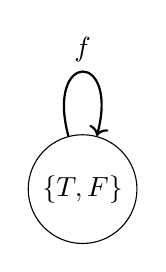
\begin{tikzpicture}
    % Define the node
    \node[circle, draw] (A) at (0,0) {$\{T,F\}$};
    
    % Draw self loop
    \draw[->, thick] (A) to[loop above] node[above] {$f$} (A);

\end{tikzpicture}
\end{center}

The above picture tells is that there \emph{is} a morphism called $f$, 
but it does not tell us anything about the \emph{content} of $f$. In particular, 
it is useful to know how $f$ maps elements of its domain to its codomain. 
To see this, we can draw the \textbf{internal picture} of this category
that visualizes the computational content of its morphisms:\footnote{Not 
all categories will have nice internal pictures, and different kinds of category 
will have their own visual language for describing their morphisms.}

\begin{center}
 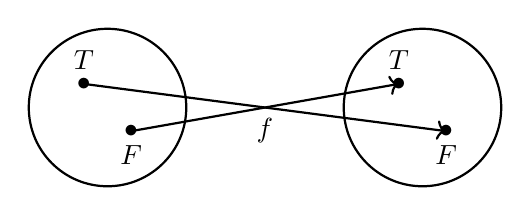
\begin{tikzpicture}
  % First circle with T and F dots
  \draw[thick] (0,0) circle (1);
  \node at (-0.3,0.3) {$\bullet$};
  \node at (-0.3,0.6) {$T$};
  \node at (0.3,-0.3) {$\bullet$};
  \node at (0.3,-0.6) {$F$};
  
  % Second circle with T and F dots
  \draw[thick] (4,0) circle (1);
  \node (T2) at (3.7,0.3) {$\bullet$};
  \node at (3.7,0.6) {$T$};
  \node (F2) at (4.3,-0.3) {$\bullet$};
  \node at (4.3,-0.6) {$F$};
  
    % Arrow from T on the left to F on the right
    \draw[->, thick] (-0.3,0.3) -- (4.3,-0.3);
    
    % Arrow from F on the left to T on the right
    \draw[->, thick] (0.3,-0.3) -- (3.7,0.3) node[midway, below] {$f$};
\end{tikzpicture}
\end{center}

Do not confuse the internal picture of a category with its picture: the internal 
picture ``peers inside objects'', and will not generalize to all kinds of categories.
This internal picture visualizes how the map $f$ behaves. A crucial 
piece information that this internal picture conveys is when two morphisms 
in \(\FinSet\) are equal: it is when they are \emph{extensionally equal}.

\todo: internal picture of \(\mathsf{not} \circ \mathsf{not} = \mathsf{id}\)


\section{Gaining intuition for categories}

The definition of category is highly abstract---and necessarily so, in order to be general enough
to accommodate all of the metalanguages just mentioned.
Next time, we will see how this level of abstraction allows for
clean axiomatizations of the various kinds of ``features'' that a metalanguage may support,
in the form of so-called ``universal constructions.''
This is what gives category theory its unifying power.

As preparation, we will first need to become quite comfortable working
with categories in the abstract. To do this, it is key to
have in mind a few representative examples of categories
to draw intuition from.

\subsection{Categories as graphs}

The first perspective on categories, which is perhaps most
comfortable to computer scientists, is that they are ``directed multigraphs with extra structure.''
Objects are vertices and morphisms are edges.
On top of this basic graph structure, categories come with a
composition operation that pastes two incident edges together to form a third,
and identity morphisms \(\mathsf{id}_A\) that form self-loops centered at each vertex \(A\).
The category laws then say that pasting of edges is an associative operation,
and that pasting with an identity morphism does nothing.
This provides nice visual intuition, and a large stock of example categories.
In fact,
\begin{construction}
  Every directed multigraph can be turned into a category.
\end{construction}
\begin{proof}
  Let \(G\) be a directed multigraph,
  encoded as a tuple \((V,E,\mathsf{src},\mathsf{trg})\)
  where \(V\) is the set of vertices, \(E\) is the set of edges,
  and \(\mathsf{src},\mathsf{trg}\) are functions \(E\to V\)
  that send each edge to its source and target vertices respectively.
  The graph \(G\) can be used to define a category
  \[
  \mathsf{paths}(G) = (O,M,\dom,\cod,\circ,\idt)
  \]
  where
  \begin{itemize}
  \item \(O = V\)
  \item \(M\) is the set of paths in \(G\),
    which are tuples \((v_s,[e_1,\dots,e_n],v_t)\)
    where \(v_s,v_t\) are vertices and \(e_1,\dots,e_n\) is a list of edges satisfying
    \(\mathsf{src}(e_1) = v_s\) and \(\mathsf{trg}(e_n) = v_t\)
    and \(\mathsf{trg}(e_i) = \mathsf{src}(e_{i+1})\)
    for all \(1\le i < n\).
  \item \(\dom : M \to O\) is the function \(\dom(v_s,[e_1,\dots,e_n],v_t) = v_s\)
  \item \(\cod : M \to O\) is the function \(\cod(v_s,[e_1,\dots,e_n],v_t) = v_t\)
  \item \(\circ\) concatenates paths:
    \((v_t,[f_1,\dots,f_n],v_u)\circ(v_s,[e_1,\dots,e_m],v_t) = (v_s,[e_1,\dots,e_m,f_1,\dots,f_n],v_u)\).
    Note that this is well-defined because the two paths \(\vec f\) and \(\vec e\) line up tip-to-tail.
    Note also that \(\vec e\) comes before \(\vec f\) in the concatenated path, due to the reversal of order
    of arguments to \(\circ\).
  \item \(\idt_v\) is the empty path \((v,[],v)\) starting and ending at \(v\).
  \end{itemize}
  The category laws are satisfied because concatenation of paths is associative and concatenating a path with the
  empty path does nothing.
\end{proof}
\begin{note}
  It is essential that morphisms are \emph{paths} in this construction, and not edges!
  Otherwise, it would be unclear how to define composition and identity.
\end{note}

\subsection{A Difference Between Categories and Directed Multigraphs}

A key difference between categories and graphs is that
two morphisms in a category that come from
different ``paths'' may nonetheless be equal.
For example, the following two ``paths'' through \(\FinSet\)
are actually the same, because negating a Boolean twice is the same as doing nothing:
\[% https://tikzcd.yichuanshen.de/#N4Igdg9gJgpgziAXAbVABwnAlgFyxMJZABgBpiBdUkANwEMAbAVxiRAB13gAVUgMU4BfEINLpMufIRQAmclVqMWbTj35CRYkBmx4CRAIykDC+s1aIOXXgPbDBCmFADm8IqABmAJwgBbJGQgOBBIRormKuy+dDgAFnAewJA49lrefqHUwUhy4cqWnNFxCUkQKZqePv6IgdmIuWb5VlhQOAD6wKo2QsLUDHQARjAMAAoSetIgXljOsTgiFIJAA
\begin{tikzcd}
{\{T,F\}} \arrow[rr, "\mathsf{not}"] \arrow[rd, "{\idt_{\{T,F\}}}"'] &           & {\{T,F\}} \arrow[ld, "\mathsf{not}"] \\
                                                                     & {\{T,F\}} &
\end{tikzcd}\]
This relationship between the paths \(\mathsf{not}\circ \mathsf{not}\) and \(\idt_{\{T,F\}}\)
is often conveyed by saying that the triangle above is ``filled in'', or ``commutes''.
The intuition being that one can then ``continuously deform''
\(\mathsf{not}\circ\mathsf{not}\) into \(\idt_{\{T,F\}}\),
by ``dragging'' it through the filled in triangle.

This idea is a handy visual tool for organizing categorical information
and for conducting proofs.

\subsection{Categories as orders}

A special case of a multigraph is a graph, where there is \emph{at most one} arrow between any given pair of vertices.
This leads us to the second class of important examples of a category:
\begin{definition}[preorder]
  \sloppy
  A preorder is a pair \((X,\preceq)\)
  where \(X\) is a set and \(\preceq\)
  is a binary relation on \(X\)
  that is reflexive (\(x\preceq x\) for all \(x\) in \(X\))
  and transitive (if \(x \preceq y\) and \(y\preceq z\) then \(x \preceq z\)).
\end{definition}
Preorders are often fruitfully drawn as \emph{Hasse diagrams}.
%% An object is like an element of a preorder
%% and a morphism \(x\to y\) is like a ``proof'' that \(x\le y\).
A simple example is the set \(\N\) of natural numbers,
ordered by \(m\preceq n\) if \(m\) is less than or equal to \(n\).
We can draw this preorder as follows:
\[
% https://tikzcd.yichuanshen.de/#N4Igdg9gJgpgziAXAbVABwnAlgFyxMJZABgBoBmAXVJADcBDAGwFcYkRiQBfU9TXfIRRkATNTpNW7AIzdeIDNjwEiZaeIYs2iECLl8lg1aWIbJ2kAB1LtKBBwIu4mFADm8IqABmAJwgBbJHIaHAgkERoACxh6KHZIMDYebz9AxAiQUKRpKJi4nQSk+V8A7JCwxDIQaNj4giTKLiA
\begin{tikzcd}
\vdots \arrow[d, no head] \\
2 \arrow[d, no head]      \\
1 \arrow[d, no head]      \\
0
\end{tikzcd}\]
Hasse diagrams are read bottom-up, with the least elements 
on the bottom and the greatest elements on the top. 
An undirected edge is drawn between elements with no elements 
between them (this is why we have no edge from 0 to 2 in the above figure).
A more visually interesting preorder on \(\N\)
is to define \(m \preceq n\) if \(m\) is a \emph{divisor} of \(n\).
This preorder looks less like a straight line and more like a lattice:
\[
% https://tikzcd.yichuanshen.de/#N4Igdg9gJgpgziAXAbVABwnAlgFyxMJZARgBoBmAXVJADcBDAGwFcYkRiQBfU9TXfIRQAGUgCZqdJq3ZjuvEBmx4CRMhJoMWbRCHLy+ywUTHjJWmboCsBxfxVDko4uek6QANltKBqlGRdNN3ZiYW97YxRTQKltEJseQ19HUWFXON0AHUzaKAgcBES7Iz9kUzSgjJBs3PzChR8HNVIK2MtqnLyC7kkYKABzeCJQADMAJwgAWyQyEBwIJFEQAAsYeih2SDA2IvGppFM5hcQl1fXNgh2FPenEchp5xZozjd0tq9GJ248H48OXi7bWw3JA-I5Ie4rNavcCXYFfJBWX4zZ7QwEfEAgxBI8F3VHnN5w3YIxAAFmRiH+aMJQOJ+zJFNmAJpGKx5NxAHZ8TD3vD6WDHogABzc9F8244wUATlFLJ6XCAA
\begin{tikzcd}
\vdots                                                      & \vdots                                                        & \vdots                                                       \\
6 \arrow[rd, no head] \arrow[d, no head] \arrow[u, no head] & 10 \arrow[ld, no head] \arrow[rd, no head] \arrow[u, no head] & 15 \arrow[ld, no head] \arrow[d, no head] \arrow[u, no head] \\
2 \arrow[rd, no head]                                       & 3 \arrow[d, no head]                                          & 5 \arrow[ld, no head]                                        \\
                                                            & 1                                                             &
\end{tikzcd}
\]
Preorders don't have to be discrete either: the real numbers \(\R\),
for instance, form a preorder with \(x \preceq y\) if \(x\) is less than or equal to \(y\). This is a little harder to draw.

A preorder that arises frequently in PL is the preorder of
\emph{run-time environments}.
It is common to model these environments
as partial functions \(\rho : \mathsf{Var} \rightharpoonup \mathsf{Val}\),
assigning to each program variable \(x \in \mathsf{Var}\)
a concrete value \(\rho(x)\).
These substitutions form a preorder, with \(\rho \preceq \rho'\)
if \(\rho\) is a subset of \(\rho'\), in the sense that all the 
variables in $\rho$ are in $\rho'$ and mapped to the same values.
%% \item Heaps under disjoint union: let \(\mathsf{Heap}\) be the category
%%   whose objects are substitutions \(\gamma\),
%%   i.e., partial functions \(\mathsf{Loc} \rightharpoonup \Z\),
%%   and whose morphisms from \(h\) to \(h'\)
%%   are heaps \(h_{\mathsf{diff}}\) such that \(h \uplus h_{\mathsf{diff}} = h\).

Preorders forms a category:
\begin{construction} \label{prop:every-preorder-is-a-category}
  Every preorder can be turned into a category.
  \label{eq:const-preorder}
\end{construction}
\begin{proof}
  For any preorder \((X,\preceq)\), there is a category
  \[
    \mathsf{order}(X,\preceq) = (O,M,\dom,\cod,\circ,\idt)
  \]
  where
  \begin{itemize}
    \item \(O = X\).
    \item \(M = (\preceq)\) (recall that a binary relation like \(\preceq\)
      can be thought of as a set of pairs, with \((x,y) \in (\preceq)\)
      if and only if \(x\preceq y\)).
    \item \(\dom\) is the function \(\dom(x,y) = x\).
    \item \(\cod\) is the function \(\cod(x,y) = y\).
    \item \(\circ\) is the function defined by \((y,z)\circ(x,y) = (x,z)\).
      Note that we may assume that the two arguments to \(\circ\)
      share a component \(y\) in this definition because of the assumption
      that \((y,z)\) and \((x,y)\) are composable.
      Note also that the composite \((x,z)\) is indeed well-defined
      this is well defined by the transitivity of \(\preceq\).
    \item \(\idt_x\) is the pair \((x,x)\), which forms a valid morphpism
      by reflexivity of \(\preceq\).
  \end{itemize}
  The category laws are satisfied automatically,
  as there can only be at most one morphism between any two objects.\footnote{Pause: 
  why is this the case?}
\end{proof}
\noindent
The intuitive import of Proposition~\ref{prop:every-preorder-is-a-category}
is that every category can be thought of as a kind of preorder,\footnote{\emph{Reminder}: not all 
categories directly correspond to some preorder construction, since there can be multiple 
morphisms between objects in a general category. A category with at most 1 morphism between 
any 2 objects is called a \emph{thin category}, and it does correspond to some preorder.}
where the existence of a morphism \(A\xrightarrow{f} B\)
expresses that \(A\) is in some sense ``less than or equal to'' \(B\).
Thinking of categories in this way leads to interesting questions like:
\begin{itemize}
\item
  Does a category have a ``smallest'' or ``largest'' object?
  For instance, the smallest runtime environment is the empty environment $\emptyset$
  with no variables in it.
\item Does a category have ``ascending sequences''?
  For example, 
  \begin{align}
   \emptyset \subseteq \{x\mapsto A\} \subseteq \{x\mapsto A, y\mapsto B\} \subseteq \dots 
   \label{eq:env-seq}
  \end{align}
  is an ascending sequence in the preorder of runtime environments.
\item  Does a category have ``limit'' objects, like suprema or infima?  For
  instance, you probably know from calculus that there limits in \(\R\): for
  example, the sequence $\frac{1}{2}, \frac{1}{4}, \frac{1}{8},
  \frac{1}{16}\cdots$ approaches 0 in the limit.  A very interesting question is:
  which categories ``have limits'', in the sense that such sequences always
  converge to some object in the category?

  An example of a situation where there is no limit is the sequence in
  \cref{eq:env-seq}.  The set of environments grows and grows, and since there
  is no notion of a ``greatest environment'', there is no limit to this
  sequence.
\item
  Given two categories, is there a notion of ``monotone map'' between them?
\end{itemize}

Each of the above observations is foreshadowing a notion of a ``universal construction''
in a category, which we will explore in the following lectures.

\subsection{Categories as algebras}

Whereas preorders are like multigraphs where there is at most one \emph{edge}
between any two vertices,
the opposite extreme is a multigraph with exactly one \emph{vertex},
so that all edges are self-loops:
% https://q.uiver.app/#q=WzAsMSxbMCwwLCJcXGJ1bGxldCJdLFswLDBdLFswLDAsIiIsMCx7InJhZGl1cyI6MX1dLFswLDAsIiIsMCx7InJhZGl1cyI6NX1dXQ==
\begin{equation}
\begin{aligned}
\begin{tikzcd}
	\star
	\arrow[from=1-1, to=1-1, loop, in=55, out=125, distance=10mm]
	\arrow[from=1-1, to=1-1, loop, in=60, out=120, distance=5mm]
	\arrow[from=1-1, to=1-1, loop, in=50, out=130, distance=15mm]
\end{tikzcd}
\end{aligned}
\end{equation}
Categories of this shape form our final class of important example:
a special kind of algebraic structure called a \emph{monoid}.
\begin{definition}[monoid]
  A monoid is a tuple \((X,\bullet,e)\)
  where \(\bullet\) is a binary operation on \(X\)
  (a function \(X \times X \to X\))
  that is associative (\(x\bullet (y\bullet z) = (x\bullet y) \bullet z\))
  and has \(e\) as a unit (\(x\bullet e = x\) and \(e\bullet x = x\)).
\end{definition}
A simple example of a monoid is \((\N,+,0)\),
the monoid of natural numbers under addition.
This forms a monoid because addition of natural numbers is associative
and has zero as a unit.

An example that is closer to PL
comes from the semantics of imperative programs.
It is common to interpret an imperative program
as a function \(S \to S\), where \(S\) is a set of
memory states.
For example, the program
\[
  x := x + 1;
\]
can be interpreted
as a function that sends a memory state \(s\)
to a new memory state \(s'\) in which
the value of \(x\) has been incremented by \(1\).
The functions \(S \to S\) form a monoid
\((S\to S,\bullet,\mathsf{id})\),
where the monoid operation is given by \(f \bullet g = g \circ f\)
(note the reversal!),
corresponding to the sequencing of the programs \(f\) and \(g\),
and the identity element is the identity function on \(S\),
corresponding to the empty program that does nothing.

Algebraic identities capture program rewrites for this imperative language.
For example, if \(f\) is the interpretation of \(x := 0\)
and \(g\) is the interpretation of \(y := 1\),
and \(x\) and \(y\) are distinct program variables,
then the program equation
\begin{equation}
  \left(\begin{aligned}
    &x := 0 \\
    &y := 1
  \end{aligned}\right)
  \equiv
  \left(\begin{aligned}
    &y := 1 \\
    &x := 0
  \end{aligned}\right)
\end{equation}
can be expressed as the algebraic identity \(g \circ f = f \circ g\).

\begin{construction} \label{prop:every-monoid-is-a-category}
  Every monoid can be turned into a category.
\end{construction}
\begin{proof}
  For any monoid \((X,\bullet,e)\) there is a category
  \[
    \mathsf{mon}(X,\bullet,e) = (O,M,\dom,\cod,\circ,\idt)
  \]
  where
  \begin{itemize}
  \item \(O = \{\star\}\), a singleton set with a single dedicated element \(\star\).
    \marginnote{Technically set theory does not contain stars in it.
    But this is no matter.
    The symbol \(\star\) can be interpreted as any object of
    your choice---all that matters
    is that \(O\) is a singleton set.
    For instance, one could set \(\star =
    \varnothing\).
    }
  \item \(M = X\)
  \item \(\dom(M) = \star\)
  \item \(\cod(M) = \star\)
  \item Composition is defined by \(x \circ y = x \bullet y\)
  \item \(\idt_\star = e\)
  \end{itemize}
  The category laws follow from the associativity of \((\bullet)\)
  and that it has \(e\) as a unit.
\end{proof}
\begin{note}
  It is very important that the set of objects \(O\) is a singleton set \(\{\star\}\).
  A natural thought one might have is that the set of objects should be the set \(X\) of elements of the monoid.
  But this in fact does not work: what would be the morphisms?

  There is actually a good reason why the set of objects is the seemingly-arbitrary singleton set \(\{\star\}\) in this construction.
  It comes from the fact that a monoid is what is called a \emph{single-sorted} algebraic structure; hence \(\{\star\}\)
  is a set with a single element.
\end{note}
The intuitive import of
Proposition~\ref{prop:every-monoid-is-a-category} is that
every category can be thought of as a kind of algebraic structure,
where composition is like ``multiplication''
and identity morphisms are like ``multiplicative units''.

The algebraic perspective leads to questions like:
given an equation between morphisms containing some unknowns,
are there zero, one, or infinitely many solutions?
When can I ``cancel'' a morphism from both sides of an equation (e.g., from \(fg = fh\) deduce \(g=h\),
or from \(fh = gh\) deduce \(f=g\))?
When does a morphism have an ``inverse''?
When can a morphism \(f\) be ``factored'' into two pieces, \(f = gh\)?


\section{Putting intuitions to the test}

We conclude this section by illustrating each of the three perspectives
on categories on the following
\textbf{categorification}\footnote{The idea of ``categorification'' is to 
cast a notion one is familiar with -- like ``subset inclusion'' into 
the language of objects and morphisms. This is a very important idea 
in category theory because it allows one to take familiar concepts 
and apply them to unfamiliar categories.} of
a basic concept from set theory: subset inclusion.
\begin{proposition} \label{prop:subset-leq-iff-triangle}
Suppose \(U\) and \(V\) are subsets of a finite set \(X\).
Then \(U \subseteq V\) if and only if
there exists a dashed \(\FinSet\)-morphism \(f\)
such that \(f \circ v = u\),
where \(u\) and \(v\) are the \(\FinSet\)-morphisms
corresponding to the inclusion functions\footnote{A function $f : X \to Y$ 
is an \emph{inclusion function} (also called an ``injective map'') if 
each element of $X$ is mapped to a unique element in $Y$. 
All inclusion functions have a ``left inverse'': 
there exists a function $g$ such that $g \circ f = \mathsf{id}_X$.
Inclusion maps are rendered using tailed arrows.} \(U \to X\) and \(V \to X\)
respectively:
\begin{equation}
  % https://tikzcd.yichuanshen.de/#N4Igdg9gJgpgziAXAbVABwnAlgFyxMJZABgBpiBdUkANwEMAbAVxiRAFUQBfU9TXfIRQAmclVqMWbAGrdeIDNjwEiARlKrx9Zq0QgAGt3EwoAc3hFQAMwBOEALZIyIHBCSiXdLAzY4vP6m0pPSYQagY6ACMYBgAFfmUhEBssUwALHDlrO0dEdRc3RA8-b19-MIkdNhoskFsHJ2pXJHySnz1IMFZwrC62KDo4NJMKoN06oy4gA
\begin{tikzcd}
U \arrow[rd, "u"', tail] \arrow[rr, "f", dashed] &   & V \arrow[ld, "v", tail] \\
                                                 & X &
\end{tikzcd}
\end{equation}
\end{proposition}
You will prove Proposition~\ref{prop:subset-leq-iff-triangle} in the homework.
As preparation,
let's appreciate what it is saying: a basic set theoretic
property \(U\subseteq V\) about finite subsets
can be recast in terms of a purely category-theoretic property
about \(\FinSet\).
This categorification takes roughly two steps.
The first step is to express the subsets \(U\) and \(V\)
as morphisms \(u\) and \(v\).
The second step is to express \(U\subseteq V\)
as a property of the morphisms \(u\) and \(v\).
Let's try to get some intuition for what this property is saying
from each of the perspectives we've developed so far.
\begin{itemize}
\item Graphically, it says that the morphisms \(u\) and \(v\)
  fit into a triangle with \(f\) that is ``filled in''.
\item Order-theoretically, it says that the morphism \(u\) is somehow
  ``less than or equal to'' \(v\), by virtue of there being a dashed morphism
  \(f\) witnessing this order relationship.

  We can make this formal as follows.
  For any finite set \(X\), one can construct a category \(\mathsf{Sub}(X)\).
  The objects of this category are tuples \((U,u)\) where \(U\) is a subset of \(X\)
  and \(u\) is the function \(U \to X\) defined by \(u(x) = x\);
  i.e., \(u\) is the canonical inclusion function of \(U\) into \(X\).
  The morphisms of this category are, roughly speaking,
  pictures of the following shape:
  \[
  % https://tikzcd.yichuanshen.de/#N4Igdg9gJgpgziAXAbVABwnAlgFyxMJZABgBpiBdUkANwEMAbAVxiRAFUQBfU9TXfIRQBGUsKq1GLNgA1uvEBmx4CRAEzkJ9Zq0QgAatwkwoAc3hFQAMwBOEALZIyIHBCSjJOtkxDUGdACMYBgAFfhUhEBssUwALHHlrO0dEDRc3RA9taT0aRJBbBydqVyQ07N0Coy4gA
\begin{tikzcd}
U \arrow[rd, "u"'] \arrow[rr, "f"] &   & V \arrow[ld, "v"] \\
                                   & X &
\end{tikzcd}
  \]
  Formally, a morphism is a tuple \((U,u,f,V,v)\)
  where \(U\) and \(V\) are subsets of \(X\),
  \(u : U \to X\) and \(v : V \to X\) are the canonical inclusions,
  and \(f\) is a function \(U \to V\)
  such that \(v \circ f = u\).
  Each morphism \((U,u,f,V,v)\) has domain \((U,u)\)
  and codomain \((V,v)\).

  Now Proposition~\ref{prop:subset-leq-iff-triangle}
  says that \(U\subseteq V\) if and only if there is a morphism from \((U,u)\)
  to \((V,v)\) in the category \(\mathsf{Sub}(X)\),
  witnessing the fact that \((U,u)\) is ``less than or equal to'' \((V,v)\).

\item Algebraically, it says that the equation \(u = f \circ v\)
  has a solution in the unknown \(f\).
\end{itemize}
Let's see each of these in action on the following proof.
\begin{proposition}
  If \(U\subseteq V\) and \(V \subseteq W\) then \(U\subseteq W\).
\end{proposition}
Each perspective lends itself to a different proof strategy.
\begin{itemize}
\item Graphically, you paste two filled in triangles to get a bigger filled in triangle.
\item Order-theoretically, you use the fact that \(\mathsf{Sub}(X)\), as a category,
  has composition.
\item Algebraically, you use that \(u = vf = wvg\) provides a solution to \(u = wh\).
\end{itemize}

%% \item Refinement corresponds to solvability of an equation that looks like a square.
%%   Suppose you have a subset \(U\) of a finite set \(X\),
%%   a subset \(V\) of a finite set \(Y\),
%%   and a function \(f : X \to Y\).
%%   Let \(u : U \rightarrowtail X\) and \(v : V \rightarrowtail Y\) be the relevant inclusions.

%%   Suppose \(f\) satisfies the property that,
%%   for all \(x \in U\), it holds that \(f(x) \in V\).
%%   This can be expressed as saying that the equation
%%   \(fu = vg\) is \emph{solvable} in the unknown \(g\).
%%   Diagramatically:
%%   \[
%%   % https://tikzcd.yichuanshen.de/#N4Igdg9gJgpgziAXAbVABwnAlgFyxMJZABgBpiBdUkANwEMAbAVxiRAFUQBfU9TXfIRQBGclVqMWbAGrdeIDNjwEiZYePrNWiEAA05fJYKKj11TVJ0BNbuJhQA5vCKgAZgCcIAWyRkQOCCQAJmocOiwGNjCIkHNJbRAmWJAGOgAjGAYABX5lIRB3LAcACxwDEA9vJFF-QMQAZlDwyJ1oyLitNhpyyp9EPwDqjssQBx7PPpDapEaJTp1XZNSM7NzjHUKSsq4KLiA
%% \begin{tikzcd}
%% U \arrow[d, "u"', tail] \arrow[r, "g"] & V \arrow[d, "v", tail] \\
%% X \arrow[r, "f"']                      & Y
%% \end{tikzcd}
%%   \]
%%   This situation actually comes up quite a lot in PL,
%%   as we will see when we discuss logical relations.

%%   (By the way, the solution \(g\), if it exists, must be the \emph{only} solution to this equation,
%%   as if one finds \(g\) and \(g'\) such that \(fu = vg\) and \(fu = vg'\), then \(vg=fu=vg'\),
%%   and left-cancellativity of \(v\) implies \(g = g'\).)

\subsection{Some fun exercises}

\begin{itemize}
\item Explicitly write down the monoid \((\N,+,0)\) as a category.
\item Solve the equation \(c \circ (x := x + 1) = (x := x + 2)\) for \(c\).
  Can you find any other solutions?
\item Try to come up with an English description of what it means for an Imp command to be ``left'' or ``right'' cancellable
\item Prove Proposition~\ref{prop:subset-leq-iff-triangle}.
\item Show that the functions \(u,v\) in Proposition~\ref{prop:subset-leq-iff-triangle}
  are left-cancellable as morphisms of \(\FinSet\).
\end{itemize}

\chapter{Universal Constructions I}
We've been hinting at the utility of knowing that categories that have certain
special objects in them. For example, if we want to give a category that lets us
validate equations of programming languages, that category will need to be able 
to represent the many features that programs might have: products, sums, 
functions, etc. Here we will introduce the essential idea of a \textbf{universal 
construction} that characterizes when categories contain these special objects.

\section{Terminal objects \& the unit type}
Recall that when designing categorical semantics for programming languages we
associate types and typing contexts with objects in the category and terms with
morphisms. Concretely, if we have a well-typed term $\Gamma \vdash e : A$,
its interpretation $\dbracket{\Gamma \vdash e : A}$ is a morphism
$\dbracket{\Gamma} \xrightarrow{\dbracket{e}} \dbracket{A}$.
Previously, we showed how \(\FinSet\) can be used to give an interpretation 
to \ref{lang:calc} programs by associating types like the unit type $\plUnit$
with special sets, like a set containing only a single element $\{\star\}$.
But, what if we want to see if categories other than $\FinSet$ can give give a 
reasonable interpretation for $\plUnit$?

To proceed, let's pick a particular object $\dbracket{\plUnit}$ 
in a category $\calC$ and explore what properties it needs to have in order 
to be ``$\plUnit$-like'':
\begin{itemize}
  \item \textbf{Fact 1, Introduction rules}: It must be possible in any typing context to
  produce a value of type $\plUnit$.  This tells us that for any context
  $\Gamma$, there must exist a $\calC$-morphism
  $\dbracket{\Gamma} \to \dbracket{\plUnit}$.
  For example, it must 
  be the case that 
  $\dbracket{\Gamma} \xrightarrow{\dbracket{\plunit}} \dbracket{\plUnit}$.

  \item \textbf{Fact 2, Equational laws}: Since \ref{lang:calc} has no effects, 
  it is the case that if $\Gamma \vdash e : \plUnit$, then it is indistinguishable 
  from the term $\plunit$. This is called \textbf{eta equality}, and we write
  this as $e \equiv \plunit$.\footnote{The symbol ``$\equiv$'' means ``is
  equationally equal to''.} Eta equality is an equational law that characterizes
  how a $\plUnit$ term must behave. Now for an insight: \emph{these equational
  laws are translated into morphism equalities}. It must be that, for any
  morphism $\dbracket{\Gamma} \xrightarrow{\dbracket{e}} \dbracket{\plUnit}$, it
  is the case that $\dbracket{e} = \dbracket{\plunit}$.  In other words, the
  morphism $\dbracket{\Gamma} \xrightarrow{\dbracket{\plunit}} \plUnit$ must be
  unique.
\end{itemize}

These two properties can be packaged up into a nice concise definition:

\begin{definition}[Terminal object]  \label{def:terminal-object}
  Let $T$ be an object in a category $\calC$. 
  An object $T$ in $\calC$ is called a terminal object
  if
  \begin{itemize}
  \item
    for every object \(\Gamma\) in \(\calC\)
    there is a morphism \(\Gamma \xrightarrow{\angled{}} T\);
  \item
    for every morphism \(\Gamma \xrightarrow{f} T\)
    it holds that \(f = \angled{}\).
  \end{itemize}
\end{definition}

Let's pause to remark on the three categorical interpretations 
of terminal objects $T$:
\begin{itemize}
  \item Graphically, an object is terminal if (1) there is an arrow from 
  every other object to it, and (2) it ``thins all parallel
  arrows'', meaning that if we have a situation like the following for 
  and morphisms $X \xrightarrow{f} T, X \xrightarrow{g} T$:
  \begin{align*}
    % https://tikzcd.yichuanshen.de/#N4Igdg9gJgpgziAXAbVABwnAlgFyxMJZABgBpiBdUkANwEMAbAVxiRABUQBfU9TXfIRRkAjFVqMWbABrdxMKAHN4RUADMAThAC2SEdRwQkZEACMYYKEgC0AZhMM65hgAV+eAmw1ZFACxwg1PTMrIggity8IJo6egZGiCbmlkj21I7ObtgeQiAMMGoBQZKh0XJcQA
\begin{tikzcd}
  T                                                       \\
  X \arrow[u, "g"', bend right] \arrow[u, "f", bend left]
  \end{tikzcd},
  \end{align*}
  then we know that $f = g$.
  In other words, there is a unique morphism \(\Gamma \to T\) for every \(\Gamma\):
  \begin{center}
% https://tikzcd.yichuanshen.de/#N4Igdg9gJgpgziAXAbVABwnAlgFyxMJZABgBpiBdUkANwEMAbAVxiRAEEQBfU9TXfIRQBGclVqMWbACrdxMKAHN4RUADMAThAC2SMiBwQkokAyxhWiEHAhmoIagzoAjGAwAK-PATYMYanAcJZksQAB0wmAAPLDgcOABCOS4gA
\begin{tikzcd}
  A \arrow[r, "\exists!"] & T
  \end{tikzcd}
\end{center}
  \item The order-theoretic perspective is that the terminal object 
  is the ``greatest object'' in the category.
  \item The algebraic perspective
    says that, for every object \(\Gamma\),
    the equation \(f = f\) has a unique solution
    in the unknown \( \Gamma \xrightarrow{f} T\).
\end{itemize}

We say a category \textbf{has terminal objects} if there is an object in the
category that is a terminal object. This is our first example of a 
\textbf{universal construction}, which are special objects in categories 
characterized by their morphisms into them. We will see how universal 
constructions can be used to give interpretations to all the type 
formers we have seen so far. But, we can already see their utility: 
whether or not a particular category admits certain universal constructions
will immediately inform us of that category's suitability for modeling 
certain language properties.

\subsection{$\FinSet$ has terminal objects, isomorphisms}
We saw in previous lectures that we could use the singleton set 
$\{\star\}$ to give an interpretation to $\plUnit$ in $\FinSet$.
We can easily prove that $\{\star\}$ is a terminal object:
\begin{theorem}
  The singleton set $\{\star\}$ is terminal in $\FinSet$.
\end{theorem}
\begin{proof}
  \begin{itemize}
    \item Existence: The map $\_ \mapsto \{\star\}$ has the required type.
    \item Uniqueness: Suppose we have two morphisms $A \xrightarrow{f} \{\star\}$ and
    $A \xrightarrow{g} \{\star\}$. 
    Then by function extensionality we immediately have that $f = g$ 
    as set-functions, and so they are equal as $\FinSet$ morphisms.
  \end{itemize}
\end{proof}

Now you can observe the above proof and see that it immediately 
works for \emph{any} choice of singleton set: does this mean that $\FinSet$
has \emph{many terminal objects?} Yes, and no. \emph{Yes}, in the sense 
that there are indeed many valid choices of terminal object; but \emph{no}, 
in the sense that the choice itself does not (\emph{should} not!) actually 
matter. We capture this by the notion of isomorphism:

\begin{definition}[Isomorphism of objects]
  \sloppy
  Two objects $A$ and $B$ in a category $\calC$ are isomorphic if 
  there exist morphisms $A \xrightarrow{f} B$ and $B \xrightarrow{g} A$
  such that (1) $g \circ f = \id_A$ and (2) $f \circ g = \id_B$.
\end{definition}

We can immediately see that any two singleton sets in $\FinSet$ are isomorphic:
this proof is straightforward. What might be surprising is that this 
fact is true for all terminal objects:

\begin{theorem} \label{thm:terminal-object-unique}
  Terminal objects are unique up to isomorphism.
\end{theorem}
\begin{proof}
  Let $X$ and $Y$ be terminal objects in some category $\calC$. 
  Then there exists a pair of unique morphisms between them:

  \begin{center}
 % https://tikzcd.yichuanshen.de/#N4Igdg9gJgpgziAXAbVABwnAlgFyxMJZABgBpiBdUkANwEMAbAVxiRAA0QBfU9TXfIRQBGclVqMWbAJrdxMKAHN4RUADMAThAC2SMiBwQkokACMYYKEgDM++s1aIQAQjXdeITTuPVDe6uaWNnaSji6KclxAA
\begin{tikzcd}
  X \arrow[r, "!f", bend left] & Y \arrow[l, "!g", bend left]
  \end{tikzcd} 
\end{center}
By the fact that $X$ and $Y$ are terminal, they must also have unique identity
morphisms $\id_X$ and $\id_Y$. Then by the uniqueness of identity we have that $f \circ g = \id_X$ and $g \circ f = \id_Y$.
\end{proof}

This provides some evidence that the choice of terminal object does not matter.
  But are we done? Suppose we had two terminal objects \(T\) and \(T'\).
  By the above argument, we have that these two objects are isomorphic.
  But now another potential choice arises: what if there are multiple different
  \emph{isomorphisms} between \(T\) and \(T'\)?
  Then it could be that the choice to use \(T\) instead of \(T'\)
  may implicitly come with a choice of specific isomorphism as well.

  Luckily, terminal objects satisfy a stronger property
  which ensures that one's choice is terminal object is truly irrelevant.

\begin{proposition}
  Terminal objects are unique up to \emph{unique} isomorphism.
  That is, if \(T\) and \(T'\) are both terminal,
  then there is exactly one isomorphism
  \((f:T\to T',g:T'\to T)\)
  between \(T\) and \(T'\).
\end{proposition}
\begin{proof}
  Both \(f\) and \(g\), as constructed in the proof of
  \Cref{thm:terminal-object-unique},
  are the only possible morphisms \(T \to T'\) and \(T'\to T\)
  respectively. Thus they together form the only isomorphism
  between \(T\) and \(T'\).
\end{proof}

Later on, when we have the language for it, we will show that
all universal constructions are unique up to unique isomorphism
in this sense, and hence free of non-canonical choices.


% \subsection{Terminal objects for preorders}
% Universal constructions are one of the engines for analogy in category theory:
% very different-seeming concepts can be cast as instances of the same 
% universal construction, which can bring clarity to what each of those disparate 
% concepts means. When cast order-theoretically, the terminal object can 
% be thought of as ``the greatest object in a category.''
% % The first instance we will see of a universal construction is a \textbf{terminal 
% % object}, which can be thought of as ``the largest object in a category'' if one 
% % recalls the preorder intuition of morphisms. 

% An element of a preorder is the largest if it is greater than every other 
% element: i.e., there exists a morphism from every other element to it.
% This definition works for a general category: one could say an object is 
% largest if there exists a morphism from every other object into it.
% This characterization however doesn't take into account that there 
% can be more than 1 morphism between any two objects in a category: intuitively, 
% this means that one object can be greater than another in more than one way.

\section{Products}
Next we want to interpret product types $A \times B$. As before with the 
unit type, the typing rules for products forces the existence of certain morphisms,
and the equational theory of products forces equalities of certain morphisms.
The  introduction rule that describes how to create new products is:
\begin{mathpar}
\inferrule
    {\Gamma\vdash M : A
      \\
    \Gamma\vdash N : B
    }
    {\Gamma \vdash \plpair{M}{N} : A \pltimes B}~(\textsc{T-Pair})
\end{mathpar}
The elimination rules that break apart products are:
\begin{mathpar}
\inferrule
    {\Gamma\vdash M : A \pltimes B}
    {\Gamma \vdash \plfst{M} : A}~(\textsc{T-Fst})
\and
\inferrule
    {\Gamma\vdash M : A \pltimes B}
    {\Gamma \vdash \plsnd{M} : B}~(\textsc{T-Snd})
\end{mathpar}

These rules imply the existence of several morphisms that characterize 
what it means for for a special object $\dbracket{A \times B}$ to be a 
product. Reading off from the rules:
\begin{itemize}
  \item The \textsc{T-Pair} rules says that if there are 
  two morphisms $\dbracket{\Gamma} \mor{\dbracket{M}} \dbracket{A}$ and 
  $\dbracket{\Gamma} \mor{\dbracket{N}} \dbracket{B}$, 
  then there is a morphism $\dbracket{\Gamma} \mor{\dbracket{\langle M, N \rangle}} 
  \dbracket{A \times B}$.
  \item The \textsc{T-Fst} rule says that if there is a morphism 
  $\dbracket{\Gamma} \mor{\dbracket{M}} 
  \dbracket{A \times B}$, then there is a 
  morphism $\dbracket{\Gamma} \mor{\dbracket{\plfst{-}}} \dbracket{A}$.\footnote{Note:
  We are naming these morphisms \emph{suggestively}. The typing rules only enforce 
  the \emph{existence} of certain morphisms: they don't tell us anything about 
  how they behave.}
  \item The \textsc{T-Snd} rule says that if there is a morphism 
  $\dbracket{\Gamma} \mor{\dbracket{M}} 
  \dbracket{A \times B}$, then there is a 
  morphism $\dbracket{\Gamma} \mor{\dbracket{\plsnd{-}}} \dbracket{B}$.
\end{itemize}

We can package these morphisms up into the following diagram:

\begin{equation}
 % https://tikzcd.yichuanshen.de/#N4Igdg9gJgpgziAXAbVABwnAlgFyxMJZARgBoAGAXVJADcBDAGwFcYkQAdDgcXoFs+9EAF9S6TLnyEUZYtTpNW7AIIACLnj7xVAIRFiQGbHgJFypAEzyGLNohDL9441KIXL1xXZB7h8mFAA5vBEoABmAE4QfEjmIDgQSGQKtuxcjPRggYwwqgCypKoAclwRmdm5TiCR0Uk0CUjuIBkARjCMAAoSJtIgEViBABY4IDQ2SvZhcCOi4VExiMkNiADMNK3tXS6m9jlhI2Ne7HBgUFU1C3HLTW2nSAC0K3Hj3nnn87H1ias0t2erzyO9iKIkowiAA
\begin{tikzcd}[column sep = huge]
  & \dbracket{\Gamma} \arrow[d, "{\dbracket{\langle M, N\rangle }}"] \arrow[ldd, "\dbracket{M}" description, bend right] \arrow[rdd, "\dbracket{N}" description, bend left] &   \\
  & \dbracket{A \times B} \arrow[ld, "\dbracket{\plfst{-}}"' description] \arrow[rd, "\dbracket{\plsnd{-}}" description]                                                     &   \\
\dbracket{A} &                                                                                                     & \dbracket{B}
\end{tikzcd}
\label{cd:prod1}
\end{equation}

Next, the equational theory of products will assert certain equalities of
morphisms. We begin with the \emph{$\beta$-rules} that give the equational 
behavior of elimination after introduction:
% (elim after intros sometimes called \(\beta\) rules)
\begin{mathpar}
\inferrule
    {\Gamma\vdash M : A
      \\
    \Gamma\vdash N : B
    }
    {\Gamma \vdash \plfst{\plpair{M}{N}} \equiv M : A}~(\beta^{\pltimes}_1)
\and
\inferrule
    {\Gamma\vdash M : A
      \\
    \Gamma\vdash N : B
    }
    {\Gamma \vdash \plsnd{\plpair{M}{N}} \equiv N : B}~(\beta^{\pltimes}_2)
\end{mathpar}
Translating these equations into morphism equalities:
\begin{itemize}
  \item $\beta_1$ enforces that $\dbracket{M} = 
  \dbracket{\plfst{-}} \circ \dbracket{\langle M, N \rangle}$ 
  in (\ref{cd:prod1})
  \item $\beta_2$ enforces that $\dbracket{N} = 
  \dbracket{\plsnd{-}} \circ \dbracket{\langle M, N \rangle}$ 
  in (\ref{cd:prod1})
\end{itemize}

Hence, the $\beta$-rules together enforce that the diagram in \ref{cd:prod1} commutes.
Next, we consider the second part of the equational theory of products
that describes the behavior of introduction after elimination, sometimes called the \emph{\(\eta\)-rules}:
\begin{mathpar}
\inferrule
    {\Gamma\vdash M : A \pltimes B
    }
    {\Gamma \vdash M \equiv \plpair{\plfst{M}}{\plsnd{M}} : A \pltimes B}~(\eta^{\pltimes})
\end{mathpar}

This law says asserts the extensional equality of any two pair-formation
operations.  Translated into morphisms, it says that any morphism of the form
$\dbracket{\Gamma} \mor{\dbracket{M}} \dbracket{A \times B}$ is is equal to a
canonical morphism $\dbracket{\Gamma} \mor{\dbracket{\langle \plfst{M},
\plsnd{M} \rangle}} \dbracket{A \times B}$.  Put another way: there is a unique
morphism $\dbracket{\Gamma} \mor{} \dbracket{A \times B}$ amking the above diagram commute.

\subsection{Packaging up intuition into a definition}
Now, as in the case of terminal objects, we can give a more generic description of 
products that isn't so specific to the case of equational theories of programs:

\begin{definition}[Product] \label{def:product}
  Let \(A\) and \(B\) be two objects of a category \(\calC\).
  A \emph{product of \(A\) and \(B\)}
  is a tuple \((P,\pi_A,\pi_B)\)
  where
  \begin{itemize}
  \item \(P\) is an object of \(\calC\).
  \item \(\pi_A\) is a morphism from \(P\) to \(A\),
    called the \emph{projection onto \(A\)}.
  \item \(\pi_B\) is a morphism from \(P\) to \(B\),
    called the \emph{projection onto \(B\)}.
  \end{itemize}
  such that
  \begin{itemize}
  \item For any object \(\Gamma\) and any two morphisms \(f : \Gamma \to A\)
    and \(g : \Gamma \to B\),
    there exists a morphism \(\angled{f,g} : \Gamma \to P\)
    such that the following equations hold:
    \begin{align}
      \pi_A \circ \angled{f,g} = f \\
      \pi_B \circ \angled{f,g} = g
    \end{align}
  \item The following equation holds for any morphism \(h : \Gamma \to P\).
    \begin{align}
      h = \angled{\pi_A \circ h, \pi_B \circ h}
    \end{align}
  \end{itemize}
\end{definition}

\begin{proposition}
  Let \(A\) and \(B\) be finite sets.
  The tuple \((A \times B, \pi_A, \pi_B)\)
  is a product in \(\FinSet\),
  where \(\pi_A\) is the morphism \((A\times B,\pi_A, A)\)
  and \(\pi_B\) is the morphism \((A \times B,\pi_B,B)\).
\end{proposition}

\begin{proposition}
  Let \(A\) and \(B\) be two objects of a category \(\calC\).
  A tuple \((P,\pi_A,\pi_B)\) is a product of \(A\) and \(B\)
  if and only if the following \textbf{universal property}
  holds:
  for any object \(\Gamma\) and any two morphisms \(f : \Gamma \to A\)
  and \(g : \Gamma \to B\),
  there exists a unique morphism \(h : \Gamma \to P\)
  such that \(\pi_A \circ h = f\) and \(\pi_B \circ h = g\).
\end{proposition}
\begin{proof}
  Suppose \((P,\pi_A,\pi_B)\) is a product of \(A\) and \(B\).
  By definition of product, we have for any \(\Gamma\) and morphisms \(f : \Gamma \to A\)
  and \(g : \Gamma \to B\)
  that the morphism \(\angled{f,g} : \Gamma \to P\)
  satisfies \(\pi_A \circ \angled{f,g} = f\)
  and \(\pi_A \circ \angled{f,g} = g\).
  This morphism is the unique such, because
  if any morphism \(h : \Gamma \to P\)
  satisfies \(\pi_A \circ h = f\) and \(\pi_B \circ h = g\)
  then it must be that
  \begin{equation}
    h = \angled{\pi_A \circ h, \pi_B \circ h} = \angled{f,g}.
  \end{equation}
  Conversely, if \((P,\pi_A,\pi_B)\) is any tuple satisfying
  the above universal property,
  then one can define \(\angled{-,-}\)
  as the function that sends each pair of morphisms \(f : \Gamma \to A\)
  and \(g : \Gamma\to B\)
to the unique \(h\) such that \(\pi_A \circ h = f\) and \(\pi_A \circ h = g\).
\end{proof}

Algebraically, the universal property can be formulated as saying
  the following system of equations has exactly one solution
  in the unknown \(h : \Gamma \to P\).
  \begin{align}
    \pi_A \circ h = f \\
    \pi_B \circ h = g
  \end{align}
Diagramatically, it can be formulated as saying there exists a unique
dashed arrow that fills in all the triangles in the following picture.
\begin{equation}
% https://tikzcd.yichuanshen.de/#N4Igdg9gJgpgziAXAbVABwnAlgFyxMJZABgBoBGAXVJADcBDAGwFcYkQAdDgcXoFs+9EAF9S6TLnyEU5CtTpNW7AAoixIDNjwEiAJlLF5DFm0QgAgmvFape0rqOLTIAEIj5MKAHN4RUADMAJwg+JDIQHAgkfQUTdn8QGgAjGDAoJABmYlEA4NDEcMikWRBGLDBnKHo4AAtPRNilMxqrECCQsJoixAyaYyaQLwbGehTGZQltaRBArC8anAaUtKQAWiyctrzirqjEGP7nNGHRmHHJ2zNZ+cXN9vyS7t7G5wBHd2EgA
\begin{tikzcd}
                                                                                        &                                    & A \\
\Gamma \arrow[rru, "f", bend left] \arrow[r, "h", dashed] \arrow[rrd, "g"', bend right] & P \arrow[ru, "\pi_A"'] \arrow[rd, "\pi_B"] &   \\
                                                                                        &                                    & B
\end{tikzcd}
\end{equation}
Order-theoretically, a product of \(A\) and \(B\) is the ``greatest diagram'' of
the following shape, where the question marks are filled in with concrete objects and morphisms of \(\calC\):
\[
% https://tikzcd.yichuanshen.de/#N4Igdg9gJgpgziAXAbVABwnAlgFyxMJZARgBoAGAXVJADcBDAGwFcYkQB+EAX1PU1z5CKcqWLU6TVuwCCPPiAzY8BIgCYxEhizaIQAIR4SYUAObwioAGYAnCAFskokDghIykney41G9AEYwjAAKAirCIDZYpgAWOPLWdo6Izq5IGp7SelzclNxAA
\begin{tikzcd}
  & ? \arrow[ld, "?"'] \arrow[rd, "?"] &   \\
A &                                    & B
\end{tikzcd}
\]
We will make this perspective more precise in Section~\ref{sec:products-as-terminal-objects}.

Finally, as is the case with terminal objects, we say a category \textbf{has
products} if for any two objects $A$ and $B$ in a category there exists an 
object $A \times B$ satisfying the universal property of objects.

\section{Products in a category that is a preorder}
Universal properties serve as a powerful tool for identifying analogies between
mathematical objects. The essence of a product is made clear by
(\ref{cd:prod1}): it is a means for placing two pieces of data ``side by side,''
along with ways of extracting those two pieces of data after they've been
packaged up without losing any information about those pieces of data.  When
viewed through the lens of universal properties, we start to see how general
this idea of taking a product of two pieces of data can be.

Let's see an example of a category that has an interesting and somewhat 
surprising example of products: the category of natural numbers 
ordered by divisibility. Natural numbers ordered by divisibility forms 
a preorder visualized by the following Hasse diagram:

\begin{center}
  \includegraphics[width=100px]{fig/divisor_lattice.png}
\end{center}

The set $(\mathbb{N}, \preceq)$ forms a preorder. So,
what do products look like in $(\mathbb{N}, \preceq)$ considered 
as a category?
Let's consider the concrete instance of the product of $12$ 
and $16$. Let's consider the three possible interpretations of 
the product of $12$ and $16$ -- let's call it $X$ -- to understand what it means here:\marginnote{In what way 
is this behaving like an intersection?}
\begin{itemize}
  \item The graph-theoretic picture places the product in a diagram. 
  Suppose there is some natural number $Y$ such that $Y \preceq 12$ and $Y \preceq 16$.
  Then, the graphical depiction of the product $X$ 
  asserts the existence of a unique morphism $Y \to X$:
\begin{center}
  % https://tikzcd.yichuanshen.de/#N4Igdg9gJgpgziAXAbVABwnAlgFyxMJZABgBoAmAXVJADcBDAGwFcYkQBGckAX1PUy58hFOQrU6TVuw4A2XvxAZseAkQ6kOEhizaIQADQUCVw9aWLapekAE1eEmFADm8IqABmAJwgBbJADMNDgQSGIgjFhgNlAQODhOxiDefoHBoYhkIABGMGBQSAC0AcR8nj7+iEEgIUgaOXkFVaWKKZXhtZllyRVh6XU8lDxAA
\begin{tikzcd}
  & Y \arrow[d, dotted] \arrow[ldd, bend right] \arrow[rdd, bend left] &    \\
  & X \arrow[ld] \arrow[rd]                                            &    \\
12 &                                                                    & 16
\end{tikzcd}
\end{center}

  \item The order theoretic interpretation tells us that 
  $X$ is the greatest element that is less than both $12$
  and $16$ in the partial order -- i.e., it is the 
  greatest lower bound. In the case of this particular 
  partial order, this object has a special name: it is the 
  greatest common divisor.
\end{itemize}

\section{Getting comfortable working with products}

Though we arrived at the definition of product through the \(\beta\)
and \(\eta\) laws for product types,
the universal property is taken as primary
as it is the one the generalizes to other type formers.
This property has three crucial parts.
Let \(\Gamma,A,B\) be objects and \(f : \Gamma \to A\)
and \(g : \Gamma \to B\). Then the following three facts hold:
\begin{enumerate}
\item There exists a morphism \(h : \Gamma \to P\).
\item The morphism \(h\) satisfies \(\pi_1 \circ h = f\) and \(\pi_2 \circ h = g\).
\item The morphism \(h\) is the \emph{unique} morphism satisfying property (2).
  This is made precise as follows:
  if any morphism \(h' : \Gamma \to P\) satisfies \(\pi_1 \circ h = f\)
  and \(\pi_2 \circ h = g\), then \(h' = h\).
\end{enumerate}
Taken together, these three bullet points say that
the special morphism \(h\) is \emph{defined by}
the property that \(\pi_1 \circ h = f\) and \(\pi_2 \circ h = g\).
A lot of proofs involving this universal property
perform equational reasoning
on the special morphisms \(h\).
Here is an example:
\begin{proposition}
  The following holds for all \(p : X \to Y\)
  and \(f : Y \to Z\) and \(g : Y \to W\)
  and products \((P,\pi_1,\pi_2)\) of \(Z\) and \(W\).
  \begin{align*}
  &(\text{the unique \(h\) such that \(\pi_1\circ h = f\) and \(\pi_2 \circ h = g\)})
  \circ p
  \\
  &= (\text{the unique \(h\) such that \(\pi_1 \circ h = f \circ p\)
  and \(\pi_2 \circ h = g \circ p\)})
  \end{align*}
\end{proposition}
Another example:
\begin{proposition}
  Let \((P,\pi_1,\pi_2)\) be a product of \(A\) and \(B\)
  in a category \(\calC\).
  Then
  \[
  (\text{the unique \(h\) such that \(\pi_1\circ h = \pi_1\)
  and \(\pi_2 \circ h = \pi_2\)})
  = \idt_{P}
  \]
\end{proposition}
It gets a little tiresome to write ``the unique \(h\) such that \(\pi_1 \circ h = f\)
and \(\pi_2 \circ h = g\)'' everywhere.
So category theorists use a convenient notational abbreviation
for this: the angle-bracked expression \(\angled{f,g}\).
With this notation, the above propositions read as the following
algebraic identities:
\begin{align}
  \angled{\pi_1,\pi_2} &= \idt \\
  \angled{f,g}\circ p &= \angled{f\circ p, g \circ p}
\end{align}

These algebraic identities can then be used to prove more elaborate facts about products.

\begin{proposition} \label{prop:products-commutative}
  Let \(\calC\) be a category with products.
  Then \(A\times B \cong B \times A\)
  for any objects \(A,B\) of \(\calC\).
\end{proposition}

Next, here is a theorem with a familiar shape, if one thinks of
products like the familiar notion of product of integers and terminal
objects as behaving like the product unit:

\begin{proposition}
  Let \(\calC\) be a category with products and a terminal object.
  Then \(1 \times A \cong A\) for any object \(A\) of \(\calC\).
\end{proposition}
\begin{proof}
  To show an isomorphism of objects, we need to show there exist
  morphisms $f$ and $g$:
  \begin{center}
  % https://tikzcd.yichuanshen.de/#N4Igdg9gJgpgziAXAbVABwnAlgFyxMJZABgBpiBdUkANwEMAbAVxiRAEEQBfU9TXfIRQBGclVqMWbYQAIAOnLwBbeDM5dxMKAHN4RUADMAThCVIyIHBCSiQAIxhgoSALQBmC-WatEIbSGoGOgcGAAV+PAI2IyxtAAscbl4QY1MbaitzagcnVw9A4JgwiMFo2ISAiW82A24KLiA
\begin{tikzcd}
  A \arrow[r, "g"', bend right] & 1 \times A \arrow[l, "f"', bend right]
  \end{tikzcd}
  \end{center}
  such that $f \circ g = \id_A$ and $g \circ f = \id_{1 \times A}$.
  Now pause: what morphisms $f$ and $g$ should we search for so that this is true? There's
  really only one choice, which we can see by looking at the types of these morphisms:
  \begin{center}
    % https://tikzcd.yichuanshen.de/#N4Igdg9gJgpgziAXAbVABwnAlgFyxMJZABgBpiBdUkANwEMAbAVxiRAEEQBfU9TXfIRQBGclVqMWbYQAIAOnLwBbeDM5dxMKAHN4RUADMAThCVIyIHBCSiQAIxhgoSALQBmC-WatEIBQzowbQYYeTkAoJCwo0DgmFIFJTocAAs4A2AsKC4AfXYFGMjWagCHBgAFfjwCNiMsbRScbl4QY1MbaitzagcnVw8SujLK7GqhEDqGpuovKV8FNCw87gouIA
\begin{tikzcd}
  A \arrow[r, "{\langle \langle \rangle,\mathsf{id}_A\rangle}"', bend right] & 1 \times A \arrow[l, "\pi_A"', bend right]
  \end{tikzcd}
  \end{center}

  So, we need to use the universal properties of product and terminal objects to
  construct these morphisms and show that they satisfy the necessary equations.
  This guides us to the following commuting diagram:\footnote{Note how we use
  the fact that $\mathbf{1}$ is terminal to fill in the leftmost leg of the diagram,
  and the fact that $1 \times A$ is a product to fill in $\pi_1$ and $\pi_A$.}

  \begin{center}
   % https://tikzcd.yichuanshen.de/#N4Igdg9gJgpgziAXAbVABwnAlgFyxMJZARgBoAGAXVJADcBDAGwFcYkQBBEAX1PU1z5CKcqQBM1Ok1btiPPiAzY8BImPGSGLNok7z+yoUTLFN0nSGIACADo28AW3hWu3STCgBzeEVAAzACcIByRREBwIJABmGi0ZXTtGejBPRhhbGySUtIyA5NSYUgyHehwACzg-YCwobgB9Dlz8tJAaRiwwCygIHBwPfRBA4OiaCKQyECSAIxhGAAUBFWFJmD8cVqltdjs0LDq5Xn8gkMQY8MjEdU34kB291wUhk7CxxAmZsCgkAFoosLiLIlmuk7Hlsmw2vQZvNFkZdAEsJ4yutDoNjqFRhcrh8vqd-uZtjYSuVKtVag0eJRuEA
\begin{tikzcd}
  & A \arrow[d, "{\langle \langle \rangle, \mathsf{id}_A \rangle}", dotted] \arrow[ldd, "\langle \rangle"', bend right] \arrow[rdd, "\mathsf{id}_A", bend left] &   \\
  & 1 \times A \arrow[ld, "\pi_1"] \arrow[rd, "\pi_A"]                                                                                                          &   \\
1 &                                                                                                                                                             & A
\end{tikzcd}
  \end{center}

  Reading equations off this diagram, we have:
  \begin{align}
    \id_A = \pi_A \circ \langle \langle \rangle, \id_A \rangle
  \end{align}
  This is one half of our required isomorphism.

\end{proof}

\begin{definition}[Ternary product]
  Let \(A,B,C\) be objects of a category \(\calC\).
  A \emph{ternary product} of \(A,B,C\)
  is a tuple \((P,\pi_A,\pi_B,\pi_C)\)
  where \(\pi_A : P\to A\) and \(\pi_B : P \to B\)
  and \(\pi_C : P \to C\)
  and the following universal property holds:
  for any object \(\Gamma\)
  and morphisms \(f : \Gamma \to A\)
  and \(g : \Gamma \to B\) and \(h : \Gamma \to C\),
  there exists a unique morphism \(k : \Gamma \to P\)
  such that \(\pi_A \circ k = f\)
  and \(\pi_B \circ k = g\) and \(\pi_C \circ k = h\).
\end{definition}

\begin{proposition}
  Let \(A,B,C\) be objects in a category \(\calC\) with products.
  The tuple \((A\times (B\times C), \pi_A, \pi_B \circ \pi_{B\times C}, \pi_C \circ \pi_{B\times C})\)
  is a ternary product of \(A,B,C\).
\end{proposition}

\begin{definition}[Finite products] \label{def:finite-products}
  A category has \textbf{finite products}
  if it has products~(Def~\ref{def:product}) and a terminal object~(Def~\ref{def:terminal-object}).
\end{definition}

\section{Initial objects \& duality}
The categorical perspective can push you towards new ideas you may not have
thought of. Here's an example of this: given a category $\calC$, thought of as a
graph, one can do a natural thing: \emph{flip the direction of all arrows in the
opposite direction}. This new category is called the \textbf{opposite category},
and is written $\calC^\text{op}$.
Relationships between properties of $\calC$ and properties of its opposite 
category $\calC^\text{op}$ are broadly referred to as \textbf{dualities}.

Dualities can be a source of free ideas. For instance, let's consider the
dual notion of a terminal object where we flip the direction of the arrows:

\begin{definition}[Initial object] 
  \sloppy
  Let $I$ be an object in a category $\calC$. 
  An object $I$ in $\calC$ is called an initial object
  if, for every other object $A$ in $\calC$ there exists a unique 
  morphism $I \xrightarrow{} C$. Graphically,

  \begin{center}
% https://tikzcd.yichuanshen.de/#N4Igdg9gJgpgziAXAbVABwnAlgFyxMJZABgBpiBdUkANwEMAbAVxiRAEEQBfU9TXfIRQBGclVqMWbACrdxMKAHN4RUADMAThAC2SMiBwQkokAyxhWiEHAhmoIagzoAjGAwAK-PATYMYanAcJZksQAB0wmAAPLDgcOABCOS4gA
\begin{tikzcd}
  I \arrow[r, "\exists!"] & A
  \end{tikzcd}
\end{center}
\end{definition}

Note that an object that is terminal in $\calC$ must be initial 
in $\calC^\text{op}$ and vice versa: this is what characterizes 
the terminal object as dual to the initial object. 

Now that we have a ``free'' universal construction, it might be 
natural to ask: \emph{is there an interesting type that this 
special initial object corresponds to}? Indeed there is: the 
initial object corresponds to the $\plVoid$ type that 
has no inhabitants. It has the following typing rules:

\begin{mathpar}
\inferrule{M : \plVoid}{\Gamma \vdash \texttt{absurd}~M : A}
\end{mathpar}

Intuitively, the $\plVoid$ type represents logical absurdity or 
``invalid program state''.
Some programming languages have a construct for working with 
void types and absurdity: Haskell has the void, which is 
eliminated with \texttt{absurd}.



\section{Products as Terminal Objects ($*$)}
\marginnote{Sections marked with $*$ are optional and won't be covered in class.}
\label{sec:products-as-terminal-objects}

The diagrammatic form suggests a
a order-based intuition for products:
the product \((P,p,q)\) is
in some sense the ``largest''
tuple of that shape,
with its universal property
showing that any other tuple of the same shape is
``less than or equal'' to it by virtue of the existence of
the dashed morphism.

\begin{definition}[Category of rooted spans]
  \sloppy
  Let \(A\) and \(B\) be objects of a category \(\calC\).
The category of \emph{spans in \(\calC\) rooted at \(A\) and \(B\)},
written \(\mathsf{Span}_\calC(A,B)\),
is the category whose
\begin{itemize}
  \item Objects are tuples \((X,f,g)\)
    where \(X\) is an object of \(\calC\),
    \(f : X \to A\), and \(g : X \to B\).
    Pictorially:
    \[% https://tikzcd.yichuanshen.de/#N4Igdg9gJgpgziAXAbVABwnAlgFyxMJZABgBoBGAXVJADcBDAGwFcYkQANEAX1PU1z5CKcqWLU6TVuwCCPPiAzY8BIqIBMEhizaIQAIR4SYUAObwioAGYAnCAFskZEDghJ1NbdL2mQNRvQARjCMAAoCKsIgNlimABY48tZ2jojOrkiikjrsVkbcQA
\begin{tikzcd}
                                   & A \\
X \arrow[rd, "g"'] \arrow[ru, "f"] &   \\
                                   & B
\end{tikzcd}\]
  \item A morphism is a tuple
    \(((X,f,g),\alpha,(X',f',g'))\)
    where \((X,f,g)\) and  \((X',f',g')\)
    are objects and \(\alpha : X \to X'\)
    is a morphism of \(\calC\)
    such that \(f' \circ \alpha = f\)
    and \(g' \circ \alpha = g\).
    Pictorially:
    \[% https://tikzcd.yichuanshen.de/#N4Igdg9gJgpgziAXAbVABwnAlgFyxMJZABgBoBGAXVJADcBDAGwFcYkQANEAX1PU1z5CKAEyli1Ok1bsAgjz4gM2PASJiRkhizaIQAIQX8VQouQpbpuzgHIekmFADm8IqABmAJwgBbJGRAcCCQxKR12JxAaRnoAIxhGAAUBVWEQTywnAAscKJB4sCgkAFoAZmJeD28-RACgpHMwmT13PIKixHLKkC9fJFKaesRG7Waeu2i4hOSTNT0M7Nzu3pqBwODEUNHrJztl6v9BjbXt9gAdM6Y0LPp7biA
\begin{tikzcd}
                                                                                &                                       & A \\
X \arrow[rrd, "g"', bend right] \arrow[rru, "f", bend left] \arrow[r, "\alpha"] & X' \arrow[ru, "f'"'] \arrow[rd, "g'"] &   \\
                                                                                &                                       & B
\end{tikzcd}\]

\item Composition is defined by
  \begin{align}
    &((X',f',g'),\alpha',(X'',f'',g''))\circ ((X,f,g),\alpha,(X',f',g'))\\
    &= ((X,f,g),\alpha'\circ \alpha,(X'',f'',g'')).
  \end{align}
  Pictorially:
  \begin{equation}
    % https://tikzcd.yichuanshen.de/#N4Igdg9gJgpgziAXAbVABwnAlgFyxMJZAJgBoAGAXVJADcBDAGwFcYkQBBEAX1PU1z5CKMsWp0mrdgCEefEBmx4CRMgEZxDFm0QgAGgHIDc-kqFE1pDTS1TdhkwoHLhyclc2Sd+493EwoAHN4IlAAMwAnCABbJDIQHAgkdwltdjCjR0iYuJpEpEtUuxBAzJpGegAjGEYABWdzXQisQIALHCyo2MQAZjykxHjbbwAdEaY0VvpfeWzuvoSBlOH04xpqsChk3nCupAX8xEKNrcRlr3ZSkHKqmvqzFSaW9s6cxAAWfuT1mE3987SujCr26n0WBR+f0QAFoegDioFriAKtU6g1HiBmm0OjsQHMkGDDgsVroxhMpjxKNwgA
\begin{tikzcd}
                                                                                 &                                                            & A                                      \\
X' \arrow[rru, "f", bend left] \arrow[rrd, "g"', bend right] \arrow[r, "\alpha"] & X' \arrow[r, "\alpha'"] \arrow[ru, "f'"] \arrow[rd, "g'"'] & X'' \arrow[u, "f''"] \arrow[d, "g''"'] \\
                                                                                 &                                                            & B
\end{tikzcd}
  \end{equation}

  \item The identity morphism at \((X,f,g)\) is \(((X,f,g),\idt_{X},(X,f,g))\).
\end{itemize}
The associativity and identity laws in \(\mathsf{Span}_\calC(A,B)\)
are inherited from the corresponding laws for in \(\calC\).
\end{definition}

This perhaps tortured-looking category serves a valuable purpose:
it makes precise the sense in which a product \((P,p,q)\)
is the ``largest'' among such tuples.

\begin{proposition}
  Let \(A\) and \(B\) be objects of a category \(\calC\).
  A tuple \((P,p,q)\) is a product of \(A\) and \(B\)
  if and only if it is a terminal object of \(\mathsf{Span}_\calC(A,B)\).
\end{proposition}

To unpack what this is saying, from the perspective of categories as metalanguages:
a product for \(A\) and \(B\) in the metalanguage embodied
by \(\calC\) is a unit type for the metalanguage
embodied by \(\mathsf{Span}_\calC(A,B)\).
Some of the power of category theory can be seen here:
\begin{itemize}
\item Constructions on categories can be used to quickly build
  nontrivial ``metalanguages'' from old.
  (What would \(\mathsf{Span}_\calC(A,B)\) even look like as a traditional language?)
\item Category theory ``eats itself'': the categorical notion of terminal object
  sheds light on the categorical notion of product, if one knows to look at
  the right category.
\end{itemize}
To illustrate the benefits of this perspective,
we get a proof that products are suitably unique
just like terminal objects are, simply because they \emph{are terminal objects}:
\begin{proposition}
  Products are unique up to unique isomorphism.
\end{proposition}
\begin{proof}
  Products are terminal objects,
  and terminal objects are unique up to unique isomorphism.
\end{proof}




\chapter{PL Interlude: First-order STLC}

Recall the language \textsc{Calc} from \Cref{sec:semantics-of-programs}.
\begin{gather}
  \begin{aligned}
  M,N &::= \pllet{x}{M}{N} \mid x \mid \plunit{} \mid \plpair{M}{N} \mid \plfst{M} \mid \plsnd{M} \\
  A,B &::= A \times B \mid \plUnit
  \end{aligned}
  \tag{\textsc{Calc}}
  \label{lang:calc}
\end{gather}
We have been slowly and informally building a dictionary between
syntactic operations and categorical ones.
First there is the way that each judgment is interpreted:
\begin{itemize}
\item Types are objects
\item Contexts are products
\item Terms are morphisms
\item Equations are equalities of morphisms
\end{itemize}
Then there is the way each term former is interpreted,
in terms of the canonical operations on products and terminal objects:
\begin{itemize}
\item Fst, snd, tupling + laws
\item Unit + laws
\end{itemize}
Finally there is the way that structural operations are interpreted:
\begin{itemize}
\item Variable lookup is projection
\item Let-binding is (multi)composition
\end{itemize}
Taken together, these constructions establish the following:
\begin{theorem} \label{thm:calc-products}
  \textsc{Calc} can be interpreted in any category with finite products~(\cref{def:finite-products}).
\end{theorem}
\begin{proof}
  Let \(\calC\) be a category with products and a terminal object.
  We will build an interpretation function \(\llbr{-}\)
  that maps each of the judgments of \textsc{Calc}
  into \(\calC\):
  \begin{itemize}
  \item Types \(A\) will become objects \(\llbr{A}\) of \(\calC\).
  \item Contexts \(\Gamma\) will become objects \(\llbr{\Gamma}\) of \(\calC\).
  \item Derivations of \(\Gamma \vdash M : A\) will become
    morphisms \(\llbr{\Gamma} \xlongrightarrow{\llbr{M}} \llbr{A}\).
  \item Derivations of \(\Gamma \vdash M \equiv N : A\) will become
    equalities:
    \[% https://tikzcd.yichuanshen.de/#N4Igdg9gJgpgziAXAbVABwnAlgFyxMJZABgBoBGAXVJADcBDAGwFcYkQAdDxxgIwCdgXAOL0AtmPoBfEFNLpMufIRQAmCtTpNW7LjwHAAgjLkLseAkXKlimhizaIQs+SAznlV0qrvbHzqU0YKABzeCJQADN+CDEkMhAcCCRrEF4YMCgkAGYE+x0nPT5BAFkTV2jY+JoklJp0zKQAWlyafP8igwA5GRpGenTGAAVFCxUQfiwQgAscFyiYuMR1ROTEbL6sMH9IbZAaaZh6LKddthr6LEZ2M-2QfsGRj0snLexYO-b2AD8uGJx6DgYLwIAAPYAATmIUiEHAAFABeLgAShMlCkQA
\begin{tikzcd}
                                                                                    & {} \arrow[dd, "~\rotatebox{90}{\(=\)}", phantom] &          \\
\llbr{\Gamma} \arrow[rr, "\llbr{M}", bend left] \arrow[rr, "\llbr{N}"', bend right] &                                                  & \llbr{A} \\
                                                                                    & {}                                               &
\end{tikzcd}\]
  \end{itemize}
  Each of these will be defined by induction.\footnote{
  Warning: this is going to take a while.
  }

  First, let us interpret \textsc{Calc} types.
  \begin{align}
    \llbr{\plUnit} &= 1 \\
    \llbr{A \pltimes B} &= \llbr{A} \times \llbr{B}
  \end{align}
  These equations look just like
  (\ref{eqn:calc-types-in-finset}), the interpretation
  of types given in Section~\ref{sec:calc-in-finset}.
  But their meaning is very different.
  Whereas before the operator \(\times\) was used
  to denote the Cartesian product of finite sets,
  here it denotes the categorical
  product of the objects \(\llbr{A}\) and \(\llbr{B}\)
  of an arbitrary category \(\calC\).
  Similarly, \(1\) denotes the terminal object in \(\calC\),
  not the singleton set \(\{\star\}\).

  The interpretation of \textsc{Calc} contexts is similarly straightforward.
  The empty context is interpreted as the terminal object
  and context extension is interpreted via product.
  \begin{align}
    \llbr{\ctxemp} &= 1 \\
    \llbr{\Gamma, x\ofty A} &= \llbr{\Gamma} \times \llbr{A}
  \end{align}

  Next up we have the interpretation of typing derivations.
  This is where things start getting interesting.
  We have one case per typing rule. As a warm-up,
  here is the interpretation of the typing rule for \(\plunit\).
  \begin{align}
    \llbr{
      \frac
        {~}
        {\Gamma \vdash \plunit : \plUnit}
    }
    = \angled{}_{\llbr{\Gamma}}
  \end{align}
  In words: the interpretation of \(\plunit\)
  with respect to typing context \(\Gamma\)
  is the unique morphism \(\angled{}_{\llbr{\Gamma}}\)
  from \(\llbr{\Gamma}\) to \(\llbr{\plunit}\),
  guaranteed to exist because \(\llbr{\plunit}\)
  is a terminal object of \(\calC\).

  The interpretation of \(\plunit\) is special because its typing rule has no premises.
  More generally, the interpretations of the other typing rules
  will rely inductively on interpretations of premises.
  For instance, here is the interpretation of the typing rule for \(\plfst{M}\).
  \begin{align}
    \llbr{
      \dfrac
        {\displaystyle\frac{\vdots}{{{{\Gamma \vdash M : A \pltimes B}}}}}
        {\Gamma \vdash \plfst{M} : A}
    }
    = \pi_1 \circ \llbr{\frac{\vdots}{\Gamma \vdash M : A \pltimes B}}
  \end{align}
  \footnote{\todo: Really wish I knew how to fix the spacing here.}
  In words: to interpret a typing derivation for \(\plfst{M}\)
  as shown, first interpret the subderivation
  establishing \(\Gamma \vdash M : A \pltimes B\)
  to obtain a morphism \(\llbr{\Gamma} \xrightarrow{\llbr{M}} \llbr{A\pltimes B}\),
  and then compose this morphism with the projection
  \(\llbr{A\pltimes B} \xrightarrow{\pi_1} \llbr{A}\),
  guaranteed to exist because \(\llbr{A \pltimes B}\)
  is a product of \(\llbr{A}\) and \(\llbr{B}\).

  The typing rule for \(\plsnd{M}\) is interpreted analogously.
  \begin{align}
    \llbr{
      \displaystyle\frac
        {\displaystyle\frac{\vdots}{{{{\Gamma \vdash M : A \pltimes B}}}}}
        {\Gamma \vdash \plsnd{M} : B}
    }
    = \pi_2 \circ \llbr{\frac{\vdots}{\Gamma \vdash M : A \pltimes B}}
  \end{align}

  The pair formation rule is interpreted using the universal property of product.
  \begin{align}
    \llbr{
      \displaystyle\frac
        {\displaystyle\frac{\vdots}{{{{\Gamma \vdash M : A}}}}
          \qquad
         \displaystyle\frac{\vdots}{{{{\Gamma \vdash N : B}}}}
        }
        {\Gamma \vdash \plpair{M}{N} : A \pltimes B}
    }
    = \left\langle
      \llbr{\frac{\vdots}{\Gamma \vdash M: A}}
      ,
      \llbr{\frac{\vdots}{\Gamma \vdash N: B}}
    \right\rangle
  \end{align}

  Finally we have the typing rules for variables and let-bindings.
  We have saved these rules for last because they highlight some
  interesting points regarding the categorical interpretation
  of operations on the typing context \(\Gamma\).

  First let us see how to interpret variables.
  Because typing contexts \(\Gamma\) are interpreted as iterated products,
  variables are interpreted as projections:
  \begin{align}
    \llbr{
      \frac{(x:A)\in\Gamma}{\Gamma \vdash x : A}
    }
    = \pi_x
  \end{align}
  In words: \(\pi_x\) is the canonical projection
  \(\llbr{\Gamma} \to \llbr{A}\)
  that extracts the
  ``\(x\)th component'' out of
  the iterated product used to define \(\llbr{\Gamma}\).

  You may find this intepretation of variables unsatisfying:
  what exactly is this ``canonical'' projection,
  and what does it mean to take the ``\(x\)th component''?
  Here is one way to make this precise.
  The trick is to reformulate the typing rule for variables
  in terms of two more elementary rules:
  \begin{mathpar}
    \inferrule*[right=Hit]
      {~}
      {\Gamma,x\ofty A \vdash x : A}
    \and
    \inferrule*[right=Miss]
      {\Gamma \vdash x : A}
      {\Gamma,y\ofty B \vdash x : A}
  \end{mathpar}
  Together these rules can be thought of as defining
  a procedure for checking whether a given binding \((x:A)\)
  lives in a given typing context \(\Gamma\).
  The rule \textsc{Hit} covers the case where \((x:A)\)
  matches the variable right at the end of the typing context.
  The rule \textsc{Miss} covers the case where
  it doesn't and one has to keep looking further into \(\Gamma\).

  This reformulation of the variable rule allows for a precise
  definition of the handwavy \(\pi_x\).
  \begin{align}
    \llbr{
      \frac
        {~}
        {\Gamma,x\ofty A \vdash x : A}
        ~(\textsc{Hit})
    }
    &= \pi_2
    \\
    \llbr{
      \frac
        {\displaystyle\frac{\vdots}{\Gamma \vdash x : A}}
        {\Gamma,y\ofty B \vdash x : A}
        ~(\textsc{Miss})
    }
    &=
    \llbr{
      \frac{\vdots}{\Gamma \vdash x : A}
    }
    \circ \pi_1
  \end{align}
  Using these two rules,
  we can see that \(\pi_x\) is actually a composite consisting of a string of \(\pi_1\)s followed by a \(\pi_2\),
  with the length of this string depending on where \(x\) appears in \(\Gamma\). For instance,
  \begin{align}
    &\llbr{\frac{\vdots}{x\ofty A, y\ofty B, z\ofty C \vdash x : A}} \\
    &=
    \llbr{\frac{\vdots}{x\ofty A, y\ofty B \vdash x : A}} \circ \pi_1 \\
    &=
    \llbr{\frac{\vdots}{x\ofty A \vdash x : A}} \circ \pi_1 \circ \pi_1 \\
    &=
    \pi_2 \circ \pi_1 \circ \pi_1.
  \end{align}
  Note that there are two \(\pi_1\)s in this composite. This corresponds to the fact that
  the de Bruijn index of \(x\) in the context \(x\ofty A,y\ofty B,z\ofty C\) is two.\footnote{%
    You are now a third of the way through
  the proof of Theorem~\ref{thm:calc-products}.}


  With variables out of the way, let us now turn to let-bindings.
  These also illustrate an interesting interaction
  between operations on the typing context and categorical products.
  \begin{align*}
    &\llbr{
      \frac
      {
        \displaystyle\frac{\vdots}{\Gamma\vdash M : A}
        \qquad
        \displaystyle\frac{\vdots}{\Gamma,x\ofty A\vdash N : B}
      }
      {\Gamma\vdash \pllet{x}{M}{N} : B}
    }
    \\
    &=
    \llbr{\frac{\vdots}{\Gamma,x\ofty A \vdash N : B}}
    \circ
    \left\langle
    \idt_{\llbr{\Gamma}}
    ,
    \llbr{\frac{\vdots}{\Gamma\vdash M : A}}
    \right\rangle
  \end{align*}
  Let's break this down a bit.
  By induction, we have that
  \(M\) denotes a morphism \(\llbr{\Gamma} \to \llbr{A}\)
  and \(N\) denotes a morphism \(\llbr{\Gamma,x\ofty A} = \llbr{\Gamma}\times\llbr{A} \to \llbr{B}\).
  The interpretation of \(\pllet{x}{M}{N}\)
  composes these together. The twist is that,
  because the variables in \(\Gamma\) are shared between \(M\)
  and \(N\), the object \(\llbr{\Gamma}\)
  plumbed around as well.
  This is accomplished by the morphism
  \(
    \left\langle
    \idt_{\llbr{\Gamma}}
    ,
    \llbr{\Gamma\vdash M : A}
    \right\rangle\)
    guaranteed to exist
    by the universal property of products.

  In practice, it's fairly laborious to write down
  the interpretation function explicitly as a function
  on derivations as we have done above.
  So people tend to shorten the more verbose
  \(\llbr{\dfrac{\vdots}{\Gamma\vdash M : A}}\)
  to just
  \(\llbr{M}\). Written this way, the foregoing discussion
  can be summarized in terms of the following
  equations.
  \begin{align*}
    \llbr{\plunit} &= \angled{} \\
    \llbr{\plfst{M}} &= \pi_1 \circ \llbr{M} \\
    \llbr{\plsnd{M}} &= \pi_2 \circ \llbr{M} \\
    \llbr{\plpair{M}{N}} &= \angled{\llbr{M},\llbr{N}} \\
    \llbr{x} &= \pi_x \\
    \llbr{\pllet{x}{M}{N}} &=
      \llbr{N} \circ \angled{\idt_{\llbr{\Gamma}},\llbr{M}}
  \end{align*}
  This kind of equational definition is what you will typically encounter in a paper
  that uses categorical semantics.\footnote{%
  In some cases it is desirable
  to have an interpretation function that operates
  directly on terms,
  rather than on derivations,
  as derivations can contain extraneous information
  not present in a term.
  In these cases a tricky issue comes up:
  for \(\llbr{-}\) to be a functions on terms,
  it must be the case that
  the denotation of a term does not depend on
  the precise way in which it is proved to be well-typed.
  Checking this \emph{coherence condition}
  involves showing that, for any term \(M\),
  the denotations of all typing derivations
  for \(M\) are equal~\citep{reynolds1991coherence}.
  In our case \textsc{Calc} satisfies the property that every term has at most one typing derivation
  when each bound variable is annotated with its type,
  so we won't worry too much about this.
}

  We have now seen how to interpret the types,
  typing contexts, and typing derivations of \textsc{Calc}.
  Only one task remains: interpret derivations of
  \(\Gamma \vdash M \equiv N : A\).
  There are five groups of rules to interpret.
  \begin{enumerate}
  \item First there are the rules stating that \(\equiv\)
    is an equivalence relation on well-typed terms.
    \begin{mathpar}
      \inferrule*[right=Refl]
        {\Gamma \vdash M : A}
        {\Gamma \vdash M \equiv M : A}
      \and
      \inferrule*[right=Sym]
        {\Gamma \vdash M \equiv N : A}
        {\Gamma \vdash N \equiv M : A}
      \and
      \inferrule*[right=Trans]
        {\Gamma \vdash M \equiv N : A
          \\
         \Gamma \vdash N \equiv O : A
        }
        {\Gamma \vdash M \equiv O : A}
    \end{mathpar}
  \item Next there are the \emph{congruence rules},
    so called because they state that \(\equiv\)
    is a congruence for each of the \textsc{Calc} term formers.\footnote{%
     In general, an equivalence relation \(\sim\) on a set \(X\)
     is a \emph{congruence} with respect to a function
     \(f : X \to X\) if \(x \sim x'\) implies \(f(x) \sim f(x')\).}
    \begin{mathpar}
      \inferrule*[right=Cong-Pair]
        {\Gamma \vdash M \equiv M' : A
          \\
         \Gamma \vdash N \equiv N' : B
        }
        {\Gamma \vdash \plpair{M}{N} \equiv \plpair{M'}{N'} : A \pltimes B}
      \and
      \inferrule*[right=Cong-Fst]
        {\Gamma \vdash M \equiv M' : A \pltimes B
        }
        {\Gamma \vdash \plfst{M} \equiv \plfst{M'} : A}
      \and
      \inferrule*[right=Cong-Snd]
        {\Gamma \vdash M \equiv M' : A \pltimes B
        }
        {\Gamma \vdash \plsnd{M} \equiv \plsnd{M'} : A}
      \and
      \inferrule*[right=Cong-Let]
        {\Gamma \vdash M \equiv M' : A
          \\
        \Gamma, x\ofty A \vdash N \equiv N' : B
        }
        {\Gamma \vdash (\pllet{x}{M}{N}) \equiv (\pllet{x}{M'}{N'}) : B}
    \end{mathpar}
  \item Then there are the \emph{\(\beta\) laws}
    that describe what happens when one applies an introduction
    form for a given type former followed by an elimination form.
    \begin{mathpar}
      \inferrule*[right=\(\beta^{\pltimes}_1\)]
        {\Gamma \vdash M : A
          \\
          \Gamma \vdash N : B
        }
        {\Gamma \vdash \plfst{\plpair{M}{N}} \equiv M : A}
    \and
      \inferrule*[right=\(\beta^{\pltimes}_2\)]
        {\Gamma \vdash M : A
          \\
          \Gamma \vdash N : B
        }
        {\Gamma \vdash \plfst{\plpair{M}{N}} \equiv N : B}
    \end{mathpar}
  \item Then there are the \emph{\(\eta\) laws}
    that describe what happens when one applies an elimination form
    followed by an introduction form.
    \begin{mathpar}
      \inferrule*[right=\(\eta^{\pltimes}\)]
        {\Gamma \vdash M : A \pltimes B}
        {\Gamma \vdash \plpair{\plfst{M}}{\plsnd{M}} \equiv M : A \pltimes B}
    \and
      \inferrule*[right=\(\eta^{\plUnit}\)]
        {\Gamma \vdash M : \plUnit
        }
        {\Gamma \vdash \plunit \equiv M : \plUnit}
    \end{mathpar}
  \item Last but not least, there is the law
    that let-binding is equivalent to substitution.
    \begin{mathpar}
      \inferrule*[right=Let-Sub]
        {\Gamma \vdash M : A
          \\
        \Gamma, x\ofty A \vdash N : B
        }
        {\Gamma \vdash (\pllet{x}{M}{N}) \equiv N[M/x] : B}
    \end{mathpar}
  \end{enumerate}
  Let us tackle each of these groups one by one.

  The rules in group (1) are easy to interpret:
    they correspond directly to the reflexivity,
    symmetry, and transitivity of equality of morphisms.
    For instance,
    the \textsc{Sym} rule holds because,
    if \(\llbr{M} = \llbr{N}\) for some well-typed terms \(M\) and \(N\),
    then also \(\llbr{N} = \llbr{M}\).\footnote{%
    The stickler may wonder how we know that \(M\)
    and \(N\) are well-typed here, since all we have
    in the premise of \textsc{Sym}
    is that \(M\equiv N\).
    It turns out that
    \(\equiv\) satisfies the following property:
    if \(\Gamma \vdash M \equiv N : A\),
    then \(\Gamma \vdash M : A\)
    and \(\Gamma\vdash N : A\).
    This fact can be established by induction on derivations
    of \(\Gamma \vdash M \equiv N : A\),
    and we won't belabor it.
    A slicker way of maintaining this well-typedness invariant
    throughout the definition of \(\equiv\)
    is to make well-typedness a \emph{presupposition}
    of the judgment \(\Gamma \vdash M \equiv N : A\)~\citep{martin1996meanings}.
    }

  The rules in group (2) are also relatively easy.
  In each case the proof boils down to showing that
  a given operation on morphisms respects equality.
  For instance, the rule \textsc{Cong-Pair}
  boils down to the following true statement:
  if \(\llbr{M} = \llbr{M'}\)
  and \(\llbr{N} = \llbr{N'}\)
  then \(\angled{\llbr{M},\llbr{M'}} = \angled{\llbr{N},\llbr{N'}}\).
  The other cases are similarly straightforward.

  The rules in group (3) follow from the definition of categorical product.
  The law \(\beta^{\pltimes}_1\) boils down to showing that
  \(\pi_1 \circ \angled{\llbr{M},\llbr{N}} = \llbr{M}\).
  The law \(\beta^{\pltimes}_2\) is analogous.

  The rules in group (4) follow from the definitions of categorical product
  and terminal object. First, the law \(\eta^{\plUnit}\)
  follows from the fact that any two morphisms into a terminal object are equal.
  The law \(\eta^{\pltimes}\) boils down to showing
  that, for any morphism \(\llbr{M} : \llbr{\Gamma} \to \llbr{A} \times \llbr{B}\),
  it is the case that \(\llbr{M} = \angled{\pi_1\circ \llbr{M}, \pi_2\circ\llbr{M}}\).
  This follows from a uniqueness argument.
  By definition, \(\angled{\pi_1\circ \llbr{M}, \pi_2\circ\llbr{M}}\)
  is the unique morphism \(f\) satisfying \(\pi_1\circ f = \pi_1 \circ \llbr{M}\)
  and \(\pi_2\circ f = \pi_2 \circ \llbr{N}\). But \(\llbr{M}\)
  satisfies this same property. Hence \(\llbr{M} = f = \angled{\pi_1\circ\llbr{M}, \pi_2\circ\llbr{M}}\).

  All that's left is \textsc{Let-Sub}---the rule stating that let-binding is equivalent to substitution.
  Validating this rule boils down to showing the following:
  \begin{lemma}[``Let is substitution''] \label{lem:let-is-subst}
    For all contexts \(\Gamma\), types \(A\),
    and terms \(M\) and \(N\)
    such that \(\Gamma \vdash M : A\)
    and \(\Gamma,x\ofty A \vdash N : B\),
    it holds that
    \(\llbr{N[M/x]} = \llbr{N} \circ \angled{\idt_{\llbr{\Gamma}},\llbr{M}}\).
  \end{lemma}
  This lemma essentially relates
  the syntactic operation of substituting
  of \(M\) into \(N\)
  with the semantic operation
  of composing the morphism \(\llbr{N}\) with \(\angled{\idt_{\llbr{\Gamma}},\llbr{M}}\).

  A natural proof strategy to try here is to proceed by induction on (a typing derivation for) \(N\),
  as the substitution operation \(N[M/x]\) is defined recursively on it.
  But this approach runs into a problem: the induction hypothesis one gets is not
  strong enough.
  The problematic case is when \(N = (\pllet{x'}{N_1}{N_2})\).
  In this case, we have that
  \begin{enumerate}
  \item \(\Gamma,x\ofty A \vdash N_1 : A'\) for some type \(A'\)
  \item \(\Gamma,x\ofty A,x'\ofty A' \vdash N_2 : B\)
  \end{enumerate}
  and the goal is to show that
  \begin{equation}
    \llbr{(\pllet{x'}{N_1}{N_2})[M/x]} = \llbr{\pllet{x'}{N_1}{N_2}} \circ \angled{\idt_{\llbr{\Gamma}},\llbr{M}}.
  \end{equation}
  By the definition of substitution, we have that
  \[
  (\pllet{x'}{N_1}{N_2})[M/x] = (\pllet{x'}{N_1[M/x]}{N_2[M/x]}).
  \]
  At first glance, this equation looks awfully provable from the above assumptions,\footnote{%
    You are now two thirds of the way through the proof of Theorem~\ref{thm:calc-products}.}
  by applying the induction hypothesis to
  the terms \(N_1[M/x]\) and \(N_2[M/x]\) and then performing some algebraic manipulations.
  But a closer look will reveal that \(N_2[M/x]\) actually does not fit the shape required
  for the induction hypothesis to apply.
  This is because our induction hypothesis only applies to substitutions of \(M\)
  into terms well-typed in context \(\Gamma,x\ofty A\).
  On the other hand, \(N_2[M/x]\) is a substitution
  of \(\Gamma \vdash M : A\) into \(\Gamma,x\ofty A,{\color{red}x'\ofty A'} \vdash N_2 : B\).
  This extra red entry in the typing context does not match the shape of our induction hypothesis.

  What has happened here is that the statement of Lemma~\ref{lem:let-is-subst}
  applies only to terms of the form \(N[M/x]\) where \(x\) is the right-most variable
  in the typing context used to type \(N\). But while performing the substitution \(N[M/x]\),
  we will recursively substitute \(M\) into subterms where \(x\) is \emph{not} the right-most variable
  anymore, due to the presence of let-bindings.
  Thus there is a mismatch between the recursive structure of the substitution function
  and the shape of our inductive argument.

  We can remedy this by strengthening Lemma~\ref{lem:let-is-subst}
  to the following statement, which applies to terms \(N[M/x]\) where \(x\) may occur anywhere in the context.
  \begin{lemma}[Strengthening \ref{lem:let-is-subst}] \label{lem:let-is-sub-stronger}
    For all contexts \(\Gamma\) and \(\Delta\), types \(A\),
    and terms \(M\) and \(N\)
    such that \(\Gamma \vdash M : A\)
    and \(\Gamma,x\ofty A,\Delta \vdash N : B\),
    it holds that
    \(\llbr{N[M/x]} = \llbr{N} \circ \angled{\pi_{\llbr{\Gamma}},\llbr{M} \circ \pi_{\llbr{\Gamma}},\pi_{\llbr{\Delta}}}\).
  \end{lemma}
  The statement of Lemma~\ref{lem:let-is-sub-stronger} requires some clarification.

  First, it involves morphisms
   \(\llbr{\Gamma,\Delta} \xrightarrow{\pi_{\llbr{\Gamma}}} \llbr{\Gamma} \)
  and
   \(\llbr{\Gamma,\Delta} \xrightarrow{\pi_{\llbr{\Delta}}} \llbr{\Delta}\).
  These morphisms are defined by the following fact, which can be proved
  by induction on \(\Delta\): for all \(\Gamma\) and \(\Delta\)
  it holds that \(\llbr{\Gamma,\Delta}\) is a product of \(\llbr{\Gamma}\) and \(\llbr{\Delta}\).
  The morphisms \(\pi_{\llbr{\Gamma}}\) and \(\pi_{\llbr{\Delta}}\) are the projections
  out of this product.

  Second, we have used a ternary angle-bracket operator
  to form the morphism \(\angled{\pi_{\llbr{\Gamma}},\llbr{M}\circ\pi_{\llbr{\Gamma}},\pi_{\llbr{\Delta}}}\).
  This notation is justified by the following fact, which also can be proved by induction on \(\Delta\):
  for all \(\Gamma\) and \(A\) and \(\Delta\) it holds that \(\llbr{\Gamma,x\ofty A,\Delta}\)
  is a ternary product of \(\llbr{\Gamma}\), \(\llbr{A}\), and \(\llbr{\Delta}\).
  The ternary angle-bracket then denotes the unique morphism
  given by the universal property of this ternary product.

  We are now ready to prove Lemma~\ref{lem:let-is-sub-stronger}.

  \begin{proof}[Proof of Lemma~\ref{lem:let-is-sub-stronger}]
    By induction on the derivation of \(\Gamma,x\ofty A,\Delta\vdash N : A\).
    We start with the trickiest case:
    \begin{itemize}
    \item Suppose \(N = (\pllet{x'}{N_1}{N_2})\) for some \(\Gamma,x\ofty A,\Delta\vdash N_1 : A'\)
      and some \(\Gamma,x\ofty A,\Delta,x'\ofty A' \vdash N_2 : B\).
      Then both the left- and right-hand sides of the desired equation simplify to the same expression.
      On the one hand we have
      \begin{align*}
        &\llbr{(\pllet{x'}{N_1}{N_2})[M/x]}
        \\
        &=
        \llbr{\pllet{x'}{N_1[M/x]}{N_2[M/x]}}
        \\
        &=
        \llbr{N_2[M/x]} \circ \angled{\pi_{\llbr{\Gamma,x\ofty A,\Delta}}, \llbr{N_1[M/x]}}
        \\
        &\stackrel{\text{IH}}=
        (\llbr{N_2} \circ \angled{\pi_{\llbr{\Gamma}},\llbr{M}\circ \pi_{\llbr{\Gamma}},\pi_{\llbr{\Delta,x'\ofty A'}}})
        \circ \angled{\idt_{\llbr{\Gamma,x\ofty A,\Delta}}, \llbr{N_1[M/x]}}
        \\
        &\stackrel{\text{IH}}=
        (\llbr{N_2} \circ \angled{\pi_{\llbr{\Gamma}},\llbr{M}\circ \pi_{\llbr{\Gamma}},\pi_{\llbr{\Delta,x'\ofty A'}}})
        \circ p
        \\
        &\qquad\text{where \(p =\) }
        \angled{\idt_{\llbr{\Gamma,x\ofty A,\Delta}},
          \llbr{N_1} \circ
          \angled{
            \pi_{\llbr{\Gamma}},
            \llbr{M} \circ \pi_{\llbr{\Gamma}},
            \pi_{\llbr{\Delta}}
            }}
        \\
        &=
        (\llbr{N_2} \circ \angled{\pi_{\llbr{\Gamma}} \circ p,\llbr{M}\circ \pi_{\llbr{\Gamma}} \circ p,\pi_{\llbr{\Delta,x'\ofty A''}} \circ p})
        \\
        &=
        (\llbr{N_2} \circ \angled{\pi_{\llbr{\Gamma}},\llbr{M}\circ \pi_{\llbr{\Gamma}},\pi_{\llbr{\Delta,x'\ofty A'}} \circ p})
        \\
        &=
        (\llbr{N_2} \circ
        \angled{\pi_{\llbr{\Gamma}},\llbr{M}\circ \pi_{\llbr{\Gamma}},\angled{\pi_{\llbr{\Delta}}, \llbr{N_1}
          \circ \angled{
            \pi_{\llbr{\Gamma}},
            \llbr{M} \circ \pi_{\llbr{\Gamma}},
            \pi_{\llbr{\Delta}}
            }}}
      \end{align*}
      and on the other hand we have
      \begin{align*}
        &\llbr{\pllet{x'}{N_1}{N_2}} \circ \angled{\pi_{\llbr{\Gamma}}, \llbr{M} \circ \pi_{\llbr{\Gamma}}, \pi_{\llbr{\Delta}}}
        \\
        &=\llbr{N_2} \circ \angled{\idt_{\llbr{\Gamma,x\ofty A,\Delta}}, \llbr{N_1}} \circ \angled{\pi_{\llbr{\Gamma}}, \llbr{M} \circ \pi_{\llbr{\Gamma}}, \pi_{\llbr{\Delta}}}
        \\
        &=\llbr{N_2} \circ \angled{\angled{\pi_{\llbr{\Gamma}}, \llbr{M} \circ \pi_{\llbr{\Gamma}}, \pi_{\llbr{\Delta}}}, \llbr{N_1}\circ\angled{\pi_{\llbr{\Gamma}}, \llbr{M} \circ \pi_{\llbr{\Gamma}}, \pi_{\llbr{\Delta}}}}.
      \end{align*}
      The equality of these two morphisms boils down to the equality of
      \[
\angled{\pi_{\llbr{\Gamma}},\llbr{M}\circ \pi_{\llbr{\Gamma}},\angled{\pi_{\llbr{\Delta}}, \llbr{N_1}
          \circ \angled{
            \pi_{\llbr{\Gamma}},
            \llbr{M} \circ \pi_{\llbr{\Gamma}},
            \pi_{\llbr{\Delta}}
            }}}
      \]
      and
      \[
\angled{\angled{\pi_{\llbr{\Gamma}}, \llbr{M} \circ \pi_{\llbr{\Gamma}}, \pi_{\llbr{\Delta}}}, \llbr{N_1}\circ\angled{\pi_{\llbr{\Gamma}}, \llbr{M} \circ \pi_{\llbr{\Gamma}}, \pi_{\llbr{\Delta}}}}.
      \]
      This equality follows from a uniqueness argument:
      both of these morphisms are the unique \(f : \llbr{\Gamma,\Delta} \to \llbr{\Gamma,x\ofty A,\Delta,x'\ofty A'}\)
      satisfying the following four properties:
      \begin{enumerate}
        \item \(\pi_{\llbr{\Gamma}} \circ f = \pi_{\llbr{\Gamma}}\)
        \item \(\pi_{\llbr{A}} \circ f = \llbr{M} \circ \pi_{\llbr{\Gamma}}\)
        \item \(\pi_{\llbr{\Delta}} \circ f = \llbr{M} \circ \pi_{\llbr{\Delta}}\)
        \item \(\pi_{\llbr{A'}} \circ f =  \llbr{N_1}\circ\angled{\pi_{\llbr{\Gamma}}, \llbr{M} \circ \pi_{\llbr{\Gamma}}, \pi_{\llbr{\Delta}}}\)
      \end{enumerate}
      This completes the proof of
      the case \(N = (\pllet{x'}{N_1}{N_2})\).
    \end{itemize}
    The other cases are much easier.
    \begin{itemize}
    \item Suppose \(N = \plunit\). Then
      \begin{align*}
        \llbr{\plunit[M/x]} &= \llbr{\plunit} = \angled{}
        = \angled{} \circ \angled{\pi_{\llbr{\Gamma}}, \llbr{M}\circ\pi_{\llbr{\Gamma}}, \pi_{\llbr{\Delta}}} \\
        &= \llbr{\plunit} \circ \angled{\pi_{\llbr{\Gamma}}, \llbr{M}\circ\pi_{\llbr{\Gamma}}, \pi_{\llbr{\Delta}}}.
      \end{align*}
    \item Suppose \(N = \plfst{N'}\) for some \(\Gamma,x\ofty A,\Delta \vdash \plfst{N'}\).
      Then
      \begin{align*}
        \llbr{(\plfst{N'})[M/x]}
        &= \llbr{\plfst{(N'[M/x])}}
        = \pi_1 \circ \llbr{N'[M/x]} \\
        &\stackrel{\text{IH}}=
        \pi_1 \circ \llbr{N'} \circ \angled{\pi_{\llbr{\Gamma}}, \llbr{M}\circ\pi_{\llbr{\Gamma}}, \pi_{\llbr{\Delta}}} \\
        &= \llbr{\plfst{N'}} \circ\angled{\pi_{\llbr{\Gamma}}, \llbr{M}\circ\pi_{\llbr{\Gamma}}, \pi_{\llbr{\Delta}}}.
      \end{align*}
    \item Case \(N = \plsnd{N'}\) is similar.
    \item Suppose \(N = \plpair{N_1}{N_2}\) for some \(B,N_1,N_2\) such that \(B = B_1\pltimes B_2\) and
      \(\Gamma,x\ofty A,\Delta \vdash N_1 : B_1\)
      and \(\Gamma,x\ofty A,\Delta \vdash N_2 : B_2\).
      Then
      \begin{align*}
        &\llbr{\plpair{N_1}{N_2}[M/x]}
        \\
        &=
        \llbr{\plpair{N_1[M/x]}{N_2[M/x]}}
        \\
        &=
        \angled{\llbr{N_1[M/x]},\llbr{N_2[M/x]}}
        \\
        &\stackrel{\text{IH}}=
        \angled{\llbr{N_1}\circ p,\llbr{N_2} \circ p}
        \text{ where \(p =\) }\angled{\pi_{\llbr{\Gamma}},
          \llbr{\Gamma \vdash M : A}\circ\pi_{\llbr{\Gamma}},
          \pi_{\llbr{\Delta}}}
        \\
        &= \angled{\llbr{N_1},\llbr{N_2}} \circ p\\
        &= \llbr{\plpair{N_1}{N_2}} \circ p
      \end{align*}
    \item Suppose \(N = x\).
      For this case, it will be helpful to disambiguate the ambient typing context under which a term is interpreted:
      \begin{align*}
        &\llbr{\Gamma,\Delta \vdash x[M/x] : A} \\
        &= \llbr{\Gamma,\Delta \vdash M : A} \\
        &\stackrel{(*)}= \llbr{\Gamma \vdash M : A} \circ \pi_{\llbr{\Gamma}} \\
        &= \pi_x \circ \angled{\pi_{\llbr{\Gamma}}, \llbr{M} \circ \pi_{\llbr{\Gamma}}, \pi_{\llbr{\Delta}}}
      \end{align*}
      The step marked \((*)\) can be proved as a separate lemma, by induction on typing derivations.
    \item Suppose \(N = x'\) for some \(x' \ne x\) such that \(\Gamma,x\ofty A,\Delta \vdash x' : A'\).
      Then
      \begin{align*}
        &\llbr{\Gamma,\Delta \vdash x'[M/x] : A'} \\
        &= \llbr{\Gamma, \Delta  \vdash x' : A'}\\
        &= \pi_{x'} \\
        &= \llbr{\Gamma,x\ofty A,\Delta \vdash x' : A'}
        \circ \angled{\pi_{\llbr{\Gamma}}, \llbr{M} \circ \pi_{\llbr{\Gamma}}, \pi_{\llbr{\Delta}}}.
      \end{align*}
    \end{itemize}
    This closes the induction, completing the proof of Lemma~\ref{lem:let-is-sub-stronger}.
  \end{proof}

  Lemma~\ref{lem:let-is-subst} now follows as a corollary, by setting \(\Delta = \ctxemp\).
  This in turn establishes the validity of the equational rule \textsc{Let-Sub},
  which completes the interpretation of all of the equational axioms of \textsc{Calc}
  and hence concludes the proof of Theorem~\ref{thm:calc-products}.\footnote{%
    You heard that right---Theorem~\ref{thm:calc-products} is proved.
    You are free! Well done if you made it this far.}
\end{proof}


The final thing to note about this interpretation is that it assigns categorically natural interpretations
to substitution. In the case where the context has exactly one variable,
\begin{itemize}
\item The variable rule is the identity.
\item Substitution is composition.
\end{itemize}
In the general case:
\begin{itemize}
\item Weakening is precomposition by a projection.
\item Parallel substitution is precomposition.
\end{itemize}

From the PL perspective, Theorem~\ref{thm:calc-products} is not super exciting---\textsc{Calc}
is a toy programming language.
But Theorem~\ref{thm:calc-products} is extremely helpful for doing category theory:
it makes proving things about categories with finite products
as easy as programming in \textsc{Calc}.

For instance, consider Proposition~\ref{prop:products-commutative} again,
which showed that products are commutative.
The proof we gave involved showing that a fairly elaborate diagram commutes.
We now redo the proof using Theorem~\ref{thm:calc-products}:
\begin{proposition} \label{prop:product-comm-using-calc}
  Let \(\calC\) be a category with products.
  Then \(X\times Y \cong Y \times X\)
  for any objects \(X,Y\) of \(\calC\).
\end{proposition}
\begin{proof}
  Extend the grammar of \textsc{Calc} types with new base types
  \[
  A ::= \dots \mid \plkw{X} \mid \plkw{Y}.
  \]
  Interpret these new types as the objects \(X\) and \(Y\) of the category \(\calC\):
  \begin{align*}
    \llbr{\plkw{X}} &= X \\
    \llbr{\plkw{Y}} &= Y
  \end{align*}
  Now define \(p \ofty \plkw{X} \pltimes \plkw{Y} \vdash M : \plkw{Y} \pltimes \plkw{X}\) by
  \(
  M := \plpair{\plsnd{p}}{\plfst{p}}
  \)
  and similarly define
  \(q \ofty \plkw{Y} \pltimes \plkw{X} \vdash N : \plkw{X} \pltimes \plkw{Y}\) by
  \(N := \plpair{\plsnd{q}}{\plfst{q}}\).
  By Theorem~\ref{thm:calc-products},
  we have morphisms \(\llbr{M} : X \times Y \to Y \times X\)
  and \(\llbr{N} : Y \times X \to X \times Y\).
  Simple equational reasoning then shows that
  \begin{align}
    p\ofty\plkw{X}\pltimes\plkw{Y} \vdash N[M/q] &\equiv p : \plkw{X}\pltimes\plkw{Y}
    \\
    q\ofty\plkw{Y}\pltimes\plkw{X} \vdash M[N/p] &\equiv q : \plkw{Y}\pltimes\plkw{X}
  \end{align}
  which by Theorem~\ref{thm:calc-products}
  implies \(\llbr{N} \circ \llbr{M} = \idt_{X\times Y}\)
  and \(\llbr{M} \circ \llbr{N} = \idt_{Y\times X}\)
  as needed to show \(X \times Y \cong Y \times X\).
\end{proof}

In the proof of Proposition~\ref{prop:product-comm-using-calc},
we extended \textsc{Calc} with new base types \(\plkw{X}\) and \(\plkw{Y}\)
to model the objects \(X\) and \(Y\) of the category \(\calC\).
We could give \textsc{Calc} access to other objects in \(\calC\)
by extending it further.
Taking this idea to its extreme, we could extend \textsc{Calc}
with \emph{all} objects in \(\calC\), and also all morphisms.
This extension to \textsc{Calc} is known
as the \textbf{internal language}
of \(\calC\), and programming in it is known as ``working internal to \(\calC\)''.
\begin{definition}[Internal language]
  Let \(\calC\) be a category with finite products.
  The \textbf{internal language} of \(\calC\) is
  the extension to \textsc{Calc}
  that adds the following:
  \begin{itemize}
  \item One primitive type \(\plkw{X}\) for each object \(X\) of \(\calC\).
  \item One term former \(\plkw{f}(M)\) for each morphism \(X \xrightarrow{f} Y\),
    with typing rule:
    \begin{mathpar}
      \inferrule*
        {\Gamma \vdash M : \plkw{X}}
        {\Gamma \vdash \plkw{f}(M) : \plkw{Y}}
    \end{mathpar}
  \item The equational law \(\inferrule*{~}{\Gamma \vdash \plkw{id}(M) \equiv M : \plkw{X}}\).
  \item For all morphisms \(f : Y \to Z\) and \(g : X \to Y\) and \(h : X \to Z\) in \(\calC\) such that \(f \circ g = h\),
    an equational law:
    \begin{mathpar}
      \inferrule*{\Gamma \vdash M : \plkw{X}}{\Gamma \vdash \plkw{f}(\plkw{g}(M)) \equiv \plkw{h}(M) : \plkw{Z}}
    \end{mathpar}
  \end{itemize}
\end{definition}

\begin{proposition}
  Any category \(\calC\) with finite products
  is a model of its own internal language in the evident way.
\end{proposition}

Internal languages are what formally make categories behave like ``metalanguages''
for PL. Metalanguage features correspond to additional structure:
as we progress through the course, we will encounter universal constructions
that model richer languages with features such as records, pattern matching and structural recursion,
higher-order functions, and refinement types.


\chapter{Universal Constructions II}

Let us recall the rules for a language with function types.
First, we have the rule for making terms of function type:
\begin{mathpar}
\inferrule*
    {\Gamma, x \ofty A \vdash M : B}
    {\Gamma \vdash \pllam{x}{M} : A \plto B}
    ~(\textsc{T-Lam})
\end{mathpar}
Next, we have the elimination rule for using terms of function type:
\begin{mathpar}
\inferrule*
    {\Gamma\vdash M : A \plto B
      \\
    \Gamma \vdash N : A
    }
    {\Gamma \vdash \plapp{M}{N} : B}
    ~(\textsc{T-App})
\end{mathpar}
Finally, we have the \(\beta\) and \(\eta\) laws,
which state that applying a function corresponds to
substitution and that every term of function type is equivalent
to a \(\lambda\)-expression.
\begin{mathpar}
\inferrule*
    {
      \Gamma, x\ofty A\vdash M : B
      \\
      \Gamma \vdash N : A
    }
    {\Gamma \vdash \plapp{(\pllam{x}{M})}{N} \equiv M[N/x] : B}
    ~(\beta^{\plto})
\and
\inferrule*
    {\Gamma \vdash M : A \to B}
    {\Gamma \vdash M \equiv \pllam{x}{\plapp{M}{x}} : A \to B}
    ~(\eta^{\plto})
\end{mathpar}

In category theory, this language feature is captured by
the concept of an \emph{exponential object}.
\newcommand\app{\mathsf{app}}
\newcommand\lam{\lambda}
\begin{definition} \label{def:exponential}
  \sloppy
  Let \(A\) and \(B\) be objects of a category \(\calC\) with products.
  An \emph{exponential of \(A\) by \(B\)}
  is a pair \((E,\app)\) consisting of
  an object \(E\) of \(\calC\)
  and a morphism
  \(\app : E\times A \to B\)
  such that the following universal property holds:
  for all morphisms \(f : \Gamma \times A \to B\),
  there exists a unique morphism \(\lam f : \Gamma \to E\)
  such that \(\app \circ \angled{\lam f \circ \pi_1, \pi_2} = f\).
\end{definition}

Note that the morphism \(\app\)
has a domain defined by a product,
and the universal property of \((E,\app)\)
is stated in terms of the morphism \(\angled{\lam f \circ \pi_1,\pi_2}\),
whose existence depends on the existence of products.
So the definition of exponential objects
requires products in \(\calC\) as a prerequisite.%
\footnote{There are actually tricks to define
the notion of ``function object'' categorically
without reference to products, but that will have to wait until after Yoneda IV.}

\noindent How does this definition capture the familiar rules for function types?
\begin{itemize}
  \item The object \(E\) models the function space \(A \to B\).
  \item \(\app\) corresponds to function application:
    \(f\ofty E, a\ofty A \vdash f\plapp a : B\).
  \item The universal property models \textsc{T-Lam}.
  \item What to make of the equation \(\app \circ \angled{\lam f \circ \pi_1, \pi_2} = f\)?
\end{itemize}

\noindent To understand, we need to take a slightly more detailed look at how to
    translate terms into categorical combinators.
\begin{itemize}
  \item Recap of products: each term formation rule becomes an operation on morphisms.
    Typing derivations can be translated into categorical combinators this way.
    Example: fst (a, b)
  \item Each equational law becomes an equality of composites.
    Example: fst (a, b) = a.
  \item Subtle point: weakening as precomposition by structural maps.
    Example: suppose M is well typed under Gamma; interpret M under Gamma,a:A.
\end{itemize}
\begin{align*}
  \inferrule*[right=T-Wk]
    {\Gamma \vdash M : B}
    {\Gamma, a\ofty A \vdash M : B}
  \qquad\raisebox{1em}{\(\leadsto\)}\qquad
  \inferrule*[right=C-Wk]
    {\Gamma \xlongrightarrow{f} B}
    {\Gamma \times A \xlongrightarrow{f\,\circ\,\pi_1} B}
\end{align*}
Note that we are blurring the distinction between syntactic and mathematical objects here:
in the rule on the left, \(\Gamma\) is a typing context, \(A\) and \(B\)
are syntactic types, and \(M\) is a term;
in the rule on the right, \(\Gamma\), \(A\), and \(B\) are all objects of an
arbitrary category \(\calC\) with products,
and \(f\) an arbitrary morphism \(\Gamma \to B\).

The universal property of
Definition~\ref{def:exponential}
provides a categorical analog of the typing rules \textsc{T-Lam}:
\begin{align*}
  \inferrule*[right=T-Lam]
    {\Gamma, a\ofty A \vdash M : B}
    {\Gamma \vdash \pllam{a}{M} : A \plto B}
  \qquad&\raisebox{1em}{\(\leadsto\)}\qquad
  \inferrule*[right=C-Lam]
    {\Gamma \times A \xlongrightarrow{f} B}
    {\Gamma \xlongrightarrow{\lam f} E}
\end{align*}
The morphism \(\app\) can be used to construct a categorical analog of \textsc{T-App}:
\begin{align*}
  \inferrule*[right=T-App]
    {
      \Gamma \vdash M : A \plto B
      \\\\
      \Gamma \vdash N : A
    }
    {\Gamma \vdash \plapp{M}{N} : B}
  \qquad&\raisebox{1em}{\(\leadsto\)}\qquad
  \inferrule*[right=C-App]
    {
      \Gamma \xlongrightarrow{f} E
      \\\\
      \Gamma \xlongrightarrow{g} A
    }
    {\Gamma \xlongrightarrow{\app\,\circ\,\angled{f,g}} B}
\end{align*}
The rule on the right skips a few steps
in order to make its shape fit that of the standard typing rule
for function application: the morphism displayed in its conclusion
tree is built by first using the universal property of the product \(E\times A\)
to form the tupling \(\angled{f,g}\) of the morphisms in its premises,
and then composing with \(\app\).
You can think of this rule as an abbreviation for a
more detailed proof tree:
\begin{mathpar}
  \inferrule*
    {
      \inferrule*
        {
          \Gamma\xlongrightarrow{f} E
          \\
          \Gamma\xlongrightarrow{g} A
        }
        {\Gamma\xlongrightarrow{\angled{f,g}} E \times A}
      \\
      \inferrule*{~}{E \times A \xlongrightarrow{\app} B}
    }
    {\Gamma \xlongrightarrow{\app\,\circ\,\angled{f,g}} B}
\end{mathpar}

There still remains the question of how to interpret the side condition
accompanying the universal property: namely, that \(\lam f\)
is the unique solution to the equation
\(\app \circ \angled{\lam f \circ \pi_1, \pi_2} = f\).

As a first step to understanding this condition, let us first translate
the equation \(\app \circ \angled{\lam f \circ \pi_1, \pi_2} = f\)
into familiar language.
The following ``typing derivation'' shows how
the left-hand side of this equation can be built up
from its components:
\begin{mathpar}
  \inferrule*[right=C-App]
    {
      \inferrule*[right=C-Wk]
        {
          \inferrule*[right=C-Lam]
            {\Gamma \times A \xlongrightarrow{f} B}
            {\Gamma \xlongrightarrow{\lam f} E}
        }
        {\Gamma \times A \xlongrightarrow{\lam f \circ \pi_1} E}
      \\
      \inferrule*[right=C-Var]{~}{\Gamma \times A \xlongrightarrow{\pi_2} A}
    }
    {\Gamma \times A \xlongrightarrow{\app\,\circ\,\angled{\lam f \circ \pi_1, \pi_2}} B}
\end{mathpar}
Reading this tree from the top down:
first, the morphism \(f\)
is turned into a morphism
\(\lam f\) by the universal property of \((E,\app)\),
and composed with the projection \(\pi_1\)
to yield the composite \(\Gamma\times A \xrightarrow{\lam f \circ \pi_1} E\).
This composite is then tupled with \(\Gamma \times A \xrightarrow{\pi_2} A\)
using the universal property of the product \(E\times A\)
to form \(\Gamma\times A \xrightarrow{\angled{\lam f \circ \pi_1,\pi_2}} E \times A\),
and then composed with \(\app\)
to form the morphism shown at the root.

This ``meta-level derivation''
can be translated back into an object language one
by replacing each use of a categorical typing rule
with its syntactic counterpart:
\begin{mathpar}
  \inferrule*[right=T-App]
    {
      \inferrule*[right=T-Wk]
        {
          \inferrule*[right=T-Lam]
            {\Gamma, a\ofty A \vdash M : B}
            {\Gamma \vdash \pllam{a}{M} : A \plto B}
        }
        {\Gamma, a\ofty A \vdash \pllam{a}{M} : A \plto B}
      \\
      \inferrule*[right=T-Var]{~}{\Gamma, a\ofty A \vdash a : A}
    }
    {\Gamma, a \ofty A \vdash \plapp{(\pllam{a}{M})}{a} : B}
\end{mathpar}

Now let us reexamine the universal property of exponentials,
which says that
for each \(f\) there is a unique \(\lam f\)
such that \(\app \circ \angled{\lam f \circ \pi_1, \pi_2} = f\).
There are two parts to this assertion:
\begin{enumerate}
\item (Existence) There is a morphism, called \(\lam f\),
  such that \(\app \circ \angled{\lam f \circ \pi_1, \pi_2} = f\).
\item (Uniqueness) If \(g\) is a morphism
  such that \(\app \circ \angled{g \circ \pi_1, \pi_2} = f\),
  then it must be the case that \(g = \lam f\).
\end{enumerate}

Existence corresponds to the following equation between terms:
\begin{mathpar}
  \inferrule*
    {\todo}
    {\Gamma, a \ofty A \vdash \plapp{(\pllam{a}{M})}{a} \equiv M : B}
\end{mathpar}
This equation has an intuitive reading: it is a special case
of \(\beta^{\plto}\), where the argument to \(\pllam{a}{M}\)
is a single variable.
Note something a little magical is happening here:
the two occurrences of \(M\) in this equation have different
binding structure. On the left-hand side, occurrences of \(a\)
in \(M\) refer to the bound variable in \(\pllam{a}{M}\),
whereas on the right-hand side they refer to the binding \(a\ofty A\)
in the typing context.

Uniqueness says that if \(\Gamma \vdash M : A \plto B\) is any
term such that \(\Gamma, a \ofty A \vdash \plapp{M}{a} \equiv N : B\),
then \(\Gamma \vdash M \equiv \pllam{a}{N} : A \plto B\).
As a proof rule,
\begin{mathpar}
  \inferrule*
    {
      \Gamma, a \ofty A \vdash \plapp{M}{a} \equiv N : B
    }
    {\Gamma \vdash M \equiv \pllam{a}{N} : A \plto B}
\end{mathpar}
This rule is interderivable with \(\eta^{\plto}\).




\begin{itemize}
  \item Recall the three perspectives:
    \begin{itemize}
    \item Algebraic: beta and eta rules as equations
    \item Graphical: the triangle commutes
    \item Order-theoretic: exponential as largest code pointer (formally:
            terminal in a category of code pointers)
    \end{itemize}
\end{itemize}
\todo

\begin{itemize}
  \item Examples
    \begin{itemize}
    \item Exponentials in FinSet are function spaces
    \item Exponentials in open subsets of the plane are a funny thing (remember:
      largest code pointer)
    \end{itemize}
\end{itemize}
\todo

\section{Getting formal about categorical semantics}

\begin{itemize}
  \item What's really going on?
\end{itemize}
Wellformedness rules
\[
s ::= (M,\dots)
\]
\[
\fbox{\(s : \Gamma \longrightarrow \Gamma'\)}
\]
\begin{mathpar}
\inferrule
    {\Gamma \vdash M : A
      \\\dots}
    {(M,\dots) : \Gamma \longrightarrow x\ofty A,\dots}
\end{mathpar}
The following rule is admissible:
\begin{mathpar}
  \inferrule{\Gamma \vdash M : A \\ s : \Gamma'\longrightarrow\Gamma}
            {\Gamma' \vdash M[s] : A}
\end{mathpar}
Semantically,
\[
\text{if \(s : \Gamma\longrightarrow\Gamma'\)
then \(\llbr{s} : \llbr{\Gamma} \to \llbr{\Gamma'}\)}
\]
\footnote{The dreaded ``substitution lemma'' that all mechanizers hate}
\[
\llbr{M[s]} = \llbr{M} \circ \llbr{s}
\]
All semantic interpretation functions must be stable
under substitution/precomposition:
\begin{align*}
  \plpair{M}{N}[s] &= \plpair{M[s]}{N[s]}
  &
  \angled{f,g} \circ p &= \angled{f\circ p,g\circ p}
  \\
  \plfst{M}[s] &= \plfst{M[s]}
  &
  (\pi_1 \circ f) \circ p &= \pi_1 \circ (f \circ p)
\end{align*}

\begin{itemize}
  \item Distributivity, ``high school algebra laws''
\end{itemize}
\todo

%%%%%%%%%%%%%%%%%%%%%%%%%%%%%%%%%%%%%%%%%%%%%%%%%%%%%%%%%%%%%%%%%%%%%%%%%%%%%%%%
%%%%%%%%%%%%%%%%%%%%%%%%%%%%%%%%%%%%%%%%%%%%%%%%%%%%%%%%%%%%%%%%%%%%%%%%%%%%%%%%


% - Give standard rules for function types
% - Golf rules using substitution
% - Reverse engineer textbook definition


\chapter{Yoneda I: Internal vs. external}

This section marks the start of a long journey that ends in
the statement and proof of the famous Yoneda lemma in category theory (\todo).
As with any important concept in category theory, the Yoneda lemma
can be understood through a variety of perspectives. In these
notes we will explore a particular perspective that feels most
relevant to PL: the Yoneda lemma is a means of connecting
the ``internal'' to the ``external''.

Consider, for example, the case of product.
In the preceding sections, we have given you the definition of product
that is most commonly found in standard textbooks on category theory.
This definition has an ``internal'' character, because it defines
product in a category \(\calC\) purely in terms of
other objects and morphisms \emph{inside} of \(\calC\).

But there is another way to define product.
Think back to \cref{thm:calc-products},
which showed how to interpret a simple programming language
in an arbitrary category \(\calC\) with finite products.
The proof of \cref{thm:calc-products} gave a recipe
for interpreting each of the judgments of programming language
in \(\calC\). Following this recipe,
each of the typing rules became
\emph{functions on morphisms}. For example, the typing rule
\[
\inferrule*[right=T-Fst]{\Gamma \vdash M : A \pltimes B}{\Gamma \vdash \plfst{M} : A}
\]
for projecting out the first component of a pair
was interpreted as a function
\begin{align*}
  \{\text{morphisms \(\llbr\Gamma\) to \(\llbr{A\pltimes B}\)}\}
  \longrightarrow
  \{\text{morphisms \(\llbr\Gamma\) to \(\llbr{A}\)} \},
\end{align*}
namely the function
that sends interpretations of \(\llbr{M}\) to interpretations of \(\llbr{\plfst M}\).

It turns out that we can promote this recipe into a \emph{definition} for product.
In contrast to the textbook definition in terms of objects and morphisms
of \(\calC\), this definition characterizes the product in terms of \emph{functions} between
\emph{sets} of morphisms. This gives it an ``external'' character,
because it defines the product in terms of set-theoretic objects (sets and functions)
that live \emph{outside} of \(\calC\).

Of course, it will make no difference whether one chooses the internal
or the external definition of product: as we will see further down the line,
the Yoneda lemma implies that the two formulations are equivalent.
As a warm up to this abstract proof, this section will show
concretely how the equivalence works for the special case of products.

First, we must make precise what we mean by this ``external'' definition of product
that defines product in terms of functions on morphisms.
To formalize this idea of ``maps between morphisms'',
  it's useful to have the following definition that we've put off for a long time.

\begin{definition}[Hom-set]
  Let \(X\) and \(Y\) be objects of a category \(\calC\).
  The \emph{hom-set} of $\calC$ at $X$ and $Y$, 
  written \(\calC(X,Y)\),
  is the set of morphisms from \(X\) to \(Y\):
  \[
  \calC(X,Y) := \{f \mid \dom(f) = X, \cod(f) = Y\}.
  \]
\end{definition}
\marginnote{%
The word ``hom'' is an abbreviation of ``homomorphism'',
and the name hom-set comes from the fact many of the original motivating examples of categories
had morphisms that were homomorphisms between algebraic structures.
}
For example, \begin{itemize}
\item In the category of finite sets and set functions $\FinSet$, the
  hom-set $\FinSet(\{a,b\}, \{1, 2, 3\})$ is the set of all functions
  from $\{a,b\}$ to $\{1, 2, 3\}$.
\item Hom-sets can be empty. In the divisibility category $(\mathbb{N}, \preceq)$,
the hom-set $\mathbb{N}(3,4) = \emptyset$, while $\mathbb{N}(3, 6) = \{\top\}$.
\end{itemize}
This definition lets us state formally what it means for an inference rule
like \(\textsc{T-Fst}\) to denote a function from morphisms to morphisms.
We shall say that the interpretation of \(\textsc{T-Fst}\) is
a family of functions \((\mathsf{Fst}_\Gamma)_{\Gamma\in\calC}\),
indexed by the ambient context \(\Gamma\),
of the following type:
\[
\mathsf{Fst}_\Gamma : \calC(\Gamma, A \times B) \to \calC(\Gamma, A)
\]

%% Let's pause to inspect the unusual shape of this function.
%% First, observe that this is a function between two sets: this is \emph{not} a
%% morphism in the category $\calC$.  Second, it is a function between two sets of
%% morphisms with the same domain, $\Gamma$.  And third, the function is
%% \emph{indexed by $\Gamma$}, written with a subscript. We can visualize elements
%% of this family of ``$\mathsf{Fst}$-like morphisms'' as follows:
We can visualize this family of functions as follows:
\begin{equation}
  % https://tikzcd.yichuanshen.de/#N4Igdg9gJgpgziAXAbVABwnAlgFyxMJZABgBpiBdUkANwEMAbAVxiRAB12BxOgW17oB9AIwgAvqXSZc+QijLCqtRizace-IQCZxkkBmx4CRMlqX1mrRB258BggMy6ph2UWGlF1C6usBBAAJOPF54AIAhAOd9aSM5ZC1SM28VKxA-aIMZY3lSB3NUtgA6EvElGCgAc3giUAAzACcIXiQyEBwIJAcUyzZKkRBqBjoAIxgGAAVYt2ssMGxYaMbm1uoOpAAWajGwKC62nzS6gaHR8anXHJA5hdYJeqaWxA92zsRu5V7rfp1TscnplcblhFvcQMsni91ogtp9fODBL8QMN-hdsnJrvMQXc9BCkIlXl0evD+k4-udARjgaDcY98Ws3rCURTLlSsYtiUdHGUxEA
\begin{tikzcd}
  {\color{red} \Gamma_1} \arrow[rd, "f" description, color = red] \arrow[rrdd, "f'" description, bend left, color = red] &             &   \\
  {\color{blue}\Gamma_2} \arrow[r, "g" description, color = blue] \arrow[rrd, "g'" description, color = blue]              & A \times B  &   \\
  {\color{orange} \Gamma_3} \arrow[ru, "h" description, color = orange] \arrow[rr, "h'" description, color = orange]              &             & A \\
  ...                                                                               &             &  
  \end{tikzcd}
  \label{cd:indexed-fam}
\end{equation}
As an example of working with this function, we have that
$\mathsf{Fst}_{\Gamma_1}(f) = f'$.

In addition to the basic type shown above, we will also require that \(\mathsf{Fst}\)
be \emph{natural} in \(\Gamma\).
Intuitively, what this means is that \(\mathsf{Fst}\) is in a sense ``polymorphic in \(\Gamma\)''.
Just as polymorphic functions in System F
respect ``change of representation'' for the type variables that they are polymorphic over~\citep{reynolds1983types},
we will require that the family of functions \((\mathsf{Fst}_\Gamma)_{\Gamma\in\mathsf{Ob}(\calC)}\)
respect ``change of \(\Gamma\)''.
Concretely, this means that if any input \(f\) as shown in the pictue above is changed into \(f \circ s\) via some morphism
$s : \Gamma' \to \Gamma$,
it must be the case that \(\mathsf{Fst}_\Gamma(f)\) is changed into \(\mathsf{Fst}_{\Gamma'}(f\circ s)\)
via \(s\) too. Formally, the following \emph{naturality condition} must hold for any such \(f\) and \(s\):\marginnote{We will save a formal abstract definition
of naturality for \todo.}

%% There may be many morphisms that satisfy the type signature of $\mathsf{Fst}$,
%% but the key is that there are relatively few that are
%% \emph{invariant under the choice of $\Gamma$}. Concretely, if
%% there are is a morphism $s : \Gamma' \to \Gamma$ that relates $\Gamma'$ to $\Gamma$,

%% We will build towards the idea that there is some family of ``\textsf{Fst}-like
%% functions'' that ought to behave coherently for different choices of context
%% $\Gamma$.  The notion of coherence we need is stability under parallel substitution.

\begin{align*}
  \mathsf{Fst}_\Gamma(f) \circ s = \mathsf{Fst}_{\Gamma'}(f \circ s)
\end{align*}
Another intution for this condition comes from the requirement that the interpretation of a programming language
be \emph{stable under substitution}.
For instance, we know that
$\plfst{M}$ is invariant under substitution for some (possibly multi-way)
substitution $s$:
\begin{align*}
  (\plfst{M})[s] \equiv \plfst{(M[s])}
\end{align*}
This program equation corresponds directly to the naturality condition given above.

Applying the above analysis to the typing rule \textsc{T-Snd}
gives an analogous function for extracting the second component of a pair:
\begin{align*}
  &\inferrule
    {\Gamma \vdash M : A \pltimes B}
    {\Gamma \vdash \plsnd{M} : B}
    \rightsquigarrow
    \mathsf{Snd}_\Gamma : \calC(\Gamma, A \times B) \to \calC(\Gamma, B)
    \\
  &\text{such that }\forall s : \Gamma' \to \Gamma,
    \mathsf{Snd}_\Gamma(f)\circ s = \mathsf{Snd}_\Gamma(f \circ s)
\end{align*}
The rule \textsc{T-Pair} for forming pairs becomes a function
that takes in two morphisms and bundles them together into a morphism into the product:
\begin{align*}
  &\inferrule
    {\Gamma \vdash M : A \quad
      \Gamma \vdash N : B }
    {\Gamma \vdash \plpair{M}{N} : A \times B}
    \rightsquigarrow
    \mathsf{Pair}_\Gamma : \calC(\Gamma, A) \times \calC(\Gamma, B) 
    \to \calC(\Gamma, A \times B)
\\
   &\text{such that }\forall s : \Gamma' \to \Gamma,
    \mathsf{Pair}_\Gamma(f, g)\circ s = \mathsf{Pair}_\Gamma(f \circ s, g \circ s)
\end{align*}
Finally, the $\beta$ and $\eta$ laws become equations between nested applications of the functinos \(\mathsf{Fst}\), \(\mathsf{Snd}\),
and \(\mathsf{Pair}\).
\begin{align*}
  \inferrule
    {\Gamma \vdash M : A \quad
      \Gamma \vdash N : B }
    {\Gamma \vdash \plfst{\plpair{M}{N}} \equiv M}
    &\quad\rightsquigarrow\quad
    \mathsf{Fst}_\Gamma(\mathsf{Pair}_\Gamma(f,g)) = f
\\
  \inferrule
    {\Gamma \vdash M : A \quad
      \Gamma \vdash N : B }
    {\Gamma \vdash \plsnd{\plpair{M}{N}} \equiv N}
    &\quad\rightsquigarrow\quad
    \mathsf{Snd}_\Gamma(\mathsf{Pair}_\Gamma(f,g)) = g
\\
  \inferrule
    {\Gamma \vdash M : A \times B}
    {\Gamma \vdash M \equiv \plpair{\plfst{M}}{\plsnd{M}} \equiv N}
    &\quad\rightsquigarrow\quad
    \mathsf{Pair}_\Gamma(\mathsf{Fst}_\Gamma(f), \mathsf{Snd}_\Gamma(f)) = f
\end{align*}
Packaging up all of these constraints into a definition,\footnote{We have chosen to name this concept ``PL-product'' as it was derived from the typing rules for product types in a programming language.}
\begin{definition}[PL-product]
  \sloppy
  Let \(A\) and \(B\) be objects of a category \(\calC\).
  A \emph{PL-product} of \(A\) and \(B\) consists of:
  \begin{itemize}
  \item An object \(A \times B\)
  \item $\calC$-indexed functions:
    \begin{align*}
      \mathsf{Fst}_\Gamma &: \calC(\Gamma,A\times B) \to \calC(\Gamma,A) \\
      \mathsf{Snd}_\Gamma &: \calC(\Gamma,A\times B) \to \calC(\Gamma,B) \\
      \mathsf{Pair}_\Gamma &: \calC(\Gamma,A)\times\calC(\Gamma,B) \to \calC(\Gamma,A\times B)
    \end{align*}
  \end{itemize}
  satisfying the necessary properties to be $\calC$-indexed, i.e.:
  \begin{itemize}
  \item \(\mathsf{Fst}\), \(\mathsf{Snd}\), and \(\mathsf{Pair}\) ``respect substitution'': for all
    \(\Gamma'\xrightarrow{s}\Gamma\),
    \begin{align*}
      \mathsf{Fst}_{\Gamma}(f)\circ s &= \mathsf{Fst}_{\Gamma'}(f \circ s) & \text{for all \(\Gamma\xrightarrow{f} A \times B\)} \\
      \mathsf{Snd}_{\Gamma}(f)\circ s &= \mathsf{Snd}_{\Gamma'}(f \circ s) & \text{for all \(\Gamma\xrightarrow{f} A \times B\)} \\
      \mathsf{Pair}_{\Gamma}(f,g)\circ s &= \mathsf{Pair}_{\Gamma'}(f \circ s,g\circ s) & \text{for all \(\Gamma\xrightarrow{f} A\) and \(\Gamma\xrightarrow{g} B\)}
    \end{align*}
  \item Analogs of the \(\beta\) and \(\eta\) laws hold:
    \begin{align*}
      \mathsf{Fst}_{\Gamma}(\mathsf{Pair}_{\Gamma}(f,g)) &= f   & \text{for all \(\Gamma\xrightarrow{f} A\) and \(\Gamma\xrightarrow{g} B\)} \\
      \mathsf{Snd}_{\Gamma}(\mathsf{Pair}_{\Gamma}(f,g)) &= g   & \text{for all \(\Gamma\xrightarrow{f} A\) and \(\Gamma\xrightarrow{g} B\)} \\
      \mathsf{Pair}_\Gamma(\mathsf{Fst}_\Gamma(f),\mathsf{Snd}_\Gamma(f)) &= f   & \text{for all \(\Gamma\xrightarrow{f} A\times B\)}
    \end{align*}
  \end{itemize}
\end{definition}
Now we can state an important theorem.
\begin{theorem}
  PL-products are equivalent to ordinary products.
\end{theorem}
This theorem breaks down into multiple components.
\begin{enumerate}
\item Every PL-product can be turned into a categorical product.
\item Every categorical product can be turned into a PL product.
\item Constructions (1) and (2) round-trip to the identity.
\end{enumerate}
The proof tackles each piece separately.
\begin{construction} \label{cons:pl-prod-to-prod}
Every PL product of $A$ and $B$
can be turned into a categorical product.\footnote{In general, we will use the word ``'construction'' to signal a lemma whose proof details are going to be relevant later. In this case, we will need the precise definition of how PL products are turned into categorical ones later on, to prove that the two constructions we have done round-trip to the identity.}
\end{construction}
\begin{proof}
  Suppose you have $(A \times B, \mathsf{Fst}_\Gamma, \mathsf{Snd}_\Gamma, 
  \mathsf{Pair}_\Gamma)$. Remember, $\mathsf{Fst}_\Gamma$ (and all these 
  other functions) behave like polymorphic functions, and we 
  need to find a diagram like:
  \begin{center}
   % https://tikzcd.yichuanshen.de/#N4Igdg9gJgpgziAXAbVABwnAlgFyxMJZARgBoAGAXVJADcBDAGwFcYkQBBAAgB0e8AtvC4AhEAF9S6TLnyEU5UsWp0mrdhwlSQGbHgJEATEpUMWbRCDHiVMKAHN4RUADMAThAFJFIHBCRkqubsLnA4IDSM9ABGMIwACjL68iBuWPYAFuGSrh5eiD5+SMZB6pZwYFASlOJAA
\begin{tikzcd}
  & A \times B \arrow[ld, "\mathsf{fst}"'] \arrow[rd, "\mathsf{snd}"] &   \\
A &                                                 & B
\end{tikzcd} 
  \end{center}

  How do we get a morphism $\mathsf{fst}$? The key is that $\mathsf{Fst}$ is
  polymorphic in $\Gamma$, so we can plug in $A \times B$ there 
  to get something of the required type:
  \begin{align*}
    \mathsf{Fst}_{A \times B} : \calC(A \times B, A \times B) \to  \calC(A \times B, A)
  \end{align*}
  Now we need to get a morphism of the required type of $\mathsf{fst}$.
  From here, we can play ``type tetris'': we call $\mathsf{Fst}_{A \times B}$
  with a morphism that meets the type constraint, the identity!
  \begin{align*}
    \mathsf{Fst}_{A \times B}(\id_{A \times B}) =: \mathsf{fst}
  \end{align*}
  We can do the same thing to get the morphism $\mathsf{snd}$.
  \begin{align*}
    \mathsf{Snd}_{A \times B}(\id_{A \times B}) =: \mathsf{snd}
  \end{align*}

  Now the question: does this satisfy the universal property 
  for products?

  First, let's show that there exists an $h$ such that the diagram
  commutes:
% https://tikzcd.yichuanshen.de/#N4Igdg9gJgpgziAXAbVABwnAlgFyxMJZARgBpiBdUkANwEMAbAVxiRAEEACAHW7wFt4nAEIgAvqXSZc+QigAMpAExVajFm3bjJIDNjwEiS5avrNWiEKIlT9somXmn1FkAGFxqmFADm8IqAAZgBOEPxIiiA4EEhkauZsgXA4INQMdABGMAwACtIGciDBWD4AFik2ICFhEdTRSMbxGpZwYFDaQaHhiADMdTGI8pXV3X1RA3FZbUgAtD2RZs0gpakg6Vm5+faWxWUVOiNIY-WIjVPtvQsubD6eYkA
\begin{tikzcd}
  & C \arrow[d] \arrow[ldd, "h"', bend right] \arrow[rdd, "g", bend left] &   \\
  & A \times B \arrow[ld, "\mathsf{fst}"'] \arrow[rd, "\mathsf{snd}"]                       &   \\
A &                                                                       & B
\end{tikzcd}

Where can we find $h$? We can let $h = \mathsf{Pair}_C(f, g)$. 

We need to show that the diagram commutes. The left triangle commutes by the following equational argument:
\begin{align*}
  \mathsf{fst} \circ h
    &= \mathsf{Fst}_{A \times B} (\id_{A \times B}) \circ \mathsf{Pair}_C(f, g) & \text{expanding definitions} \\
    &= \mathsf{Fst}_C(\id_{A \times B} \circ \mathsf{Pair}_C(f, g)) & \text{naturality of \(\mathsf{Fst}\)}\\
    &= \mathsf{Fst}_C(\mathsf{Pair}_C(f, g)) & \text{identity law}\\
    &= f & \text{\(\beta\)}
\end{align*}
The right triangle commutes similarly.

Finally, we need to show that \(\mathsf{Pair}_C(f,g)\) is the unique \(h\) making the above diagram commute.
For this we use the \(\eta\) law.
Suppose \(h'\) satisfies \(\mathsf{fst} \circ h = f\) and \(\mathsf{snd} \circ h = g\).
  Then the following calculation uses the \(\eta\) law to establish that \(h' = h\).
  \begin{align*}
    h' &= \mathsf{Pair}_\Gamma(\mathsf{Fst}_\Gamma(h'),\mathsf{Snd}_\Gamma(h')) & \text{\(\eta\)} \\
     &= \mathsf{Pair}_\Gamma(\mathsf{Fst}_{A\times B}(\idt_{A\times B})\circ h',\mathsf{Snd}_{A\times B}(\idt_{A\times B})\circ h') & \text{substitution} \\
     &= \mathsf{Pair}_\Gamma(\mathsf{fst}\circ h',\mathsf{snd}\circ h') & \\
     &= \mathsf{Pair}_\Gamma(f,g) & \text{assumption} \\
     &= \mathsf{Pair}_\Gamma(\mathsf{fst}\circ h,\mathsf{snd} \circ h) & \text{shown above} \\
     &= \mathsf{Pair}_\Gamma(\mathsf{Fst}_{A\times B}(\idt_{A\times B})\circ h,\mathsf{Snd}_{A\times B}(\idt_{A\times B}) \circ h) & \\
     &= \mathsf{Pair}_\Gamma(\mathsf{Fst}_\Gamma(h),\mathsf{Snd}_\Gamma(h)) & \text{substitution} \\
     &= h & \text{\(\eta\)}
  \end{align*}
\end{proof}
We can also go in the other direction: every product in the ordinary categorical sense can be turned into a PL-product.

\begin{construction} \label{cons:prod-to-pl-prod}
  Any product can be turned into a PL-product.
\end{construction}
\begin{proof}
  The previous construction provides a strong hint as to how to do this one.
  Given a product \((A\times B, \mathsf{fst}, \mathsf{snd})\), define
  \begin{align*}
    \mathsf{Fst}_\Gamma(f) &= \mathsf{fst} \circ f \\
    \mathsf{Snd}_\Gamma(f) &= \mathsf{snd} \circ f
  \end{align*}
  for all morphisms \(\Gamma \xrightarrow{f} A \times B\),
  and
  \begin{align*}
    \mathsf{Pair}_\Gamma(f,g) &= \angled{f,g}
  \end{align*}
  for all morphisms \(\Gamma\xrightarrow{f} A\) and \(\Gamma\xrightarrow{g} B\).
  The fact that \(\mathsf{Fst}\) and \(\mathsf{Snd}\) respect substitution boil down to the following equations:
  \begin{align*}
    (\mathsf{fst} \circ f) \circ s &= \mathsf{fst} \circ (f \circ s)  \\
    (\mathsf{snd} \circ f) \circ s &= \mathsf{snd} \circ (f \circ s)
  \end{align*}
  The fact that \(\mathsf{Pair}\) respects substitution boils down to Proposition~\ref{prop:tupling-nat}.

  The \(\beta\) law follows from the equations \(\mathsf{fst} \circ \angled{f,g} = f\)
  and \(\mathsf{snd} \circ \angled{f,g} = g\),
  and the \(\eta\) law from the uniqueness property of \(\angled{f,g}\).
\end{proof}

Finally, we show that the two constructions just described roundtrip to the identity.

\begin{proposition}
 Constructions
 \ref{cons:pl-prod-to-prod}
 and
 \ref{cons:prod-to-pl-prod}
 are mutually inverse.
\end{proposition}

\begin{proof}
  We show both roundtrips are the identity.
  First, suppose one has a categorical product of \(A\) and \(B\),
  hence a tuple \((A \times B, \mathsf{fst},\mathsf{snd})\)
  satisfying the universal property of product.
  Applying \cref{cons:prod-to-pl-prod}
  yields a PL-product \((A\times B,\mathsf{Fst},\mathsf{Snd},\mathsf{Pair})\)
  where
  \begin{align*}
    \mathsf{Fst}_\Gamma(f) &= \mathsf{fst} \circ f \\
    \mathsf{Snd}_\Gamma(f) &= \mathsf{snd} \circ f \\
    \mathsf{Pair}_\Gamma(f,g) &= \angled{f,g}
  \end{align*}
  Next, applying \cref{cons:pl-prod-to-prod} to this PL-product
  yields a tuple \((A\times B, \mathsf{fst}',\mathsf{snd}')\)
  where
  \begin{align*}
    \mathsf{fst}' &= \mathsf{Fst}_{A\times B}(\idt_{A \times B}) \\
    \mathsf{snd}' &= \mathsf{Snd}_{A\times B}(\idt_{A \times B})
  \end{align*}
  The goal is now to show that
  \(\mathsf{fst} = \mathsf{fst}'\)
  and
  \(\mathsf{snd} = \mathsf{snd}'\).
  This follows from a straightforward calculation. We show only the proof of \(\mathsf{fst} = \mathsf{fst}'\);
  the case of \(\mathsf{snd}\) is analogous.
  \begin{align*}
    \mathsf{fst}' &= \mathsf{Fst}_{A\times B}(\idt_{A \times B}) \\
     &= \mathsf{fst}_{A\times B}\circ \idt_{A \times B} \\
     &= \mathsf{fst}_{A\times B}
  \end{align*}

  Now for the other roundtrip. Suppose one has a PL-product \((A \times B,  \mathsf{Fst},\mathsf{Snd},\mathsf{Pair})\).
  Applying \cref{cons:pl-prod-to-prod} to this PL-product yields the tuple product \((A\times B,\mathsf{fst},\mathsf{snd})\)
  where
  \begin{align*}
    \mathsf{fst} &= \mathsf{Fst}_{A\times B}(\idt_{A \times B}) \\
    \mathsf{snd} &= \mathsf{Snd}_{A\times B}(\idt_{A \times B})
  \end{align*}
  Then, applying \cref{cons:prod-to-pl-prod} to this product yields
  \((A\times B, \mathsf{Fst}',\mathsf{Snd}',\mathsf{Pair}')\)
  where
  \begin{align*}
    \mathsf{Fst}_\Gamma(f) &= \mathsf{fst} \circ f \\
    \mathsf{Snd}_\Gamma(f) &= \mathsf{snd} \circ f \\
    \mathsf{Pair}_\Gamma(f,g) &= \angled{f,g}
  \end{align*}
  Note that in the final equation, \(\angled{f,g}\) is guaranteed to exist by the universal property
  of \((A\times B,\mathsf{fst},\mathsf{snd})\) established in \cref{cons:pl-prod-to-prod}.

  The goal is now to show that \(\mathsf{Fst} = \mathsf{Fst}'\) and \(\mathsf{Snd} = \mathsf{Snd}'\) and \(\mathsf{Pair} = \mathsf{Pair}'\).
  By function extensionality, it's enough to show these functions are equal for any object \(\Gamma\) and morphisms out of \(\Gamma\).
  First, we have
  \begin{align*}
    \mathsf{Fst}'_\Gamma(f) = \mathsf{fst}\circ f = \mathsf{Fst}_{A\times B}(\idt_{A\times B})\circ f = \mathsf{Fst}_\Gamma(f).
  \end{align*}
  The case of \(\mathsf{Snd}\) is analogous.
  Then, we have
  \begin{align*}
    \mathsf{Pair}'_\Gamma(f,g) = \angled{f,g} \stackrel{(!)}= \mathsf{Pair}_\Gamma(f,g).
  \end{align*}
  Note that the equation marked \((!)\) follows from the fact that, in the proof of \cref{cons:pl-prod-to-prod},
  the unique mediating map \(h\) making the relevant product diagram involving \(f\) and \(g\)
  commute was built using \(\mathsf{Pair}\).\footnote{%
   It is also possible to establish \((!)\) without rifling through the proof of \cref{cons:pl-prod-to-prod},
   by appealing to the uniqueness property of the morphism \(\angled{f,g}\).}
\end{proof}

%% \noindent In set theory, functions enjoy the following nice properties.
%% \begin{enumerate}
%% \item Extensional equality: two functions \(f,g : X \to Y\)
%%   are equal if and only if \(f(x) = g(x)\) for all elements \(x\) of \(X\).
%% \item Elementwise definition:
%%   to define a function \(f : X \to Y\),
%%   it suffices give a relation,
%%   called the \emph{graph of \(f\)},
%%   such that each element \(X\)
%%   is related exactly one element of \(Y\).
%% \end{enumerate}
%% The presence of elements makes functions much easier to work with.
%% For instance, compare the proof \(X \times (Y \times Z) \cong (X\times Y) \times Z\)
%% as sets with the abstract proof for an arbitrary category with products.

%% In this chapter we will see how to recover a similar kind of element-wise reasoning
%% style that works in an arbitrary category.
%% While objects of categories don't have elements,
%% they do have \emph{generalized elements},
%% which bring much of the benefits of elements in set theory
%% to working in arbitrary categories.

%% The starting point for this generalization is the following
%% proposition, which recasts ``element of a (finite) set'' into categorical language.
%% \begin{proposition}[Elements in \(\FinSet\)]
%%   Let \(X\) be an object of \(\FinSet\).
%%   Elements of \(X\) are in bijection
%%   with morphisms of \(\FinSet\)
%%   from \(1\) to \(X\).
%% \end{proposition}
%% In light of this proposition, properties (1) and (2)
%% above translate into the following statements about \(\FinSet\):
%% \begin{itemize}
%% \item \textbf{(Property 1)} Extensional equality:
%%   Two morphisms \(f,g : X \to Y\)
%%   in \(\FinSet\) are equal if and only if \(f \circ x = g \circ x\)
%%   for all morphisms \(x : 1 \to X\).
%% \item \textbf{(Property 2)} Elementwise definition:
%%   to define a morphism \(f : X \to Y\)
%%   of \(\FinSet\),
%%   it suffices to give a relation \(R\)
%%   such that each
%%   morphism \(1 \to X\)
%%   is related to exactly one morphism \(1 \to Y\).
%% \end{itemize}

%% \sh{Let's slow down and give some concrete examples of
%% ``reasoning pointwise'' in finset. Give an example of
%% this element-wise definition.}

%% \sh{define the notion of ``testing'' objects in a
%% category by considering morphisms into them}

%% \section{From sets to categories}
%% \sh{Transition systems, canonical loop and canonical edge}

%% How to generalize the above situation to an arbitrary category?
%% An arbitrary category might not have a terminal object \(1\).
%% Even if they do, it's not guaranteed that functions can be
%% defined and tested for equality simply via morphisms \(1 \to X\).

%% The trick is to replace the special object \(1\)
%% with a \emph{quantification over all possible objects}.
%% Compare the statement of extensionality for \(\FinSet\)
%% above with the following proposition, which holds in any category:

%% \begin{proposition}[Generalized extensionality] \label{prop:generalized-extensionality}
%%   Let \(f,g : X \to Y\) be two morphisms in a category \(\calC\).
%%   Suppose that \(f \circ x = g \circ x\) for all objects \(\Gamma\)
%%   and all morphisms \(x : \Gamma \to X\).
%%   Then \(f = g\).
%% \end{proposition}
%% \begin{proof}
%%   Letting \(\Gamma = X\) and \(x = \idt_X\) gives \(f \circ \idt_X = g \circ \idt_X\).
%%   Simplifying yields \(f = g\).
%% \end{proof}

%% \begin{definition}[Generalized element]
%%   Let \(X\) and \(\Gamma\) be objects of a category \(\calC\).
%%   A \emph{generalized element of \(X\) at stage \(\Gamma\)}
%%   is a morphism \(x : \Gamma \to X\).
%%   The set of generalized elements of \(X\) at stage \(\Gamma\)
%%   will be written \(\genelt{X}{\Gamma}\).
%% \end{definition}

%% In this new language, Proposition~\ref{prop:generalized-extensionality}
%% says that two morphisms of a category are equal if
%% they act the same on all generalized elements.

%% Generalizing the principle of property 2, the elementwise definition,
%% is trickier. Since the single object \(1\) has been replaced by a quantification over
%% all objects \(\Gamma\), the notion of ``function'' as graph
%% needs to be adjusted similarly.

%% \begin{definition}[Generalized function]
%%   Let \(X,Y\) be objects of a category \(\calC\).
%%   A \emph{generalized function} \(\varphi\) from \(X\) to \(Y\)
%%   is a family of functions
%%   \(\varphi_\Gamma \subseteq \genelt{X}{\Gamma} \to \genelt{Y}{\Gamma}\)
%%   indexed by objects \(\Gamma\) of \(\calC\)
%%   that respects ``change of stage''
%%   in the sense that for all \(p : \Gamma' \to \Gamma\)
%%   and all \(x \in \genelt{X}{\Gamma}\)
%%   it holds that \(\varphi_\Gamma(x\circ p) = \varphi_\gamma(x)\circ p\).
%% \end{definition}

%% \begin{proposition}[Generalized elementwise definition]
%%   \label{prop:generalized-elementwise-definition}
%%   Let \(X,Y\) be objects of a category \(\calC\).
%%   Let \(\varphi\) be a generalized function from \(X\) to \(Y\).
%%   There exists a morphism \(f : X \to Y\)
%%   such that \(\varphi_\Gamma(x) = f \circ x\)
%%   for all objects \(\Gamma\) and all \(x \in \genelt{X}{\Gamma}\).
%% \end{proposition}

%% \begin{proposition}
%%   \(X \times (Y\times Z) \cong (X \times Y) \times Z\)
%%   in any category \(\calC\) with products.
%% \end{proposition}
%% \begin{proof}
%%   Let \(\varphi\) be a family of functions
%%   from generalized elements of \(X \times (Y\times Z)\)
%%   to generalized elements of \((X\times Y) \times Z\)
%%   defined as follows:
%%   \[
%%   \varphi_\Gamma\angled{x,\angled{y,z}}
%%   =\angled{\angled{x,y},z}
%%   \text{ for all \(x:\Gamma\to X,y:\Gamma\to Y,z:\Gamma\to Z\)}
%%   \]
%%   This function respects change of stage:
%%   \begin{align}
%%     \varphi_\Gamma\angled{x,\angled{y,z}}\circ p
%%     &= \angled{\angled{x,y},z}\circ p\\
%%     &= \angled{\angled{x\circ p,y\circ p},z \circ p}\\
%%     &= \varphi_\Gamma\angled{x\circ p,\angled{y\circ p,z\circ p}}\\
%%     &= \varphi_\Gamma(\angled{x,\angled{y,z}}\circ p).
%%   \end{align}
%%   Hence \(\varphi\) is a generalized function from \(X \times (Y\times Z)\)
%%   to \((X\times Y) \times Z\) and,
%%   by generalized elementwise definition,
%%   there exists a morphism \(f : X \times (Y\times Z) \to (X\times Y) \times Z\),
%%   such that \(f\circ \angled{x,\angled{y,z}}
%%   = \varphi_\Gamma\angled{x,\angled{y,z}}
%%   = \angled{\angled{x,y},z}\)
%%   for all objects \(\Gamma\) and morphisms \(x:\Gamma\to X,y:\Gamma\to Y,z:\Gamma\to Z\).

%%   Similarly, we can define a morphism \(g\) going the other way,
%%   in terms of the following generalized function \(\psi\):
%%   \[
%%   \psi_\Gamma\angled{\angled{x,y},z} = \angled{x,\angled{y,z}}.
%%   \]

%%   Now for
%%   all objects \(\Gamma\) and morphisms \(x:\Gamma\to X,y:\Gamma\to Y,z:\Gamma\to Z\),
%%   it holds that
%%   \begin{align}
%%     (f\circ g)\circ \angled{\angled{x,y},z}
%%     &= f\circ (g\circ \angled{\angled{x,y},z}) \\
%%     &= f\circ (\psi_\Gamma\angled{\angled{x,y},z}) \\
%%     &= f\circ \angled{x,\angled{y,z}} \\
%%     &= \varphi_\Gamma\angled{x,\angled{y,z}} \\
%%     &= \angled{\angled{x,y},z} \\
%%     &= \idt_{(X\times Y) \times Z} \circ \angled{\angled{x,y},z}
%%   \end{align}
%%   so \(f\circ g = \idt_{(X\times Y) \times Z}\)
%%   by generalized extensionality.

%%   An analogous argument gives \(g \circ f = \idt_{X\times (Y\times Z)}\).
%%   Hence \(f\) and \(g\) form an isomorphism
%%   between \(X \times (Y\times Z)\) and \((X\times Y) \times Z\).
%% \end{proof}
%% Note the similarity between this proof and the standard set-theoretic
%% argument that \(X \times (Y\times Z) \cong (X \times Y) \times Z\)
%% when \(X,Y,Z\) are sets.
%% The key differences in this more general setting are (1)
%% the quantification over stages \(\Gamma\)
%% and (2) the checks that generalized functions respect change of stage.

%% If you want to learn more about this perspective, check out
%% Tom Leinster's ``\href{https://webhomes.maths.ed.ac.uk/~tl/elements.pdf}{Doing without diagrams}''.

\chapter{Yoneda II: indexed set theory and representability}

``free definitions:''

\begin{center}
 \begin{tabular}{cc}
  \toprule
  \textbf{Ordinary} & \textbf{$\calC$-Indexed} \\
  \midrule 
  Sets & $\calC$-indexed sets \\
  Functions & $\calC$-indexed functions \\
  Cartesian products & $\calC$-indexed product \\
  \bottomrule
\end{tabular}
 
\end{center}

\marginnote{Use your typechecker! Some of these compositions $\circ$ 
are composition of morphisms, and some are composition of functions.}
\begin{definition}[$\calC$-indexed set]
  For a category $\calC$,
  a $\calC$-indexed set $F$ is:
  \begin{itemize}
    \item A family of sets
  $F(X)$ for each object $X$ in $\calC$
    \item For each morphism $X \mor{f} Y$ in $\calC$, 
    a function $F(f) : F(Y) \to F(X)$ satisfying 
    (1) \emph{identity preservation}: $F(\id_X) = \id_{F(X)}$ and 
    (2) \emph{functoriality}: for $X \mor{f} Y \mor{g} Z$, $F(g \circ f) = F(f) \circ F(g)$.
  \end{itemize}
\end{definition}

\begin{definition}[$\calC$-indexed function]
  \sloppy
  Given a category $\calC$ and two $\calC$-indexed sets $F$ and $G$, 
  a $\calC$-indexed function $\alpha : F \Rightarrow G$ 
  is a family of functions $\alpha_X : F(X) \to G(X)$ for objects $X$ 
  of $\calC$ satisfying the following 
  commuting diagram called the
  \emph{naturality condition}:
  % for any morphism $X \mor{f} Y$, 
  % $\alpha_X \circ F(f) = $

  \begin{center}
    % https://tikzcd.yichuanshen.de/#N4Igdg9gJgpgziAXAbVABwnAlgFyxMJZABgBpiBdUkANwEMAbAVxiRADEAKATQEoQAvqXSZc+QigCM5KrUYs2AcR78hI7HgJEyk2fWatEHTgA1VwkBg3ii03dX0Kjys4NkwoAc3hFQAMwAnCABbJDIQHAgkACYHeUNjP3N-INDEaQioxABmOIMlTiTBC0CQsOpIpAzHBIAdWsY0AAs6AH1uYpSyxFjMpFy5fKN6xpbWkzcBIA
\begin{tikzcd}
  F(Y) \arrow[d, "F(f)"] \arrow[r, "\alpha_Y"] & G(Y) \arrow[d, "G(f)"] \\
  F(X) \arrow[r, "\alpha_X"]                   & G(X)                  
  \end{tikzcd}
  \end{center}
\end{definition}

\begin{itemize}
\item \(\calC\)-indexed functions can be composed:
  the composition of \(\alpha : Q \Rightarrow R\)
  and \(\beta: P \Rightarrow Q\),
  written \(\alpha\circ\beta : P \Rightarrow R\),
  is defined by \((\alpha\circ\beta)_X = \alpha_X \circ \beta_X\).
\item For each \(\calC\)-indexed set \(P\),
  there is a \(\calC\)-indexed function \(\idt_P : P \Rightarrow P\)
  defined by \(\idt_{P,X} = \left(PX \xrightarrow{\idt_{PX}} PX\right)\).
\end{itemize}


\begin{center}
  \begin{tabular}{ccc}
    \toprule
    $\calC$ & $\calC$-indexed set & $\calC$-indexed function \\ 
    \midrule
    
    
  \end{tabular}
\end{center}

Examples:
\begin{itemize}
  \item Ex 1: Single object with only identity map indexed set = set
  \item Ex 2: Two object identity only: pairs of sets
  \item Ex 3: arrow between two objects set: 
\end{itemize}

\begin{definition}[$\calC$-indexed product]
  \sloppy
  Given a category $\calC$ and two indexed sets $F$ and $G$,
  the $\calC$-indexed product of $F$ and $G$, written $F \times G$,
  is the $\calC$-indexed set defined by:
  \begin{itemize}
    \item Action on objects: $(F \times G)(X) = F(X) \times G(X)$
    \item Action on morphisms: for $X \mor{f} Y$,
    $(F \times G)(f) : F(Y) \times G(Y) \to F(X) \times G(X)$ 
    satisfying functoriality: $(F \times G)(f) = (x,y) \mapsto (F(f)(x), G(f)(y))$ 
  \end{itemize}
\end{definition} 

Example: ``Cartesian product of two balloons'' 

% \begin{definition}[$\calC$-indexed projections]
%   \sloppy
%   Given $\calC$-indexed sets $F$ and $G$ and a $\calC$-indexed product $F \times G$,
%   the \emph{$\calC$-indexed left projection} $\pi_1$ is a $\calC$-indexed 
%   function of functions $\pi_{1,X} : F(X) \times G(X) \to F(X)$ defined by 
%   $\pi_{1,X}(x,y) = x$ where $x \in F(X), y \in G(X)$.
% \end{definition}

% Show that this is natural by showing this square commutes:

% \begin{center}
%   % https://tikzcd.yichuanshen.de/#N4Igdg9gJgpgziAXAbVABwnAlgFyxMJZABgBpiBdUkANwEMAbAVxiRAAoAxAAgB1e8AW3jcA4gEp2ATXHcAvN07TZ-ISNHKQAX1LpMufIRQBGclVqMWbJTO26QGbHgJEyx8-WatEHHqqzCcGKSABqyCkphfAIB6uxhdnpOhkSm7tSeVj6R4trmMFAA5vBEoABmAE4QgkhkIDgQSABMGZbevtFqQRLsZbk65VU1iKb1jYgAzK1ebBp9iSCV1bXUDUijme38aFgA+sCm3FJaINQMdABGMAwACvrORiAMMGU4C0vDLWNIUxYzPts9gdSCETloKFogA
% \begin{tikzcd}
%   (F \times G)(Y) = F(Y) \times G(Y) \arrow[d, "(F \times G)(f)"] \arrow[r, "{\pi_{1, Y}}"] & F(Y) \arrow[d, "G(f)"] \\
%   (F \times G)(X) = F(X) \times G(X) \arrow[r, "{\pi_{1,X}}"]                               & F(X)                  
%   \end{tikzcd}
% \end{center}




% In the internal viewpoint, we characterized products
% by the existence of certain morphisms 
% satisfying universal properties in $\calC$. In the external
% viewpoint, we characterized products by how ``sets of morphisms''
% behaved. What happened is that, to gain insight on $\calC$, we shifted our
% perspective to a different category: the category of sets.
% We will see that, in some sense, 

% In category theory, a change in perspective is formalized by the notion 
% of a functor:

% \begin{definition}[Functor]
%   Let $\calC$ and $\calD$ be two categories. A \emph{functor} $F$ 
%   from $\calC$ to $\calD$, written $F : \calC \Rightarrow \calD$,
%   associates each object in $\calC$ with an object in $\calD$
%   and each morphisms $X \xrightarrow{f} Y$ in $\calC$ 
%   with a morphism $F(X) \xrightarrow{F(f)} F(Y)$ satisfying:
%   \begin{itemize}
%     \item \emph{Preservation of identity}: $F(\id_X) = \id_{F(X)}$ 
%     for every object $X$ in $\calC$;
%     \item \emph{Naturality}: For morphisms $X \xrightarrow{f} Y \xrightarrow{g} Z$ in $\calC$,
%     we have that $F(g \circ f) = F(g) \circ F(f)$.
%   \end{itemize}
% \end{definition}


% Intuitively, functors are structure-preserving relations between two 
% categories. We can visualize the action of a particular functor 
% $F$ on objects like so:

% \begin{center}
%   \includegraphics[width=200px]{fig/functor-1.png}
% \end{center}

% Here we have drawn only the functor's action on objects: $F(A) = X$, 
% $F(B) = X$, and $F(C) = Y$. By fixing this particular action on 
% objects, we are forced to conclude what its action on 
% morphisms must be:
% \begin{itemize}
%   \item Preservation of identity says $F(\id_A) = \id_X$, $F(\id_B) = \id_X$, 
%   and $F(\id_C) = \id_Y$.
%   \item By ``type tetris'', $F(f)$ must be $\id_X$, $F(h)$ must $q$, and 
%   $F(g)$ must be $q$.
%   \item By naturality, $F(f \circ h) = F(f) \circ F(h) = \id_X \circ q = q$. 
% \end{itemize}

% Intuitively, naturality imposes that ``a picture of $\calC$ lives inside 
% $\calD$'', or put another way, ``$\calD$ is an abstraction of $\calC$''
% in the sense that it over-approximates the the reachability relations in 
% $\calC$ when it is thought of as a graph.

\section{Representable $\calC$-indexed sets}
\begin{definition}[The representable $\calC$-indexed set at $X$]
  The \emph{representable \(\calC\)-indexed set at \(X\)}
  is written \(\yo X\) and defined by
  \begin{align}
    (\yo X)(A) &= \calC(A, X) \\
    (\yo X)(s : A' \to A) &= (f : A \to X) \mapsto (f \circ s : A' \to X)
  \end{align}
\end{definition}

\begin{definition}[Isomorphism of $\calC$-indexed sets]
  Two \(\calC\)-indexed sets \(P,Q\)
  are \emph{isomorphic}
if there are \(\calC\)-indexed functions \(\alpha : P \Rightarrow Q\)
and \(\beta : Q \Rightarrow P\)
such that \(\alpha\circ\beta=\idt_Q\) and \(\beta\circ\alpha=\idt_P\).
\end{definition}

\begin{definition}[Representability]
  A \(\calC\)-indexed set \(P\) is \emph{representable}
  if there is an isomorphism \(\alpha : P \cong \yo X : \beta\)
  for some object \(X\) of \(\calC\).
\end{definition}

\begin{proposition}
  Products are representable in $\FinSet$
\end{proposition}

\begin{theorem}
  An object $P$ is a product of $A$ and $B$ if and only if 
  it represents $\yo A \times \yo B$.
\end{theorem}

\section{$\calC$-indexed sets}

Let's begin by studying the category $\mathbb{N}^\infty$, the category
constructed from the preorder formed by the natural numbers extended by
infinity:

\begin{center}
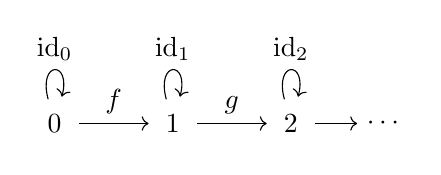
\begin{tikzpicture}[
]
% Objects (circles)
\node[minimum size=0.6cm] (o1) at (0,-1) {0};
\node[minimum size=0.6cm] (o2) at (1.5,-1) {1};
\node[minimum size=0.6cm] (o3) at (3,-1) {2};
\node (dots) at (4.2,-1) {$\cdots$};

% Arrows between objects
\draw[->] (o1) -- node[above] {$f$} (o2);
\draw[->] (o2) -- node[above] {$g$} (o3);
\draw[->] (o3) -- (dots);

\draw[->] (o1) edge[loop above] node[above] {$\id_0$} (o1);
\draw[->] (o2) edge[loop above] node[above] {$\id_1$} (o2);
\draw[->] (o3) edge[loop above] node[above] {$\id_2$} (o3);
\end{tikzpicture}
\end{center}

Given a category $\calC$, a $\calC$-indexed set associates each object of
a category with a set. 
Let's consider a concrete $\calC$-indexed set called $F$.
We can draw $F$ as a ``balloon picture'' like this:

\begin{center}
  \includegraphics[width=175px]{fig/balloon-1.png}
\end{center}

Above each object is drawn a (in this case, finite) set. 
$F_1$ is the set $\{a, b, c\}$, and $F_2$ is is the set 
$\{d, e\}$. 
In addition to associating each object with a set, 
a $\calC$-indexed set also associates each morphism $X \mor{f} Y$
with a function $F_Y \to F_X$, which we can draw on the balloon 
picture like so:

\begin{center}
\includegraphics[width=175px]{fig/balloon-2.png}
\end{center}

Intuitively, we can see that $F$ is describing a relation between two 
categories: our category of interest $\calC$, and an ``external''
category of sets and functions. This relation is called a \textbf{functor}.
Functors have actions on objects 

% \begin{tikzpicture}[
%   node distance=1.5cm,
%   morphism/.style={-Stealth, thick}
% ]

% % Top row of labels
% \node (v) at (0,2) {$v$};
% \node (c) at (3,2) {$c$};

% % Middle row
% \node (y) at (-1.5,1) {$y$};
% \node (w) at (0,1) {$w$};
% \node (a) at (3,1) {$a$};

% % Bottom row (just above the objects)
% \node (x) at (-1.5,0) {$x$};
% \node (h) at (0,0) {$h$};
% \node (b) at (3,0) {$b$};

% % Objects (circles)
% \node[circle, draw, minimum size=0.6cm] (o1) at (0,-1) {0};
% \node[circle, draw, minimum size=0.6cm] (o2) at (1.5,-1) {1};
% \node[circle, draw, minimum size=0.6cm] (o3) at (3,-1) {2};
% \node (dots) at (4.2,-1) {$\cdots$};

% % Arrows between objects
% \draw[morphism] (o1) -- (o2);
% \draw[morphism] (o2) -- (o3);
% \draw[morphism] (o3) -- (dots);

% \end{tikzpicture}




% \begin{center}
%  \begin{tikzpicture}[]

% % Objects
% \node (A) at (0,0) {$A$};
% \node (B) at (3,0) {$B$};
% \node (C) at (1.5,2.5) {$C$};

% % Identity morphisms (loops)
% \draw[->] (A) edge[loop left] node[left] {$\text{id}_A$} (A);
% \draw[->] (B) edge[loop right] node[right] {$\text{id}_B$} (B);
% \draw[->] (C) edge[loop above] node[above] {$\text{id}_C$} (C);

% % Morphisms between objects
% \draw[->] (A) -- node[below] {$f$} (B);
% \draw[->] (A) -- node[left] {$g$} (C);
% \draw[->] (C) -- node[right] {$h$} (B);
% \node[draw, fit=(A)(B)(C), inner sep=1cm, rectangle] {};
% \end{tikzpicture}
% \end{center}


Throughout this section we will work with an arbitrary category \(\calC\).

\begin{definition}[$\calC$-indexed set]
  A $\calC$-indexed set is a functor $F : \calC^\text{op} \Rightarrow \Set$.
\end{definition}

\begin{example}
  Recall that \(\mathsf{STLC}\) is a category
  whose objects are types and whose morphisms \(A \to B\)
  are terms \(x : A \vdash M : B\) quotiented by \(\beta\eta\)-equivalence.
  For each type \(A\),
  the following defines a \(\mathsf{STLC}\)-indexed set \(\mathsf{Tm}(A)\):
  \begin{align}
  \mathsf{Tm}(B)(A) &= \text{the set of morphisms \(A\to B\)} \\
  \mathsf{Tm}(B)(N : A'\to A)
  &= (x\ofty A \vdash M : B) \mapsto (x'\ofty A' \vdash M[N/x] : B)
  \end{align}
\end{example}
This example is a special case of a canonical kind of \(\calC\)-indexed set.
\begin{definition}
  The \emph{representable \(\calC\)-indexed set at \(X\)}
  is written \(\yo X\) and defined by
  \begin{align}
    (\yo X)(A) &= \text{the set of morphisms \(A \to X\)} \\
    (\yo X)(A)(s : A' \to A) &= (f : A \to X) \mapsto (f \circ s : A' \to X)
  \end{align}
\end{definition}

\begin{definition}
  \sloppy
  Let \(P\) and \(Q\) be \(\calC\)-indexed sets.
  A \emph{\(\calC\)-indexed function}
  from \(P\) to \(Q\),
  written \(\alpha : P \Rightarrow Q\),
  is a family of functions \(\alpha_X : PX \to QX\)
  that ``respects substitution''
  in the sense that \(\alpha_{X'}(x\cdot_P p) = \alpha_X(x)\cdot_p p\).
\end{definition}

\begin{itemize}
\item \(\calC\)-indexed functions can be composed:
  the composition of \(\alpha : Q \Rightarrow R\)
  and \(\beta: P \Rightarrow Q\),
  written \(\alpha\circ\beta : P \Rightarrow R\),
  is defined by \((\alpha\circ\beta)_X = \alpha_X \circ \beta_X\).
\item For each \(\calC\)-indexed set \(P\),
  there is a \(\calC\)-indexed function \(\idt_P : P \Rightarrow P\)
  defined by \(\idt_{P,X} = \left(PX \xrightarrow{\idt_{PX}} PX\right)\).
\end{itemize}
By now you may have noticed that \(\calC\)-indexed sets and functions
look like they ought to form a category. More on this later.

\begin{definition}
  Two \(\calC\)-indexed sets \(P,Q\)
  are \emph{isomorphic}
if there are \(\calC\)-indexed functions \(\alpha : P \Rightarrow Q\)
and \(\beta : Q \Rightarrow P\)
such that \(\alpha\circ\beta=\idt_Q\) and \(\beta\circ\alpha=\idt_P\).
\end{definition}

\begin{definition}
  A \(\calC\)-indexed set \(P\) is \emph{representable}
  if there is an isomorphism \(\alpha : P \cong \yo X : \beta\)
  for some object \(X\) of \(\calC\).
\end{definition}


\chapter{Yoneda III: universal constructions, elements, and properties}

\begin{definition}
  \sloppy
  Given two \(\calC\)-indexed sets \(P\) and \(Q\),
  their \emph{product} \(P\times Q\)
  is the \(\calC\)-indexed set defined by
  \((P\times Q)(X) = P(X)\times Q(X)\),
  with substitution defined by
  \((x,y)\cdot_{P\times Q} p = (x\cdot_P p, y\cdot_Q p)\).
\end{definition}

\begin{proposition}
  Let \(X\) and \(Y\) be two objects of a category \(\calC\).
  An object \(P\) is a product of \(X\) and \(Y\)
  if and only if \(\yo P\) is isomorphic to \(\yo X \times \yo Y\).
\end{proposition}

\begin{definition}
  Given two objects \(X\) and \(Y\) of a category \(\calC\),
  there is a \(\calC\)-indexed set of \emph{closures},
  written \(\mathsf{Clos}(X,Y)\),
  defined by \(\mathsf{Clos}(X,Y)(\Gamma) = \calC(\Gamma\times X, Y)\),
  with substitution defined by
  \[
    \mathsf{Clos}(X,Y)(s : \Gamma'\to \Gamma)(f : \Gamma\times X \to Y)
    = \angled{\gamma',x} \mapsto f \circ \angled{s\circ \gamma', x}
  \]
  on generalized elements.
\end{definition}

\begin{proposition}
  Let \(X\) and \(Y\) be two objects of a category \(\calC\).
  An object \(E\) is the exponential \(Y^X\)
  if and only if \(\yo E\) is isomorphic to \(\mathsf{Clos}(X,Y)\).
\end{proposition}

\begin{proposition}
  Suppose the \(\calC\)-indexed set \(P\) is represented
  by the object \(X\).
  Then there exists an element \(u \in PX\),
  called the \emph{\(P\)-universal element},
  which satisfies the following \emph{universal property}:
  for any object \(\Gamma\) and any element \(g \in P\Gamma\),
  there exists a unique morphism \(\hat g : \Gamma \to X\)
  such that \(g = u \cdot_P \hat g\).
\end{proposition}

\begin{itemize}
\item In the case of the product, with \(\yo P \cong \yo X \times \yo Y\),
  the universal element is an element \(u \in \calC(P,X) \times \calC(P,Y)\),
  which is a pair of morphisms \(P\to X, P\to Y\).
  The universal property of this pair is that any other pair \(\Gamma \to X,\Gamma\to Y\)
  factors uniquely through it---precisely the universal property of products
\item In the case of exponents, with \(\yo E \cong \calC(A\times(-),B)\),
  the universal element is an element \(u \in \calC(A \times E,B)\),
  which is a morphism \(A \times E \to B\).
  The universal property of this morphism is that any other morphism
  \(A \times \Gamma \to B\)
  factors uniquely through it---precisely the universal property of exponents.
\end{itemize}

\chapter{Yoneda IV}

%% - Grothendieck universes
%% - The category Set
%% - Functors; opposite categories; C-indexed sets as functors
%% - Natural transformations; C-indexed functions as natural transformations
%% - The Yoneda lemma (without showing naturality in P,c)

%% \begin{itemize}
%% \item Functors form a category where morphisms are natural transformations \begin{itemize}
%%     \item Natural transformations as homotopies between diagrams
%%       (the \(C\to D^\to\) example revisited)
%%     \item Natural transformations as polymorphic maps
%%   \end{itemize}
%% \item Definition of Yoneda embedding
%% \item Restatement of universal properties from previous week in terms of Yoneda embedding
%% (e.g., for products, \(\yo(a\times b) \cong \yo(a)\times \yo(b)\).)
%% \item Yoneda embedding full and faithful. Use this to quickly prove some basic facts:
%%   associativity and commutativity of sums and products, distributivity of products over sums,
%%   ...
%%   These imply type isomorphisms in STLC and Set, entailments of propositional logic.
%% \item Yoneda preserves limits.
%%   This gives a quick proof that all limits can be constructed from products and equalizers.
%%   From this we can compute limits in STLC (it won't have all of them
%%   but it will have some).
%% \end{itemize}

%% \todo: \begin{itemize}
%% \item Slice over c is category of elements of yo c
%% \end{itemize}

\chapter{Monoidal Categories}

\section{Categorifying Monoids}

We have been working thus far with typed PLs, specified using 
typing rules. We used categories to give them semantics and 
diagrams to depict the categories. We will now discuss PLs 
with resources, and use \emph{monoidal categories} to give 
them semantics, and use string diagrams to depict them.

First, let us recall the definition of monoid:


\begin{definition}[monoid]
    A triple $(M, \cdot, e)$ is a monoid if it satisfies:
    \begin{enumerate}
        \item \textbf{Associativity}: $\forall x, y, z \in M
            \,.\, (x \cdot y) \cdot z = x \cdot (y \cdot z)$
        \item \textbf{Identity}: $\forall x \in M \,.\,
            e \cdot x = x = x \cdot e$
    \end{enumerate}
\end{definition}

We have seen one way of categorifying monoids: construct a cateogry 
with one object and a morphism for each element of the monoid.
The monoid operation then corresponds to sequential composition 
and the monoid axioms correspond to the category axioms.

What if we instead categorify monoids by making the \emph{objects} form
a monoid and where the monoid operation corresponds to some notion
of parallel composition. Such categories are called 
\emph{monoidal categories}.
Monoidal categories are a category \(\mathcal{C}\) together with an
operation \(\otimes\), called the tensor product, and a distinguished
object \(I\). The axioms are then encoded as a certain relationship
between corresponding objects. Formally:

% For the axioms, we need a way to relate objects: 1.
% associativity:
% \((A \otimes B) \otimes C \leftright A \otimes (B \otimes C)\) 2.
% identity: \((I \otimes A) \leftright A \leftright (A \otimes I)\)

\begin{definition}[monoidal category]
    A category \(\mathcal{C}\) is a monoidal category if: 
    \begin{enumerate}
        \item there exists a bifunctor \(\otimes: 
            \mathcal{C} \times \mathcal{C} \to \mathcal{C}\)
        \item there exist natural isomorphisms:
            \begin{itemize}
                \item \( \alpha_{A, B, C} : A \otimes (B \otimes C) 
                    \Rightarrow (A \otimes B) \otimes C \)
                \item \( \lambda_{A} : I \otimes A \Rightarrow A \)
                \item \( \rho_A : A \Rightarrow A \otimes I \)
            \end{itemize}
        \item such that the following diagrams commute:
    \end{enumerate}
    \begin{tikzcd}[column sep=large, row sep=large]
    ((A \otimes B) \otimes C) \otimes D 
      \arrow[r, "\alpha_{A,B,C} \otimes \text{id}_D"] 
      \arrow[d, "\alpha_{A \otimes B,C,D}"'] 
      & (A \otimes (B \otimes C)) \otimes D 
        \arrow[r, "\alpha_{A,B \otimes C,D}"] 
      & A \otimes ((B \otimes C) \otimes D) 
        \arrow[d, "\text{id}_A \otimes \alpha_{B,C,D}"] \\
    (A \otimes B) \otimes (C \otimes D) 
      \arrow[rr, "\alpha_{A,B,C \otimes D}"'] 
      & & A \otimes (B \otimes (C \otimes D))
    \end{tikzcd}

    \begin{tikzcd}[column sep=huge]
    (A \otimes I) \otimes B 
      \arrow[rr, "\alpha_{A,I,B}"] 
      \arrow[dr, "\rho_A \otimes \text{id}_B"'] 
      & & A \otimes (I \otimes B) 
        \arrow[dl, "\text{id}_A \otimes \lambda_B"] \\
      & A \otimes B &
    \end{tikzcd}
\end{definition}

The conditions that these diagrams commute are often simply referred 
to as ``coherence conditions.'' The intuition is that the 
three natural isomorphisms need to 
interact with each other well in the sense that if we take any 
two paths between objects, then they are equivalent. 
Proving those two diagrams commute is sufficient to prove the 
\emph{coherence theorem}, which makes the notion described 
above precise.

Let us define some of the other terms in the definition:

\begin{definition}[bifunctor]
A functor from the product category \(\mathcal{C} \times \mathcal{C}\) 
to \(\mathcal{C}\).
\end{definition}

\begin{definition}[natural isomorphism]
natural isomorphism: a natural transformation \(\eta : F \Rightarrow G\)
is a natural isomorphism if for every object \(X \in \mathcal{C}\), the
component \(\eta_X\) is an isomorphism. More concretely, we have the
following diagram for every $f : X \to Y$ in $\mathcal{C}$:

\begin{tikzcd}[column sep=large, row sep=large]
F(X) 
  \arrow[r, bend left=30, "\eta_X"] 
  \arrow[d, "F(f)"'] 
  & G(X) 
    \arrow[l, bend left=30, "\eta_X^{-1}"] 
    \arrow[d, "G(f)"] \\
F(Y) 
  \arrow[r, bend left=30, "\eta_Y"'] 
  & G(Y) 
    \arrow[l, bend left=30, "\eta_Y^{-1}"]
\end{tikzcd}
\end{definition}


\section{examples}

\subsection{monoids}

Given any monoid \((M, \cdot, e)\) whose objects are the elements of
\(M\) and whose morphisms are only the identities. The tensor product on
objects \(a, b\) is just the monoid operation. Then the tensor product
of morphisms just gives the corresponding identity morphism.

We must show that the \(\otimes\) defines a functor: - it clearly
respects identity by the definition above - showing it respects
composition amounts to proving the following:
\((f_1 \otimes f_2) \circ (g_1 \otimes g_2) =  g_1 \circ g_1 \otimes f_2 \circ g_2\).
This holds because all morphisms are the identity - by the monoid laws,
the objects we need to define natural transformations between are
exactly equal, so we just define the transformations to be the identity
on each component.

\hypertarget{real-numbers}{%
\subsection{real numbers}\label{real-numbers}}

Consider the preorder of real numbers viewed as a category. We can
define the tensor product on objects to be addition and the monoidal
unit to be 0. Given two morphisms \(n_1 \to n_2\), \(m_1 \to m_2\), the
tensor product is the morphism \(n_1 + m_1 \to n_2 + m_2\), which we
know exists by monotonicity of addition. Similar to the monoid example,
the natural isomorphisms are the identity on each component because the
corresponding objects are equal.

\hypertarget{string-diagrams}{%
\subsection{string diagrams}\label{string-diagrams}}

In string diagrams, we represent objects with wires, morphisms with
boxes (including an identity). Sequential compositions correspond to
wiring boxes together. Tensor product for objects corresponds to
juxataposing wires next to each other, and tensor products of wires is
putting boxes next to each other. The monoid unit corresponds to a
``phantom wire'' which need not be drawn.

In any monoidal category, we have a notion of ``generating objects and
morphisms,'' which can't be decomposed into the tensor product of other
objects; the category is then formed by taking all the possible tensor
products.

Many of the laws correspond to extremely intuitive facts about diagrams:
(picture).

\hypertarget{real-numbers-1}{%
\subsection{real numbers}\label{real-numbers-1}}

Here, we have diagrams representing proofs of \(v+x \le y\),
\(w + u \le x + y\), \(t \le v + w\). We can then wire the boxes
together to get a proof of \(t + u \le y + z\) (fig.~4)

\hypertarget{symmetric-monoidal-categories}{%
\section{symmetric monoidal
categories}\label{symmetric-monoidal-categories}}

Notice that in this category, we have that the tensor product is
commutative. The categories where this holds are called \emph{symmetric
monoidal categories}, which come equipped with an additional natural
transformation \(\gamma : A \otimes B \Rightarrow B \otimes A\). We get
the following laws: (Fig. 5)

\hypertarget{example-cartesian-categories}{%
\section{example: cartesian
categories}\label{example-cartesian-categories}}

If \(\mathcal{C}\) has a product \(\times\) and terminal object \(T\),
then this forms a monoidal category with \(\otimes = \times\) and
\(I = T\).

The natural isomorphism for associativity was proven in Homework 1:
\(\alpha = \langle \langle \pi_1, \pi_1 \circ \pi_2 \rangle, \pi_2 \circ \pi_2 \rangle\).
We also have \(\lambda = \pi_1\) and
\(rho = \langle \star, \text{id}_A \rangle\).

In the typed PL perspective, we had rules for operating with products
and the terminal object: (pair intro, unit intro).

We might ask given terms \(x : A \vdash M : B\) and
\(\langle x, y \rangle : A \times B \vdash N : C\), how can we construct
a term \(T\) such that \(x : A \vdash T : C\)? We can do this with our
term language. We can also do it in string diagrams: (fig.~6). Doing
this requires a \emph{copy} operation, which allows us to duplicate
\(A\).

In general, monoidal categories won't always have a copy operation. This
corresponds to the intuition of monoidal categories as representing
resources -- if our resource can be copied, then our category would have
a copier. If not, then it wouldn't.

Often, when we have a copy operation, we also have a discard operation:
(draw it). These operations will satisfy the following rules: (fig.~7)

\chapter{Limits and colimits}
So far, we've been building a ``categorical dictionary'' of structure that
categories might have that makes them useful models for programming languages.
Categorical products let us model products in programming languages, exponential
objects let us model higher-order functions. Limits and colimits take these
ideas to their extreme: we will see that a category that has limits and colimits
has a rich vocabulary of universal constructions of which products and
exponentials are a special case. The utility of limits and colimits is in their 
generality, both in the kinds of constructions they give you and also how they
are characterized. We will see that limits are \emph{preserved} or
\emph{created} by the presence of certain functors, enabling us to characterize
a large amount of categorical structure with relatively little work. 

As an example of how limits generalize products, let
\[
\mathsf{Point} = \{
x: \R, y: \R, z: \R
\}
\]
This leads to the idea of indexed products.
\begin{definition}[Indexed product]
  \sloppy
  Let \((X_i)_{i\in I}\) be an \(I\)-indexed
  family of objects of a category \(\calC\).
  An \emph{indexed product} of \((X_i)_{i\in I}\)
  consists of an object \(P\)
  and a family of morphisms \((\pi_i : P \to X_i)_{i\in I}\)
  satisfying the following universal property:
  for any object \(Y\)
  and any family of morphisms \((f_i : Y \to X_i)_{i\in I}\),
  there exists a unique morphism \(\angled{f_i}_{i\in I} : Y \to P\)
  such that \(\pi_i \circ \angled{f_i}_{i\in I} = f_i\) for all \(i\) in \(I\).
\end{definition}
While records are typically finite, the definition of indexed product
works just as well for infinite products.
For example,
\begin{proposition}
  \(1\) is the indexed product of \((k)_{k\in \N}\)
  in the category of natural numbers under divisibility.
\end{proposition}
More generally, indexed products in preorders are like infima.

Indexed products are in some sense the ``largest'' way to map
into a tuple of objects.
For example, the product for \(\mathsf{Point}\)
is the ``largest'' way of filling in the question marks in this diagram:
\[% https://tikzcd.yichuanshen.de/#N4Igdg9gJgpgziAXAbVABwnAlgFyxMJZABgBoBGAXVJADcBDAGwFcYkQAdDgJRAF9S6TLnyEU5CtTpNW7LrwFDseAkQBMkmgxZtEnHv0EgMy0UQnEp22XoD8-KTCgBzeEVAAzAE4QAtkgBmGhwIJDJpHXZ7GkZ6ACMYRgAFYRUxEC8sZwALHENPH39EIJAQpAkImxB7RRBvP0Dg0MQNSt1qhz4gA
\begin{tikzcd}
   & ? \arrow[ld, "?"'] \arrow[d, "?"] \arrow[rd, "?"] &    \\
\R & \R                                                & \R
\end{tikzcd}\]
Similarly, \(1\) is the ``largest'' way to fill in
the question marks in this diagram:
\[% https://tikzcd.yichuanshen.de/#N4Igdg9gJgpgziAXAbVABwnAlgFyxMJZARgBpiBdUkANwEMAbAVxiRAH4QBfU9TXfIRQAGUsKq1GLNsW68QGbHgJEy46vWatEIAExy+SwUV1iJm6ToDMBhf2VDkVsxqnaQAHQ9QIOBFwkYKABzeCJQADMAJwgAWyRREBwIJDJJLTZOHkiY+MRE5KRTdMsOW2i4hOpCxGcS9yz5CryClMQAFlcMnU5qBjoAIxgGAAV7Yx0orGCACxxuCi4gA
\begin{tikzcd}
1 & 2                                                                  & 3 & \dots \\
  & ? \arrow[lu, "?"] \arrow[u, "?"] \arrow[ru, "?"] \arrow[rru, "?"'] &   &
\end{tikzcd}\]

All of these diagrams are ``discrete'': they consist only of objects,
with no morphisms connecting them.
More generally, we can ask if it is possible to find the largest
way of mapping into an arbitrary diagram consisting of both objects and morphisms.
This is called a \emph{limit}.

To be more precise about this, it is useful to give a formal definition of 
what a diagram is:
\begin{definition}[Diagram]
  \sloppy
  For two categories $\calI$ and $\calC$, a
  \emph{diagram of shape $\calI$} is a functor $F : \calI \to \calC$.
  The category $\calI$ is called the \emph{shape of the diagram}.
\end{definition}

It is typical for the shape of a diagram to be a simple discrete category with
only a few objects and morphisms.  For example, we can consider $\calI = \bullet
\quad \bullet$; then, a diagram of shape $\calI$ in some category $\calC$ would
pick out a pair of two objects in $\calC$. Here is a simple example of a
diagram:

\begin{center}
  \includegraphics[width=100px]{fig/diagram-1.png}
\end{center}

The essential idea of a limit is that it that it is the largest way of ``mapping 
into a diagram''. 
The way to formalize this is via the notion of a \emph{cone}:

\begin{definition}[Cone]
  \sloppy
  Let \(D : \mathcal I \to \calC\) be a diagram of shape \(\mathcal I\)
  in a category \(\calC\).
  A \emph{cone} over \(D\) is a pair \((P,p)\)
  where \(P\) is an object of \(\calC\)
  and \(p\) is a family of morphisms \((p_i : P \to D(i))_{i\in I}\)
  such that \(D(f) \circ p_i = p_j\) for all morphisms \(f : i \to j\)
  of \(\mathcal I\).
\end{definition}

Let's understand this definition for the simple diagrams of shape $\calI =
\bullet \quad \bullet$ before we consider more more interesting shapes with
morphisms in them. In the above example diagram, the tuple $(P, p)$
is a cone where $p_L = f$ and $p_R = g$.


\begin{definition}[Limit]
  Let \(D : \mathcal I \to \calC\) be a diagram of shape \(\mathcal I\)
  in a category \(\calC\).
  A \emph{limit} of \(D\) is a terminal cone.
\end{definition}



\section{Examples of limits}

We have seen two examples of limits already, in the homework.
\begin{itemize}
\item Given two morphisms \(X \mor{f} Z \xleftarrow{g} Y\),
  the \emph{pullback} is the largest way of mapping into \(f,g\),
  in other words the largest way of filling in the question marks in this
  diagram:
  \[
  % https://tikzcd.yichuanshen.de/#N4Igdg9gJgpgziAXAbVABwnAlgFyxMJZABgBoBGAXVJADcBDAGwFcYkQANEAX1PU1z5CKcqWLU6TVuwCaPPiAzY8BIqKo0GLNohAAtef2VCiZcZqk6QAfh4SYUAObwioAGYAnCAFskAZhocCCQySW12WxpGegAjGEYABQEVYRAPLEcACxxDEE8ff0DgxFEw6V1bXncvXxKipAAmC3DdR1z82tCgxubyvJAo2Pik41VddKyc7kpuIA
\begin{tikzcd}
? \arrow[d, "?"'] \arrow[r, "?"] & Y \arrow[d, "g"] \\
X \arrow[r, "f"']                & Z
\end{tikzcd}
  \]
  Explicitly, a pullback is a 3-tuple \((W,p,q)\)
  where \(p : W \to X\) and \(q : W \to Y\)
  and \(fp = gq\)
  satisfying the following universal property:
  for any other 3-tuple \((W',p',q')\)
  where \(p' : W' \to X\) and \(q' : W' \to Y\)
  and \(fp' = gq'\),
  there exists a unique morphism \(w : W' \to W\)
  such that \(pw = p'\) and \(qw = q'\).
  \[% https://tikzcd.yichuanshen.de/#N4Igdg9gJgpgziAXAbVABwnAlgFyxMJZARgBoAmAXVJADcBDAGwFcYkQANEAX1PU1z5CKcqWLU6TVuwCaPPiAzY8BIqKo0GLNohAAtef2VCiZcZqk6QAdUOKBK4cgAMpZxK3Td1gOQ8JMFAA5vBEoABmAE4QALZIAMw0OBBIrpLa7GggNIz0AEYwjAAKDia6kVhBABY4dlGxCUkpiGTpXiAAjnXRcS1NSKJtVkHdDYhpyQMWGbrh2SC5BcWlquWVNaO9ACz94zQFYFBIALTxaZ5WXTn5hSXGqyAV1bW8ET1IOyCTfSAHR4hnabtDp+V4gerbXaJIbsADu-m4QA
\begin{tikzcd}
W' \arrow[rdd, "q"', bend right] \arrow[rrd, "q'", bend left] \arrow[rd, "w"] &                                  &                  \\
                                                                              & W \arrow[d, "p"'] \arrow[r, "q"] & Y \arrow[d, "g"] \\
                                                                              & X \arrow[r, "f"']                & Z
\end{tikzcd}\]
\item Given two morphisms \(% https://tikzcd.yichuanshen.de/#N4Igdg9gJgpgziAXAbVABwnAlgFyxMJZABgBpiBdUkANwEMAbAVxiRAA0QBfU9TXfIRQBGclVqMWbAJrdxMKAHN4RUADMAThAC2SMiBwQkokHAAWWNTmPV6zVohCKQ1BnQBGMBgAV+eAmwaWIpm1jzqWrqI+oY2EvZsai6mFlZIALTCXBRcQA
\begin{tikzcd}
X \arrow[r, "g"', shift right] \arrow[r, "f", shift left] & Y
\end{tikzcd}\),
their \emph{equalizer} is the largest way of mapping into \(f,g\)
in other words the largest way of filling in the questino marks in this
diagram:
\[% https://tikzcd.yichuanshen.de/#N4Igdg9gJgpgziAXAbVABwnAlgFyxMJZABgBoBGAXVJADcBDAGwFcYkQANEAX1PU1z5CKAEwVqdJq3YBNHnxAZseAkXKliEhizaIQAfh4SYUAObwioAGYAnCAFskZEDghJ1IOAAssVnO5ptaT1TEBpGegAjGEYABQEVYRAbLFMvf15rO0dEZ1cAyR12KzDPHz8kAFpyTJBbByQxFzdcwKldA1KI6LiEoXYUtIyFepym-MQPII7DbkpuIA
\begin{tikzcd}
                                                            & ? \arrow[ld, "?"'] \arrow[rd, "?"] &   \\
X \arrow[rr, "g"', shift right] \arrow[rr, "f", shift left] &                                    & Y
\end{tikzcd}\]
Explicitly, the equalizer is a 3-tuple \((W,p,q)\)
where \(p : W \to X\) and \(q : W \to Y\)
and \(fp = q\) and \(gp = q\)
satisfying the following universal property:
for any other 3-tuple \((W',p',q')\)
where \(p' : W' \to X\) and \(q' : W' \to Y\)
and \(fp' = q'\) and \(gp' = q'\)
there exists a unique \(w : W' \to W\)
such that \(pw = p'\) and \(qw = q'\).
\[% https://tikzcd.yichuanshen.de/#N4Igdg9gJgpgziAXAbVABwnAlgFyxMJZABgBoAmAXVJADcBDAGwFcYkQANEAX1PU1z5CKchWp0mrdgE0efEBmx4CRAIylV4hizaIQAdTn8lQtaWJbJugwHIe4mFADm8IqABmAJwgBbJGRAcCCR1EDgACyx3HBCabSk9JxAaRnoAIxhGAAUBZWEQTywncJjeD28-RACg2IkddndksMjopABaVTKQL18kUUDgqrirdjQm1Izs3NM9QuLS+R7K-prEUPjrAEcjboqkAGYaVYCN0bsU9MyckxVZopKmjLAodv3iLqWDo8H1kb1N84gJ4vRBvD57UHfPrDep6ADu9m4QA
\begin{tikzcd}
                                                            & W' \arrow[ldd, "p'"', bend right] \arrow[rdd, "q'", bend left] \arrow[d, "w"] &   \\
                                                            & W \arrow[ld, "p"'] \arrow[rd, "q"]                                            &   \\
X \arrow[rr, "g"', shift right] \arrow[rr, "f", shift left] &                                                                               & Y
\end{tikzcd}\]
This definition can be simplified a bit:
notice that in the 3-tuple \((W,p,q)\),
the morphism \(q\) is forced to be \(fp\).
So it is equivalent to say that an equalizer
is a 2-tuple \((W,p)\)
such that \(fp = gp\),
which satisfies the universal property
that for any other \((W',p')\)
with \(fp' = gp'\), there exists a unique \(w : W' \to W\)
such that \(wp = p'\) and \(wq = q'\).
\[% https://tikzcd.yichuanshen.de/#N4Igdg9gJgpgziAXAbVABwnAlgFyxMJZARgBpiBdUkANwEMAbAVxiRAA0QBfU9TXfIRQAmclVqMWbAJrdeIDNjwEiABjHV6zVohAB1OXyWC1pVeK1TdegOTdxMKAHN4RUADMAThAC2SdSA4EEhkEtps7iDUcAAWWO44SAC0xDwe3n6IAUEhmpI6IE5RILHxiYihDHQARjAMAAr8ykIgnlhOMYlpIF6+SKKBwVl54bpohj0ZSADM1DnDYVYKdt29mbOD-SNLAO7FVbUNTSa6bR1dFFxAA
\begin{tikzcd}
W' \arrow[rd, "p'"] \arrow[d, "w"'] &                                                           &   \\
W \arrow[r, "p"]                    & X \arrow[r, "f", shift left] \arrow[r, "g"', shift right] & Y
\end{tikzcd}\]
\end{itemize}

The equalizer looks like a refinement type:
\[
\text{equalizer of }
\begin{tikzcd}
X \arrow[r, "g"', shift right] \arrow[r, "f", shift left] & Y
\end{tikzcd}
\qquad\leadsto\qquad
\{x : X \mid f(x) = g(x)\}
\]

The pullback looks like a ``fiber product'':
\[\includegraphics[width=100px]{fig/pb.png}\]


\subsection{Some important facts}

\begin{proposition}
  A category with all products and a terminal objects has all limits.
\end{proposition}

\begin{proposition}
  Every limit is an equalizer of a product.
\end{proposition}

\begin{proposition}
  Any full and faithful functor preserves limits and colimits.
  Consequently,
  the Yoneda embedding preserves these as well.
\end{proposition}

\section{Colimits}
\chapter{Adjunctions}

\begin{itemize}
  \item So far we've mostly focussed on characterizing properties 
  of an individual category. Now let's broaden our focus to discuss 
  in more detail
  relationships between categories.
  \item First, let's study the strongest possible relationship between
  two categories: does it mean for two categories to be equivalent? 
  Following intuition from set isomorphism, we will want to design 
  two functors between the categories that behave like inverses.
  \item For this definition we will need a way of talking equivalence 
  of functors:
  \begin{definition}[Natural isomorphism of functors]
    Let $\calC$ and $\calD$ be categories and $F, G : \calC \to \calD$ 
    be functors. Then, $F$ and $G$ are \emph{naturally isomorphic},
    written $F \cong G$, if there is a natural transformation $\alpha : F \Rightarrow G$
    whose components are isomorphisms.

  \end{definition}
  % todo: make this just be X x Y

  % \begin{example}
  %   Let $\calC$ be the preorder category on natural numbers, and let 
  %   $\calD$ be a category whose objects are pairs of natural numbers 
  %   and where there is a morphism $(x,y) \to (z, w)$
  %   if and only if $x \le z$ or $y \le w$.

  %   Then, let $F : \calC \to \calD$ be $F = X \mapsto (0, X)$  and 
  %   $G : \calC \to \calD$ be $G  = X \mapsto (X, 0)$. Then,
  %   these two functors are naturally isomorphic along the natural 
  %   transformation
  %   $\alpha : F \Rightarrow G$ where components $\alpha_X : F(X) \to G(X)$
  %   swap the order of tules, $\alpha_X = (0, X) \to (X, 0)$.
  % \end{example}

  \item Now, to give an equivalence of categories, we must show that there exists a pair of functors $F$ and 
  $G$ between them whose compositions are naturally isomorphic to 
  the identity functors on each category:
  \begin{definition}[Equivalence of categories]
    \sloppy
    Let $\calC$ and $\calD$ be categories. Then, $\calC$ is equivalent
    to $\calD$, written $\calC \cong \calD$, if there are two functors 
    $F : \calC \to \calD$ and $G: \calC \to \calD$ satisfying
    $F \circ G \cong \id_\calC$ and $G \circ F \cong \id_\calD$, where $\id_\calC$ 
    and $\id_\calD$ are the identity functors on $\calC$ and $\calD$ respectively.
  \end{definition}
  \item There are some surprising categorical equivalences that are worth 
  thinking about:
  \begin{proposition}
    The category of finite pointed sets $\mathsf{FinSet}^*$ is equivalent to the category 
    of finite sets and partial functions $\mathsf{FinSet}_\text{par}$. 
  \end{proposition}

  The intuition behind this equivalence is interesting. First let's identify 
  the functors that form the equivalence. Let $F :
  \mathsf{FinSet}_\text{par} \to \mathsf{FinSet}^*$. The action 
  on objects is straightforward: $F(X) = (X \uplus \{\star\}, \star)$
  i.e., $F$ sends a set $X$ to a pointed set with $X$ extended by 
  some element $\star$ with $\star$ as the point.
  The action on morphisms is interesting. Let $f : X \to Y$ be a partial 
  function. Then, we define:
  \begin{align*}
    F(f) &: (X \uplus \{\star\}, \star) \to (Y \uplus \{\star\}, \star) \\
    &= x \mapsto \begin{cases}
      \star \quad& \text{if }f(x)~\text{undefined} \\ 
      f(x) \quad& \text{otherwise.}
    \end{cases}
  \end{align*}
  Intuitively, the $\star$ stands in for the subset of $X$ on which $f$ is undefined.
  The inverse $G$ is also straightforward: its action on objects is to 
  forget remove point, $G((X, \star)) = X \setminus \star$. Then, its action on morphisms
  map the point to undefined:
  \begin{align*}
    G(g) &: X \setminus \star \to Y \setminus \star \\ 
    &= x \mapsto 
    \begin{cases}
      \bot \quad&\text{if }g(x) = \star \\
      g(x) \quad&\text{otherwise}
    \end{cases}
  \end{align*}

  Now, show that there is a natural isomorphism $\alpha : F \circ G \Rightarrow \id_{\textsf{FinSet}^*}$.
  This is not too hard and a good exercise. 
  It requires showing that there is a $\mathsf{FinSet}^*$ isomorphism 
  $(X, a) \cong ((X \setminus a) \uplus \star, \star)$. 

  \item Categorical equivalences are very powerful when they arise but 
  the condition is often too strong. 
  A natural weakening of this notion will be an \emph{adjunction}, which will be pairs of 
  functors between categories are a form of ``weak equivalence''. 

  \item The natural notion of weakening here will be as follows. Let $\calC$ and $\calD$ 
  be categories and $F : \calC \to \calD$ and $G : \calD \to \calC$ be functors. 
  Then, instead of requiring that round-trips of $F$ and $G$ be naturally isomorphic identity functors, 
  an adjunction will require instead that there simply exist some pair of natural transformations:
  \begin{align}
    \eta : \id_\calC \Rightarrow G \circ F  \qquad
    \epsilon :  F \circ G \Rightarrow \id_\calD 
    \label{eq:adjoint-units}
  \end{align}

  The natural transformation $\eta$ is called the \textbf{unit} of the adjunction and 
  $\epsilon$ is called the \textbf{counit}, the functor $F$ is called 
  the \textbf{left adjoint}, and the functor $G$ the \textbf{right adjoint}.

  \item There is one more coherence requirement we place on these natural
  transformations in order for them to form an adjunction. But, before we do
  that, let's examine this notion of notion of ``weak equivalence'' in a 
  simple preorder category to understand what it means before we give the 
  full definition of adjoint functors for general categories.
\end{itemize}

\section{Adjunctions for preorder categories: Galois connections}
\begin{itemize}
  \item As usual it's very useful to study new category theory definitions in 
  pre-order categories to gain order-theoretic intuition about them before 
  generalizing to the general setting where there can be more than one morphism 
  between any two objects.
  
  \item Let $(X, \le_X)$, $(Y, \le_Y)$ be preorders. Recall that a \emph{monotone map}
  is a function $f : X \to Y$ that respects the preorder, i.e., 
  if $x_1 \le_X x_2$ then $f(x_1) \le_Y f(x_2)$. Recall that functors between 
  preorder categories are exactly monotone maps.

  \item Let's interpret the definition of adjoint in this setting. First, 
  let's give two example functors between two preorder categories:

  % https://tikzcd.yichuanshen.de/#N4Igdg9gJgpgziAXAbVABwnAlgFyxMJZABgBpiBdUkANwEMAbAVxiRAB12BbOnACwDGjYABEAviDGl0mXPkIoAjOSq1GLNgEFJ0kBmx4CRAEwrq9Zq0QgAQjpkH5RAMxm1ltgGF7e2YYUkpIqqFhrWnDz8QgzAnhJSDnJGSkEh6lYgij76SQGmwebpbMbZfk4orgXuYSDOpY7JyAAsbqEZIvW5RC1VbWxNkqowUADm8ESgAGYAThBcSMogOBBIxgkgM3Or1MtIzuub84gArDsriABsB7NHF2dIAOzXW4iuS+cAHM9HD-eIAJzfBZ-O4gABGMDAUCQxCBlz+pnBkOhr1hukO23eSFBEKhezRUxuSFOWMQiNxKIJGyJiF+pK+6Jp-z+H2oFPxcLeuwBcNZpOZSLxqLEFDEQA
\begin{tikzcd}
  \mathcal{D} & A \arrow[r] \arrow[red, rd] & B \arrow[r] \arrow[red, dr, bend left] & C \arrow[red, d] \\
  \mathcal{C} & 1 \arrow[r] \arrow[blue, u] & 2 \arrow[r] \arrow[blue, ul, bend left] & 3 \arrow[blue, ul]
  \end{tikzcd}

  Here we've drawn $F : \calC \to \calD$ in blue and $G : \calD \to \calC$ in red.

  \item Let's check if these functors satisfy the adjoint requirement as we've seen it 
  so far. First, let's try to find a unit by finding a natural transformation
  $\eta : \id_\calC \Rightarrow G \circ F$. 
  Then, $\eta$ is a $\calC$-indexed family of morphisms in $\calC$:
  \begin{align*}
    \eta_1 = 1 \to 2 \quad \eta_2 = \id_2 \quad \eta_3 = \id_3
  \end{align*}

  We can also build the counit, which is a $\calD$-indexed family of morphisms in $\calD$:

  \begin{align*}
    \epsilon_A = \id_A \quad \epsilon_B = \id_B \quad \epsilon_C = B \to C 
  \end{align*}

  Intuitively, these two natural transformations are characterizing what happens 
  after round trips of following $F$ and $G$. The unit $\eta$ says that, after 
  following a round trip of $F$ and then $G$, we must end up ``in a higher place'' than we started;
  dually, the counit $\epsilon$ is saying that after a round trip of $G$ then $F$ 
  we must end up ``in a lower place'' than we started.

  \item Now we can reverse engineer an order-theoretic understanding for the 
  unit and the counit of the adjunctions $F$ and $G$.
  This relationship has a name in order theory:

  \begin{definition}[Galois connection]
    Let $(X, \le_X)$ and $(Y, \le_Y)$  be preorders and let $\alpha : X \to Y$ 
    and $\gamma : Y \to X$ be monotone functions. Then, $\alpha$ and 
    $\gamma$ form a \emph{Galois connection} if, for all $x \in X$ and $y \in Y$:
    \begin{align*}
      x \le \gamma(\alpha(x))  \qquad \text{and} \qquad \alpha(\gamma(y)) \le y
    \end{align*}
  \end{definition}

  \item Pause for a moment to absorb how close a Galois connection is to an inverse. 
  If $\gamma$ and $\alpha$ above were inverses, then indeed this would be 
  an inverse.

  \item An equivalent definition to the above is that, for all $x \in X, y \in Y$, 
  it holds that:
  \begin{align}
    \alpha(x) \le y \text{ if and only if } x \le \gamma(y)
    \label{eq:galois-hom}
  \end{align}

  Exercise: Why is this equivalence true? 

  \item A programming languages example: Galois connections are important in defining 
  abstract interpreters. The map $\alpha$ is called the \emph{abstraction function} and 
  $\gamma$ is called the \emph{concretization function}, and $\alpha$ is left adjoint to $\gamma$.



\end{itemize}

\subsection{Adjoints preserve structure}
\begin{itemize}
  \item An important property of adjoints is that left adjoints preserve colimits 
  and right adjoints preserve limits. This property is of course true for 
  Galois connections, so let's see what it means in that setting first:
  \begin{theorem}
    Let $(X, \le)$ and $(Y, \le)$ be complete partial orders (i.e., they both have all 
    meets and joins) and let $\alpha : X \to Y$ and $\gamma : Y
    \to X$ be monotone functions where $\alpha$ is left adjoint to $\gamma$. Then,
    for any $x_1, x_2 \in X$ we have that:
    \begin{align}
    \alpha(x_1 \sqcup x_1) = \alpha(x_1) \sqcup \alpha(x_2)
    \end{align}
    and, for any $y_1, y_2 \in Y$ we have that:
    \begin{align}
      \gamma(y_1 \sqcap y_2) = \gamma(y_1) \sqcap \gamma(y_2)
    \end{align}
  \end{theorem}
  \begin{proof}
    Let's prove that the left adjoint preserves meets; the other 
    one is a good exercise.
    By monotonicity, $\alpha(x_1) \sqcup \alpha(x_2) \le \alpha(x_1 \sqcup x_2)$. 
    So, we need to show $\alpha(x_1 \sqcup x_2) \le \alpha(x_1) \sqcup \alpha(x_2)$.
    We will use \cref{eq:galois-hom} to show this. 
    Let $m = x_1 \sqcup x_2$ and $m^* = \alpha(x_1)\sqcup \alpha(x_2)$. Then,
    \begin{align*}
      \alpha(m) \le m^* \iff m \le \gamma(m^*)
    \end{align*}
    Proceeding on the right hand side, 
    we use the fact that $\gamma$ is monotone to build an intermediate inequality:
    \begin{align*}
    \gamma(\alpha(x_1)) \sqcup \gamma(\alpha(x_2)) \le \gamma(\alpha(x_1)\sqcup \alpha(x_2))
    \end{align*}

    So, if we can show $x_1 \sqcup x_2 \le \gamma(\alpha(x_1)) \sqcup \gamma(\alpha(x_2))$, 
    we are done. This follows directly from adjoint closure: $x \le \gamma(\alpha(x))$ for all $x$.
  \end{proof}
\end{itemize}

\section{Adjunctions for preorders, continued}
\marginnote{Notes from John's lecture}
\begin{itemize}
  \item Recall the Galois connection example:

  \begin{center}
  \includegraphics[width=300px]{fig/galois.png}
  \end{center}
  \item We defined a pair of functions $\alpha : \calC \to \calA$
  and $\gamma : \calD \to \calC$, where $\alpha$ is 
  left-adjoint to $\gamma$.
  We defined an example $\gamma$ as follows (shown in red):
   \begin{center}
  \includegraphics[width=300px]{fig/galois-2.png}
  \end{center}
 
  \item To get to the general definition of preorder,
  we will study the properties of $\alpha$ 
  and $\gamma$. We will want our general definition of 
  adjoint to preserve \emph{all} of this structure

  \item What is the property we want $\alpha$ to have, 
  given this definition of $\gamma$? 
  In some sense, it is \emph{the most precise 
  abstraction} would can make.

  \item For example, we can define a really bad $\alpha$ 
  that is very imprecise. For instance, 
  we could let $\alpha(\_) = ?$. But if we did this, 
  then $\alpha$ would \emph{not be an adjoint}.

  \item There is a collection of interesting properties 
  we want $\alpha$ to have so that it is in some 
  sense ``most precise'':
  \begin{enumerate}
    \item $\alpha(c)$ is the smallest $a \in \calA$ 
    such that $c \le \gamma(a)$. 
    \item $\gamma(a)$ is the largest $c \in \calC$ 
    such that $\alpha(c) \le a$.
    \item For all $a \in \calA$ and $c \in \calC$, 
    $\alpha(c) \le a$ if and only if 
    $c \le \gamma(a)$.
  \end{enumerate}

  \item These fun facts are more than just fun facts: they are 
  in fact \emph{equivalent definitions} of adjoints (at least 
  for preorders). 

  \begin{theorem}
    Let % https://tikzcd.yichuanshen.de/#N4Igdg9gJgpgziAXAbVABwnAlgFyxMJZABgBpiBdUkANwEMAbAVxiRAB12BbOnACwDGjYAEEAviDGl0mXPkIoAjOSq1GLNpx78hDYAGEJY1TCgBzeEVAAzAE4QuSMiBwQkykACMYYKEgDMzvTMrIgc7IxofHSS0iB2Du7Urk7U3r4BQeqh4WZ0XDySFGJAA
    \begin{tikzcd}
    \mathcal{C} \arrow[r, "\alpha", bend left] & \mathcal{A} \arrow[l, "\gamma", bend left]
    \end{tikzcd} be a pair of functors. Then the following 
    are equivalent:
    \begin{enumerate}
      \item $\alpha \dashv \gamma$ 
      \item For any $c \in \calC$, $\alpha(c)$ is the 
      smallest $a \in \calA$ such t hat $c \le \gamma(a)$
      \item For any $a \in \calA$, 
$\gamma(a)$ is the largest $c \in \calC$ 
    such that $\alpha(c) \le a$.
    \item For all $a \in \calA$ and $c \in \calC$, 
    $\alpha(c) \le a$ if and only if 
    $c \le \gamma(a)$.
    \end{enumerate}
  \end{theorem}

  \item This is going to be a big proof. First we'll prove 
  that (1) implies (2).

  \todo{} fell behind. Same as the next one really.

  \item If $\alpha \dashv \gamma$ then for all 
  $a \in \calA$, $\gamma(a)$ is the largest 
  $c \in \calC$ such that $\alpha(c) \le a$

  First, $\alpha(\gamma(a)) \le a$, holds by 
  $\alpha \dashv a$

  Now we need to show $\gamma(a)$ is the largest such. 
  Suppose $c \in \calC$ such that $\alpha(c) \le a$. 
  Need to show that $c \le \gamma(a)$. 
  By $\gamma$ is monotone, 
  \begin{align*}
    \gamma(\alpha(c)) \le \gamma(a)
  \end{align*}
  By definition of adjoint, $c \le \gamma(\alpha(c))$, 
  which completes the proof.

  \item Proof that (2) implies (4). 

    For any $c \in \calC$, $\alpha(c)$ is the 
    smallest $a \in \calA$ such t hat $c \le \gamma(a)$.
    Want to show that for all $a \in \calA$, $c \in \calC$, 
    $\alpha(c) \le a \iff c \le \gamma(a)$.

    $(\Rightarrow)$: Have that $\alpha(c) \le a$, 
    need to show that $c \le \gamma(a)$.
    By monotonicity, we have that $\gamma(\alpha(c)) \le \gamma(a)$.
    By assumption, $c \le \gamma(\alpha(c))$.\footnote{Note: 
    cannot appeal to adjoint roundtrip property here. This is the assumption 
    in equivalent condition (2).}

    $(\Leftarrow)$: Have $ c \le \gamma(a)$. Want $\alpha(c) \le a$.
    Define some helpful notation: the \emph{downset} $c \downarrow \gamma = \{a
    \mid c \le \gamma(a) \}$. 
    Let $\varphi(a) = \text{min}(c \downarrow \gamma)$. 
    \todo {get the rest}

    \item Proof that (4) implies (1).
    If for all $a \in \calA, c \in \calC$ 
    it holds that $\alpha(c) \le a$ iff $c \le \gamma(a)$, 
    then
    for all $a \in \calA, c \in \calC$ 
    it holds that $\alpha(\gamma(a)) \le a$ and 
    $c \le \gamma(\alpha(c))$.


    First, show $\alpha(\gamma(a)) \le a$. 
    By assumption this is true if and only if 
    $\gamma(a) \le \gamma(a)$, which vacuously holds.
    The other side is identical.
\end{itemize}

\section{Generalizing beyond preorders}
\begin{itemize}
  \item We want a general definition of adjoints that generalizes the above 
  four-way equivalence. 
  \item To get there, we will first become more formal about 
  this downarrow.
  \item Let $\calC$ and $\calA$ be categories. 
  Then, for an object $c \in \calC$, 
  the category $c \downarrow G$ is a category 
  whose objects are morphisms $c \to G(a)$ for each 
  object $a \in \calA$.
  Morphisms are commuting triangles:\marginnote{This is an 
  instance of a \emph{comma category}.
  Thing of note: notice how the preorder notion of a 
  ``downset'' uses the same notation as comma category.}

  \begin{center}
    % https://tikzcd.yichuanshen.de/#N4Igdg9gJgpgziAXAbVABwnAlgFyxMJZABgBpiBdUkANwEMAbAVxiRAGMQBfU9TXfIRQBGclVqMWbAOIAKOgEpuvEBmx4CRUcPH1mrRCDl0A5Eq7iYUAObwioAGYAnCAFskZEDghJRE-WwOyo4u7oh+3kgATNR6UoZy1uYqzm4e1JGIMf7xIA4m3BRcQA
\begin{tikzcd}
  c \arrow[r, "f"] \arrow[rd, "f'"] & G(a) \arrow[d, "G(g)"] \\
                                    & G(a')                 
  \end{tikzcd}
  \end{center}
  where $c \mor{f} G(a)$ and $c \mor{f'} G(a')$ are two 
  objects.


  \item Now that we have a category we have a notion of ``smallest 
  element'' that generalizes categorically. 
  This means: the categorically generalization of property (2) 
  will be that for all objects $c \in \calC$, 
  the category $c \downarrow G$ has an initial object.

  This is a \emph{definition of adjoint}.
  


  \item Generalizing (3), we need to build a category $F \downarrow a$.
  This category has objects $F(c) \mor{f} a$ for 
  objects $c$ and morphisms $f$. 
  Then, a morphism in $F \downarrow a$ is again a triangle:

  \begin{center}
    % https://tikzcd.yichuanshen.de/#N4Igdg9gJgpgziAXAbVABwnAlgFyxMJZABgBpiBdUkANwEMAbAVxiRADEAKAYwEoQAvqXSZc+QigCM5KrUYs2dQcJAZseAkTKTZ9Zq0QceAcn4DZMKAHN4RUADMAThAC2SAEzUcEJMSEPnN0RPEG8kaTl9NntjZQDXXy8fRAi9BUN7QQoBIA
\begin{tikzcd}
  F(c) \arrow[r, "f"]              & a \\
  F(c') \arrow[u] \arrow[ru, "f'"] &  
  \end{tikzcd}
  \end{center}
  

  \item Let 
  % https://tikzcd.yichuanshen.de/#N4Igdg9gJgpgziAXAbVABwnAlgFyxMJZABgBpiBdUkANwEMAbAVxiRAB12BbOnACwDGjYAGEAviDGl0mXPkIoAjOSq1GLNpx78hDYAEEJY1TCgBzeEVAAzAE4QuSMiBwQkytc1aIQAMRDUAEYwYFBIAMzEUjb2jogerk5BIWGIkdT0XmwA4pIUYkA
\begin{tikzcd}
  \mathcal{C} \arrow[r, "F", bend left] & \mathcal{A} \arrow[l, "G", bend left]
  \end{tikzcd}

  Finally generalizing (1) is a bit tricky. 
  Let $\eta : \id \Rightarrow G \circ F$ 
  and $\varepsilon : F \circ G \Rightarrow \id$. 
  Then, we have \emph{coherence conditions}\footnote{
    The idea of a coherence condition is essentially 
    ``equations you add to your definitions when you generalize 
    from preorders to categories''. Here, we've introduced 
    extra ways to get between $\calC$ and $\calA$ via 
    the units. This could add lots of extra morphisms 
    to our category if we aren't careful. So, the coherence 
    conditions restrict this proliferation of morphisms. 
    It's useful to think about what happens without these 
    coherence conditions; the easiest is to see that 
    initiality is violated in the category $c \downarrow G$.
  }

  \item The final generalization is (4). Categorically,
  this says for all $c \in \calC$ and $a \in \calA$, 
  $\calA(F(c), a) \cong \calC(c, G(a))$ that is natural in 
  $a$ and $c$.

  What does ``natural in $a$ and $c$'' mean? Well, we need two functors with
  compatible domains.  Intuition: take all the things that the definitions says 
  are natural and ``poke a hole in them''. Here are the holes: $\calA(F(-_1),
  -_2) : \calC^\text{op} \times \calA \to \mathsf{Set}$ and 
  $\calC(-_1, G(-_2)) : \calC^\text{op} \times \calA \to \text{Set}$.
  Then, the definition says there must be a natural 
  isomorphism between these two functors.

  \item Packaging all these definitions up:

\end{itemize}

\begin{fullwidth}
   \begin{definition}[Adjunction]
    Let % https://tikzcd.yichuanshen.de/#N4Igdg9gJgpgziAXAbVABwnAlgFyxMJZABgBpiBdUkANwEMAbAVxiRAB12BbOnACwDGjYAGEAviDGl0mXPkIoAjOSq1GLNpx78hDYABEJY1TCgBzeEVAAzAE4QuSMiBwQkykACMYYKEgDMzvTMrIggAGKS0iB2Du7Urk7U3r4Bzgx03gwACrJ4BGwMMNY4INTBGmEA4pIUYkA
    \begin{tikzcd}
    \mathcal{C} \arrow[r, "F", bend left] & \mathcal{D} \arrow[l, "G", bend left]
    \end{tikzcd}
    be a pair of functors. Then, the functor $F$ is \emph{left adjoint} to $G$, written $F \dashv G$, 
    if any of the following equivalent definitions hold:
    \begin{itemize}
      \item \emph{Unit \& co-unit}: There is a pair of natural transformations $\eta : \id_\calC \Rightarrow G \circ F$ 
      and $\epsilon : F \circ G \Rightarrow \id_\calD$ that satisfy the \emph{triangle identities}:
      \begin{center}
       % https://tikzcd.yichuanshen.de/#N4Igdg9gJgpgziAXAbVABwnAlgFyxMJZABgBpiBdUkANwEMAbAVxiRADEQBfU9TXfIRQBGclVqMWbdgHFOPPtjwEio4ePrNWiDt3EwoAc3hFQAMwBOEALZIyIHBCSiQDLGG0goEJgCMGrNQAFjB0UEhgTAwM1Dh0WAxskB4g1JpSOuwABAA6OTBxWdy8IJY2zrFOiABM1G4pOt5+AakgIWERUTEO8Yk6yYESWmx5MGjYDARZ8iVltoj2jki1ru6eTf6D7eGIkdGxvUkEg+mewgD68hRcQA
\begin{tikzcd}
  F \arrow[r, "F \eta ", Rightarrow] \arrow[rd, "1_F", Rightarrow] & FGF \arrow[d, "\epsilon F", Rightarrow] \\
                                                                   & F                                      
  \end{tikzcd} 
  \qquad
% https://tikzcd.yichuanshen.de/#N4Igdg9gJgpgziAXAbVABwnAlgFyxMJZABgBpiBdUkANwEMAbAVxiRAHEQBfU9TXfIRQBGclVqMWbdgDFOPPtjwEio4ePrNWiDt3EwoAc3hFQAMwBOEALZIyIHBCSiQDLGG0goEJgCMGrNQAFjB0UEhgTAwM1Dh0WAxskB4g1JpSOuwABAA6OTBxWdy8IJY2zrFOiABM1G4pOt5+AakgIWERUTEO8Yk6yYESWmx5MGjYDARZ8iVltoj2jki1ru6eTf6D7eGIkdGxvUkEg+mewgD68hRcQA
\begin{tikzcd}
  G \arrow[r, "G \eta ", Rightarrow] \arrow[rd, "1_G", Rightarrow] & GFG \arrow[d, "\epsilon G", Rightarrow] \\
                                                                   & G                                      
  \end{tikzcd}
      \end{center}
      \item \emph{Natural isomorphism of hom-sets:} For any objects $c \in \calC$ and $d \in \calD$
      there is an isomorphism:
      \begin{align*}
        \calD(Fc, d) \cong \calC(c, Gd)
      \end{align*}
      that is \emph{natural in $c$ and $d$}, i.e., there is a natural isomorphism 
      between the two functors:
      
      \begin{center}
       % https://tikzcd.yichuanshen.de/#N4Igdg9gJgpgziAXAbVABwnAlgFyxMJZABgBpiBdUkANwEMAbAVxiRAB12BbOnACwDGjYAGEAvgD1OOGAA8cwCGjEACaVi7w13XoOEARMSDGl0mXPkIoAjOSq1GLNtLkKAyjBxGx9mFADm8ESgAGYAThBcSGQgOBBItiAARjBgUEgAzDH0zKyIHDr8QgzAhgAUAGIAtKRVAJTGpiDhkdHUcQnUKWlIVVnUDHQpDAAK5ngEbGFY-nw4INQ5TvmcPEXC4mU1KgDi9cYUYkA
\begin{tikzcd}
  \mathcal{C}^\text{op} \times \mathcal{D} \arrow[r, "{\mathcal{D}(F-,-)}", bend left] \arrow[r, "{\mathcal{C}(-, G-)}"', bend right] & \text{Set}
  \end{tikzcd}
      \end{center}
      
      \item \emph{Initiality condition}: For every object $c \in \calC$, the category $c \downarrow G$ 
      has an initial object.

      \item \emph{Terminality condition}: For every object $d \in \calD$, the category $F \downarrow d$ 
      has a terminal object.

    \end{itemize} 
  \end{definition}
 
\end{fullwidth}



\section{Examples}
\begin{itemize}
  \item A category $\calC$ has terminal objects 
  if and only if 
  the there is a functor $F : \calC \to 1$ (1 is the 1-object category)
  that has a right adjoint.
  \item 
\end{itemize}

% \begin{itemize}
% \item We've seen three examples of ``inverses to product'':
%   exponentiation in STLC, magic wand in separation logic,
%   and lollipop in linear type theory.
%   These are all instances of adjunctions.
% \item Adjoints as a whole family of universal properties (recast univ. prop. of
%   (co)products, pullbacks, (co)limits more generally in these terms)
% \item Adjoints as approximate inverses (Galois connections in AI, comma category
%   statement. Example: biorthogonal closure)
% \item Right adjoints preserve limits, and left adjoints preserve colimits.
%     This immediately shows \begin{itemize}
%       \item In STLC, $\times$ distributes over $+$
%       \item Separating conjunction distributes over disjunction
%       \item Magic wand distributes over conjunction
%     \end{itemize}
% \item Adjoints are unique up to unique isomorphism. Application:
%   calculate exponents of presheaves
% \item Fun reference: \href{https://golem.ph.utexas.edu/category/2025/02/universal_characterization_of.html#c063905}{Meas is not cartesian closed}
% \end{itemize}

\chapter{Elementary topoi}
\marginnote{This chapter is heavily based on \citep{lawvere2009conceptual} chapters 32 and 33. 
This chapter is work-in-progress.}

\begin{itemize}
    \item A \emph{topos} is a category whose internal language is like set theory.
    If you like, you can think of it as a ``\texttt{\#lang} for math'': it gives a 
    reinterpretation internal to some category of all the mathematical symbols like $\land$, $\lor$, $\exists$,
    $\forall$, $\Rightarrow$, set-builder notation, etc.

    \item Many of the categories we've been discussing so far --
    presheaf categories, the category of $G$-sets, the category of 
    finite transition systems -- are examples of toposes.

    \item Today we'll discuss elementary toposes, which are toposes whose 
    internal language is intuitionistic higher order logic.  This means that the
    law of excluded middle and the axiom of choice may not hold in these topoi
     (i.e., logical statements like $\neg \neg \varphi$ may not entail $\varphi$) 

    \item To get there, we will study the critical set-theoretic relationship of 
    a \emph{subset}, which is a special relationship between two objects that 
    says one object a \emph{part} of another. Once we have the categorification of 
    subset in hand, we will use it to define other logical connectives.
\end{itemize}

\section{Parts of objects}
\begin{itemize}
    \item Recall the definition of a monomorphism,
    which is the categorification of an inclusion map (or injective function):
    from the homework:
    \begin{definition}[Monomorphism]
        Let $\calC$ be a category. A morphism $X \mor{f} Y$ is a \emph{monomorphism}
        if for any morphisms 
        % https://tikzcd.yichuanshen.de/#N4Igdg9gJgpgziAXAbVABwnAlgFyxMJZABgBpiBdUkANwEMAbAVxiRAC0QBfU9TXfIRQBGclVqMWbABrdxMKAHN4RUADMAThAC2SMiBwQkokHAAWWNTiQBaAEzV6zVohCKA+sO68QmnXupDY2pzS2tEEycpVw87EGoGOgAjGAYABX48AjYNLEUzay4KLiA
\begin{tikzcd}
    Z \arrow[r, "g_1", shift left=2] \arrow[r, "g_2"', shift right] & X
    \end{tikzcd}, 
    if $f \circ g_1 = f \circ g_2$ then $g_1 = g_2$. This property is called \emph{left cancellation} of $f$.
    Monomorphisms are typically drawn with a hook arrow like 
    $X \hookrightarrow Y$.
    \end{definition}

    \item In the homework we saw that, in the category of finite sets, a 
    function is injective if and only if it is a monomorphism. 
    Injective maps identify subsets, so monomorphisms will identify 
    subobjects. 

    \item Monomorphisms give us a natural notion of a categorification of subset, which will 
    be called a \emph{part of an object}:
    \begin{definition}[Part of an object]
        Let $\calC$ be a category and $X$ be an object in $\calC$. Then, $Y$ 
        is a \emph{part} of $X$ if there is a monomorphism $Y \hookrightarrow X$.
    \end{definition}

%     \begin{definition}[Subobject]
%         Let $\calC$ be a category and $X$ be an object in $\calC$. Then, 
%         a \emph{subobject of $X$} is an equivalence class of 
%         monomorphisms into $X$ where two 
%         monomorphisms $h : Y \hookrightarrow X$ and $k : Z \hookrightarrow X$ 
%         are equivalent if there is an isomorphism $v : Y \to Z$ 
%         such that the following triangle commutes:
%         % https://tikzcd.yichuanshen.de/#N4Igdg9gJgpgziAXAbVABwnAlgFyxMJZARgBoAGAXVJADcBDAGwFcYkQANEAX1PU1z5CKchWp0mrdgE0efEBmx4CRUcXEMWbRCABaPcTCgBzeEVAAzAE4QAtkjIgcEJKKf0sjdgAsIEANYgNJpSOt5yljb2iABMNM6u8R5eYX6BwZLaIIG8kXZIcU4uiI4hWTmU3EA
% \begin{tikzcd}
%     Y \arrow[r, "h", hook]                 & X \\
%     Z \arrow[ru, "k", hook] \arrow[u, "v"] &  
%     \end{tikzcd}
%     \end{definition}
 
    % \item A natural question one might ask is: why not have the simpler 
    % definition where a subobject is simply a monomorphism? 

    % \item You can think of $Z$ in the above definition as a ``test object'': in 
    % order to show that $f$ is a monomorphism, we have to show that \emph{for every 
    % other test object $Z$ in the category $\calC$}, it is the case that $f$ satisfies 
    % the left cancellation property for any pair of morphisms from $Z$ to $X$.

    % \item In many categories it isn't necessary to use 

\end{itemize}

\section{Subobject classifier}
\begin{itemize}
    \item The subobject classifier is the categorification of a 
    characteristic function.

    \begin{definition}[Characteristic function]
        Let $S$ be a set and $A \subseteq S$. 
        Then, the \emph{characteristic function of $A$}, written $\chi_A : A \to \{\top, \bot\}$, is the function:
        \begin{align*}
            \chi_A = x \mapsto \begin{cases}
                \top \quad&\text{if } x \in A \\ 
                \bot \quad&\text{otherwise.}
            \end{cases}
        \end{align*}
    \end{definition}

    
    \item Intuitively, characteristic functions ought to be in bijection with the 
    subsets they are defined over. We can see this as follows. Suppose we have the following 
    diagram in the category of finite sets:
    
    \begin{center}
        % https://tikzcd.yichuanshen.de/#N4Igdg9gJgpgziAXAbVABwnAlgFyxMJZABgBoBGAXVJADcBDAGwFcYkQBlEAX1PU1z5CKchWp0mrdgB1pwWTghpSAAlkAjCDlncefEBmx4CRUcXEMWbRCFnzpcHPQBOOnuJhQA5vCKgAZs4QALZIAEw0ikiiElbsOM5SvAFBoYhkIFGIMZZSNrIAxgAWWAD6AILu3EA
\begin{tikzcd}
    & \{\star\} \arrow[d, "true"] \\
S \arrow[r, "\chi_A"] & {\{\top, \bot\}}           
\end{tikzcd}
    \end{center}
    
    Define $true : \star \mapsto \top$. Then, there is a set $B$
    that is the pullback along the morphism $! : B \to \star$ 
    and $\chi_A$, and this set $B$ must be isomorphic to $A$.

    \item This setup lends itself naturally to a categorical definition:

    \begin{definition}[Subobject classifier]
        \sloppy
        Let $\calC$ be a category with terminal objects and $\Omega$ 
        be an object in $\calC$.
        Then, a morphism $true : \mathbf{1} \to \Omega$
        is called a \emph{subobject classifier of $\calC$} if for 
        every monomorphism $j : U \hookrightarrow X$ there is a unique 
        morphism $\chi_j : X \to \Omega$ called the \emph{classifying morphism for 
        the subobject represented by $j$} such that the following diagram:
        \begin{center}
 % https://tikzcd.yichuanshen.de/#N4Igdg9gJgpgziAXAbVABwnAlgFyxMJZABgBoBGAXVJADcBDAGwFcYkQANEAX1PU1z5CKchWp0mrdgB1pAeQC2MAOb0efEBmx4CRUcXEMWbRCHLr+2oUTIGaRqaYCqPcTCjL4RUADMAThAKSADMNDgQSGQgOPRYjOwAFhAQANYg9pImIABW6SCM9ABGMIwACgI6wvkwPjgWIP6BSABMYRGIohLG7Dh+Ury+AUGIUeFInQ5ZsgDGCVgA+rkDDUMhbS0Z3aYAhK7cQA
\begin{tikzcd}
    U \arrow[d, "j", hook] \arrow[r, "!"] & 1 \arrow[d, "true"] \\
    X \arrow[r, "\chi_j"]                 & \Omega             
    \end{tikzcd}
        \end{center}
        is a pullback along $\chi_j$ and $!$. In this situation, the object $\Omega$ is called 
        the \emph{object of truth values}.
    \end{definition}

    \item In the category of finite sets, the two-element set $\{\top, \bot\}$ 
    is the object of truth values and the map $true : \{\star\} \to \top$ is 
    the subobject classifier.

    \item The subobject classifier can be much more interesting in different 
    categories!
    Let's see an example of one.

    \begin{definition}[Topos of trees]
        Consider the following category called $\mathbb{N}_\rightarrow$:
        \begin{center}
            % https://tikzcd.yichuanshen.de/#N4Igdg9gJgpgziAXAbVABwnAlgFyxMJZABgBpiBdUkANwEMAbAVxiRGJAF9T1Nd9CKAIzkqtRizZCuPEBmx4CRAEyjq9Zq0QhlM3goFEAzGvGa2RvXL6LByACymNk7QDp3XMTCgBzeEVAAMwAnCABbJBMQHAgkZW4g0IjEVWjYxCEEkBDwpBE0pGIsnOTHAsQjTgpOIA
\begin{tikzcd}
    0 \arrow[r] & 1 \arrow[r] & 2 \arrow[r] & 3 \arrow[r] & ...
    \end{tikzcd}
        \end{center}
    The \emph{topos of trees} is the category of presheaves on $\mathbb{N}_\leftarrow$
    written $\mathsf{Psh}(\mathbb{N}_\rightarrow)$.
    \end{definition}
    
    \item We haven't defined what a topos is yet, so just treat the above as the 
    definition for a special kind of presheaf category. But, let's see what a subobject 
    classifier is in this category.
    First, let's look at what monomorphisms look like. Here is an example of a 
    monomorphism:

    \begin{center}
        \includegraphics[width=200px]{fig/topos-1.png}
    \end{center}

    The red arrow is a natural transformation $Q \Rightarrow P$ where each 
    component of the natural transformation is an injective function.
    In a situation analogous to the one in finite sets, a natural transformation 
    $\alpha : P \Rightarrow Q$ is a monomorphism in a presheaf category if and only 
    if each component is an injective map.

    \item Objects of this category can be thought of as ``sets of facts that are true 
    at particular times''. They will correspond to \emph{Kripke models}, and 
    a monomorphism will correspond to a Kripke sub-world.

    % \item Syntax of modal logic:
    % \begin{align*}
    %     \phi, \psi ::= \phi \land \psi \mid \phi \lor \psi \mid \neg \phi \mid \square \phi \mid \diamond \phi \mid x
    % \end{align*}

    % Intuition: $\diamond \varphi$ says ``there is an accessible world where $\varphi$ holds'',
    % and $\square \varphi$ says ``$\varphi$ always holds''.

    \item Now we can think about the object of truth values. It is this:

    \begin{center}
        \includegraphics[width=250px]{fig/truth-1.png}
    \end{center}

    Formally, $\Omega$ is a presheaf that maps each object to the 
    set  $\{\top, 1, 2, \cdots\}$, and each 
    morphism to the predecessor function that maps $1$ to $\top$ and $\top$ to $\top$.
    Intuitively, think of each element of each set as representing ``the number 
    of steps until something is true''. With this intuition, a non-zero value represents 
    that something is false at a particular time step.

    \item Given this object of truth values, we can design the subobject 
    classifier as taking each time step and mapping it to the number of 
    steps of ``gas'' that timestep has left:

    \begin{center}
        \includegraphics[width=250px]{fig/truth-2.png}
    \end{center}

    
    \item Let's use this object of truth values to find the classifying morphism for 
    $\alpha$ above. We need to find a morphism $P \mor{\chi_\alpha} \Omega$ 


    \item  The mere existence of subobject classifiers already forces your category 
    to behave in set-like ways. An example:
        Every category with a subobject classifier is \emph{balanced}, 
        meaning that if there is an epimorphism and monorphism between 
        two objects, they are isomorphic. This is just like in sets where 
        the existence of an injection and surjection implies an isomorphism.
    
\end{itemize}


\section{Generalized elements}

Important picture: the subobject classifier gives us an interpretation for set-builder.\marginnote{Think of $\varphi(x)$ 
as an open term with free variable of type $X$.}

\begin{center}
 % https://tikzcd.yichuanshen.de/#N4Igdg9gJgpgziAXAbVABwnAlgFyxMJZABgBpiBdUkANwEMAbAVxiRAB13gAPAAk6xheADX7sAtlihj6AJzQALLAApuASk4BfEJtLpMufIRRkAjFVqMWbYTr0gM2PASKnyF+s1aIQpu-qcjV1Jzak9rH04AeXEYAHM6HQsYKDj4IlAAM1kIcSQyEBwIJDdCuiwGNgUICABrfxBs3PzqIqQAJl0snLzEUrbEAGYwq28OdjlFFXUGpt721uKhka82HFlrTQpNIA
\begin{tikzcd}
    \{x \in X \mid \varphi(x)\} \arrow[d, hook] \arrow[r] & 1 \arrow[d, "true"] \\
    X \arrow[r, "\varphi(x)"]                             & \Omega             
    \end{tikzcd}
\end{center}

We can say \emph{an element of X satisfies $\varphi$} if we can find a 
morphism $x_0$ such that the following commutes:

\begin{center}
    % https://tikzcd.yichuanshen.de/#N4Igdg9gJgpgziAXAbVABwnAlgFyxMJZARgBoAGAXVJADcBDAGwFcYkQAdD4ADwAIuWMHwAaAjgFssUcQwBOaABZYAFDwCUXAL4gtpdJlz5CKMsWp0mrdiN36QGbHgJEATBQsMWbRCGJ2DJ2M3UnMaL2tfLgB5CRgAc3oAh0NnE2RyUM8rHz9dCxgoePgiUAAzOQgJJEyQHAgkMjr6LEZ2RQgIAGtkiqqamnqkVz1yyurEJqHEAGZwnPYueSVVDV7x4cGG2fnvdhw5a1GQPomAFi2a49OkC7rtpojcngB9cnytIA
\begin{tikzcd}
    & \{x \in X \mid \varphi(x)\} \arrow[d, hook] \arrow[r] & 1 \arrow[d, "true"] \\
1 \arrow[ru] \arrow[r, "x_0"] & X \arrow[r, "\varphi(x)"]                             & \Omega             
\end{tikzcd}
\end{center}

This is often too strong, e.g. Kripke semantics. Enter generalized elements:


We say $U \vDash \varphi$ (read ``$U$ forces $\varphi$'').


% \section{The category of parts of objects}
% \begin{definition}[Slice category]
% Let $\calC$ be a category 
% \end{definition}

\section{Kripke-Joyal Semantics}
% https://ncatlab.org/nlab/show/Kripke-Joyal+semantics
\begin{itemize}
    \item The Kripke-Joyal semantics gives us a full picture of working internal 
    to a topos
    \item These will look very familiar if you are familiar with separation logic 
    papers
    % \item Let $\calE$ be an elementary topos and $\alpha : U \to X$ be a generalized element 
% of $x \in \calE$.

\end{itemize}

\section{Elementary topos}
\begin{itemize}
    \item The Kripke-Joyal semantics tells us what features we need our 
    category to support, which will be an elementary topos:
    
\end{itemize}

\begin{definition}[Elementary topos]
    A category $\calC$ is an elementary topos if and only if
    it has products, coproducts, exponentials, an initial object, a terminal object, 
    an object of truth values, and satisfies that for every object $X$ 
    the slice category $\calC / X$ has products.
\end{definition}
\begin{itemize}
    \item Every presheaf category is an elementary topos (!!)
\end{itemize}

%%%%%%%%%%%%%%%%%%%%%%%%%%%%%%%%%%%%%%%%%%%%%%%%%%%%%%%%%%%%%%%%%%%%%%%%%%%%%%%%
\chapter{Sheaf semantics}
\marginnote{This chapter is heavily based on these notes from 
Alex Simpson: \url{https://alexksimpson.github.io/Talks/TutorialOnSheafSemantics.pdf}}

We will eventually get to sheaves. We will build up to it 
by first talking about Kripke semantics, then presheaf 
semantics, then we will talk about sheaves.

\section{Kripke semantics}

\begin{itemize}
    \item Kripke semantics are concerned with describing 
    beliefs over time.

\item Example: in the \emph{before time}, 
we believed that in the night sky there 
were 3 objects: a morning star, 
evenin star, and saturn.
Then, recently, we learned that in fact 
the morning star and evening star were 
both venus, and discovered a new planet 
Pluto. Then, in the present day, we learned
Pluto is not a planet:

\begin{center}
\includegraphics[width=200px]{fig/planet.png}
\end{center}

\item We can describe this situation using 
\emph{Kripke logic}, which has the following 
set of syntactic formulae:
\begin{align}
    \varphi, \psi ::= \top \mid \bot \mid \varphi \land \psi 
    \mid \varphi \lor \psi \mid \varphi \Rightarrow \psi \mid a
\end{align}
\item There is an interpretation function:
\begin{align}
    \lceil - \rceil : \text{Formula} \rightarrow 2^\mathbb{W}
\end{align}
where $\mathbb{W}$ is the set of \emph{Kripke worlds}, 
i.e. $\mathbb{W} = \{\text{before}, \text{recently}, \text{after}\}$.
The set of worlds is an ordered set ordered 
by a \emph{reachability relation $\le$}.
\item A subset $U$ of $\mathbb{W}$ is \emph{closed under} $\le$ 
if $w \in U$ and $w' \ge w$ then $w' \in U$.
\item Example: The predicate $\lceil$pluto is a planet$\rceil$ is not closed
under $\le$, since it is a planet in the Recently
time step but it is not a planet in the Now timestep.
This notion is called \emph{Kripke monotonicity}.
\item Now we can give the \emph{Kripke semantics} 
that tells us how to interpret formulae in terms of 
Kripke worlds. We will require that our semantics 
satisfies Kripke monotonicity.
\begin{align*}
    \lceil \top \rceil &= \mathbb{W} \\
    \lceil \bot \rceil &= \emptyset \\
    \lceil \varphi \land \psi \rceil &= \{w \mid w \in \lceil \varphi \text{ and } w \in \lceil \psi \rceil \} \\
    \lceil \varphi \lor \psi \rceil &= \{w \mid w \in \lceil \varphi \text{ or } w \in \lceil \psi \rceil \} \\
    \lceil \varphi \Rightarrow \psi \rceil 
    &= \{w \mid \forall w' \ge w \text{ if } w' \in \lceil \varphi \rceil \text{ then } w' \in \lceil \psi \rceil\} 
\end{align*}

\item These semantics are designed so that you have sound interpretations
of your proof rules: if $\varphi_1, \cdots, \varphi_n \vdash \psi$
then $\lceil \varphi_1 \land \cdots \land \varphi_n \rceil \subseteq \lceil \psi \rceil$,
where $\vdash$ is intuitionistic syntactic entailment.
\end{itemize}

\section{Presheaf semantics}
\begin{itemize}
    \item Now we can begin to generalize from the previous situation 
    to be categorical.
    \item The partial order of worlds $(\mathbb{W}, \le)$ becomes 
    a category $\calC$. 
    \item Continuing with our example, we have $\calC$ is:

    \begin{center}
       % https://tikzcd.yichuanshen.de/#N4Igdg9gJgpgziAXAbVABwnAlgFyxMJZABgBpiBdUkANwEMAbAVxiRACEYAzCAJ1YC+pdJlz5CKAIzkqtRizYAlGAGMYYHAwCeIISOx4CRAEwzq9Zq0QgAchADuu2TCgBzeEVBdeEALZIyEBwIJEk9EG8-UOpgpGMBCgEgA
\begin{tikzcd}
    Before \arrow[r] & Recently \arrow[r] & Now
    \end{tikzcd} 
    \end{center}

    \item A  monotone subset (i.e., a Kripke monotone predicate)
    is a presheaf $\calC^\text{op}$. For example, 
    we can have the following presheaf:

    \begin{center}
        \includegraphics[width=300px]{fig/planet-psh.png}
    \end{center}

\end{itemize}

\subsection{Formulas as subpresheaves}

\begin{itemize}
    \item Now we want to be able to interpret formulae $\varphi$ 
    with some free variables where $\Gamma \vdash \varphi$.
    As usual, we can associate the context $\Gamma$ with some 
    object $\lceil \Gamma \rceil$
    \item An entailment $\Gamma \vdash \varphi$ is a \emph{subpresheaf}, 
    which is a part of a presheaf that respects Kripke monotonicity.
    I.e., it is a monic natural transformation $U \to \lceil \Gamma \rceil$ 
    for some presheaf $U$

    \item For example, the following is a subpresheaf: \todo{}

    \item Now we can define a semantic interpretation $\lceil
    \rceil(w)$ as a collection of morphisms $w_1 \to w$
    that satisfies a category-theoretic analog of Kripke monotinicity 
    called \emph{generalized monotinicity:}
    if $(w' \mor{f} w) \in \lceil \Gamma \vdash \varphi \rceil(w)$
    and $w'' \mor{g} w'$, then the composite 
    $(w'' \mor{g} w \mor{f} w) \in \lceil \Gamma \vdash \varphi \rceil(w)$.

    \begin{align*}
        \lceil \top \rceil(w) &= \{ w' \mor{f} w \mid w' \text{ any object}\} \\
        \lceil \bot \rceil(w) &= \emptyset \\
        \lceil \varphi \land \psi \rceil &=
        \{f  : w' \to w \mid f \in \lceil \varphi \rceil (w) 
        \text{ and } 
        f \in \lceil \psi \rceil (w)\}\\
        \lceil \varphi \lor \psi \rceil &=
        \{f  : w' \to w \mid f \in \lceil \varphi \rceil (w) 
        \text{ or } 
        f \in \lceil \psi \rceil (w)\}
        \lceil \varphi \Rightarrow \psi \rceil &= \\
        \{f : w' \to w \mid \forall g : w'' \to w'. 
        \text{if } (w''' \mor{g} w' \mor{f} w) \in \lceil \varphi \rceil&
        \text{ then } (w''' \mor{g} w' \mor{f} w) \in \lceil \psi \rceil\}
    \end{align*}
    \item These are the \emph{generalized Kripke semantics}:
    these apply to any presheaf.
%     \item Implication is interesting:  you interpret 
%         $\lceil \varphi \Rightarrow \psi \rceil(w)$ as a monic 
%         map of type
%         % https://tikzcd.yichuanshen.de/#N4Igdg9gJgpgziAXAbVABwnAlgFyxMJZABgBpiBdUkANwEMAbAVxiRAFUQBfU9TXfIRQBGclVqMWbADrSGAYxhYGAAlkBxOgFstdNdIBOi5d3EwoAc3hFQAMwMQtSMiBwQko13ROIvJrhRcQA
% \begin{tikzcd}
%     U \arrow[r, tail] & \lceil \Gamma \rceil
%     \end{tikzcd}
%     We can reverse engineer what this monic map is by examining 
%     the order-theoretic definition:
%     \begin{align*}
%         \Big\{ w \mor{g} w_{cur} \mid \forall w' \mor{f} w . \text{if }
%         (w' \mor{f} w \mor{g} w_cur) \in \lceil \phi \rceil 
%         \text{ then } (w' \mor{f} w \mor{g} w_cur) \in \lceil \psi \rceil \Big\}
%     \end{align*}

\end{itemize}

\subsection{Example of presheaf semantics}
\begin{itemize}
    \item As an initial example, consider the topos of trees, i.e. presheaves on
    $(\mathbb{N}, \le)$. 
    \item Then, the interpretation of predicates $\lceil \varphi \rceil$ 
    are Kripke-monotone subsets of the natural numbers.

    \item A more interesting example is the presheaf semantics for 
    name generation. 

    \item We will take as our indexing category the category of 
    finite injective maps $\mathsf{FinInj}^\text{op}$. 
    Objects are finite sets $\Gamma$ and 
    homs are injection functions $\Gamma \to \Gamma'$.
    Intuitively, this represents how names can change over time:
    an injective map $\Gamma \to \Gamma'$ is some renaming.

    \item In the semantics, $\lceil \varphi \rceil (\Gamma)$ 
    is the set of renamings $r : \Gamma \to \Gamma'$ such 
    that $\varphi$ holds when $\Gamma'$ is ``available'', i.e., 
    $\Gamma$ is rewritten into some new context $\Gamma'$ that 
    validates $\psi$. 

    \item Notice that this is \emph{proof-relevant} in the sense 
    that the kind of substitution performed matters: there can be 
    many injective maps $\Gamma \to \Gamma'$
    
    \item As usual the interesting case here is implication,
    which can be read off directly from the Kripke semantics above.
    
    \item Just like in the Kripke semantics, the presheaf 
    semantics for Kripke logic will also validate intuitionistic 
    logic entailments.
\end{itemize}


\section{Sheaves}

\begin{itemize}
    \item At this point we've hit most of the common PL applications.
    Presheaf semantics get you very far: it is not that common to 
    need to use sheaves.
    \item The definition of sheaf semantics will depend on a notion 
    of \emph{coverage}. We can state the semantics first and then 
    explain what a coverage is after. These definitions are nearly 
    the same as presheaf semantics, but we only update the 
    portions that affect positive types (negation, disjunction):

    \todo{fill this in}
    \begin{align*}
        \lceil \top \rceil(w) &= \{ w' \mor{f} w \mid w' \text{ any object}\} \\
        \lceil \bot \rceil(w) &= \{ f : w' \to w \mid \phi \text{ covers } w\} \\
        \lceil \varphi \land \psi \rceil &=
        \{f  : w' \to w \mid f \in \lceil \varphi \rceil (w) 
        \text{ and } 
        f \in \lceil \psi \rceil (w)\}\\
        \lceil \varphi \lor \psi \rceil &=
        \{f  : w' \to w \mid f \in \lceil \varphi \rceil (w) 
        \text{ or } 
        f \in \lceil \psi \rceil (w)\}
        \lceil \varphi \Rightarrow \psi \rceil &= 
        \{f : w' \to w \mid \forall g : w'' \to w'. 
        \text{if } (w'' \mor{g} w' \mor{f} w) \in \lceil \varphi \rceil&
        \text{ then } (w'' \mor{g} w' \mor{f} w) \in \lceil \psi \rceil\}
    \end{align*}

    \item Include picture from phone, nice analogy of topological
    picture of coverage

    \item Definition of coverage

    \item Example: a set of formulae $\{ \varphi_1, \cdots, \varphi_n \} \triangle \varphi$ 
    if and only if $\bigvee_i \varphi_i = \varphi$.
\end{itemize}
\chapter{Monads}

\marginnote{A monad is just a monoid in the category of endoburritos.}
Monads are widely used for structuring effectful computation in functional
programs.  For example, we can have a small functional programming language with
a monadic type-former $\plkw{T}$:

\begin{gather}
  \begin{aligned}
   A,B ::=& \plkw{Unit}
     \mid A \pltimes B
     \mid A \plto B 
     \mid \plkw{T}~A
  \\
  M,N ::=& \plunit{}
      \mid \plpair{M}{N}
      \mid \plfst{M}
      \mid \plsnd{M}
      \mid \pllam{x}{M}
      \mid \plapp{M}{N}
      \mid x \\
      & \mid \plpure{M} 
      \mid x \leftarrow M; N
  \end{aligned}
\end{gather}

The syntax $\plpure{M}$ \emph{lifts} a pure computation into a monadic
one, and the syntax $x \leftarrow M; N$ is a \emph{monadic bind}
that enables computation inside the monad. The way that these 
syntactic forms are used is best understood via their typing judgments:

\begin{mathpar}
    \inferrule{\Gamma \vdash M : A}{\Gamma \vdash \plpure{M} : \plkw{T}~A}
    \qquad
    \inferrule{\Gamma \vdash M : \plkw{T}~A
    \qquad
    \Gamma, x : A \vdash N : \plkw{T}~B
    }{\Gamma \vdash x \leftarrow M; N : \plkw{T}~B}
\end{mathpar}



If you've programmed in Haskell, you're quite familiar with 
examples of monads. A simple example is the \texttt{Maybe}
monad, which lets you program with values that can 
be either \texttt{Nothing} or \texttt{Just} a value. 
This makes it a convenient pattern for implementing 
and sequencing partial functions, as the following Haskell code 
illustrates:

\begin{lstlisting}
divide :: Double -> Double -> Maybe Double
divide a 0 = Nothing
divide a b = Just $ a / b

my_computation :: Double -> Maybe Double
my_computation x = do
  div1 <- divide 10 x;
  div2 <- divide 20 x;
  divide div1 div2
\end{lstlisting}

As usual for this book let's consider now the denotational semantics of monads.
Let's start with the type former $\plkw{T}~M$.
We typically think of the interpretation of types as ``a space of values that
behave like a type'', where we use universal properties to characterize what it
means to behave like a type. A monad is a new and exciting creature when viewed from 
this lens: it \emph{takes in a type $A$} (so it is higher-order), and it 
produces a \emph{new type} $\dbracket{\plkw{T}~A}$  that has $A$ living inside of it.
This feels very functorial. We can couple this intuition with the requirement 
that denotational semantics be defined compositionally, and we can arrive at the 
conclusion that \emph{$\dbracket{\plkw{T}}$ is a functor}:
\begin{align}
    \dbracket{\plkw{T}~A} = \dbracket{\plkw{T}}(\dbracket{A})
\end{align}

Concretely, suppose we are interpreting our small higher-order language in 
some Cartesian-closed category $\calC$. Then, $\dbracket{\plkw{T}}$ 
is an \emph{endofunctor} $\dbracket{\plkw{T}} : \calC \to \calC$, a particular 
kind of functor from a category into itself.

As usual we don't know what kind of properties the functor
$\dbracket{\plkw{T}~A}$ must have yet; to see those, we'll need to
reverse-engineer them from how monads are used. Let's start by 
examining \texttt{pure}. By our usual translation of typing judgments 
into morphisms, we can conclude that 
$\dbracket{\Gamma \vdash \plpure{M} : \plkw{T}~A}$ 
must have type $\dbracket{\Gamma} \to \dbracket{\plkw{T}}(\dbracket{A})$.
We need to build this morphism.
We know how to get close to it: 
$\dbracket{M : A}$ has type $\dbracket{\Gamma} \to \dbracket{A}$.
But, we need an extra morphism to get from $A$ to $\plkw{T}~A$: 
this is called the \emph{unit} of the monad at $\dbracket{A}$, and will be denoted 
$\eta_{\dbracket{A}}$:
\begin{align*}
    \dbracket{\Gamma \vdash \plkw{pure}~M :\plkw{T}~A} = 
    \dbracket{\Gamma} \mor{\dbracket{M}} \dbracket{A} \mor{\eta_{\dbracket{A}}} \dbracket{\plkw{T}}(\dbracket{A})
\end{align*}

In Haskell, $\eta$ is called \texttt{pure} or \texttt{return}. 
Notably, in Haskell, \texttt{pure} is a polymorphic function of 
type \texttt{a -> m a} for some monad \texttt{m} and type 
parameter \texttt{a}. This is a polymorphic function, 
so it makes sense to think of $\eta$ as a \emph{natural transformation}
$\eta : \id_\calC \Rightarrow T$.

\begin{lstlisting}
class Functor m => Monad m where
  return :: alpha -> m alpha
  join :: m (m alpha) -> m alpha
\end{lstlisting}

Interpreting bind:

 \begin{align*}
    \dbracket{\inferrule{\Gamma \vdash M : \plkw{T}~A \and 
    \Gamma, x : A \vdash N : \plkw{T}~B
    }{\Gamma \vdash x \leftarrow M; N : \plkw{T}~B}}
    &: \dbracket{\Gamma} \to \dbracket{\plkw{T}}(\dbracket{B}) \\ 
    = \dbracket{\Gamma} &\mor{\langle \id, \dbracket{M} \rangle} \dbracket{\Gamma} \times \dbracket{\plkw{T}}(\dbracket{A}) \\
    &\mor{\text{strength}} \dbracket{T}(\dbracket{\Gamma} \times \dbracket{A}) \\ 
    &\mor{\dbracket{\plkw{T}}(\dbracket{N})} \dbracket{\plkw{T}} \Big( \dbracket{\plkw{T}}(\dbracket{B}) \Big) \\
    &\mor{\mu} \dbracket{\plkw{T}}(\dbracket{B})
\end{align*}

% \marginnote{\url{http://blog.sigfpe.com/2023/08/what-does-it-mean-for-monad-to-be-strong.html}}
% \begin{lstlisting}
% strength :: Monad m => (x, m y) -> m (x, y)
% strength (x, my) = do
%   y <- my
%   return (x, y)
% \end{lstlisting}

\section{What's the problem?}
\begin{quote}
    ``A monad is just a monoid in the category of endofunctors, what's the 
    problem?''

    \emph{-- Phil Wadler}
\end{quote}

We've seen how a monad consists of (1) an endofunctor $T :
\calC \to \calC$; (2) a \emph{unit} natural transformation $\eta : \id_\calC \Rightarrow T$
(3) a \emph{multiplication (or join)} natural transformation $\mu : T^2 \Rightarrow T$.
As usual, these special morphisms must satisfy certain laws in order to 
behave coherently. 
In particular, these two natural transformations need to satisfy natural \emph{monoid laws}.
Recall the definition of a monoid:
\begin{definition}[Monoid]
    A \emph{monoid} is a triple $(X, \bullet, e)$ where $X$ is a set, $\bullet$ is a 
    \emph{multiplication operator} $\bullet : X \times X \to X$,
    and $e \in X$ is a distinguished \emph{unit element} satisfying:
    (1) \emph{associativity}: for any $a, b, c \in X$ 
    it is the case that $a \bullet (b \bullet c) = (a \bullet b) \bullet c$ 
    and (2) unitality: for any $a \in X$ it is the case that $a \bullet e = e \bullet a = a$.
\end{definition}

A monad will satisfy categorical analogs of the monoid laws: the unit natural trasnformation $\eta$ 
must behave like a monoidal unit, and the multiplication natural transformation $\mu$ 
must behave like a monoidal product.
Let's examine associativity first.
This requirement can be captured by the following commutive square:

\begin{equation}
   % https://tikzcd.yichuanshen.de/#N4Igdg9gJgpgziAXAbVABwnAlgFyxMJZABgBpiBdUkANwEMAbAVxiRABUA9AZhAF9S6TLnyEUARnJVajFmy4AmfoJAZseAkTLjp9Zq0QdOSgUPWiikndT1zD7ftJhQA5vCKgAZgCcIAWyQyEBwIJEkQBiwwAxAoCCYAIwZWagALGDooJDAmBgZqHDosBjZIaJAbWRj2AB0avyYAAmUvXwDEIJCkBWpI8sM4xOSKkHTM7Nz84KKSwzKUmX02OobGh1MQH38wgtDEbl6omMGkhbGsxBy8gpnSggXbGJWmFs227t2kA4ijthPhtIZC5XKaFYp3cqVJaGZ6OPhAA
\begin{tikzcd}
    T^3 \arrow[r, "T\mu ", Rightarrow] \arrow[d, "\mu T", Rightarrow] & T^2 \arrow[d, "\mu", Rightarrow] \\
    T^2 \arrow[r, "\mu", Rightarrow]                                  & T                               
    \end{tikzcd} 
\label{eq:monad-assoc}
\end{equation}

This square has some unfamiliar notation in it: the 
natural transformations $T \mu$ is given by composing 
the natural transformation $\mu$ with the functor $T$. Concretely,
the natural transformation $T \mu$ has components 
$(T \mu)_A : T^3(A) \to T^2(A)$ given by 
composing $T$ with each component of $\mu$, 
i.e. $(T \mu)_A = T \circ \mu_A$. 
The definition for $\mu T$ is analogous.

The next requirement on the monad natural transformations is that $\eta$ 
behaves like a monoidal unit. This is captured by the following commuting diagram:

\begin{equation}
 % https://tikzcd.yichuanshen.de/#N4Igdg9gJgpgziAXAbVABwnAlgFyxMJZABgBpiBdUkANwEMAbAVxiRABUQBfU9TXfIRQBGclVqMWbdgD0ATN14gM2PASJyx1es1aIOivqsFFRw8Tqn7OXcTCgBzeEVAAzAE4QAtkjIgcEEgAzNQMWGB6IFAQTABGDKzUABYwdFBIYEwMDNQ4dFgMbJARIKF0sTAMAAr8akIg7lgOSTilErpsADqdODAAHjjAWFBcAPo2Sh7eSJr+gYghIGEl+tFxCW0paRlZOf75hfrFie1WIN29A0Mj44YgUz6IonPBoeGRa-EnW+mImdm5A5FAgnSyRbpeJh3B6+XLzZ7LD4xL6bVK-f57PIFYElbSScGdGB5AAEEzcnkeswCSAR7zYnw2yTROwB+2xRxBbTB0mJ3SJdGJbQY5UqNWM6n0jWarVsXCAA
\begin{tikzcd}
    T \arrow[rd, "\text{id}_T"', Rightarrow] \arrow[r, "\eta T", Rightarrow] & T^2 \arrow[d, "\mu", Rightarrow] & T \arrow[ld, "\text{id}_T", Rightarrow] \arrow[l, "T \eta "', Rightarrow] \\
                                                                             & T                                &                                                                          
    \end{tikzcd}
    \label{eq:monad-unit}
\end{equation}

There are two faces of this diagram each capturing one of the unitality 
requirements. The left square asserts that $\mu \circ \eta T = \id_T$,
and the right square asserts that $\mu \circ T \eta = \id_T$; these 
equations correspond naturally to the monoid unitality law.
Together, these equations define a monad:

\begin{definition}[Monad]
    \sloppy
    Let $\calC$ be a category. A \emph{monad} on $\calC$ 
    is a triple $(T, \eta, \mu)$ where 
$T :
\calC \to \calC$ is an endofunctor,  $\eta : \id_\calC \Rightarrow T$
is the \emph{unit} natural transformation,
and  $\mu : T^2 \Rightarrow T$
is a \emph{multiplication (or join)} natural transformation,
satisfying the associativity law in \cref{eq:monad-assoc}
and unit law in \cref{eq:monad-unit}.
\end{definition}


\section{Examples of monads}

\subsection{Maybe monad}
\begin{itemize}
    \item Let $F : \FinSet \to FinSet$ be a functor:
    \begin{itemize}
        \item Action on objects: $A \mapsto A \uplus \{\star\}$
        \item Action on morphisms $ f : A \to B$: 
        \begin{align*}
            F(f) = a \mapsto \begin{cases}
                \mathsf{inl}~f(x) \quad& \text{if } a = \mathsf{inl}~x \\ 
                \mathsf{inr}~\star \quad& \text{if } a = \mathsf{inr}~\star
            \end{cases}
        \end{align*}
    \end{itemize}
    \item The unit $\eta : \id_\FinSet \Rightarrow F$ has components 
    that straightforwardly inject $A$ into $F(A)$:
    \begin{align*}
        \eta_A &: \id_\FinSet{} (A) \to F(A) \\
        &= x \mapsto \mathsf{inl}~x
    \end{align*}
    \item The multiplication $\mu : F^2 \rightarrow F$ merges the two 
    nexted distinguished elements $\star$ into a single one and 
    flattens the nesting. 
\end{itemize}

\subsection{Powerset monad}
\begin{itemize}
    \item The \emph{powerset functor} $\wp : \FinSet \to \FinSet$ that sends 
    each finite set $A$ to the set of all subsets $\{A_i \mid A_i \subseteq A\}$
    is a monad.
    \item The unit $\eta : \id_\FinSet \Rightarrow \wp$ has components that 
    map sets to the singleton set containing them:
    \begin{align*}
        \eta_A &: A \to \wp(A) \\ 
        &= \{A\}
    \end{align*}
    \item The multiplication $\mu : \wp^2 \Rightarrow \wp$ 
    has components that ``unfold the double powerset'':
    \begin{align*}
        \mu_A &: \wp(\wp(A)) \Rightarrow \wp(A) \\
        &= \mathcal{S} \mapsto \bigcup_{A \in \mathcal{S}} A
    \end{align*}
\end{itemize}

\subsection{Finite probability distribution monad}
\begin{itemize}
    \item The functor $\mathsf{Dist} : \FinSet \to \FinSet$ 
\end{itemize}

\section{Monads from adjunctions}
A surprising fact: all adjunctions form a monad, and all monads 
come from an adjunction pair!

Let's see first how every adjunction forms a monad:

\begin{proposition}
    Consider functors $F : \calC \to \calD$ and $G : \calD \to \calC$ 
    where $F \dashv G$. Then, there is a unit to the 
    adjunction $\eta : \id_C \Rightarrow G \circ F$ 
    and co-unit $\nu : F \circ G \Rightarrow \id_D$.
    Then, there is a monad $(T, \eta, \mu)$:
    \begin{itemize}[noitemsep]
        \item Endofunctor $T$ given by the roundtrip $T = G \circ F$
        \item Unit given by the unit of the adjunction
        \item Multiplication $\mu : G \circ F \circ G \circ F \Rightarrow G \circ F$
        given by $\mu = G \circ \epsilon \circ F$.
    \end{itemize}

\end{proposition}

\subsection{Maybe monad from a free/forgetful adjunction}
\begin{itemize}
    \item Consider the categories $\FinSet$ and $\FinSet^*$.
    \item There is a functor $\mathsf{forget} : \FinSet^* \to \FinSet$ 
    called the \emph{forgetful functor} that ``forgets about the distinguished element''. 
    \item There is a functor $\mathsf{free} : \FinSet \to \FinSet^*$ that adds on 
    a distinguished element
    \item There is an adjunction $\mathsf{free} \dashv \mathsf{forgetful}$.
    \item The round trip $\mathsf{free} \circ \mathsf{forgetful}$ is exactly 
    the monad $F$ we built earlier for the maybe monad.

\end{itemize}

\subsection{List monad}

\begin{itemize}
    \item 
    \item List monad: Free/forgetful adjunction between sets and monoids.
    Unit is singleton list construction; join is concatenation.
\end{itemize}
Example: the free $\dashv$ forgetful adjunction between 
pointed sets and ordinary sets is the \texttt{Maybe} monad.

\section{}

%%%%%%%%%%%%%%%%%%%%%%%%%%%%%%%%%%%%%%%%%%%%%%%%%%%%%%%%%%%%%%%%%%%%%%%%%%%%%%%%

\chapter{Adjunctions from Monads}
\chapter{Realizability}
\marginnote{This chapter was written by Mingtong Lin. It is heavily based on~\citep{bauer25:notes_realizability}.  The reader is only assumed to have acquaintance with previous chapters in this book.}

Realizability originated from Kleene~\citep{kleene45:interpretation_intuitionistic_number} as a semantics for Heyting arithmetic.  In this article, Kleene motivates the concept by calling logical statements ``incomplete communication'' and ``partial judgment'' from the perspective of constructivists and intuitionists.
For instance, a proposition ``\(A\) implies \(B\)'', when interpreted intuitionistically, is an incomplete communication of another statement which gives a general procedure that: when receiving the information that completes \(A\), it finds the information that completes \(B\).
In other words, Kleene is seeking the computational content of logical statements.
To achieve this, Kleene presents a way of encoding the items of information with partial recursive functions\footnote{In G\"odel numbers, which is what you will get if you search for ``realizability'' on Wikipedia.}.
Then, we may say that certain recursive function \emph{realizes} a statement, as a kind of intuitionistic truth notion of the statement.

In the context of PL research, the more relevant way of viewing realizability is motivated by a generalized question: ``given a mathematical structure, what should its implementation look like?''~\citep{bauer25:notes_realizability}
Such interpretation of realizability is of great interest in the area of compiler correctness~\citep{benton10:realizability_compositional_compiler, patterson22:interoperability_realizability_expressing}, since it naturally establishes a relation between implementations and specifications.
Also, instead of partial recursive functions in G\"odel numbers, we will use a generalization of the \(\lambda\)-calculus that allows applications to be partially defined for our realizers, namely the \emph{partial combinatory algebra}, or PCA.
But before defining PCAs, let's first introduce an even more generalized structure underlying them, namely the \emph{partial applicative structure}, or PAS.

\marginnote{The discussion on PAS, PCA, and combinatory completeness is largely taken from~\citep{hofstra:partial_combinatory_algebras}.}

% the spacing here is suspicious, guess due to the tuftebook class.
\begin{definition}[Partial applicative structure (PAS)]
   A \emph{partial applicative structure} \((A, \rzapp)\) is a set \(A\) equipped with a \emph{partial} binary operation:
   \[
        \rzapp : A \times A \rightharpoonup A
   \]

   For \(f, a \in A\), if \((f, a) \in \dom(\rzapp)\), we write \(f \rzapp a \rzdef\), otherwise \(f \rzapp a \rzundef\).  Sometimes people may omit \(\rzapp\) and just write \(fa\) for \(f \rzapp a\).  Application associates to the left, just like that in \(\lambda\)-calculus, so \(abc\) stands for \((ab)c\).
\end{definition}

The definition of PAS reveals a key feature of combinatorial structures.  Consider \(f, a \in A\) and the application \(f \rzapp a\), the element \(f\) acts as a function, while the element \(a\) acts as an argument.  In other words, the program (functions) and the data (arguments) live in the same realm and are represented in the same way.

Using our intuition from \(\lambda\)-calculus, a PAS defines an operation analogous to \(\lambda\)-applications, but what about \(\lambda\)-abstractions?  To talk about them, we first need to incorporate variables. 

\begin{definition}[Terms (PAS)]
    Let \(V = \{x_{0}, x_{1}, \ldots\}\) be a countable set of fresh variables, the set of \emph{terms} over \(A\), written \(T(A)\), is the least set satisfying:
    \begin{itemize}
        \item if \(x \in V\), then \(x \in T(A)\);
        \item if \(a \in A\), then \(a \in T(A)\);
        \item if \(t_1, t_2 \in T(A)\), then \(t_1 \rzapp t_2 \in T(A)\).
    \end{itemize}
\end{definition}

We will use the familiar notations from the \(\lambda\)-calculus for free variables and substitutions.

\begin{notation}
    \(FV(t)\) denotes the set of free variables in the term \(t \in T(A)\).  A term \(t\) is \emph{closed} if \(FV(t) = \emptyset\).
\end{notation}

\begin{notation}
    \(t[a/x]\) stands for ``substituting \(a\) for \(x\) in term \(t\)'', exactly as in the \(\lambda\)-calculus.
\end{notation}

Unfortunately, we are still not yet able to get something like \(\lambda\)-abstraction, but what exactly is going wrong?

\begin{example}
    Let \(A \coloneq \{1, 2\}\) and \(\rzapp : A \times A \rightarrow A\) be natural number multiplication.  Of course, we are able to write square of elements in \(A\) in our PAS \((A, \rzapp)\):
    \begin{align*}
        1 \rzapp 1 \rzdef \\
        2 \rzapp 2 \rzundef
    \end{align*}
    Now, suppose we want to abstract over the squaring operation, immediately we try to write a term \(t \in T(A)\) such that
    \[
        t = x \rzapp x
    \]
    Next, we need an element \(f \in A\) in our PAS that behaves like \(t\), so that we can actually apply it for the square of an arbitrary \(a\):
    \[
      f \rzapp a = t[a/x] = a \rzapp a
    \]
    However, by inspection, none of the elements in \(A\) suffices.
    \label{ex:rzrep}
\end{example}

The above example reveals the discrepancy that, when given a term \(t \in T(A)\), we might fail to find an element that behaves like it in \(A\).  In order to fill the gap, we shall first formalize what ``behaves like'' generally means for partial functions.

\marginnote{Unfortunately, the notation for Kleene equality collides with that for categorical equivalence.  We will reserve \(\rzkeq\) for Kleene equality exclusively throughout this chapter.}
\begin{definition}[Kleene equality]
    \emph{Kleene equality} establishes the quality between partial functions.  Given an argument, either both functions are undefined, or both are defined and their values on that arguments agree.  We write \(f \rzkeq g\) for Kleene equality.
\end{definition}

Then, we are able to state what it means to have an element \(a \in A\) that behaves like a specific term \(t\).

\begin{definition}[Representability]
    Let \(t \in T(A)\) be a term with \(FV(t) \subseteq \{x_0, \ldots, x_n\}\) and \(f \in A\) an element of A, we say that \(f\) \emph{represents} \(t\) if for all \(a_0, \ldots, a_n \in A\):
    \begin{itemize}
        \item \(f \rzapp a_0 \rzapp \ldots \rzapp a_{n-1}\rzdef\)
        \item \(t[a_0/x_0, \ldots, a_n/x_n] \rzkeq f \rzapp a_0 \rzapp \ldots \rzapp a_n\)
    \end{itemize}
    In words, \(f\) is a total function in the first \(n\) arguments, and as an \(n + 1\)-ary partial function, \(f\) is equal to \(t\).
\end{definition}

When a term \(t\) is representable (i.e., represented by one or more elements in \(A\)), we have the internalization of \(t\) in \(A\).
In other words, if all of the terms \(t \in T(A)\) are representable, we can always find at least one element that encodes our desired abstraction (e.g., the squaring operation in~\cref{ex:rzrep}). % why is crefname not respected...?

\begin{definition}[Combinatory completeness]
    A PAS \((A, \rzapp)\) is \emph{combinatorially complete} if every term \(t \in T(A)\) can be represented by some \(a \in A\).
\end{definition}

\begin{remark}
    From the perspective of recursion theory, the definition of PAS abstracts the concept of the \emph{enumeration theorem}~\citep{kleene52:introduction_metamathematics}\footnote{Note that a PAS is not necessarily \emph{universal}, therefore we are not referring to the \emph{utm theorem}.}: let \(A\) be \(\N\) (the G\"odel numbers) and define \(\rzapp\) to be the universal function \(\Phi\), we have \(f \rzapp a \coloneq \Phi(f, a)\).
    
    Conversely, combinatory completeness corresponds to the \emph{smn theorem}.  Thus, an equivalent definition of combinatory completeness is: for a term \(t \in T(A)\) and a variable \(x\), there is a term \(t'\) such that \(x \notin FV(t')\) and \(t' \rzdef\), satisfying \(t' \rzapp a \rzkeq t[a/x]\) for all \(a \in A\).
\end{remark}

\begin{definition}[Partial combinatory algebra (PCA)]
    A PAS \((A, \rzapp)\) is called a \emph{partial combinatory algebra} if it is combinatory complete.
\end{definition}

\marginnote{The usual way of defining PCAs is to say that a PCA is a PAS with \(\rzK, \rzS \in A\).  This simplification is due to Curry~\citep{curry58:combinatory_logic}, known as the \emph{bracket abstraction} algorithm.  For more related details in the context of PCAs, see~\citep{longley94:realizability_toposes_language}.}
\begin{proposition}
    A PAS \((A, \rzapp)\) is combinatory complete if and only if there exists \(\rzK, \rzS \in A\) such that for all \(a, b, c \in A\):
    \begin{itemize}
        \item \(\rzK \rzapp a \rzapp b = a\), and
        \item \(\rzS \rzapp a \rzapp b \rzapp c \rzkeq (a \rzapp b) \rzapp (b \rzapp c)\) and \(\rzS \rzapp a \rzapp b \rzdef\).
    \end{itemize}
\end{proposition}

\begin{fact}
    The first Kleene algebra \(\mathcal{K}_1\), combinatory logic \(\mathbb{CL}\), and untyped \(\lambda\)-calculus \(\Lambda\) are all PCAs.
\end{fact}

Availing us with the language of PCAs, we can now return to the discussion of realizability.

\begin{definition}[Assembly]
    An \emph{assembly} \(X\) over a PCA \((A, \rzapp)\) is a pair \(\rzasmp{X}\) where \(\rzset{X}\) is the underlying set and \(\rzrz_X\) is a relation between \(A\) and \(\rzset{X}\), such that for every \(x \in \rzset{X}\), there exists an \(r \in A\) and \(r \rzrz_X x\).  We read \(r \rzrz_X x\) as ``\(r\) realizes \(x\)''.
\end{definition}

\marginnote{
    John always has a comment that ``when you ask Amal about realizability, she will likely tell you it's just \emph{binary logical relations}.''  Indeed, an equivalent formulation is to view the realizability relation as the subset: \(\rzrz_X \subseteq A_{\tau} \times \rzset{X}\).  Note that we just sneaked in types for our PCA (we intend to not discuss typed-PCAs~\citep{longley99:matching_typed_untyped, longley99:unifying_typed_untyped} due to the lack of space).  Then, we can write the realizability relation as a binary \(\mathcal{V}\)-relation:
    \[
        (r, x) \in \mathcal{V}\dbracket{\tau}
    \]}
    
Tthe assembly requires every \(x \in \rzset{X}\) to be realized by some \(r \in A\), but there is no constraint about their correspondence.  Therefore, an \(x \in \rzset{X}\) may be realized by one or more realizers in \(A\), and an \(r \in A\) may also realize one or more elements in \(\rzset{X}\).

\begin{definition}[Tracker]
   For two assemblies \(\rzasmp{X}\) and \(\rzasmp{Y}\) over the same PCA \((A, \rzapp)\), and a function \(f : \rzset{X} \rightarrow \rzset{Y}\), a \emph{tracker} for \(f\) is an element \(t \in A\) such that for every \(a \rzrz_X x\), we have \(t \rzapp a \rzdef\) and \(t \rzapp a \rzrz_Y f(x)\).  We say that \(f\) is \emph{realized} (or \emph{tracked}) by \(t\).
\end{definition}

\begin{definition}[Assembly map]
    An \emph{assembly map} \(X \rightarrow Y\) between assemblies \(X\) and \(Y\) over a PCA \(\rzpca{A}\) is the pair \((f, t)\) where \(f : \rzset{X} \rightarrow \rzset{Y}\) and \(t \in A\) tracks \(f\).
\end{definition}

\begin{definition}[Assembly category (\(\rzasm\))]
    Assemblies over a PCA \(\rzpca{A} = (A, \rzapp)\) form a category \(\rzasm(\rzpca{A})\) where:
    \begin{itemize}
        \item objects are assemblies \(X = \rzasmp{X}\) over \(\rzpca{A}\);
        \item morphisms are assembly maps;
        \item for two morphisms \((f, t)\) and \((g, t')\) where \(f : \rzset{X} \rightarrow \rzset{Y}\) and \(g : \rzset{Y} \rightarrow \rzset{Z}\), composition is defined as
        \[
            (g, t') \circ (f, t) = (g \circ f, \rzB \rzapp t' \rzapp t)
        \]
        where \(\rzB \in A \coloneq \rzS \rzapp (\rzK \rzapp \rzS) \rzapp \rzK\);
        \item the identity morphism is given by the pair \((\id, \rzI)\), where \(\id\) is the identity function and \(\rzI \in A \coloneq \rzS \rzapp \rzK \rzapp \rzK\).
    \end{itemize}
\end{definition}

The combinator \(\rzB\) used in the above definition is not in the standard \(\rzS\rzK\rzI\) basis of combinatory logic, but is a handy combinator for composition:
\[
    \rzB \rzapp g \rzapp f \rzapp x \rzkeq g \rzapp (f \rzapp x)
\]

\begin{example}[Unit assembly \(\rzunit\)]
    The \emph{terminal} assembly \(\rzunit\) over \(\rzpca{A}\) is \((\{\star\}, \rzrz_{\rzunit})\), where for all \(r \in A\), we have the trivial realizability relation \(r \rzrz_{\rzunit} \star\).  The unit assembly \(\rzunit\) is the terminal object in \(\rzasm(\rzpca{A})\).
\end{example}

Previously, we said that a realizer \(a \in A\) may realize more than one elements in \(\rzset{X}\), which is not ideal for some cases.  Therefore, we introduce a restricted version of an assembly in which no two elements share a common realizer.

\begin{definition}[Modest set]
    A \emph{modest} assembly \(X\), also called a \emph{modest set}, is an assembly in which elements do not share realizers.  That is, for any two \(x, y \in \rzset{X}\), if an \(r \in A\) realizes both \(x\) and \(y\), we have \(x = y\).
\end{definition}

\begin{fact}
    Modest sets over a PCA \(\rzpca{A}\) form a full subcategory \(\rzmod(\rzpca{A})\) of \(\rzasm(\rzpca{A})\).
\end{fact}

\begin{proposition}
    Both \(\rzasm(\rzpca{A})\) and \(\rzmod(\rzpca{A})\) are cartesian-closed.  The proofs is left as an exercise for the readers (\citep[Chapter 3.6]{bauer25:notes_realizability} has some of the proofs).
\end{proposition}

\begin{definition}[Partial equivalence relation (PER)]
    Given a modest set \(X\), we may induce a \emph{partial equivalence relation} \(\approx_X\) on \(A\) which relates \(r\) and \(r'\) when they realize the same element \(x \in \rzset{X}\):
    \[
        r \approx_X r' \iff \exists x \in \rzset{X}.\,r \rzrz_X x \land r' \rzrz_X x
    \]
\end{definition}

\begin{definition}[Total realizer]
    A realizer \(r \in A\) is \emph{total} if \(r \approx_X r\).  The set of total realizers is denoted by \(\rzty{X} = \{r \in A \mid r \approx_X r\}\).  Each \(r \in \rzty{X}\) determines the equivalence class \([r]_{\approx_X} = \{a \in A \mid r \approx_X a\}\).
\end{definition}

The name for total realizers is confusing--it is not the converse of ``partial'' in the computational sense.  Replacing the other realizer \(r'\) with another \(r\) in the above definition reduces to:
\[
        r \approx_X r \iff \exists x \in \rzset{X}.\,r \rzrz_X x
\]
which amounts to the fact that \(r\) realizes something in \(\rzset{X}\), and therefore is not some syntactic ``junk'' in \(A\).
A total realizer \(r\) can definitely realize a partial function such as integer division.  However, a realizer for \(n/0\) is not total, since \(n/0\) is absent in \(\rzset{X}\).

\begin{example}
    Let us consider the modest assembly \(B = (\{\top, \bot\}, \rzrz_B)\) over some PCA \(\rzpca{A}\), and the induced PER \(\approx_B\).  The set of total realizers \(\rzty{B}\) contains those who realize something in \(\rzset{B}\), namely for all \(r \in \rzset{B}\), ether \(r \rzrz_B \top\) or \(r \rzrz_B \bot\).  Then, we have the following two equivalence classes:
    \begin{align*}
        [r_{\top}]_{\approx_B} &= \{r \in A \mid r_{\top} \approx_B r\} \text{\qquad where \(r_{\top} \rzrz_B \top\)} \\
        [r_{\bot}]_{\approx_B} &= \{r \in A \mid r_{\bot} \approx_B r\} \text{\qquad where \(r_{\bot} \rzrz_B \bot\)}
    \end{align*}
    Note that since \(B\) is modest, \([r_{\top}]_{\approx_B}\) and \([r_{\bot}]_{\approx_B}\) are disjoint.
\end{example}

\begin{definition}[Extensional realizer]
    Given two PERs \(\approx_X\) and \(\approx_Y\), an \emph{extensional realizer} between them is a \(p \in A\) such that, for all \(r, r' \in A\), if \(r \approx_X r'\) then \(p\ r \rzdef\), \(p\ r' \rzdef\), and \(p\ r \approx_Y p\ r'\).  Extensional realizers \(p\) and \(p'\) are \emph{equivalent} when \(r \approx_X r'\) implies \(p\ r \approx_Y p'\ r'\).
\end{definition}

\begin{remark}
    An extensional realizer therefore ``sends related inputs to related outputs'', where the relation is induced by the modest set.
\end{remark}

\begin{example}
    Let us consider an extensional realizer between \(B\) and itself.  We have already discussed the set of total realizers and equivalence classes of \(B\) above.

    An example extensional realizer \(p\) sends the input to the same equivalence class for the output: if the input is in \([r_{\top}]_{\approx_B}\), then the output is also in \([r_{\bot}]_{\approx_B}\), and vice versa.  If our \(\rzpca{A}\) is \(\lambda\)-calculus, we have \(p\ r \rzdef\) and \(p\ r' \rzdef\) for free since application of two \(\lambda\) terms is always defined.  One qualified \(p\) is the identity \(\lambda x.\,x\), and the extensionality condition is trivially true.
\end{example}

\begin{notation}
    In stead of writing \(\approx_X\) for the PER induced by the modest set \(X\), it is common to denote it by \(X\) directly.  This convention is slightly ambiguous, but is somewhat reasonable since the correspondence is one-to-one.
\end{notation}

\begin{remark}
    Note that in the discussion of extensional realizers, we did not mention what in \(\rzset{X}\) is realized by \(p\).  This is fundamentally different from what we did when defining trackers, where we said \(f : \rzset{X} \rightarrow \rzset{Y}\) is realized by \(t\).  In fact, the underlying set \(\rzset{X}\) only appeared at the very beginning for defining the PER itself throughout our discussion of PERs.

    This marks a fundamental perspective shift.  In the assembly view, we relate ``implementations'' (the realizers) to ``specifications'' (the mathematical objects in \(\rzset{X}\)).  In the PER view, we relate implementations to implementations, by quotienting them through a PER.
\end{remark}

\begin{definition}[PER category \(\rzper(\rzpca{A})\)]
    PERs and equivalence classes of extensional realizers form a category \(\rzper(\rzpca{A})\) where:
    \begin{itemize}
        \item objects are PERs \(X\) on \(\rzpca{A}\);
        \item morphisms \(X \rightarrow Y\) are equivalence classes of extensional realizers \([p] : X \rightarrow Y\);
        \item for two morphisms \([p] : X \rightarrow Y\) and \([q] : Y \rightarrow Z\), composition is defined as
        \[
          [q] \circ [p] = [q \circ p]
        \]
        where \([q \circ p]\) is defined as \([\rzB \rzapp q \rzapp p]\).
        \item the identity morphism is \(\rzI\).
    \end{itemize}
\end{definition}

\marginnote{For details of the equivalence proof, consult~\citep[Chapter 3.3.3]{bauer25:notes_realizability}.  There is also an Agda mechanization of this proof in~\citep{chhabra24:modest_sets_are}.}
\begin{proposition}
    The categories \(\rzmod(\rzpca{A})\) and \(\rzper(\rzpca{A})\) are equivalent.
\end{proposition}

\begin{definition}[Uniform assembly]
    Let \(X\) be a set and \(\rzpca{A}\) a PCA, the \emph{uniform assembly} (or \emph{constant assembly})
    \[
        \nabla_{\rzpca{A}}X = (X, \rzrz_{\nabla_{\rzpca{A}} X})
    \]
    is the assembly in which the elements are ``uniformly realized''.  That is, for all \(r \in A\) and \(x \in X\):
    \[
        r \rzrz_{\nabla_{\rzpca{A}} X} x
    \]
\end{definition}

\begin{notation}
    When not ambiguous, we write \(\nabla X\) for \(\nabla_{\rzpca{A}} X\).
\end{notation}

\begin{fact}
    Uniform assemblies over a PCA \(\rzpca{A}\) form a full subcategory of \(\rzasm(\rzpca{A})\).
\end{fact}

\begin{proposition}
    The unit assembly \(\rzunit\) is uniform.
\end{proposition}

In a uniform assembly \(\nabla X\), every \(x \in X\) is realized by every \(r \in A\), meaning that the realizability condition is trivial and the realizers provide \emph{no information} about the elements in \(X\).  Think about the trackers: normally, a tracker \(t\) of \(f\) needs to carefully maintain the condition that when applied to an argument that realizes a valid input \(x\) of \(f\), it should realize the result \(f(x)\).  But within uniform assemblies, the condition collapses to only require \(t \rzapp a \rzdef\), since it is guaranteed to realize \(f(x)\).  In this sense, \(\nabla X\) is devoid of any computational content.

\begin{proposition}
    \label{prop:set-func-asm-map}
    Given an assembly \(X\) and a uniform assembly \(\nabla Y\) over a PCA \(\rzpca{A}\), every set function \(\rzset{X} \rightarrow Y\) is an assembly map \(X \rightarrow \nabla Y\).
\end{proposition}

\begin{proof}
    For a set function \(f : \rzset{X} \rightarrow Y\), we pair it with a trivial tracker \(\rzI\), where for all \(a \in A\), \(\rzI \rzapp a\) is always defined.
\end{proof}

\begin{definition}[Uniform assembly functor (\(\nabla\))]
    Let \(\nabla : \Set \rightarrow \rzasm(\rzpca{A})\) be the functor defined as follows:
    \begin{itemize}
        \item on objects, it sends a set \(X\) to the uniform assembly \(\nabla X\);
        \item on \(\Set\) morphism \(f : X \rightarrow Y\), \(\nabla f = f\).
    \end{itemize}
\end{definition}

\begin{proposition}
    The functor \(\nabla\) is fully faithful.
\end{proposition}

\begin{proposition}
    An assembly \(X\) is uniform if and only if it is isomorphic to some \(\nabla Y\).  Therefore, the functor \(\nabla_{\rzpca{A}}\) is essentially surjective onto the full subcategory of uniform assemblies over a PCA \(\rzpca{A}\).
\end{proposition}

\begin{corollary}
    The category of uniform assemblies over a PCA \(\rzpca{A}\) is equivalent to \(\Set\).
\end{corollary}

\begin{definition}[Forgetful functor (\(\Gamma\))]
    Let \(\Gamma : \rzasm(\rzpca{A}) \rightarrow \Set\) be the forgetful functor defined as follows:
    \begin{itemize}
        \item on objects, \(\Gamma X = \rzset{X}\);
        \item on assembly map \((f, t) : X \rightarrow Y\), \(\Gamma(f, t) = f\).
    \end{itemize}
\end{definition}

\begin{proposition}
    The the forgetful functor \(\Gamma\) is left adjoint to the uniform assembly functor \(\nabla\).
\end{proposition}

\begin{proof}
    Recall the natural transformations \(\eta : \id_{\rzasm(\rzpca{A})} \Rightarrow \nabla \Gamma\) and \(\varepsilon : \Gamma \nabla \Rightarrow \id_{\Set}\) are the unit and counit of the adjunction.
    \begin{itemize}
        \item For any \(X \in \rzasm(\rzpca{A})\), the component of the unit \(\eta_X : X \rightarrow \nabla \Gamma X\) is defined by the assembly map \((\id_{\rzset{X}}, \rzI)\), where \(\rzI\) is a trivial tracker.
        \item For any \(S \in \Set\), the component of the counit \(\varepsilon_S : \Gamma \nabla S \rightarrow S\) is given by the identity set function \(\id_S\).
        \item Show \(\varepsilon \Gamma \circ \Gamma \eta = \id_{\Gamma}\): for an assembly \(X \in \rzasm(\rzpca{A})\),
        \[
            (\varepsilon \Gamma \circ \Gamma \eta)_X = \varepsilon_{\Gamma X} \circ \Gamma(\eta_X) = \id_{\rzset{X}} \circ \id_{\rzset{X}} = \id_{\rzset{X}}
        \]
        \item Show \(\nabla \varepsilon \circ \eta \nabla = \id_{\nabla}\): for a set \(S \in \Set\),
        \[
            (\nabla \varepsilon \circ \eta \nabla)_S = \nabla(\varepsilon_S) \circ \eta_{\nabla S} = (\id_S, \rzI) \circ (\id_S, \rzI) = (\id_S, \rzI)
        \]
    \end{itemize}
\end{proof}

\mdfdefinestyle{exstyle}{%
  linecolor=black,linewidth=1pt,%
  frametitlerule=true,%
  frametitlefontcolor=black,
  frametitlebackgroundcolor=gray!80,
  innertopmargin=\topskip,
}
\mdtheorem[style=exstyle]{exercise}{Exercise}

\theoremstyle{definition}
\newtheorem{solution}[theorem]{Solution}



\chapter{Categorical Noninterference}
\marginnote{This chapter was written by Bex Golovanov.}

Noninterference is a property in formal security to establish the safety of private information with respect to public information. Essentially, a program/language/protocol satisfies noninterference if publicly observable operations do not depend on private information; behavior using private data has no distinguishable effect on public data. 

This property is very strong, and almost always too strong. One might be motivated to research different models for reasoning about noninterference, with the hope of obtaining a weakened (yet formal) version. 
As was mentioned at the beginning of this semester, the answer to understanding a problem is rarely to categorify it. But why not give it a try? 

In this chapter, we explore Sterling and Harper's approach to noninterference via a sheaf semantics in their paper titled \textit{Sheaf Semantics of Termination-Insensitive Noninterference}\footnote{We do not cover anything pertaining to termination, sensitivity or lack thereof. Our exploration is also localized to pages 6 and 7 of the paper, as well as one observation on page 12 which we prove at the end of this chapter.}. 

The category theory in this chapter is primarily sheaf-theoretic; the content is almost entirely self-contained. Sources and supplementary reading can be found in these course notes, \S I and \S II of \textit{Sheaves in Geometry and Logic} by MacLane and Moerdijk, \textit{Category Theory in Context} by Emily Riehl, and of course ncatlab.org.
\vspace{1cm}

\section{Information Flow Basics}

This section introduces some terminology and basic ideas around formal reasoning for information flow. We start with the notion of a \textit{security lattice}. The simplest form is the set $\calL = \{L, H \}$ with $L \leq H$, where $L$ represents low-security (or public) data, and $H$ represents high-security (or secret) data. 

 One way to think about this lattice with respect to programming is by "labelling" variables with some $\ell \in \mathcal{L}$, e.g. $x_L$ represents that $x$ is a low-security variable. This labelling can be implemented with \textit{security types}. For example, if we want to talk about $x_L$ of type Int with this framework, we would say $x$ has type $Int_L$, where $Int_L$ represents public ints.
 

When working with information flow, we ideally want use of public (observable) data to not reveal anything about secret data. The strongest statement of this is requiring that public data never depends on secret data, usually referred to as noninterference. 


\begin{definition}[$\ell-$equivalence]
Let $L:\text{Var} \to \calL$ be a \textit{labelling} from variables $x$ to elements $\ell$ of the security lattice $\calL$. 

A state $\sigma:\text{Var} \to \text{Val}$ maps variables to values. Two states $\sigma,\sigma'$ are \textit{$\ell$-equivalent}, denoted $\sigma \sim_\ell \sigma'$, when for all $\ell'\leq \ell$, if $L(x) = \ell'$, then $\sigma(x) = \sigma'(x)$. This requirement is equivalent to $L(x) \leq \ell$ for all $x$, which we can interpret as $x$ being "public with respect to $\ell$".

\end{definition}

\begin{definition}[Noninterference]
    A program $\alpha$ satisfies \textit{noninterference} if, for any states $\sigma_1,\sigma_2$ such \\that $\sigma_1 \sim_L \sigma_2$, and $\sigma_1 \xrightarrow{\alpha} \sigma_1'$, 
    $\sigma_2 \xrightarrow{\alpha} \sigma_2'$, we have $\sigma'_1 \sim_L \sigma'_2$.
    If initial states agree on all public values, the respective post-states \\should agree on all public values.
\end{definition}
Let \textbf{Rel} be the category whose objects are sets and whose morphisms $A \sim_R B$ are relations $\sim_R \subseteq A \times B$. We can think of $\ell$-equivalence as a morphism in \textbf{Rel}, where $\sigma \sim_\ell \sigma'$ means $(\sigma,\sigma') \in\;\sim_\ell\;\subseteq \Sigma \times \Sigma'$ for $\Sigma,\Sigma'$ sets of states. Since functions $f:A \to B$ can be represented as graphs $f\;\subseteq A\times B$, where $(a,b) \in f$ if $f(a) = b$, we can consider functions to be relations as well, so $\alpha:\Sigma \to \Sigma'$ is also a morphism in \textbf{Rel}. 
    
Then noninterference can be understood as the requirement that the following diagram commutes:
    \[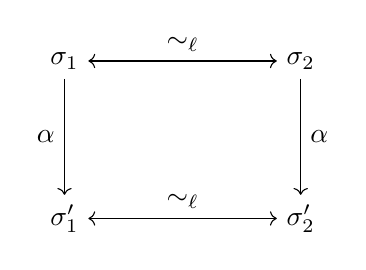
\begin{tikzpicture}
  \node (s1) at (0,2) {$\sigma_1$};
  \node (s2) at (3,2) {$\sigma_2$};
  \node (s1') at (0,0) {$\sigma'_1$};
  \node (s2') at (3,0) {$\sigma'_2$};
  
  \draw[<->] (s1) -- (s2) node[midway,above] {$\sim_\ell$};
  \draw[<->] (s1') -- (s2') node[midway,above] {$\sim_\ell$};
  
  \draw[->] (s1) -- (s1') node[midway,left] {$\alpha$};
  \draw[->] (s2) -- (s2') node[midway,right] {$\alpha$};
\end{tikzpicture}\]


    This property is also referred to as $\sigma_1$ and $\sigma_2$ being \textit{indistinguishable} with respect to public values.

This indistinguishability property is equivalent to requiring any map from some type $\tau_H$ to type $\tau_L$
to be constant. %\textit{weakly constant}. A function $f: X \to Y$ is weakly constant if for any $x_1,x_2 \in X$, $f(x_1) = f(x_2)$.
One characterization of this definition is the following:
\begin{proposition}
    For any closed function $\cdot \vdash f : \tau_H \to \tau_L$, there exists a closed $\cdot \vdash v : \tau_L$ such that $f \simeq \lambda\_.v$,
    meaning $f$ is observationally (extensionally) equivalent to a constant $v$ function.
\end{proposition}
\section{Categorical Background Potpourri}
In this section, we explain the medley of categorical concepts needed to understand Sterling and Harper's construction. %expand?
\subsection{Lattices and Logic}
\begin{definition}[Lattices]
\sloppy
    A lattice $\mathcal{L}$ is a partially ordered set which has all \textit{meets} and \textit{joins}.
    \begin{itemize}
        \item Two elements $l,k \in \mathcal{L}$ have a \textit{meet} if there exists an $m\in\mathcal{L}$
            such that $m$ is the greatest lower bound of $l$ and $k$. \textit{Joins} are symmetrically least upper bounds.
        \item Having all meets and joins means for any pair of elements in the lattice, you can find a greatest lower bound as well as a least upper bound. This property can also be phrased as having all binary products and all binary coproducts. 
    \end{itemize}
    A lattice with $\mathbf{0}$ and $\mathbf{1}$ (unique initial and terminal objects) has all finite limits and all finite colimits. 
\end{definition}
%People generally refer to a lattice of security levels $\ell$ when reasoning about information flow. The simplest example is the set $\{L,H\}$, where $L < H$, referring to low-security (public) and high-security (private) respectively.

Intuitionistic propositional logic can be thought of as a \textit{Heyting algebra }$H$, which is a lattice with $\mathbf{0}$ and $\mathbf{1}$, and has for each pair $x,y$ an exponential object $y^x$, usually written as $x \Rightarrow y$. Disjunction and conjunction are joins and meets, respectively, with the initial object $\mathbf{0}$ and terminal object $\mathbf{1}$ as their respective identities. That is,
\[ x \lor \mathbf{0} = x, \quad x \land \mathbf{1} = x\]

A \textit{distributive lattice} is a lattice in which 
\[x \land (y \lor z) = (x \land y) \lor (x \land z)\]
holds for all $x,y,z \in \calL$. This identity also implies the dual, $x \lor (y \land z) = (x \lor y) \land (x \lor z)$.

%We can also define negation, in terms of the notion of \textit{complement} for an element $x\in\calL$. In a distributive lattice, the complement is unique. If it exists, the unique complement of $x$, denoted $\neg x$, satisfies the following formulas:
% \[ x \lor \neg x = \mathbf{1}, \quad x \land \neg x = \mathbf{0}.\]

The exponential $x \Rightarrow y$ corresponds to implication. Writing out our usual diagram in the above language,
\[
\begin{tikzcd}[row sep=large, column sep=large]
z \land x \arrow[dr] \arrow[d] & \\
y^x \land x \arrow[r] & y
\end{tikzcd}
\]
we can characterize $y^x$ or $x \Rightarrow y$ by the following: 
\[z \land x \leq y \quad \iff \quad z \leq x \Rightarrow y\]
We can interpret $x \Rightarrow y$ as a least upper bound for $z$ such that $z \land x \leq y$. Negation in a Heyting algebra can be defined in the "implies absurdity" manner:
\[\neg x := x \Rightarrow \mathbf{0}\]
With our definition of $\Rightarrow$, this implies \[y \leq \neg x \quad \iff \quad y \land x = \mathbf{0},\]
where we have $=$ instead of $\leq$ because $\mathbf{0}$ is initial.

\marginnote{An alternative (cursed) answer to the question "what is a topology?" : a topology is \textit{just} something you define sheaves over, and sheaves are \textit{just} something you define a cohomology on, so the question you should really be asking is, what is a cohomology?}
\begin{definition}[Topology]
\sloppy
    A \textit{topology} on a set $X$ can be defined as a collection $\mathcal{T}$ of subsets of X, called \textbf{open sets} and 
    satisfying the following axioms:
    \begin{enumerate}
        \item The empty set and $X$ itself belong to $\mathcal{T}$.
        \item Any arbitrary union of members of $\mathcal{T}$ belongs to $\mathcal{T}$.
        \item The intersection of any finite number of members of $\mathcal{T}$ belong to $\mathcal{T}$.
    \end{enumerate}
\end{definition}
For a topological space $X$, the set of all open sets of $X$, notated $\calO(X)$, forms a Heyting algebra. This implies we can model the intuitionistic propositional calculus with any topological space $X$, by looking at the associated set $\calO(X)$. 
%potentially include Formula relation
\newpage
\begin{definition}[Special Subsets of Lattices]
\sloppy
    \begin{itemize}
        \item An \textit{upper set} U on a poset $(\calP,\leq)$ is upwards closed: if $x\in U$ and $x \leq z$, then $z \in U$. 
        \item Symmetrically, a \textit{lower set} U on $\mathcal{P}$ is downwards closed: if $x \in U$ and $z\leq x$, then $z\in U$.
        \item A \textit{filter} $\calF$ on $\calP$ is an upper set with the additional condition of every finite subset of $\calF$ having a lower bound in $\calF$ (filters are closed under finite meets)
    \end{itemize}
\end{definition}
\marginnote{For an example of an upper set which is \textit{not} a filter, consider the lattice of divisors of $12$ ordered by division. The upper set defined by $U = \{4,6,12\}$ is not a filter, since the meet (in this case gcd) of $4$ and $6$ is $2$, which is not contained in $U$. By contrast, $\{6,12\}$ satisfies filter requirements}
%\newpage
\begin{example}
Recalling that the natural numbers $\mathbb{N}$ form a poset ordered under divisibility, here is a Hasse diagram of the factors of $60$,
where the blue numbers are the elements of the upper set generated by $6$ (and in this case the upper set is also a filter), 
and the orange are elements of the lower set generated by $10$.

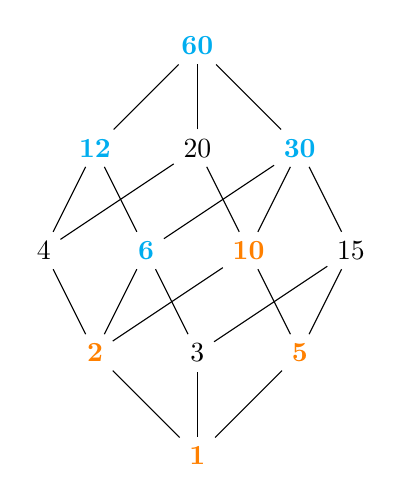
\begin{tikzpicture}[scale = 0.65]
  % Level 0: 1
  \node[orange] (1) at (0,0) {$\mathbf{1}$};
  
  % Level 1: prime divisors of 60
  \node[orange] (2) at (-2,2) {$\mathbf{2}$};
  \node (3) at (0,2) {$3$};
  \node[orange] (5) at (2,2) {$\mathbf{5}$};
  
  % Level 2: products of two primes
  \node (4) at (-3,4) {$4$};
  \node[cyan] (6) at (-1,4) {$\mathbf{6}$};
  \node[orange] (10) at (1,4) {$\mathbf{10}$};
  \node (15) at (3,4) {$15$};
  
  % Level 3: products of three primes
  \node[cyan] (12) at (-2,6) {$\mathbf{12}$};
  \node (20) at (0,6) {$20$};
  \node[cyan] (30) at (2,6) {$\mathbf{30}$};
  
  % Level 4: 60
  \node[cyan] (60) at (0,8) {$\mathbf{60}$};
  
  % Edges from 1
  \draw (1) -- (2);
  \draw (1) -- (3);
  \draw (1) -- (5);
  
  % Edges from 2
  \draw (2) -- (4);
  \draw (2) -- (6);
  \draw (2) -- (10);
  
  % Edges from 3
  \draw (3) -- (6);
  \draw (3) -- (15);
  
  % Edges from 5
  \draw (5) -- (10);
  \draw (5) -- (15);
  
  % Edges from 4
  \draw (4) -- (12);
  \draw (4) -- (20);
  
  % Edges from 6
  \draw (6) -- (12);
  \draw (6) -- (30);
  
  % Edges from 10
  \draw (10) -- (20);
  \draw (10) -- (30);
  
  % Edges from 15
  \draw (15) -- (30);
  
  % Edges from 12
  \draw (12) -- (60);
  
  % Edges from 20
  \draw (20) -- (60);
  
  % Edges from 30
  \draw (30) -- (60);
  
\end{tikzpicture} 
\end{example}
\begin{definition}[Alexandroff Topology]
\sloppy
    The \textit{Alexandroff Topology} is a natural topology on the underlying set of a pre-ordered set, where the open sets are the upper sets.
\end{definition}
\marginnote{(Foreshadowing): If we order filters $\calF$ on a poset $\calP$ by inclusion, we get a poset of the set of filters. This would imply there exists an Alexandroff topology to be defined here, with upper sets of the filters. }
Let's check that this definition satisfies the axioms for open sets.
\begin{proposition}
    Upper sets of a poset $\mathcal{P}$ satisfy the following axioms:
    \begin{enumerate}
        \item The empty set and $\mathcal{P}$ itself are upper sets.
        \item Upper sets are closed under arbitrary unions.
        \item Upper sets are closed under finite intersections.
    \end{enumerate}
\end{proposition}

 \begin{proof}.
    \newline
        \begin{enumerate}
            \item $\emptyset$ as an upper set is vacuously true; there are no elements to check. For $\mathcal{P}$,
        suppose $x \in \mathcal{P}$ and $x\leq y$. Well $y\in\mathcal{P}$ because $\mathcal{P}$ is the entire set.
            \item Let $\{U_i\}_{i \in I}$ be a collection of upper sets. We wish to show $\bigcup_{i \in I} U_i$ is an upper set.
            Suppose $x \in \bigcup_{i \in I} U_i$ and $x \leq y$. Then $x \in U_j$ for some $j \in I$. $U_j$ is an upper set
            and $x\leq y$, so $y \in U_j$. Then $y \in \bigcup_{i \in I}U_i$ so arbitrary union of upper sets is also an upper set.
            \item Let $U,V$ be upper sets. We want to show $U \cap V$ is an upper set. Suppose $x\in U \cap V$ and $x\leq y$.
            Then $x \in U$ and $x \in V$. Since $U$ and $V$ are both upper sets and $x\leq y$, we have $y \in U$ and $y \in V$. Then $y \in U\cap V$!
            So upper sets are also closed under finite intersection.  
        \end{enumerate}
\end{proof}


%\newpage
\subsection{Sheaves}

In the sheaf semantics chapter we defined a \textit{coverage}, which was defined to be a relation $T$ between families of morphisms with common codomain $c$ and objects $c$ of $\calC$. If a family $\{f_i: c_i \to c\}$ and object $c$ are in $T$, then $\{f_i : c_i \to c\}$ is a $T$-cover of $c$. Conditions for $T$ can be found in the aforementioned chapter. A general intuition for these families of morphisms is to think of them as a way to partition an object $c$ by images of $f_i$. 
\newpage
\begin{definition}[What is a sheaf, actually?]
%For this explainer, we refer to sheaves over topological spaces. Given a space $X$, a sheaf is a functor $\calO(X)^{op} \to$ \textbf{Set}, meaning sheaves act on the open sets of $X$. 

Let $\calC$ be a category with a coverage $T$. For any object $A \in \calC$, we have a T-cover $\{a_i : A_i \to A\}_{i \in I}$ indexed by some $I$. A presheaf $F$
on $\calC$ is a sheaf if it satisfies two additional conditions for \textit{any}\\T-cover:
\begin{enumerate}
    \item[1.] \textit{locality}: For any $f,g \in F(A)$, if $f\mid_{A_i} = g\mid_{A_i}$ for all $i \in I$, then $f = g$. The notation $f\mid_{A_i}$ is equivalent to applying $F(p_i)(f)$ \\where $p_i$ is the morphism $A_i \to A$.
    
    If two elements agree locally 
    (on each part of the cover), they \\agree everywhere. We can also think of this as being able\\ to partition any $f \in F(A)$ into the "sum of its parts", where 
    the \; parts correspond to an arbitrary cover of $A$. 
    \item[2.] \textit{gluing}: Let $f \in F(A)$. 
    For any $i,j \in I$, we have $F(\pi_i)(f\mid_{A_i}) = F(\pi_j)(f\mid_{A_j})$  in $F(A_i \times_A A_j)$, where $\pi_i$ is the projection\\ $A_i \times A_j \to A_i$, $\pi_j$ is the projection for $A_j$ and $A_i \times_A A_j$ is the pullback of $A$ along $f\mid_{A_i}$ and $f\mid_{A_j}$.  
    
    If $\calC$ is a preorder with meets, this simplifies to for any $x \in A_i \cap A_j$, we have $f\mid_{A_i} x = f\mid_{A_j} x$. 
    \begin{itemize}
        \item Consider the case where $F(A)$ maps to sets of functions. In \\this case, an equivalent definition to the above which may\\ have more of a "gluing" connotation says that, for any \\$f_i : A_i \to A$ and $f_j : A_j \to A$ such that $f_i(a) = f_j(a)$ for $a \in A_i \cap A_j$, there exists a unique $f$ such that $f\mid_i = f_i$ and $f\mid_j = f_j$. That is, when we have two maps agreeing at their intersection, we can "glue" them together to get another map.
    \end{itemize}
\end{enumerate}
\end{definition}

\begin{proposition}
\label{Proposition:eq->sheaf}
    Let $\calC$ be a category with a coverage and $F : \calC^{op} \to Set$. For any $A \in \calC$, for any cover $\{a_i : A_i \to A\}$ of $A$, $F$ is a sheaf iff $F$ satisfies 
    the equalizer diagram 
  \[F(A) \xlongrightarrow{e} \prod_{i \in I} F(A_i) 
    \begin{matrix}
    \xlongrightarrow{p} \\
    \xlongrightarrow{q}
    \end{matrix}
    \prod_{i,j \in I} F(A_i \cap A_j),\]
    where $p(f_i) = f_i \mid_{A_i \cap A_j}$ and $q(f_i) = f_j \mid_{A_i \cap A_j}$.
\end{proposition}

Brief sketch on why the above is true:
\begin{lemma}
\label{eqmonl}
    $e$ (or any equalizing map) is a monomorphism. Conversely, the morphism associated to the coequalizer is an epimorphism. These are not too hard to prove.

    Can see Solution \ref{eqmons}
\end{lemma}
\begin{itemize}
    \item Since $F$ maps to \textbf{Set}, $e$ is also injective. We can think of $e$ as the map that partitions some $f \in F(A)$,
    i.e. $e(f) = \{f\mid_{A_i}\}_{i \in I}$. Then agreeing locally, $f\mid_{A_i} = g\mid_{A_i}$, is equivalent to saying $e(f) = e(g)$. Injectivity of $e$ gives us
    $f = g$.
    \item The equalizer-ness of $F$ means $F(A)$ only consists of those $f$ where $p \circ e (f) = q \circ e (f).$ We are guaranteed 
    $\left( f \mid_{A_i} \right)\mid_{A_i \cap A_j} = \left( f \mid_{A_j} \right)\mid_{A_i \cap A_j}$, which is equivalent to saying $f\mid_{A_i} x = f\mid_{A_j} x$
    for all $x \in A_i \cap A_j$.
\end{itemize}

\begin{definition}[Topological Vocabulary]

    \begin{itemize}
        \item Let $U$ be an open subset of some $S$ with topology $\calT$. The family of open sets $C = \{U_i\}_{i \in i}$ indexed by some $I$ is an \textit{open cover} of $U$
    iff $\bigcup_{i \in I}U_i = U$.
        \item A family of open subsets $\{B_i\}_{i\in I}$ of $S$ form a \textit{basis} for $\calT$ iff for \\any $U\subset S$, there exists some $J \subset I$ such 
        that $\{B_i\}_{i \in J}$ is an open cover of $U$. That is, any element of $\calT$ (open set) can be \\represented as a union of some subset of the basis elements.
    \end{itemize}
\end{definition}
    For a space $S$, the topological definition of a covering corresponds to a coverage on $\calO(S)$, where the families of morphisms are inclusion maps. Recall $\calO(S)$ denotes the set of open sets of $S$, which form a poset (in fact, a heyting algebra) under inclusion. 

    Taking $C$ as an open cover of $U$ as above, we can write $C$ as \\$\{U_i \hookrightarrow U\}_{i \in I}$.

\begin{definition}[Subterminal Sheaf]
\sloppy
    Fix a category $\calC$
    \begin{itemize}
        \item Given a functor $F$, the functor $G$ is a \textit{subfunctor} of $F$ if $G(C)\subseteq F(C) \;\forall\; C\in\calC$. If $F$ is a sheaf on $\calC$,
        then $G$ is a \textit{subsheaf} if and only if for every open $U$ of $\calC$ and every element $f \in FU$, and every open covering $U = \bigcup U_i$, one has
        $f \in GU$ if and only if $f\mid_{U_i} \in GU_i$ for all $i$.
        \item The terminal sheaf is the terminal object $\mathbf{1}$ of $Sh(\calC)$. A \textit{subterminal sheaf} $F$ is a subsheaf of $\mathbf{1}$. $F$ is a subfunctor, meaning \newline $FC \subseteq \mathbf{1}C = 1$ for all $C\in \calC$. This means $FC$ can only be either $1$ or $\emptyset$.      
    \end{itemize}
\end{definition}
\begin{proposition}
    A \textit{subobject} of a sheaf $F$ in the category $Sh(\calC)$ is isomorphic to a subsheaf of $F$.
    \begin{proof}
        See \S II.3 in \textit{Sheaves in Geometry and Logic} by MacLane and Moerdijk.
    \end{proof}
    %\textcolor{red}{TODO}
\end{proposition}

\begin{theorem}
\label{Theorem:opens=sheaf}
    For any space $X$, there is an isomorphism \[\calO(X) \cong Sub_{Sh(X)}(\mathbf{1})\] of partially ordered sets.

    \begin{proof}$\Rightarrow$

        Given any open set $W$ of $X$, define a functor $S_W$ on open sets $U$ by $S_W(U) = 1$ if $U\subseteq W$ and $\emptyset$ otherwise. Recall $\mathbf{1}U = 1$ for all open $U$. Let $\{V_i\}$ be an arbitrary covering of $U$. If $S_W(V_i) = 1$ for all $i$, then $\bigcup V_i \subseteq W$, meaning $U \subseteq W$, so $S_W(U) = 1$. In the other direction, if $S_W(U) = 1$, all $V_i \subseteq U$ so $S_W(V_i) = 1$ for all $i$. So, we can see $S_W$ is a subsheaf of $\mathbf{1}$.
        
        $\Leftarrow$

        Let $S$ be a subsheaf of $\mathbf{1}$. Each $S(U)$ must then be either $1$ or $\emptyset$. If $S(U) = 1$ and $V \subseteq U$, and $S$ requires a morphism $S(U) \to S(V)$ meaning $1 \to S(V)$, it follows that $S(V)$ is nonempty and thus $S(V) = 1$. By the equalizer condition, if $\{V_i\}$ is an open cover of $U$ and $SU_i = 1$ for all $i$, then $SU = 1$. 

        Define $W = \bigcup\{U \in \calO(X) | SU = 1\}$. Then by equalizer condition we have $SU = 1$ if and only if $U \subseteq W$. Then we have $S = S_W$, so we have the bijection $W \iff S_W$.
    \end{proof}

\end{theorem}

\subsection{Special Sheaf Functors}
\label{ssf}
The crux of the Sterling and Harper's information flow model is based on the following monad definition:

"For any subspace $Q\subset P$, a sheaf $A \in Sh(P)$ can be restricted to $Q$, as in $A\mid_Q \in Sh(Q)$, and then extended again to $P$. This composite defines an \textit{idempotent} monad on $Sh(P)$ that we can interpret as removing any data from $P$ that cannot be seen from $Q$."

\marginnote{A monad $T$ is idempotent when $T^2 = T$ (i.e. $\mu = $iso).}

This construction is a specialization of a much more general property of sheaves, which we need to do some work to define.

\begin{definition}
    Let $X,Y$ be topological spaces. A function $f : X \to Y$ is \textit{continuous} if, for every open $V \subseteq Y$, the preimage $f^{-1}(V)$ is open in $X$.
\end{definition}
\begin{exercise}
\label{ex1e}
    All monotone maps in the Alexandroff topology are continuous.

    See Solution \ref{ex1s}
\end{exercise}

%A \textit{bundle} over an object $B$ is an object $E$ equipped with a morphism $E \xrightarrow{p} B$. All bundles over $B$ form a category: the slice category $\calC / B$.

\begin{definition}[Direct Image Sheaf Functor]
    
    Given a continuous $f$, each sheaf $F$ on $X$ yields a sheaf $f_*F$ on $Y$ \\defined for $V$ open in $Y$, by $(f_*F)V = F(f^{-1}V)$. Essentially, $f_*F$ is the composite functor 
   \[\calO(Y)^{op}\xlongrightarrow{f^{-1}}\calO(X)^{op}\xlongrightarrow{F}\textbf{Set}\]
   This sheaf is called the \textit{direct image} of $F$ under $f$. The map \\
   $f_*:Sh(X) \to Sh(Y)$ is a functor of sheaf categories.

\end{definition}
%\begin{remark}
   \marginnote{In the measure theory/qbs lecture, we briefly discussed the pushforward of a measure along a measurable map: $\mu_B(b) = \mu_A(f^{-1}(b))$ where $f^{-1}$ is the preimage. We can similarly think of $\mu_B$ as the composite functor $\Sigma_B \xrightarrow{f^{-1}} \Sigma_A \xrightarrow{\mu_A} [0,1]$, where we might want to denote $\mu_B$ by $f_*\mu_A$, and say $f_*$ is a functor of probability measures.}
%\end{remark}

A continuous $f: X \to Y$ also induces a functor $f^*:Sh(Y) \to Sh(X)$, where each sheaf $G$ on $Y$ yields a sheaf $f^*G$ on $X$. We typically can't define $f^*$ (the Inverse Image Functor) as simply as we were able to define $f_*$ because we don't know if $f(U)$ is open (continuity only gives us information about preimages). 

First we have the general and scary definition (though not the most general because we assume sheaves over topological spaces):
\begin{definition}[Inverse Image Sheaf Functor]
\label{Definition:invsheaf}
    Let $f:X \to Y$ be a continuous map of topological spaces. For any sheaf $G$ on $Y$, we define the \textit{inverse image} sheaf $f^*G$ on $X$ to be the \textit{sheafification} of the presheaf $U \mapsto \colim_{V \supseteq f(U)}G(U)$, where $U$ is any open set in $X$, and the limit is taken over all open sets $V$ of $Y$ containing $f(U)$. 
\end{definition}
Luckily for us, the only continuous maps we care about in this chapter are inclusion maps. Here is some sketchy / informal reasoning as to why $i^*F(U) = F(U)$ when $X \subseteq Y$ is open for open $U \subseteq X$.
\begin{itemize}
    \item When $X \subseteq Y$ is open any open $U \subseteq X$ is open in $Y$ as well.
    \item $F(U)$ would be the colimit of $F(V)$ where $V \supseteq i(U) = U$, because $U$ is clearly the greatest lower bound (limit) on sets containing $U$, so dually $F(U)$ would be the least upper bound (colimit) on $F(V)$ with $V \supseteq U$, since $F$ is contravariant.
    \item Then $i^*F(U) = F(U)$, and of course $F$ is a sheaf so $i^*F(U)$ automatically satisfies sheaf conditions for open $U$. 
\end{itemize} 

If $X$ is not open, we have a more complicated situation, where open $U \subseteq X$ is not guaranteed to be open in $Y$. 

If we are working in a topology $\calT$ where for every (not necessarily open) subset $V$ of a space $Y$ has a smallest open $U \subseteq Y$ such that $V \subseteq U$, then $i^*F(V) = F(U)$. Let's notate this smallest open $U$ for $V$ by $o(V)$. To have $i^*F$ satisfy sheaf conditions, we need covers to "behave well", that is, for $\bigcup_j V_j = V$, we need $\bigcup_j o(V_j) = o(V)$. In general this is not guaranteed. 

However, in this chapter we will only be looking at the Alexandroff topology. In this topology the open sets are upper sets, so for any set $V$, we have $o(V) =\uparrow V$, where $\uparrow V$ represents the upwards closure of $V$, basically turning $V$ into an upper set. The upwards closure $\uparrow$ respects/distributes across unions, that is $\bigcup_j \uparrow V_j = \uparrow \bigcup_j V_j$. So we do not need to worry about sheafifying anything!


%Luckily, for the purposes of this chapter, we only care about inclusion maps, which are \textit{open maps}, meaning the images of open subsets \textit{are} open! 

%\begin{definition}[Étale Spaces]
%    Let Top be a category of topological spaces
%    \begin{itemize}
%        \item A \textit{homeomorphism} is an isomorphism in Top (isomorphism of \quad \quad \; topological spaces)
%        \item Let $B$ be an object in Top. An \textit{etale space} over $B$ is a bundle \quad\quad\quad\;     
%        $p : E \to B$, such that for every $e \in E$, there exists an open subset $U$ containing $e$ such that $p(U)$ is open in $B$ and the restriction $p\mid_U: U \to p(U)$ is a homeomorphism.
%    \end{itemize}
%\end{definition}

%Essentially, étale spaces are defined precisely to give us information about openness in the image of a continuous map. For the purposes of this chapter, don't worry too much about them beyond that. 

%Let $f: X \to Y$ continuous in category $\calC$. Each étale bundle $p: E \to Y$, pulled back along $f$, yields a bundle $f^*E \to X$ over x, and $f^*$ is a functor $f^* : \textbf{Etale } Y \to \textbf{Etale } X$.  
%\[
%\begin{tikzcd}[row sep=large, column sep=large]
%f^*E \arrow[r] \arrow[d] & E \arrow[d, "p"] \\
%X \arrow[r, "f"'] & Y
%\end{tikzcd}
%\]

%We have an equivalence of categories $Sh(-) \cong \textbf{Etale }(-),$ with $\Lambda : Sh(-) \to \textbf{Etale }(-)$ and $\Gamma : \textbf{Etale }(-) \to Sh(-)$.


\begin{theorem}
    \label{Theorem:adjoint-sheaves}
If $f : X \to Y$ is a continuous map, then the functor $f^*$, sending each sheaf $G$ on $Y$ to its inverse image (preimage) on $X$, is left adjoint to the direct image functor $f_*$ : 
\[
\begin{tikzcd}
Sh(X) \arrow[r, shift left, "f_*"] & 
Sh(Y) \arrow[l, shift left, "f^*"]
\end{tikzcd}, \quad f^* \dashv f_*
\]
\begin{proof}
    See \S II.9 in \textit{Sheaves in Geometry and Logic} by MacLane and Moerdijk.
\end{proof}
\end{theorem}

\cref{Theorem:adjoint-sheaves} is included to note that $f_* \circ f^*$ is a monad on $Sh(Y)$. Particularly, when $X \subset Y$ and $f$ is the inclusion map $i$, we have a monad given by $i_* \circ i^*$. It is precisely this composition which defines Sterling et al.'s idempotent monad.

The preimage of the inclusion map $i : Q \hookrightarrow P$ is defined $i^{-1}(V) = V \cap Q$, where $V$ is an open subset of $P$. With this, let's compute this monad for any inclusion. Fix a sheaf $F$ and $V$ open in $P$.
\begin{align*}
    i_* (i^* F)(V) &= (i^* F)(i^{-1} V)\\
    &= (i^* F)(V \cap Q)
\end{align*}

Recall that in our special case, the functor $i^*$ operates by $i^*F(U) = F(\uparrow U)$ for open $U$ in subspace $Q$, where $\uparrow U$ is the upward closure of $U$ in $P$. When $Q$ is open in $P$, $i^*F(U) = F(U)$. 

For any sheaf $F$, $F(\emptyset) = 1$. We can see this from the equalizer definition, where $F$ in this case is the equalizer of the empty diagram, which is precisely the terminal object.

If $V \cap Q \neq \emptyset$, then $i_*(i^* F)(V) = F(\uparrow (V \cap Q))$. If $V\cap Q = \emptyset$, then $i_*(i^* F)(V) = 1$.

\subsection{Pushouts} 
Let $X$ be a topological space and $Y$ an open set in $X$. One of the monads that Sterling et al. define is the composition of $i_* \circ i ^*$ defined by $i : X\setminus Y \hookrightarrow X$. The authors mention that this monad $i_* \circ i^*$ can be identified with a pushout construction \[Y \sqcup_{Y \times (-)} (-): Sh(X) \to Sh(X),\] where $Y$ here is treated as the subterminal sheaf where $Y(U) = 1$ if $U \subseteq Y$, and $\emptyset$ otherwise. This construction is key for later noninterference proofs, so we provide some intuition for how pushouts work/behave.


Pushouts are dual to pullbacks, but it is not very intuitive to get a sense of what that means exactly. We can try to work it out by staring at the diagram in \textbf{Set}:

\[
\begin{tikzcd}[row sep=large, column sep=large]
A \arrow[r, "f"] \arrow[d, "g"'] & B \arrow[d, dashed, "i_B"] \arrow[ddr, bend left, "h"] & \\
C \arrow[r, dashed, "i_C"'] \arrow[drr, bend right, "k"'] & P \arrow[dr, dashed, "\exists! u"] & \\
& & X
\end{tikzcd}
\]

Where $P$ is the smallest object with morphisms $i_C, i_B$, such that $i_C\circ g = i_B\circ f$, i.e. $i_C(g(a)) = i_B(f(a))$ for all $a \in A$. Then we can see that this restriction is only for the images of $f$ and $g$; we don't have any equality condition on $b \notin im(f), c\notin im(g)$.  
These maps $i_B, i_C$ are canonically \textit{quotient maps} modulo the relation by $f$ and $g$, meaning they map $b \in B, c \in C$ to equivalence classes $[b],[c] \in P$, with this extra equivalence condition. 

So, we can interpret the commutativity of this square to mean that for $b,c$ where there exists an $a$ such that $f(a) = b, g(a) = c$, we require $i_B(b) = [b] = [c] = i_C(c)$.

In \textbf{Set}, $P$ is a "quotient of the disjoint union of $A$ and $B$", which can also be written $A\sqcup B/\sim$, where $\sim$ is the equivalence relation generated by the restriction detailed above, i.e. some $\sim$ satisfying $b \sim c$ when $\exists\; a\in A$ such that $f(a) = b, g(a) = c$. The pushout essentially collapses the images of $f$ and $g$ to equivalence classes in $P$. We provide a couple of examples in \textbf{Set}. 

\begin{example}[pushout of product]
    Let $B,C$ be nonempty sets.
\[
\begin{tikzcd}[row sep=large, column sep=large]
B \times C \arrow[r, "\pi_1"] \arrow[d, "\pi_2"'] & B \arrow[d, "i_B"] \\
C \arrow[r, "i_C"'] & B \sqcup_{B \times C} C \arrow[ul, phantom, very near start]
\end{tikzcd} \cong 
\begin{tikzcd}[row sep=large, column sep=large]
B \times C \arrow[r, "\pi_1"] \arrow[d, "\pi_2"'] & B \arrow[d, "i_B"] \\
C \arrow[r, "i_C"'] & \{*\} \arrow[ul, phantom, very near start]
\end{tikzcd}
\]
By definition of product, for every $b\in B$ and for every $c\in C$, there exists an $a \in A$, namely $(b,c)$, such that $\pi_1((b,c)) = b$ and $\pi_2((b,c)) = c$. Then every element of $B$ is in the same equivalence class as every element of $C$, and by transitivity of equality, every element of $B$ is in the same equivalence class, as well as every element of $C$. Then $P$ only has one equivalence class, so $P$ is a singleton set and thus isomorphic to the terminal object.

\end{example}
\begin{example}[pushout of the initial object, 0]
    Recall that if a category has a terminal object and pullbacks, then it has products. This is the dual for "initial and pushout imply coproducts".
    \[
\begin{tikzcd}[row sep=large, column sep=large]
0 \arrow[r, "!"] \arrow[d, "!"'] & B \arrow[d, "i_B"] \\
C \arrow[r, "i_C"'] & B \sqcup_{0} C \arrow[ul, phantom, very near start]
\end{tikzcd} \cong 
\begin{tikzcd}[row sep=large, column sep=large]
0 \arrow[r, "!"] \arrow[d, "!"'] & B \arrow[d, "i_B"] \\
C \arrow[r, "i_C"'] & B \sqcup C \arrow[ul, phantom, very near start]
\end{tikzcd}
\]
The empty set is the initial object in \textbf{Set}. There are no $b,c$ such that $f(a) = b, g(a) = c$ because there are no $a \in A \cong \emptyset$. Then each $b$ and $c$ are distinct, resulting in the disjoint union of $B$ and $C$. 

Going back to our product example, suppose $B$ is empty and $C$ is nonempty. The product $B \times C$ is isomorphic to $0$, so we would get $B\sqcup C = \emptyset\sqcup C = C$. If $B$ and $C$ are empty, then naturally the pushout would be empty as well.

\end{example}
Let's look at how pushouts behave with presheaves. Let $F,G \in [C^{op};Set]$.
\begin{example}[pushout of $F\times G$]
\label{Example:fxg}
    This example is interesting because it does not automatically collapse to $\{*\}$.
    Functors are defined by how they act on objects, so for some $A \in \calC$ we have 
    \[
    \begin{tikzcd}[row sep=large, column sep=large]
    (F \times G)(A) \arrow[r, "\pi_{1A}"] \arrow[d, "\pi_{2A}"'] & F(A) \arrow[d, dashed, "i_B"] \\
    G(A) \arrow[r, dashed, "i_C"'] & F(A) \sqcup_{(F\times G)(A)} G(A) \arrow[ul, phantom, very near start]
    \end{tikzcd} 
\]
Where the projection maps are now natural transformations, also defined component-wise. Recall $(F \times G)(A)\cong F(A)\times G(A)$. We end up with 3 (really 4) cases for the pushout:
\begin{enumerate}
    \item F(A) and G(A) are nonempty. Then we have the typical product - pushout, so in this case we do get $1$ or $\{*\}$.
    \item F(A) is nonempty and G(A) is empty. Then $F(A)\times G(A) = \emptyset$. Pushout from the initial object gives us $F(A) \sqcup G(A) = F(A) \sqcup \emptyset = F(A)$. We have a symmetric case for F(A) empty and G(A) nonempty.
    \item F(A) and G(A) are empty. This yields $\emptyset \sqcup \emptyset = \emptyset$
\end{enumerate}
Sheaves are a little more complicated. If we compute a pushout of a product of sheaves $S,P$ as above, we can define the result point-wise as a presheaf, but we are not guaranteed that this presheaf satisfies the sheaf conditions. \marginnote{The general solution to this is to \textit{sheafify} the computed presheaf pushout, which is currently out of the scope of this chapter.}
\end{example}

\newpage


%Fix a poset (partially ordered set) $\mathcal{P}$ of security levels closed under finite meets. For the remainder of this chapter we assume \[\mathcal{P} := \{L \subset M \subset H \subset \top\}.\]

%Sterling uses an Alexandroff topology, which is a structure of a topological space induced on the underlying set
%of a preordered set. 

\section{Sheaf Semantics for Noninterference (putting it all together)}
We are now ready to talk about some of the central ideas of the paper. This section will culminate in a proof of a form of noninterference where sheaves are interpreted as types. 

Fix a poset $\mathcal{P}$ of security levels closed under finite meets.

\begin{definition}
    \begin{itemize}
        \item An \textit{abstract behavior} $x$ is a filter on the poset $\mathcal{P}$. We can interpret this as saying $x$ denotes the security levels where a behavior is permitted.
        \begin{itemize}
            \item For example, a filter generated by M would include H and $\top$, capturing that medium-security information/behavior can be used at higher-security levels.
        \end{itemize}
        \item A \textit{security policy} U is a lower set in $\mathcal{P}$. The notation $U \vdash x$ is \\pronounced "U permits $x$", and means $U \cap x \neq \emptyset$. 
        \begin{itemize}
            \item Consider the poset $\{L \leq M \leq H\}$. Supposing we have a security policy generated by M: this includes L and M, and can be understood as denoting the security levels \textit{above} which \\some information/behavior is permitted. Alternatively, 
        the \\set where this behavior is not allowed.
        \end{itemize}
    \end{itemize}
\end{definition}
\begin{definition}
    The authors define $P$ to be the topological space where points are abstract behaviors, and the open sets are of the form $\{x \mid U \vdash x\}$.
\end{definition}

%\begin{proposition}
    %This space is the Alexandroff topology on the space of filters of $\calP$. 
    %\begin{proof}
        %The set of filters on $\calP$, ordered by inclusion, forms a poset. Once we show the sets $O_U := \{x \mid U \vdash x\}$ are upper sets of the filters, we are done.
        
        %Fix some lower set $U$ of $\calP$ and suppose $x \in O_U$. Let $y \in P$ such that $x \subseteq y$. Then $x \cap U \neq \emptyset$ immediately implies $y \cap U \neq \emptyset$ because $x \cap U \subseteq y \cap U$. 

        %Now, let $V$ be an upper set on Filters$(P)$ and suppose $x \in V$. 
   % \end{proof}
%\end{proposition}
%newpage
\begin{exercise}
    \label{ex2e}
    Prove these sets are open with the openness axioms.

    See Solution \ref{ex2s}
\end{exercise}


Each security level $\ell \in \mathcal{P}$ represents a security policy $\angled{\ell}$ of the form $\{a \in \calP \mid a \leq \ell\}$. The 
corresponding open subspace of $P$, $(\{x \mid \angled{\ell} \vdash x\})$ is denoted $P_{\angled{\ell}}$. The complement, $P \setminus P_{\angled{\ell}}$ is denoted $P_{\bullet \angled{\ell}}$.
\newpage
\begin{proposition}
\label{Proposition:ell-in-x}
    The predicate $\angled{\ell} \cap x \neq \emptyset$ is equivalent to $\ell \in x$. 
\end{proposition}
To see the above, suppose we have some nonempty intersection for $\angled{\ell}$ and $x$. Then there exists some $k \in \angled{\ell}$ such that $k \in x$.
Since $k \in \angled{\ell}$, this means $k \leq \ell$. Since $x$ is a filter and hence upwards closed, since $\ell \geq k$ and $k \in x$, we have $\ell \in x$. 
The other direction is immediate since $\ell \in \angled{\ell}$ so $\ell \in x$ clearly implies a nonempty intersection. 
%This construction is an Alexandroff topology on the space of filters on $\mathcal{P}$ --- the space where the points/elements are abstract behaviors.

\begin{proposition}
    Let $\angled{\ell_1}$ and $\angled{\ell_2}$ be security policies such that $\ell_1 < \ell_2$. Then
    $P_{\angled{\ell_1}} \subset P_{\angled{\ell_2}}$.
    \begin{proof}
        Let $x$ be an abstract behavior in $P_{\angled{\ell_1}}$, i.e. a filter on $\mathcal{P}$ such that ${\angled{\ell_1}} \cap x \neq \emptyset$.
        Then there is some $y$ in this intersection, meaning $y \in x$ and $y \leq \ell_1$. Since $\ell_1 < \ell_2$ and posets have transitivity,
        $y < \ell_2$, which means $y \in \angled{\ell_2}$. Then $y \in x \cap \angled{\ell_2}$, so $x \in P_{\angled{\ell_2}}$.
    \end{proof}
\end{proposition}

\subsection{Sheaf Interpretation}

In this subsection, we parse Sterling et al.'s statement: \textit{"our intention is to interpret each type of a dependency core calculus as a sheaf on the space $P$ of abstract behaviors. to see why this interpretation is plausible as a basis for secure information flow, we note that a sheaf on $P$ is the same thing as a presheaf on the poset $\mathcal{P}$"}. 

\begin{itemize}
    \item In this context, the only relevance of dependency core calculus is that it is a typed programming language where types can be annotated with security levels from some poset.
    \item This statement assumes a presheaf interpretation over $\calP$ is understood to be a plausible basis for modeling information flow, so let's justify this quickly:
    \begin{itemize}
        \item Consider the presheaf category over $\mathcal{P}$. This has a natural representation for information flow : for each security level $\ell$, we have a set $F(\ell)$ representing what data is visible under security level $\ell$. Since presheaves are contravariant functors, for each $k \leq l$ in $\calP$, we get a morphism $F(\ell) \to F(k)$, demonstrating the restriction of information to that at a lower security level.        
    \end{itemize}
    \item Now we have this note : a sheaf on $P$ is "the same thing" as a presheaf on the poset $\mathcal{P}$. This sounds like a bijection.
\end{itemize}


\begin{theorem}
\label{Theorem:P=S}
There is a bijection between the presheaf category $Psh(\calP)$ and the sheaf category $Sh(P)$.
\end{theorem}

Recall the topological space at hand, $P$, has open sets of the form $\{x \mid U \vdash x\}$, where $U$ is a lower set, $x$ is a filter, and 
$U \vdash x$ means $U \cap x \neq \emptyset$. Note that the open sets are defined by the lower sets of $\cal P$, so we will denote them by $O_U,$ where $U$ 
is the lower set of choice. Now we have a series of lemmas.

\begin{lemma}
    The family $\{P_{\angled{\ell}}\}_{\ell \in \calP}$ is a basis for the topology on $P$. 
    \begin{proof}
    %i think i almost have to tbh its so far apart at this point
    We know each $P_{\angled{\ell}} = \{x \mid \angled{\ell} \vdash x\}$ are open by definition. 

    Let $U$ be an upper set of $\calP$ and $O_U$ the corresponding open set of $P$, so 
    $O_U = \{x \mid x \cap U \neq \emptyset\} = \{x \mid \exists\; \ell\in U : \ell \in x\}$. We can tranform this into 
    \[\bigcup_{\ell \in U}\{x | \ell \in x\} = \bigcup_{\ell \in U}\{x \mid \angled{\ell} \vdash x\} = O_U,\]
    where the second expression comes from \cref{Proposition:ell-in-x}. So, we have a family of nonempty open sets of the form $P_{\angled{\ell}}$ indexed by some subset of 
    $\calP$ (as some of the sets in the above union will be naturally empty) such that their union is equal to $O_U$ in $P$. 
    \end{proof}
\end{lemma}
\begin{lemma}
    Let $\ell, k \in \calP$. We claim $P_{\angled{\ell}} \cap P_{\angled{k}} = P_{\angled{\ell \land k}}$
    \begin{proof}
        Note we have $\ell \land k$ for any $\ell,k \in \calP$ because $\calP$ is closed under finite meets. Suppose we have some $x \in P_{\angled{l\land k}}$,
        meaning $\ell \land k \in x$. Since $x$ is upwards closed and $\ell \land k$ is the meet of $\ell$ and $k$, it follows immediately that $\ell \in x$ and $k \in x$,
        meaning $x \in P_{\angled{\ell}} \cap P_{\angled{k}}$. 

        For the other direction, we begin with $\ell \in x$ and $k \in x$. Since $x$ is a filter, any finite subset of $x$ has a lower bound in $x$. Considering $\{\ell,k\}$
        as our subset, suppose we have some lower bound $q \in x$. By definition of meets, $q \leq \ell \land k$, so $\ell \land k \in x$,
        meaning $x \in P_{\angled{\ell \land k}}$. This reasoning also tells
        us that filters on a poset are closed under finite meets.
    \end{proof}
\end{lemma} 
\marginnote{There is an alternate (perhaps more elegant) theorem in MacLane and Moerdijk demonstrating the same property as \cref{lemma:basis}: Let $\calB$ be a basis for a topology on a space $X$. The restriction functor $Sh(X) \to Sh(\calB)$ is an equivalence of categories. They leave the proof as an exercise for the reader.}
\begin{lemma}\label{lemma:basis}
Any sheaf on $P$ is determined by values on the basis $\{P_{\angled{\ell}}\}_{\ell \in \calP}$.
\begin{proof}
    Fix some sheaf $F$ on $P$ and let $O_U$ be open in $P$. There exists some subset $\calQ \subset \calP$ 
    such that $O_U = \bigcup_{\ell \in \calQ}P_{\angled{\ell}}$, so $\{P_{\angled{\ell}}\}_{\ell \in \calQ}$ is a covering of $U$. Since $F$ is a 
    sheaf, it must satisfy
    \[F(O_U) \xlongrightarrow{e} \prod_{\ell \in \calQ} F(P_{\angled{\ell}}) 
    \begin{matrix}
    \xlongrightarrow{p} \\
    \xlongrightarrow{q}
    \end{matrix}
    \prod_{\ell,k \in \calQ} F(P_{\angled{\ell}} \cap P_{\angled{k}}),\]
    which is equal to 
    \[F(O_U) \xlongrightarrow{e} \prod_{\ell \in \calQ} F(P_{\angled{\ell}}) 
    \begin{matrix}
    \xlongrightarrow{p} \\
    \xlongrightarrow{q}
    \end{matrix}
    \prod_{\ell,k \in \calQ} F(P_{\angled{\ell \land k}}).\]
    %Let $s \in F(O_U)$, so $s$ can be written as a family $\{s_\ell\}_{\ell \in \calQ}$ such that $s_\ell \in F(P_{\angled{\ell}})$ for each $\ell \in \calQ$.
    Then to compute behavior of $F$ on $O_U$ such that the sheaf conditions are satisfied, we only need to know how $F$ acts on the basis, since we have rewritten 
    the rest of the diagram in terms of the basis elements.
\end{proof}
\end{lemma}  

Okay, now we are ready to prove \cref{Theorem:P=S}!
\begin{proof}.\newline
    \begin{enumerate}
        \item $Psh(\calP) \to Sh(P)$:  
        \marginnote{We could also be done after this definition, since we have a unique definition of $F$ on the basis, and the fancier theorem says $F(\calB)$ is equivalent to $F(P)$, where $\calB$ is a basis for $P$.}
        Let $E$ be a presheaf on $\calP$. We will use $E$ to define a sheaf $F$ on $P$. We have the natural behavior
        for the basis elements: $F(P_{\angled{\ell}}) := E(\ell)$. 

        As we showed above, all the other open sets follow immediately when we set $F(O_U)$ as the equalizer of the diagram with the covering of choice being the 
        basis elements. Note that this extends to arbitrary coverings, as each open set can be written itself as a union of basis elements, so no matter what we can
        always reduce a covering to its basis elements. 
        
        F maintains all the presheaf requirements as well: suppose $P_{\angled{\ell}} \subset P_{\angled{k}}$. We've shown this implies $\ell \leq k$. 
        Then we have a restriction morphism $E(k) \to E(\ell)$, and by definition this yields a restriction morphism 
        $F(P_{\angled{k}}) \to F(P_{\angled{\ell}})$. Defining $F(O_U)$ to be the equalizer of the given diagram gives us the desired sheaf conditions, as 
        sketched in \cref{Proposition:eq->sheaf}.
        \item $Sh(P) \to Psh(\calP)$:
        Set $E(\ell)$ to $F(P_\ell)$ for all $\ell \in \calP$. 
        
    \end{enumerate}
    
\end{proof}

\newpage

\subsection{Transparency and Sealing Monads}
These transparency and sealing monads are precisely instances of $i_* \circ i^*$, as defined in \cref{ssf}.
\begin{definition}

\label{Definition:t+smonads}
    \begin{enumerate}
        \item[1.] The \textit{transparency monad} $\angled{\ell} \Rightarrow A$ replaces $A$ with whatever part of it can be viewed under policy $\angled{\ell}$. If we define $i:P_{\langle \ell \rangle} \hookrightarrow P,$ the composition $i_* \circ i^*$ defines the unit $\eta_\Rightarrow:Sh(P) \to Sh(P)$ where $A \mapsto (\angled{\ell}\Rightarrow A)$. When the unit is an isomorphism at $A$, we say that $A$ is \textit{$\angled{\ell}$-transparent}.
        
        \item[2.] The \textit{sealing monad} $\angled{\ell} \bullet A$ removes from $A$ whatever part of it can be viewed under policy $\angled{\ell}$. If we define $i:P\setminus P_{\langle \ell \rangle} \hookrightarrow P,$ the composition $i_* \circ i^*$ defines the unit $\eta_\bullet:Sh(P) \to Sh(P)$ where $A \mapsto (\angled{\ell}\bullet A)$.
        \begin{itemize}
            \item The sealing monad can be constructed as the pushout \\ $P_{\angled{\ell}} \sqcup_{P_{\angled{\ell}} \times A} A.$ When the unit is an isomorphism at $A$, we say $A$ is \textit{$\angled{\ell}$-sealed}.
        \end{itemize}
    \end{enumerate}
\end{definition}
\begin{proposition}
\label{Theorem:tfunc}
    Sterling et al. claim the transparency monad "is" the function space $A^{P_{\angled{\ell}}}$, i.e. $A^{P_{\angled{\ell}}} \cong \angled{\ell} \Rightarrow A$. We will sketch a proof for the general case of open $Y$ in $P$.
    \marginnote{You may notice we are treating the open space $P_{\angled{\ell}}$ (and general $Y$) as a sheaf. Recall \cref{Theorem:opens=sheaf}, which proves Sterling et al.'s statement that an open set of $P$ is "the same" as a subterminal sheaf.}
    \begin{proof}(sketch)

        Let $j: Y \hookrightarrow P$ and $A$ be a sheaf on $P$. We want $j_*j^* A \cong A^Y$. One definition of the exponential object on sheaves over $\calO(X)$ is 
        \[A^Y(U) \cong \Hom(Y\mid_U,A\mid_U)\]
        where $Y\mid_U,A\mid_U$ are the sheaves restricted to subsets of $U$. Since $Y\mid_U(V) = 1$ if $V \subseteq U \cap Y$ and $\emptyset$ otherwise, any morphisms (natural transformations) $Y\mid_U \to A\mid_U$ are characterized by $V\subseteq U \cap Y$.  
    
        Let $\alpha$ be a natural transformation and $\alpha_V$ the component associated to $V \subseteq U \cap Y$, i.e. $\alpha_V : Y\mid_U(V) \to A\mid_U(V) = A(V)$. This simplifies to
        $\alpha_V : 1 \to A(V)$. There is a natural isomorphisms between $\Hom(1,A)$ and $A$, for any object $A$, so $\alpha_V$ is naturally isomorphic to $A(V)$. The subsets $V$ form a cover of $U\cap Y$, so we should be able to glue the nontrivial components of $\alpha$ (i.e., $\alpha\mid_{U \cap Y}$) to get $A(U\cap Y)$. Then we have 
        \begin{align*}
            \Hom(Y\mid_U,A\mid_U) &\cong \Hom(Y\mid_{U\cap Y},A\mid_{U\cap Y})\\
            &\cong \{A(V)\mid V \subseteq U \cap Y\}\\
            &\cong A(U \cap Y)
        \end{align*}
        In \cref{ssf}, we demonstrated $j_*j^*A(U) = A(U\cap Y)$ for $j : Y \hookrightarrow P$, so we have $j_*j^*A \cong A^Y$.
    \end{proof}
\end{proposition}



Given space $P$ and arbitrary $\angled{\ell} \in P$, the subspace defining the transparency monad $\angled{\ell}\Rightarrow$ is $P_{\angled{\ell}}$, and the subspace defining the sealing monad $\angled{\ell}\bullet$ is $P_{\bullet \angled{\ell}}$. 

Closed sets are defined to be complements of open sets. It is rare that the complement of an open set will also be open (called clopen sets). Note that $P_{\bullet \angled{\ell}}$ is not guaranteed to be open -- this is where the caveats of \cref{Definition:invsheaf} with respect to the Alexandroff topology come in. That is, for every open $U \in P_{\bullet \angled{\ell}}$, we have $i^*F(U) = F(\uparrow U)$ where $\uparrow U$ is the upward closure of $U$ in P. 
%The sealing monad has a weirder form that is hard to capture accurately with the inclusion adjunction, so we will think of it primarily by the pushout definition.
%\textcolor{red}{tbd. talk to john}
\begin{example}
Let's fix $\calP := \{L \subset M \subset H \subset \top\}$.

    There are only four filters on $\calP$, so we can write all of them out:
    \begin{align*}
        p_0 &= \{L, M, H, \top\} \\
        p_1 &= \{M, H, \top\} \\ 
        p_2 &= \{H, \top\}\\
        p_3 &= \{\top\}
    \end{align*}
    From here, we can also enumerate the principal open sets on $P$:
    \begin{align*}
        P_{\angled{L}} &= \{p_0\}\\
        P_{\angled{M}} &= \{p_0, p_1\}\\
        P_{\angled{H}} &= \{p_0, p_1\, p_2\}\\
        P_{\angled{\top}} &= \{p_0, p_1\, p_2, p_3\}
    \end{align*}


    To get a better idea of how these monads work, we will work through explicitly what $\angled{M} \Rightarrow A$ and $\angled{M} \bullet A$ look like. 
    \begin{enumerate}
        \item $\angled{M} \Rightarrow A$ is the monad defined by composition of the inverse and direct images of $i:P_{\angled{M}}\hookrightarrow P$\\
        \begin{align*}
            &(i_* \circ i^*)A(P_{\angled{L}}) = A(P_{\angled{L}}\cap P_{\angled{M}}) = A(P_{\angled{L}})\\
            &(i_* \circ i^*)A(P_{\angled{M}}) = A(P_{\angled{M}}\cap P_{\angled{M}}) = A(P_{\angled{M}})\\
            &(i_* \circ i^*)A(P_{\angled{H}}) = A(P_{\angled{H}}\cap P_{\angled{M}}) = A(P_{\angled{M}})\\
            &(i_* \circ i^*)A(P_{\angled{\top}}) = A(P_{\angled{\top}}\cap P_{\angled{M}}) = A(P_{\angled{M}})
        \end{align*}
        \item $\angled{M} \bullet A$ is the monad defined by composition of the inverse and direct images of $i: P_{\bullet \angled{M}} \hookrightarrow P$
            \begin{align*}
                &(i_* \circ i^*)A(P_{\angled{L}}) = A(\uparrow(P_{\angled{L}} \cap P_{\bullet \angled{\ell}})) = A(\emptyset) = 1\\
                &(i_* \circ i^*)A(P_{\angled{M}}) = A(\uparrow(P_{\angled{M}} \cap P_{\bullet \angled{\ell}})) = A(\emptyset) = 1\\
                &(i_* \circ i^*)A(P_{\angled{H}}) = A(\uparrow(P_{\angled{H}} \cap P_{\bullet \angled{\ell}})) = A(\uparrow(\{p_2\})) = A(P_{\angled{H}})\\
                &(i_* \circ i^*)A(P_{\angled{\top}}) = A(\uparrow(P_{\angled{\top}} \cap P_{\bullet \angled{\ell}})) = A(\uparrow(\{p_2,p_3\})) = A(P_{\angled{\top}})
            \end{align*}
        This aligns with intuition that sealing at level $\angled{\ell}$ preserves all data "higher" than $\ell$, but collapes/makes all data at or "lower" than $\ell$ indistinguishable. 
    \end{enumerate}
\begin{exercise}
\label{ex3e}
\sloppy
    The authors mention that the sealing monad also has a pushout construction. Check that evaluating $P_{\angled{M}} \sqcup_{P_{\angled{M}} \times A} A$ at the principal sets ($P_{\angled{\ell}}$ for $\ell \in \calP$) agrees with the composition of the direct and inverse images of the inclusion map. 

    (Hint : use \cref{Example:fxg}; don't worry about sheafification)
    See Solution \ref{ex3s}
\end{exercise}
\end{example}

\begin{proposition}
\label{Proposition:t->s->1}
The $\angled{\ell}$-transparent part of an $\angled{\ell}$-sealed sheaf is trivial, i.e. $(\angled{\ell} \Rightarrow (\angled{\ell} \bullet A))\cong \{*\}$. 
\begin{proof}
    Let's expand the definition of $\angled{\ell} \Rightarrow$ in the above expression:
    \[i_*(i^*(\angled{\ell} \bullet A))(V) = (i^*(\angled{\ell} \bullet A))(i^{-1} V) = (i^*(\angled{\ell} \bullet A))(V \cap P_{\angled{\ell}}) = (\angled{\ell} \bullet A)(V \cap P_{\angled{\ell}}) \]
    We know $V \cap P_{\angled{\ell}} \subset P_{\angled{\ell}}$, so from our computation above we can see $(\angled{\ell} \bullet A)(V \cap P_{\angled{\ell}}) = \{*\}$ for any $V \in P$.
\end{proof}
\end{proposition}

%\begin{proposition}
   % Any sheaf $A \in Sh(P)$ can be reconstructed as the pullback $(\angled{\ell} \Rightarrow A) \times_{\angled{\ell} \bullet (\angled{\ell} \Rightarrow A)} \angled{\ell} \bullet A$. 
%\end{proposition}

\subsection{Noninterference}
We've made it! \\The noninterference property will be represented by the constant definition. That is, if we have a morphism from higher security to lower security, this morphism satisfies noninterference if it is constant. 

Recall that we aim to view these sheaves as types: we can think of $A(U)$ where $U \subset P$ as the data of type $A$ which has some associated security restrictions/permissions. If we say a morphism $A \to B$ is constant, this means that the behavior of $f$ does not reveal any information about data of type $A$. 



\begin{theorem}
    Any map $\angled{\ell} \bullet A \to \texttt{bool}$ is constant.
    \begin{proof}
         The boolean sheaf \texttt{bool} assigns to each open the set of boolean values $\{\texttt{true},\texttt{false}\}$. 

        Let's see what happens when we apply $\angled{\ell} \Rightarrow \texttt{bool}$. This evaluates to \texttt{bool}$(P_{\angled{\ell}} V) = \{\texttt{true},\texttt{false}\}$ for any open $V \in P$. By function extensionality, $\angled{\ell} \Rightarrow \texttt{bool} = \texttt{bool}$ for all $\ell$, so \texttt{bool} is $\angled{\ell}$-transparent for all $\ell$, meaning $\angled{\ell}\Rightarrow\texttt{bool}\cong\texttt{bool}$. 

        The unit $\eta_{\Rightarrow}: Id \to (\angled{\ell} \Rightarrow \_)$ is a natural transformation, so the following diagram commutes:

        \[\begin{tikzcd}[row sep=large, column sep=large]
        \angled{\ell} \bullet A \arrow[r, "f"] \arrow[d, "\eta_{\Rightarrow}"'] & \texttt{bool} \arrow[d, "\eta_{\Rightarrow}"] \\
        \angled{\ell} \Rightarrow (\angled{\ell} \bullet A) \arrow[r,"g"  '] & \angled{\ell} \Rightarrow \texttt{bool} \arrow[ul, phantom, very near start]
        \end{tikzcd} \cong 
        \begin{tikzcd}[row sep=large, column sep=large]
        \angled{\ell} \bullet A \arrow[r, "f"] \arrow[d, "\eta_{\Rightarrow}"'] & \texttt{bool} \arrow[d, "\eta_{\Rightarrow}"] \\
        \{*\} \arrow[r,  "g"'] & \texttt{bool} \arrow[ul, phantom, very near start]
        \end{tikzcd}
        \]
        The diagram on the left comes from \cref{Proposition:t->s->1} and the fact that \texttt{bool} is $\angled{\ell}$-transparent for all $\ell$. This simplifies to 
        \[
        \begin{tikzcd}
        \angled{\ell} \bullet A \arrow[r, "f"] \arrow[dr, "!"] & \texttt{bool} \\
                                & \{*\} \arrow[u,"g"]
        \end{tikzcd}
        \]
        Since $f$ factors through the terminal object, $f$ must be constant.
    \end{proof}
\end{theorem}
 
Since \texttt{bool} is a constant sheaf, it is essentially public. So, the above theorem is stating the mapping to bool from any type of $\angled{\ell}$ sealed data will not reveal anything about this "more secure" data. 

%A function $f: A \to B$ is \textit{weakly constant} if, for any $x,y \in A$ we have $f(x) = f(y)$. 

\begin{theorem}
    Morphisms $\angled{\ell} \bullet A \to B$ are in bijective correspondence with morphisms $A \to B$ that restricts to a constant function under $\angled{\ell}$.
    \begin{proof}
        We take "restricts under $\angled{\ell}$" to mean "under application of the $\angled{\ell}$ transparency monad". Recall $\eta_\bullet$ refers to the unit for sealing.
        \begin{enumerate}
            \item Begin with $f : \angled{\ell} \bullet A \to B$.

            We can use the pushout definition of the sealing monad to get the following diagram:
            \[\begin{tikzcd}[row sep=large, column sep=large]
                P_{\angled{\ell}} \times A \arrow[r] \arrow[d] & A \arrow[d, "\eta_\bullet"] \arrow[dr, "f'"]\\
                P_{\angled{\ell}} \arrow[r] & \angled{\ell} \bullet A \arrow[r, "f"] & B
            \end{tikzcd}\]
            where $f'$ is defined to be $f \circ \eta_\bullet$. Based on our understanding of restriction under $\angled{\ell}$, we want to see how $\angled{\ell}\Rightarrow f'$, mapping $\angled{\ell} \Rightarrow A \to \angled{\ell} \Rightarrow  B$ behaves, so really we only care about 
            \[\begin{tikzcd}
                A \arrow[r, "\eta_\bullet"] \arrow[rr, bend left=45, "f'"] & \angled{\ell} \bullet A \arrow[r,"f"] & B
            \end{tikzcd}\]
            
            We now use the functoriality of $\angled{\ell}\Rightarrow$ to have that the following diagram commutes,

            \[
            \begin{tikzcd}
                \angled{\ell} \Rightarrow A \arrow[r,"\angled{\ell}\Rightarrow \eta_\bullet"]\arrow[rr,bend left=45, "\angled{\ell}\Rightarrow f'"] & \angled{\ell} \Rightarrow (\angled{\ell} \bullet A) \arrow[r,"\angled{\ell}\Rightarrow f"] & \angled{\ell} \Rightarrow B
            \end{tikzcd}
            \] 
            which simplifies to 
            \[
            \begin{tikzcd}
                \angled{\ell} \Rightarrow A \arrow[r,"!"]\arrow[rr,bend left=45, "\angled{\ell}\Rightarrow f'"] & \{*\} \arrow[r,"\angled{\ell}\Rightarrow f"] & \angled{\ell} \Rightarrow B
            \end{tikzcd}
            \] 
            So, since $\angled{\ell}\Rightarrow f'$ factors through the terminal object, it must be constant, meaning the $f'$ defined by $f \circ \eta_\bullet$ restricts to a constant function under $\angled{\ell}$.
            \item Begin with an $f' : A \to B$ such that $\angled{\ell} \Rightarrow f'$ is constant. 
            
            We again want to observe the pushout diagram for $\angled{\ell} \bullet A$:
            \[
            \begin{tikzcd}
                P_{\angled{\ell}} \times A \arrow[r] \arrow[d] & A \arrow[d, "\eta_\bullet"] \arrow[dr, "f'"]\\
                P_{\angled{\ell}} \arrow[r] & \angled{\ell} \bullet A & B
            \end{tikzcd}
            \]
            Note we do not have a defined arrow $\angled{\ell} \bullet A$ to $B$. By the universal property of the pushout, if we have morphisms $A \to B$ and $P_{\angled{\ell}} \to B$, then there exists a unique morphism $\angled{\ell} \bullet A \to B$ such that everything is nice etcetera. To obtain a morphism $P_{\angled{\ell}} \to B$, we use the constant under $\angled{\ell}$ assumption for $f'$. 

            $\angled{\ell} \Rightarrow f'$ constant means for any $x\in \angled{\ell} \Rightarrow A$, we have $(\angled{\ell} \Rightarrow f')(x) = c$ for some constant $c \in \angled{\ell}\Rightarrow B$. \cref{Theorem:tfunc} states that the transparency monad is isomorphic to the function space $A^{P_{\angled{\ell}}}$ (with open sets being treated as subterminal sheaves), so this constant $c$ is isomorphic to a map $P_{\angled{\ell}} \to B$, so we can complete our diagram to get 
            \[
            \begin{tikzcd}
                P_{\angled{\ell}} \times A \arrow[r] \arrow[d] & A \arrow[d, "\eta_\bullet"]\arrow[ddr, bend left, "f'"] & \\
                P_{\angled{\ell}} \arrow[r] \arrow[drr, bend right, "c"] & \angled{\ell} \bullet A \arrow[dr, dashed, "!f"] & \\
                & & B
            \end{tikzcd}
            \]
            For each $f' : A \to B$ restricting to a constant function under $\angled{\ell}$, there exists a unique $f : \angled{\ell} \bullet A \to B$.
        \end{enumerate}  
    \end{proof}
\end{theorem}
The noninterference intuition for the above theorem is that, if we have a map which relies on sealed (secret,private,etc) data, then when we try to take a "less secure" view, the behavior of this map is indistinguishable.
%balloon diagrams to make sense of all this (or maybe not):
\section{Solutions}

\begin{solution}
\label{ex1s}
Solution to Exercise \ref{ex1e}:

Let $U$ be open in $Y$. Then $U$ is an upper set, meaning if $a \in U$ and $a \leq b$, then $b \in U$. Suppose we have $x \in f^{-1}(U)$ and $y\in X$ such that $x \leq y$. We wish to show $y \in f^{-1}(U)$. 

Since $x \in f^{-1}(U)$, we know $f(x) \in U$. By monotonicity, we know $f(x) \leq f(y)$, meaning $f(y) \in U$. Then $y \in f^{-1}(U)$, so $f^{-1}(U)$ is an upper set and thus open. 

\end{solution}

%Let's check these are open sets:
\begin{solution}
\label{ex2s}
Solution to Exercise \ref{ex2e}:
    \begin{enumerate}
        \item The empty set, along with being an upper set, is also a lower set (for the same vacuous reason). Then we can write the set $\{x \mid x \cap \emptyset \neq \emptyset\} = \emptyset$, so the empty set fits this characterization. Now we look at $\{ x \mid x\cap P \neq \emptyset\},$ but this in fact contains every $x$ because each $x$ is nonempty, so this set is equal to $P$.
        \item Arbitrary unions: we want to write $\bigcup_{i \in I} \{x \mid U_i\vdash x\}$ as \newline $\{x \mid\; ? \vdash x\}$.What does it mean for some $x'$ to be in this union? That there is some $U_j$ such that $x' \cap U_j \neq \emptyset$, which means there exists some $y$ such that $y \in x'$ and $y \in U_j$. So we can reformulate this as saying $x$ is in the arbitrary union if there exists some $j \in I$ and $y \in x$ such that $y \in U_j$. The existence of some $j$ can be rephrased as requiring there exist some $y\in x$ such that $y \in \bigcup_{i \in I} U_i$. Then this is equivalent to the existence of some\newline  $y \in x \cap \bigcup_{i \in I}U_i$, so we can rewrite the arbitrary union as \[\{x \mid x \cap \bigcup_{i \in I}U_i\}.\] The arbitrary union of lower sets is also a lower set --- the proof is very similar to that for upper sets, you can do it if you are not convinced. So, we have that these sets are closed under arbitrary unions. 
        \item Finite intersections: Similarly, we can rewrite $O_V \cap O_U$ as \newline $\{x \mid (U \cap V)\vdash x\}$, and lower sets are also closed under finite intersections.
    \end{enumerate}
\end{solution}

\begin{solution}
\label{ex3s}
    Solution to Exercise \ref{ex3e}:

    We will compute $\angled{M} \bullet A$ as the pushout of $P_{\angled{M}} \times A$. We will use \cref{Example:fxg}, which was for presheaves. Because this space $Sh(P)$ is particularly nice, we don't have to do any fancy sheafifying after computing the pointwise values.
        Recall $P_{\angled{M}}$ is being treated as a subterminal sheaf, so since $P_{\angled{H}} \not\subset P_{\angled{M}}$ for example,
        $P_{\angled{M}}$ applied to $P_{\angled{H}}$ will be $\emptyset$. On the other hand, both $P_{\angled{M}}$ and $P_{\angled{L}}$ subset $P_{\angled{M}}$, so the application returns 1.\\
        These are the resulting values of applying the monad:
        \begin{align*}
            &(\angled{M} \bullet A)(P_{\angled{L}}) = 1\\
            &(\angled{M} \bullet A)(P_{\angled{M}}) = 1\\
            &(\angled{M} \bullet A)(P_{\angled{H}}) = A(P_{\angled{H}})\\
            &(\angled{M} \bullet A)(P_{\angled{\top}}) = A(P_{\angled{\top}})
        \end{align*}  
\end{solution}

\begin{solution}
\label{eqmons}
Solution to Lemma \ref{eqmonl} (sketch)

Let $e$ be an equalizer map for $A \overset{p}{\underset{q}{\rightrightarrows}} B$. We want to show $e$ is a monomorphism, meaning for any $f:C \to A, g:C\to A$, if we have $e \circ f = e \circ g$, this implies $f = g$. So, suppose $e \circ f = e \circ g$.

By equalizerness, we know $p \circ e = q \circ e$, so we can set $p \circ e \circ f = q \circ e \circ f$. Then $e \circ f$ is an equalizer of $p$ and $q$. By the universal property, there exists a unique $u$ such that $e \circ u = e \circ f$, and uniqueness of $u$ gives us $u = f = g$, so we have $f = g$.

The coequalizer $\implies$ epimorphism reasoning is very similar.
\end{solution}
%Fix $A \in Sh(P)$, and recall $\calP = \{L \subset M \subset H \subset \top\}$. For our example we will work with $\langle M \rangle$. 



\bibliographystyle{plain}
\bibliography{lib/bib, explainer/realizability}

\end{document}
